\section{Żywot Benedykta}

Najmłodszym synem Edwarda i Eufemii Świerczyńskich i szóstym ich dzieckiem jest \textbf{Benedykt}. Drugie ich dziecko i zarazem syn Karol zginął zapewne we wrześniu 1939 r., czwarte ich dziecko -- Wiktor (trzeci syn) został dobity zastrzykiem fenolu w serce przez hitlerowskich ,,lekarzy''. Szóste ich dziecko i czwarty syn wielokrotnie wywijał się śmierci z jej unicestwiającego uścisku. I trzeba przyznać, gdy tylko było to możliwe, unikał wszelkich okoliczności, które sprzyjałyby spotkaniu z nią, ale nie za cenę honoru i godności ludzkiej. Musiał być zdolny, skoro dziadek Edward zdecydował się go posłać do Gimnazjum w Lublińcu.\textbf{ Urodził się 23 lutego 1920 r. w Łagiewnikach Wielkich, gdzie był ochrzczony.} Tak mój Tato, a wasz Dziadek wspomina swoje najmłodsze lata: \textit{Takim był oto mój przedszkolny świat, mały świat, zamknięty horyzontem widzianym z naszego podwórka, a najlepiej z Matyskowych Dołów. Na zachodzie były najpierw zagrody Bajcera, Jegomościa, potem pole i wieś z dworem. Na północny zachód najpierw mieszkały Kusie, potem Ganzera i Stelmach, co miał dużo uli. Za nimi był las ,,Dąbrowa'', na prawo od ,,Dąbrowy'' było Pietruchowe, a za nim daleko, daleko las taki jak za mgłą, skąd zwykle nadchodziły deszcze. Samą północ zamykała ściana Kusiowego lasu. Na prawo od niego był Klimza, a za nim też las i las, a nad tym lasem, na jakiejś górce stał kościół z czerwonym dachem. Mówili, że to Zborowskie. Na wschód były zabudowania z czerwonej cegły od Witka ,,Upuścia'', a za nim pole i górka i droga do Glinicy. Całe południe zasłaniała ściana pańskiego lasu. Co było widać za tym lasem i za Kusiowym – też trzeba było poczekać. Mówili w domu, że za pańskim lasem jest Gaszynka, skąd widać Lubecko, a za Kusiowym to już jest granica, są Niemcy. Na to co było dalej trzeba było poczekać i to dość długo.}

\textit{Najpierw trzeba było poznać trochę wsi, a to poznawanie rozpoczęło się w szóstym roku życia, kiedy rozpoczęła się ,,era'' nauki. W szkole przedstawiłem się prawidłowo imieniem i nazwiskiem, a zaprowadził mnie do tej szkoły Wiktor (krótko przed jego tragiczną chorobą). Była jakaś torba, a w niej tabliczka, rysik i elementarz. Pierwszą poznaną literą było ,,i'', a przy niej namalowana igła. I tak się zaczęło. Szkoła była dwuklasowa i ośmiooddziałowa. Na dole były oddziały 1~-~4, a na piętrze 5~-~8. Jak ta nauka się odbywała? Trzeba pamiętać, że każdy oddział miał swój program, a nauka się odbywała w czterech oddziałach tej samej klasy równocześnie. O ile lepsze warunki miały dzieci w większych miejscowościach, gdzie każdy oddział miał swoją salę i swojego nauczyciela! No cóż – los dał mi i rodzeństwu taką właśnie dwuklasową szkółkę. Nie dziw więc, że dla wielu z nas uczniów, świat został dość ciasny i ograniczony również po jej ukończeniu nawet z dobrym świadectwem.}

\textit{Było tylko kilkoro szczęśliwców, którzy mogli wyruszyć dalej dla zdobycia szerszej wiedzy. Wyruszyli najbardziej ,,twardzi'' i co było warunkiem koniecznym -- musieli mieć jako takie środki. Pierwszymi byli nasz Karol i Jurek Wąs -- nasz kuzyn. W Tarnowskich Górach była dwuletnia rolnicza szkoła zawodowa. Mieszkali na stancji w warunkach gorszych niż złe. Wytrwali i z dyplomami agronomów ruszyli za chlebem w Polskę. Karol pracował przez rok czy dwa w Jaćmierzu k. Jasła, następny rok, czy dwa w Zubrzcu, pow. Buczacz, woj. tarnopolskie, Jurek zaś w Samurkach -- pow. Garwolin. Potem przyszła służba wojskowa. Karol skończył ją w dwa lata jako kapral łącznościowiec. Jurek również jako kapral, ale ułan. Po powrocie do cywila roboty dla nich nie było, ale o tym potem.}

\textit{Kolejni szczęśliwcy z Łagiewnik to Józef Psyk, Strzoda, Otylia Grabińska i ja. Strzoda i Grabińska, chociaż rodzice ich byli (w porównaniu z moimi) w miarę zamożni, zrezygnowali po dwu latach. Zbyt trudna to dla nich była szkoła (gimnazjum), bo zbyt słabe do niej przygotowanie. Psyk i ja domęczyliśmy szkołę średnią do końca. Była jeszcze jedna kandydatka do szkoły średniej (seminarium nauczycielskiego). To była wszechstronnie uzdolniona, ogromnie ambitna i pracowita uczennica. Mimo usilnych starań ówczesnego kierownika szkoły – Borkiewicza, rodzice się nie zgodzili, bo seminarium było w Tarnowskich Górach i trzeba tam było mieszkać w internacie, a to kosztowało bardzo wiele. \textbf{Tą kandydatką była nasza Irenka.}}

\textit{Mnie się udało, bo Józef przyjął mnie na mieszkanie i zobowiązał się pokrywać koszty mojej nauki z własnej kieszeni, a koszty te wcale nie były małe. Książki i zeszyty kosztowały rocznie około sto złotych, a odpłatność (czesne) 110 zł rocznie dla biedaków bez dwój. Zamożni, a była ich znakomita większość oraz dwójkowicze płacili czesne 220 zł rocznie. W sumie płacił więc nasz Józef za moją edukację ponad 200 zł rocznie, tj. 200kg cukru, albo 10 par solidnych butów bądź tona żyta.}

% TODO Najdawniejsze zdjęcie Taty, chyba to z prababcią Julią.pl. czesław 33 lub 48, wyodrębnij z niego dziadka Benedykta, stoi za prababcią Eufemią i stryjem Wiktorem, w czapce gimnazjalisty

Na owe czasy było to rzadkością, by dziecko chłopskie mogło się uczyć w gimnazjum, a stało się to dzięki jego bratu Józefowi, który ofiarował się pokrywać wydatki związane z jego dalszą nauką (Nie dziwię się więc teraz, że stryj Józef z takim oburzeniem zareagował na naszego Taty nieobecność na uroczystości na Śląsku wyjątkowo hucznie obchodzonej -- na ,,Abrahamie'', tj. 50’ rocznicy jego urodzin!) W związku z tą nieobecnością stryj Józef przyjechał do nas z Gliwic, gdzie pracował i długo czekał na naszego Tatę, który nierzadko późno wracał do domu.

\begin{figure}[!h]
\begin{center}
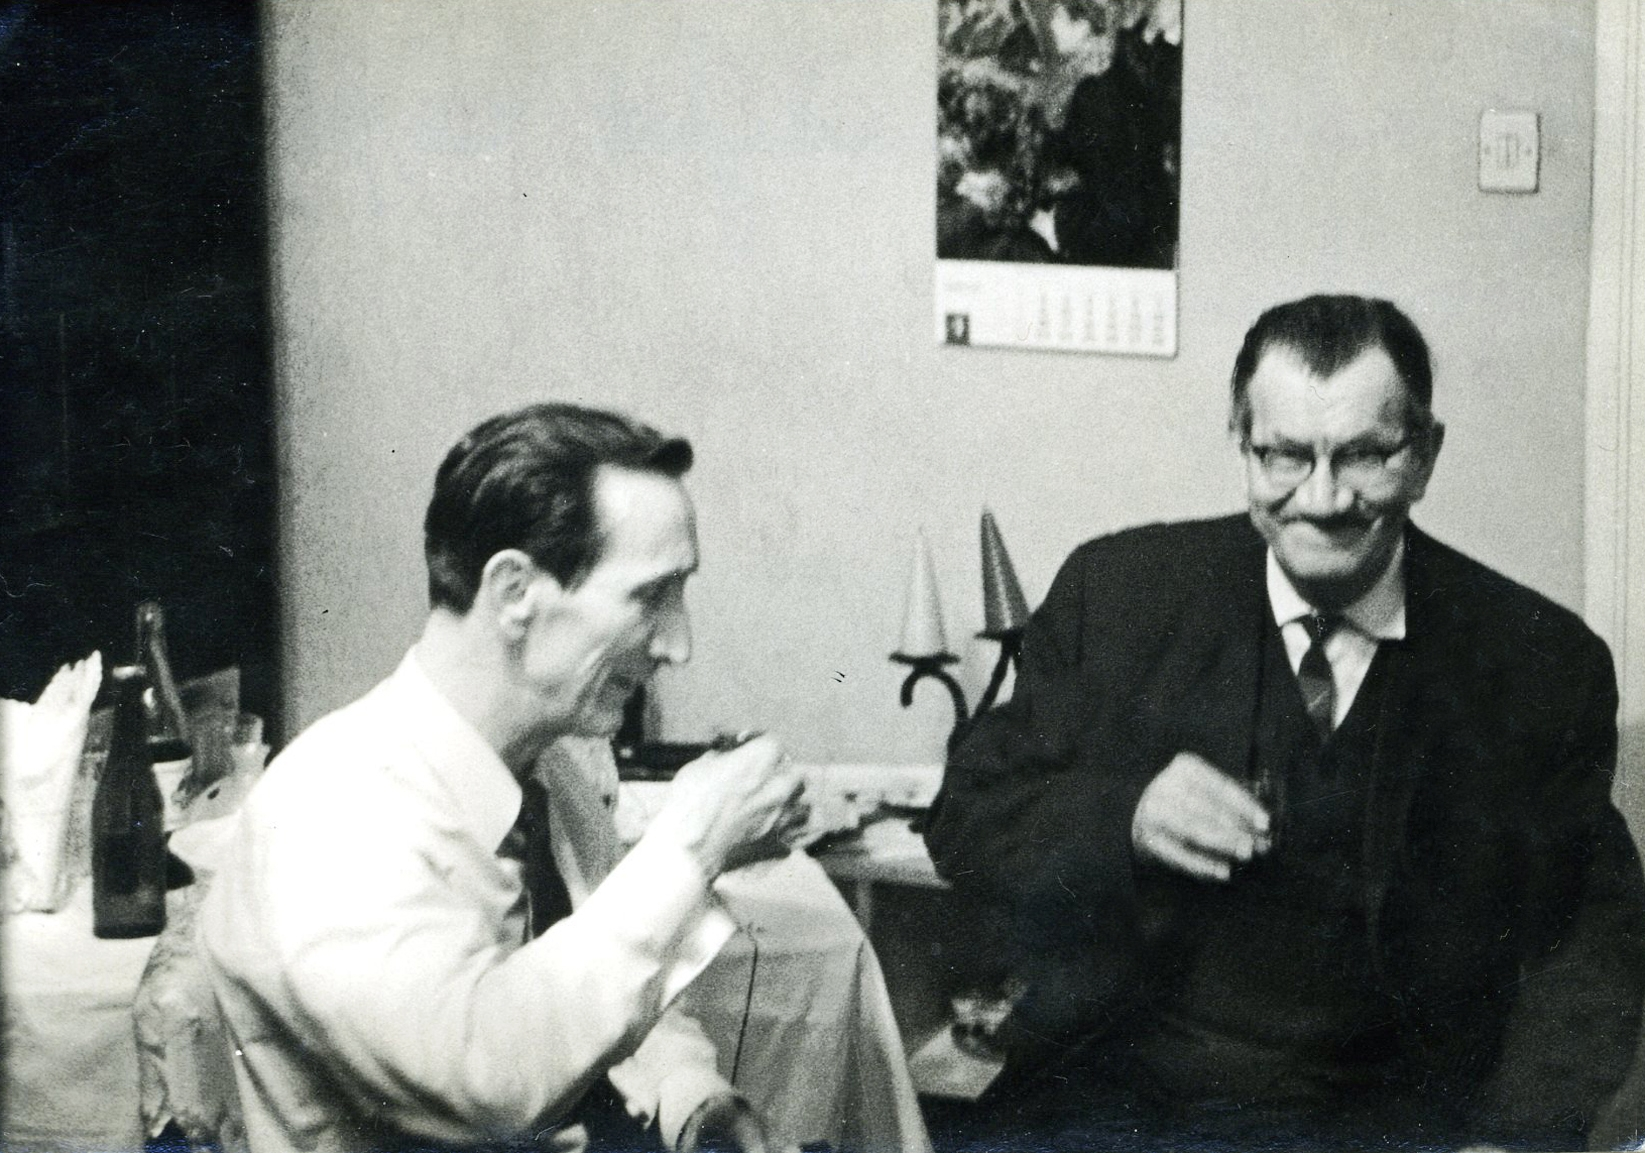
\includegraphics[width=0.6\textwidth]{photo/benedykt_jozef_swierczynscy.jpg}
\caption{Józef i Benedykt Świerczyńscy}
\end{center}
\end{figure}

Gdy wreszcie wrócił w marcowy późny wieczór stryj Józef zadał mu sakramentalne pytanie o przyczynę jego nieobecności na tak ważnej uroczystości. W odpowiedzi na jego mętne tłumaczenia oburzony stryj Józef trzepnął naszego Tatę w twarz w naszej obecności. Nastała głęboka konsternacja, po której nasz Tato postawił na stół butelkę, która pomogła im się na powrót pojednać, na tyle, że stryj Józef był na ,,Abrahamie'' swego najmłodszego brata.

\begin{figure}[!h]
\begin{center}
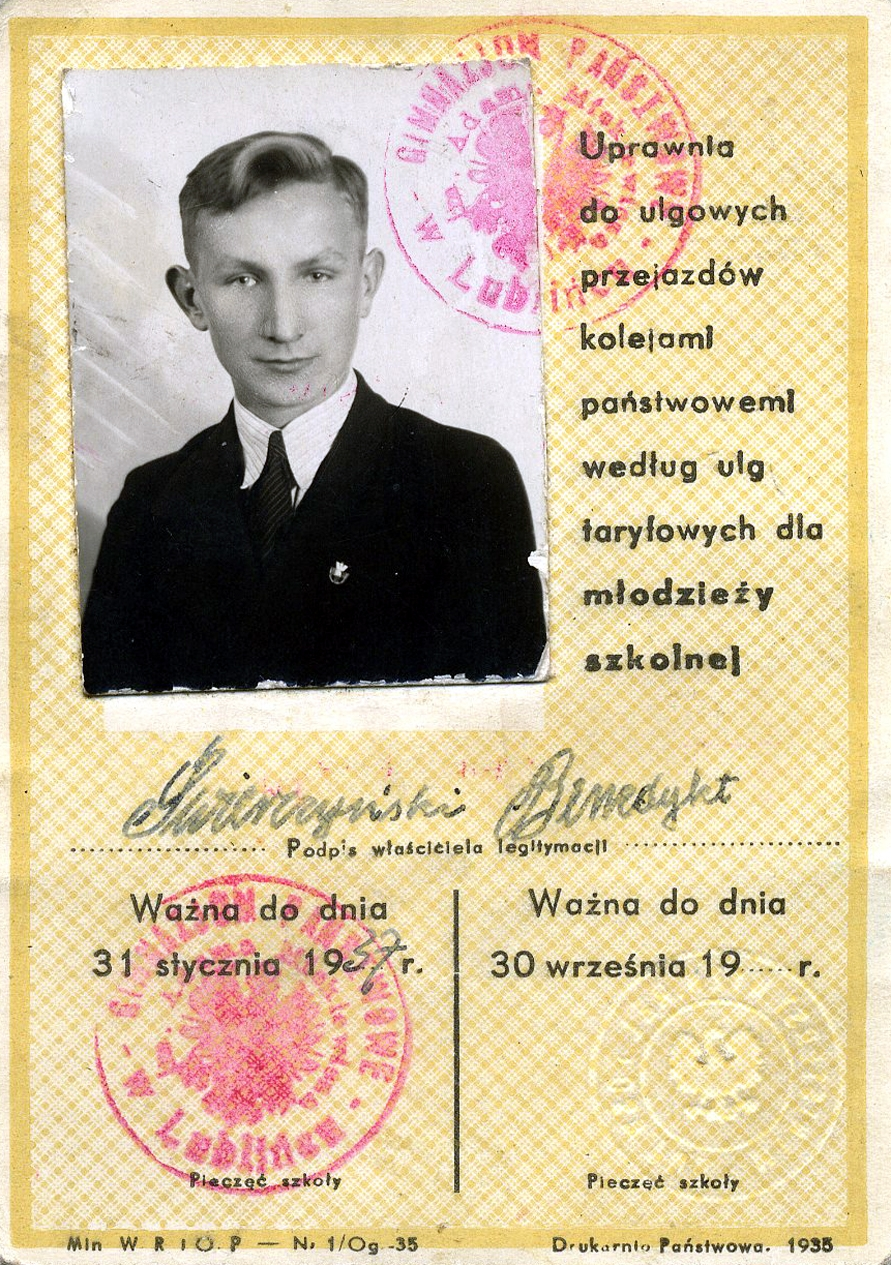
\includegraphics[width=0.6\textwidth]{photo/benedykt_swierczynski_legitymacja.jpg}
\caption{Legitymacja gimnazjalisty - Benedykta Świerczyńskiego.}
\end{center}
\end{figure}

Nasz Tato ukończył gimnazjum i kontynuował naukę w szkole średniej, ale na maturze powinęła mu się noga na języku niemieckim. Musiał zdawać poprawkę, gdy tymczasem wybuchła II wojna światowa. W czasie tych ostatnich w wolnej Polsce wakacji podjął pracę w Wojskowym Instytucie Geograficznym -- na placówce terenowej w Piotrowicach, o której władze Instytutu, jak się później okazało, nie wiedziały. Był to prawdopodobnie bezczelny kamuflaż hitlerowski, mający na celu dokładne określenie współrzędnych obiektów, którymi pewnie była zainteresowana artyleria niemiecka na czas zbliżającej się wojny. Na koniec sierpnia wypłacono mu za tę pracę 85 zł i 31 sierpnia wrócił na Wieski. 1 września była już wojna! Po południu dziewiętnastoletni Benedykt ruszył do Lublińca, by zasięgnąć języka, lecz zobaczył triumfujących Niemców i renegatów spośród polskojęzycznych Ślązaków oraz w wielu oknach powiewające czerwone flagi ze swastyką w centrum (przecież Hitlerowcy byli narodowymi socjalistami, stąd ta czerwona flaga, co się obecnie ukrywa, wpierając wykształciuchom, niestety skutecznie, że Hitler to prawica, ponieważ był faszystą!).

Nasz Tato wspomina, z jakim napięciem słuchało się radia, które niestety informowało o błyskawicznym posuwaniu się Niemców w głąb terytorium naszej ojczyzny. Jednak 3 września radio podało elektryzującą wiadomość o wypowiedzeniu Niemcom wojny przez Francję i Wielką Brytanię, po której niestety nie nastąpiły działania militarne. Na zachodniej granicy Niemiec błogi spokój, gdy wierny sojusznik Francji i Anglii ginął w nierównej walce, zwłaszcza po napaści drugiego socjalisty – Stalina - na Polskę 17 września. Wśród serdecznych przyjaciół psy (tj. socjalistyczne Niemcy i socjalistyczny Sojuz Sowietów) zająca zjadły. \textit{Kochany Zachód stał i tyle – pisze w swym pamiętniku nasz Tato – a kraj, a Polska dogorywała, aby skwitować 17 września dezercją rządu do Rumunii przy jednoczesnym wkroczeniu na ziemie wschodnie Bolszewików. Państwo Polskie faktycznie przestało istnieć. Jeden gorzki żal do wszystkich, łącznie z Panem Bogiem, że przez cały wrzesień dał piękną, ciepłą pogodę i lotnictwo niemieckie bezkarnie dokazywało na polskim niebie, niszcząc, paląc, zabijając wszystko, co żywe, a ,,polskie drogi'' okazały się łatwe dla wszystkich niemieckich pojazdów wojskowych}. 

Mój drogi Tato, pewnie tam w niebie już wiesz teraz jak bardzo się myliłeś. Gdyby Bóg dał zimny i dżdżysty wrzesień, jak to zwykle bywa, daleko więcej Polaków poumierałoby z chorób, zimna, wycieńczenia niż od kul i bomb hitlerowskiej i sowieckiej machiny wojennej. A tak spokojnie wrócił z owej ucieczki Twój brat Józef z rodziną (z dziewięcioletnią Elżunią i czteroletnim Wirgusiem) i twój przyszły teść -- Tomasz Wilczek aż z samego Brześcia, mimo swoich pięćdziesięciu lat.

Co zaś się tyczy rzekomej dezercji rządu polskiego, to historia przyznała rację prezydentowi Mościckiemu, odmówiła jej jedynie, i słusznie, marszałkowi Rydzowi Śmigłemu, jako dowódcy sił zbrojnych Rzeczpospolitej walczącej! I nigdy żaden uczciwy historyk nie usprawiedliwi zbrodniczej napaści Sowietów na Polskę, wypełniających w ten sposób tajne postanowienia paktu Ribbentrop -- Mołotow z 20 sierpnia i depczących jednocześnie postanowienia paktu o pokoju z Rzeczpospolitą Polską. Wszystko po to mój Tato, ,,aby okazały się zamysły serc wielu''! Czyż przed II wojną światową nie myślano o Niemcach jako o najbardziej cywilizowanym narodzie? a co się okazało? Teraz zaś ci Niemcy, którzy powinni pokutować i przepraszać całą niemal Europę za straszliwe zbrodnie, których się dopuścili, zwłaszcza na narodzie żydowskim, polskim oraz narodach wschodniej i południowej słowiańszczyzny, ci Niemcy zamiast tego wmawiają światu, że hitlerowskie obozy koncentracyjne były obozami polskimi i domagają się od nas bezczelnie odszkodowania za wysiedlenie ich ziomków z Ziem Zachodnich i Północnych! A przecież z tych ziem wysiedlił ich strach przed Sowietami, sami bowiem zwiewali ile sił w nogach przed miażdżącą pięścią sprawiedliwego słowiańskiego gniewu!!! Bóg dał nawet papieża z ich narodu (wprawdzie spośród Bawarczyków – najbardziej duchowo zlatynizowanej dzielnicy Niemiec), lecz nie zdziwię się wcale, gdy pewnego dnia media podadzą, że w Niemczech albo z inspiracji Niemców lub rękami Niemców dokonano skutecznego zamachu na życie Benedykta XVI! \textbf{Wszystko po to, aby okazały się zamysły serc wielu!}

Gdy Berlin ogłosił dekret o włączeniu do Rzeszy Górnego Śląska i Pomorza Gdańskiego nasz Tato wybrał się rowerem do Piotrowic, do stryja Józefa z walichą pełną tego, co wieś daje zwykle miastu. Trafił akurat na moment, kiedy wrócili oni z ucieczki przed frontem, ale front ich prześcignął nim zdołali dotrzeć do Krakowa. Opowiadał stryj Józef \textit{jak to drogi zatarasowały chłopskie furmanki nieraz z całym dobytkiem i jak co chwila samoloty niemieckie urządzały sobie polowania na tę masę ludzi zostawiając po sobie śmierć i nieszczęście}. Wspominał też nasz Tato ze wstrętem o tych wszystkich polskojęzycznych Ślązakach, którzy na fali zwycięstw Hitlera starali się ze wszystkich sił zostać Niemcami, zniżając się do najgorszej nawet podłości. I wspomina nasz Tato z satysfakcją, że nikt z tych zaprzańców nie zrobił kariery, a większość z nich zginęła w niesławie za Führera\ldots

\begin{figure}[!h]
\begin{center}
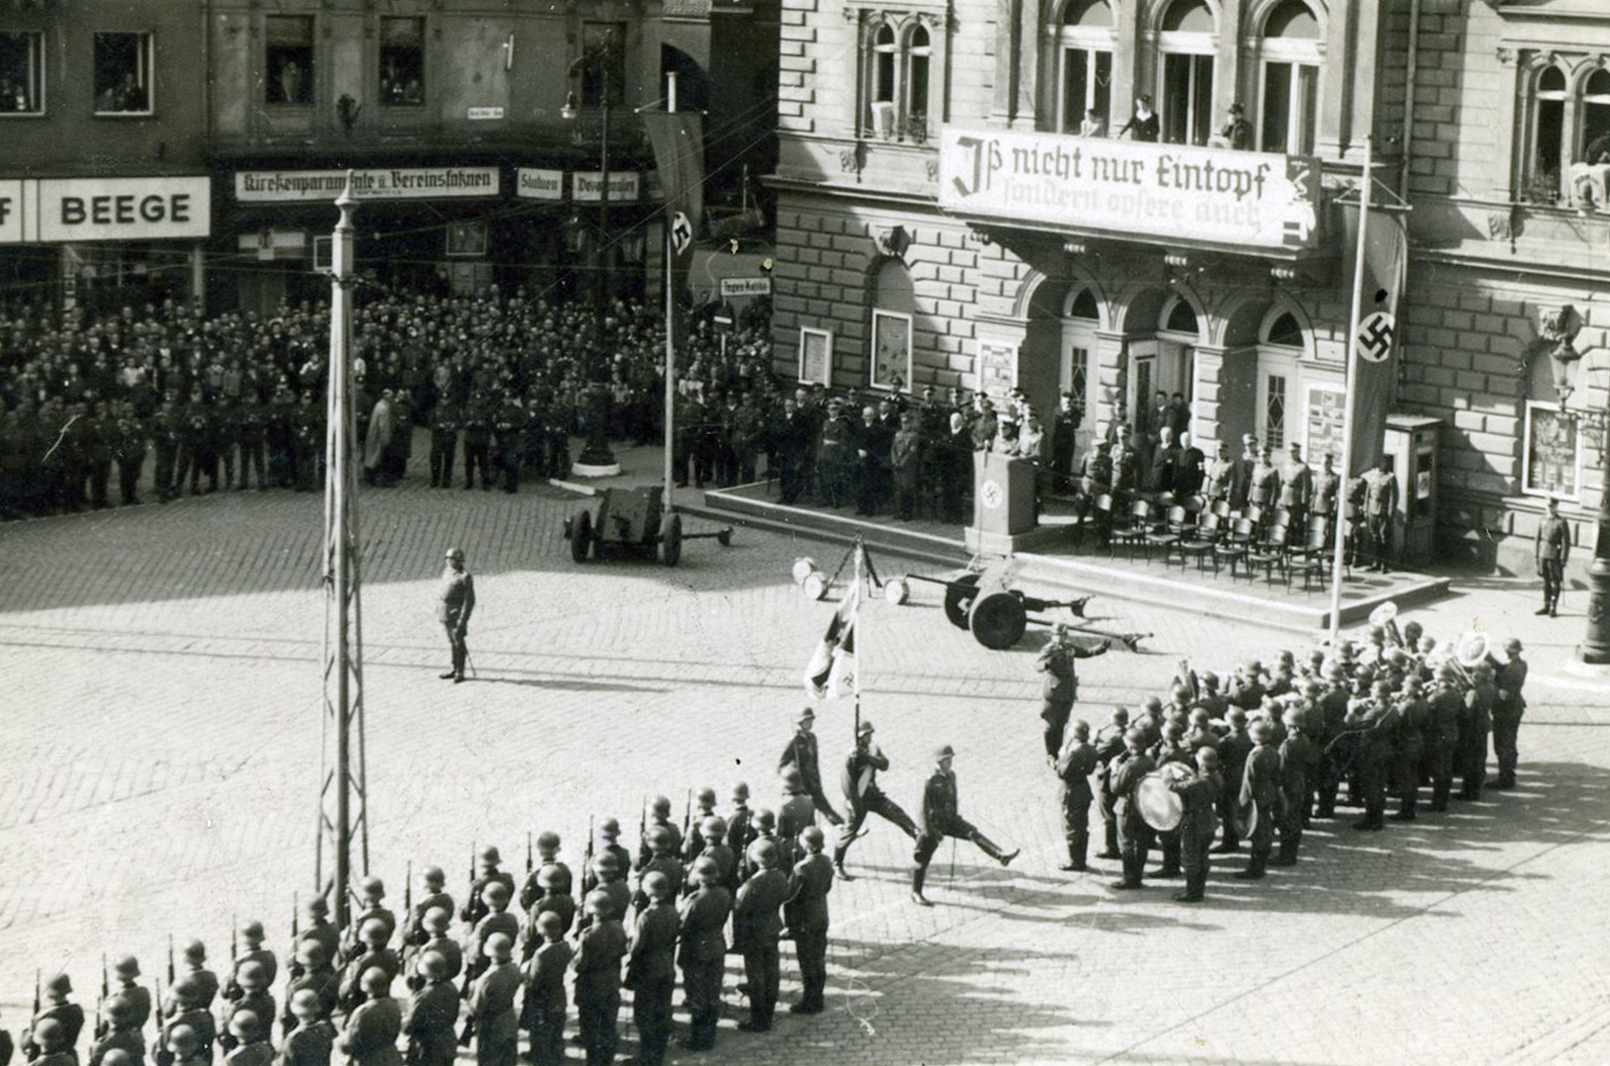
\includegraphics[width=0.7\textwidth]{photo/lubliniec_okupowany.jpg}
\caption{Okupowany Lubliniec}
\end{center}
\end{figure}

Po sromotnej klęsce Francji zakończonej kolaboracją marszałka Petaina, premiera rządu w Vichy uległego Hitlerowi -- nasz Tato, nie widząc nadziei na rychły upadek Hitlera, uchwycił się jak tonący brzytwy proroctwa o ,,Polsce od morza do morza, którą bronić będzie sława i łaska Boża'' oraz o tym, że ,,gdy czarny orzeł wzrok swój na wschód obróci, ze złamanym skrzydłem powróci'' i poszedł z nim do księdza Jana Banasia, proboszcza w Lubecku, lecz ten zgasił jego nadzieje pytaniem o liczbę czołgów i samolotów, które mogą wyprodukować Niemcy\ldots

\begin{figure}[!h]
\begin{center}
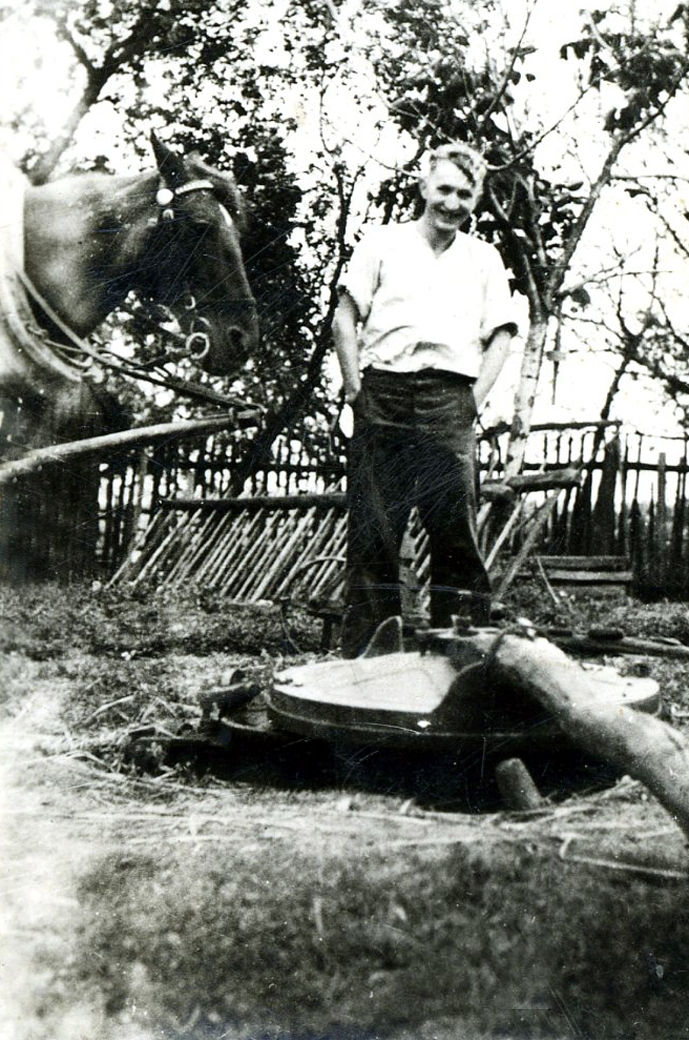
\includegraphics[width=0.4\textwidth]{photo/benedykt_swierczynski_przy_kieracie.jpg}
\caption{Benedykt Świerczyński przy kieracie na ojcowej gospodarce}
\end{center}
\end{figure}

\begin{figure}[!h]
\begin{center}
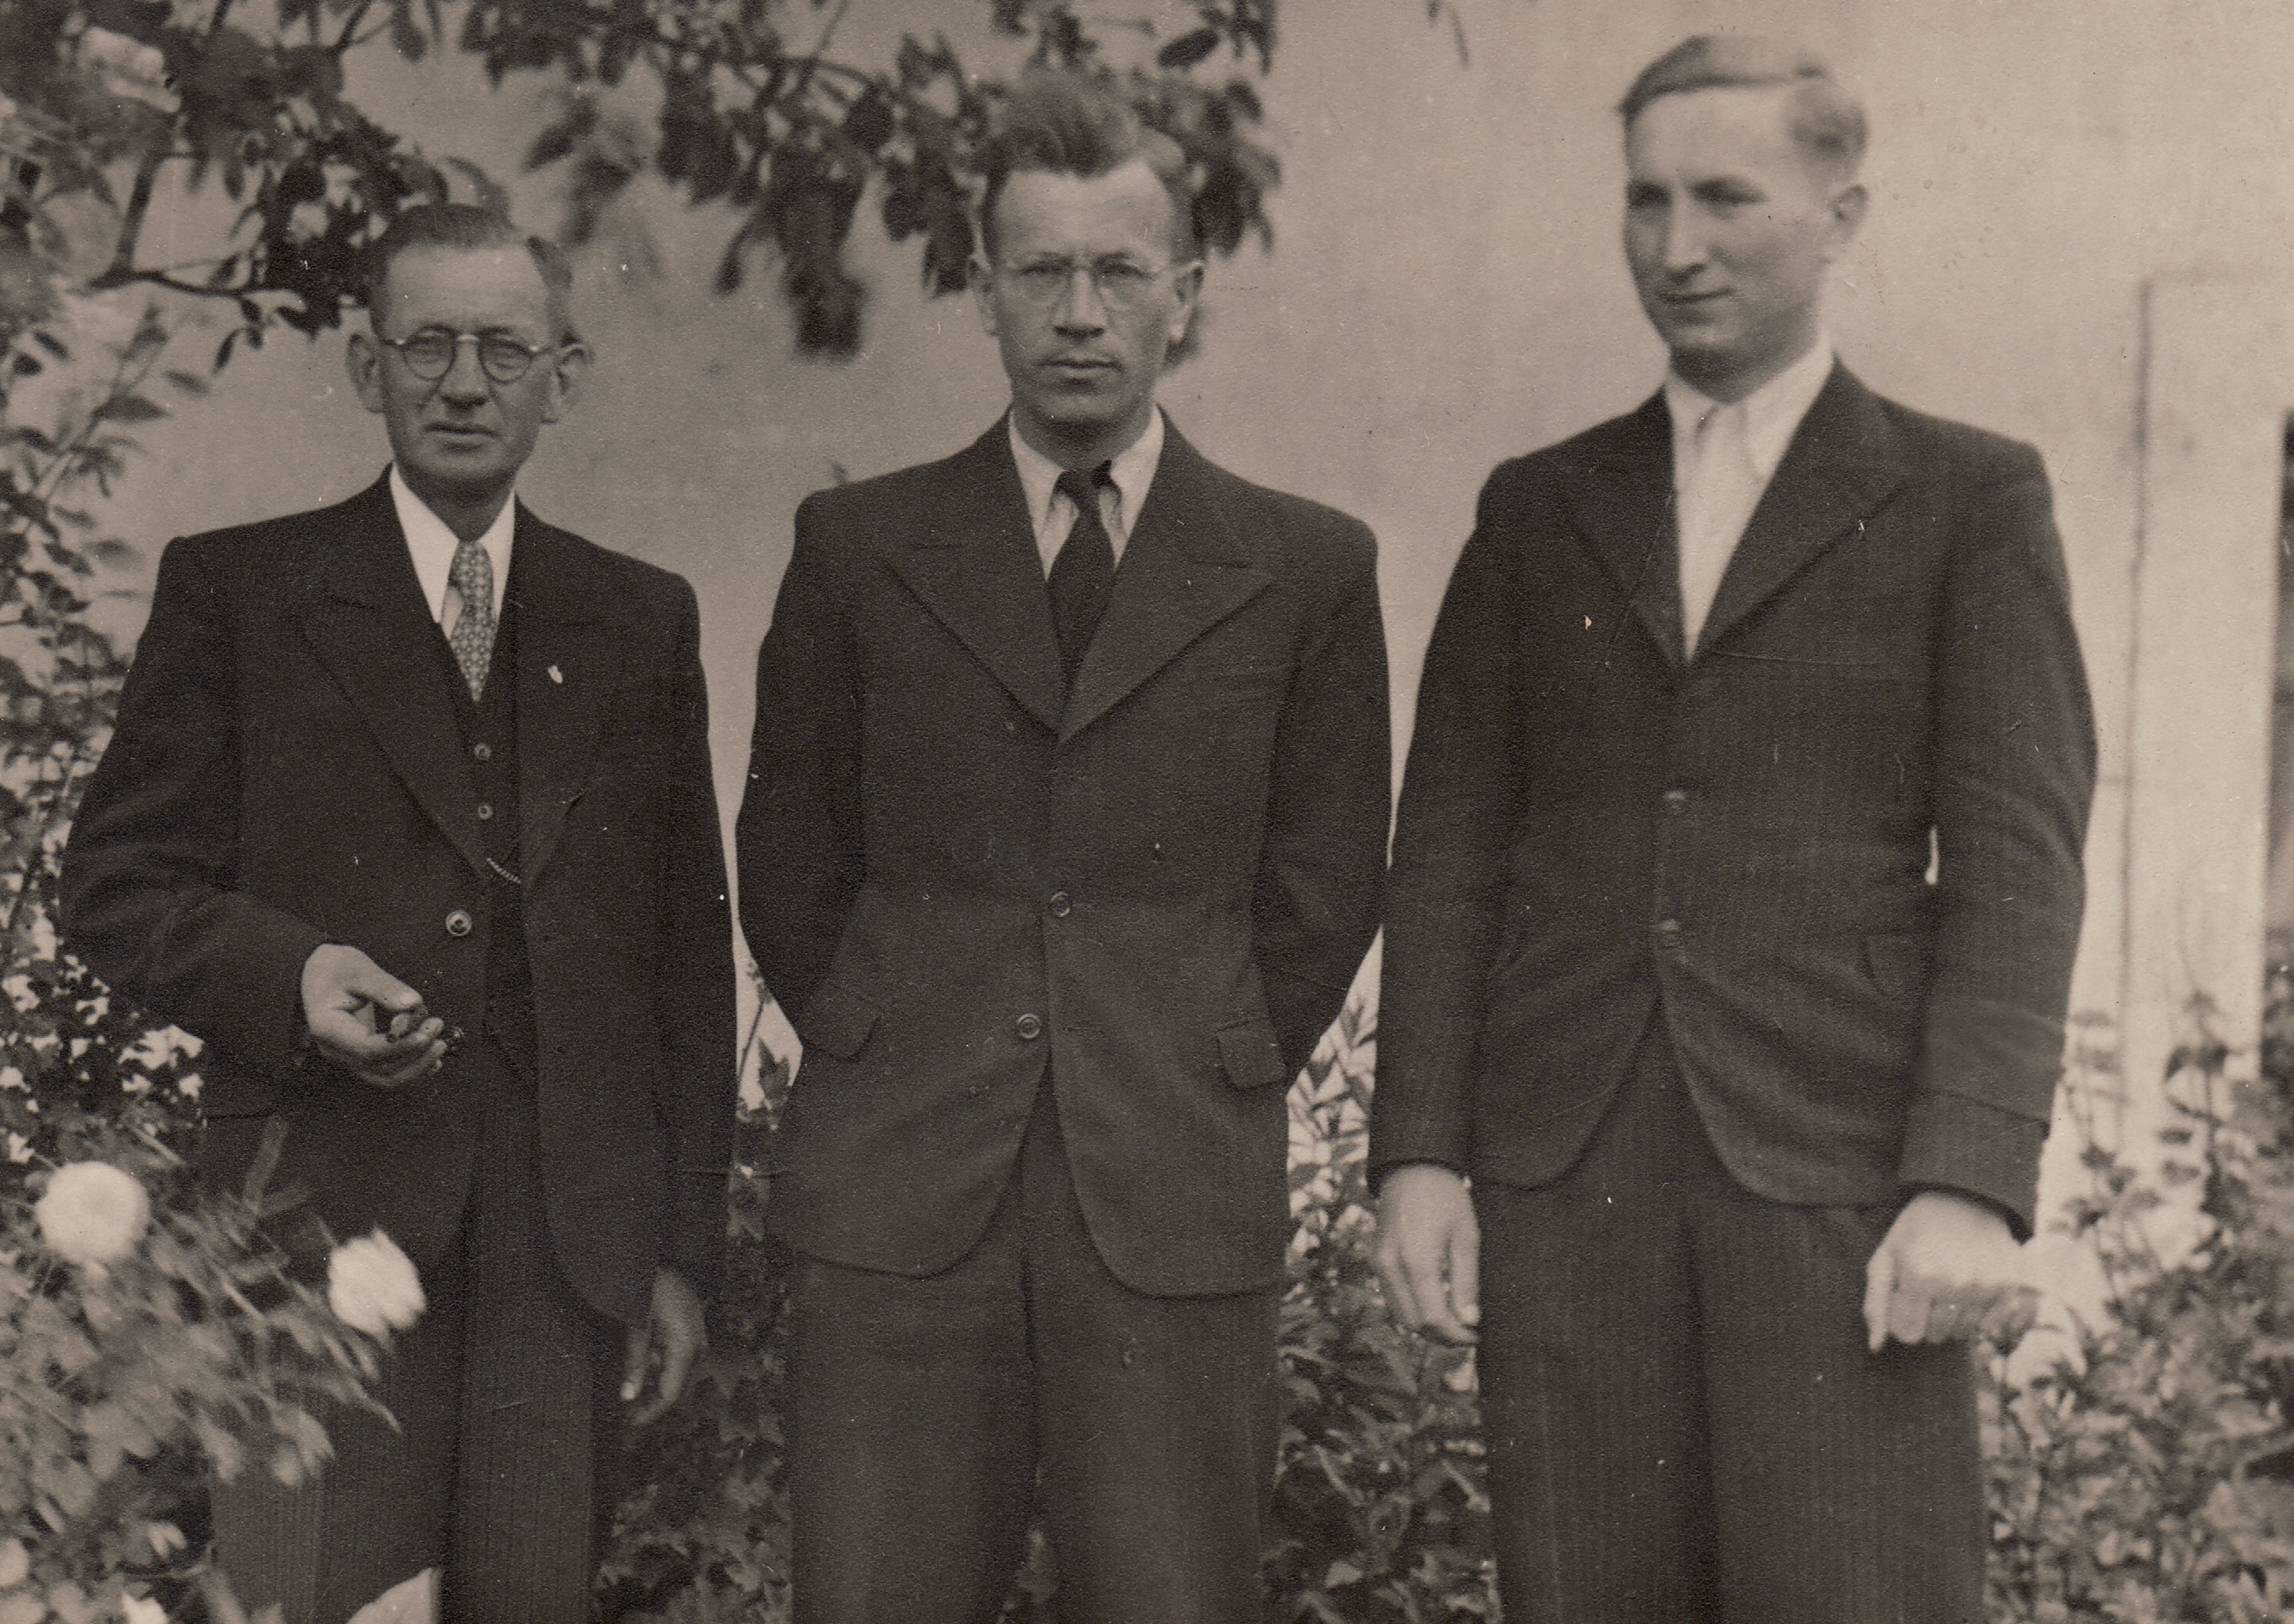
\includegraphics[width=0.7\textwidth]{photo/benedykt_swierczynski_z_wujkiem_kusztantem.jpg}
\caption[X. Grabiński, Józef Świerczyński i Benedykt Świerczyński]{Na zdj. od lewej: X. Grabiński, Józef Świerczyński i Benedykt Świerczyński}
\end{center}
\end{figure}

Nasz Tato nie miał tej wiary, co nasz dziadek Tomasz Wilczek, który do końca życia ufał, że Polska będzie od morza do morza. Toteż gdy wkrótce po haniebnym upadku Francji, odbyła się narada rodzinna z udziałem dziadka Edwarda, braci Józefa i Wiktora, szwagra Antoniego Lehmana, kuzyna Jerzego Wąsa i wujka Kusztanta, zakończona stwierdzeniem tego ostatniego, że ,,jedyna nadzieja w bolszewiku'' - załamał się i bez żadnej już nadziei oczekiwał z lękiem na pismo o powołaniu do Wehrmachtu. Niechybnie też ono nadeszło, zobowiązując rekruta Benedykta Świerczyńskiego, by stawił się dnia 10 października 1940 r. przed budynkiem lublinieckiego dworca. Gdy wieźli ich do Opawy, ostatni raz po polsku wyśpiewali wszystkie znane im śląskie pieśniczki. Tam czekał ich niesłychany rygor. Dane mu było służyć w jednej drużynie ze szkolnym kolegą -- Emilem Masoniem. W grudniu 1941 r. zostali przewiezieni przez Katowice, Kraków, Tarnów do Szczucina, a stąd pieszo przez Wisłę na wąskotorówkę, którą dojechali do koszar w Staszowie, na Kielecczyźnie\ldots

Tutaj przypadło polskim Ślązakom spędzić Boże Narodzenie. W kościele śpiewali z pamięci wszystkie polskie kolędy, co zwróciło na nich uwagę miejscowej ludności. Na odwagę zdobyła się pewna młoda kobieta, która zapytała naszego Tatę dlaczego on Polak ( bo śpiewa poprawnie polskie kolędy) przywdział mundur niemiecki. Jego tłumaczenie, że w wyniku działań wojennych stał się obywatelem III Rzeszy i jako taki został zmuszony do służby wojskowej w Wehrmachcie zostało przyjęte ze zrozumieniem. Wraz z kolegą Wiktorem Kokotem został zaproszony do jej domu przy ul. Stodolnej. Po pierwszym spotkaniu, które trwało niecałe dwie godziny dobrali do swego towarzystwa jeszcze Franka Szymańskiego, z którym na wiele miesięcy i lat połączyły naszego Tatę więzy serdecznej przyjaźni. Powoził on kuchnią polową i miał dobry dostęp do magazynów żywnościowych, dzięki czemu mógł dla gościnnych Polek ,,wycyganić'' cukier. W czasie tych niedzielnych spotkań wzajemnie się pocieszali. \textbf{Stamtąd otrzymał nasz Tato 14 dni urlopu}, więc ,,w te pędy'' \textbf{do Katowic -- Ligoty}, do stryja Józefa i dalej do kochanych rodziców, na \textbf{Wieski} i by posłuchać radia stryja Wiktora. Lecz wtedy Niemcy były niestety u szczytu potęgi!

Na początku marca całe wojsko przemaszerowało 60 km do \textbf{Ostrowca Świętokrzyskiego}, a na początku kwietnia w Wielki Tydzień pomaszerowali dalej na wschód do \textbf{Lublina}. Tam w Wielką Sobotę, Niedzielę i Poniedziałek Wielkanocny 1941 r. można było wyjść na miasto i do kościoła. Mieli tam stacjonować już na stałe, lecz pod koniec maja wyszli i przez \textbf{Chełm, Hrubieszów dotarli nad sam Bug}. Od Ostrowca Świętokrzyskiego mieli już ćwiczenia z użyciem ostrej amunicji, lecz nikomu do głowy nie przychodziło, że Hitler zaatakuje Związek Sowiecki\ldots Jednak 21 czerwca wieczorem odczytano całemu wojsku rozkaz Führera o wojnie z ZSRR, która miała się rozpocząć o 3 rano, a jej pierwszym celem było \textbf{sforsowanie Bugu}, zajęcie \textbf{Uściługu} i rozwinięcie natarcia na \textbf{Włodzimierz Wołyński}. I wszystko po to, by na koniec, gdy trafi  zabłąkana kula, rodzina otrzymała wiadomość, ,,żeś poległ za Führera, Volk und Vaterland''\ldots (wspomina z bólem nasz Tato).

Po sforsowaniu Bugu przeżył nasz ,,Wojak'' wielki chrzest bojowy pod strasznym nocnym ostrzałem artyleryjskim. Miał wielkie szczęście, że dowódcą jego plutonu był nad wyraz spokojny Niemiec z Kluczborka -- Rösner. W południe nadjechała najbardziej oczekiwana przez jego dowódcę ,,Gulaschkanona'', którą powozili Herman Górecka i Franek Szymański. Ponieważ wielu wtedy zginęło była również repeta.

\begin{figure}[!h]
\begin{center}
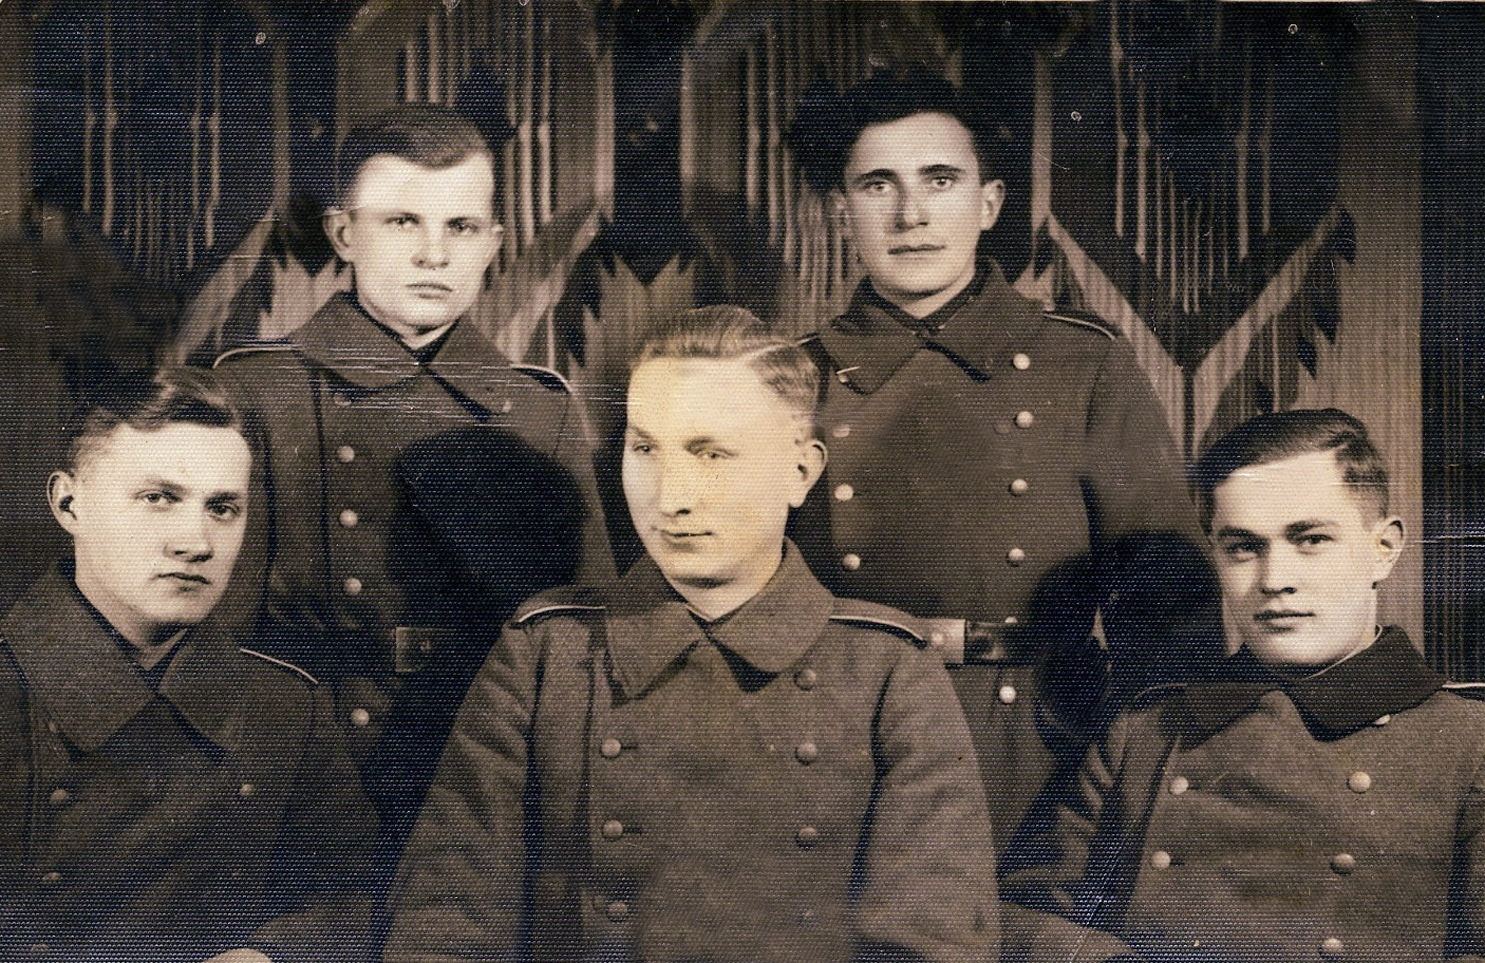
\includegraphics[width=0.7\textwidth]{photo/benedykt_swierczynski_wojna.jpg}
\caption{Benedykt Świerczyński wśród kolegów frontowych}
\end{center}
\end{figure}

,,Włodzimierz Wołyński zdobyli pancerni i jakaś zmotoryzowana piechota.'' Dowiedzieli się, że mieściła się tam sowiecka szkoła artyleryjska, która ich w nocy tak okropnie wytarmosiła. Dalej był \textbf{Łuck} trochę postrzelany, \textbf{zerwane mosty na Styrze} (a więc były tam niemałe boje) i jeszcze \textbf{Korzec} z jakimś zamczyskiem z białego kamienia i wnet stara granica polsko – sowiecka. Zatrzymali się dopiero na 2~-~3 tygodnie pod Korostyniem, gdyż Sowieci przestali się cofać. Nasz Tato czując wielki głód najadł się surowych buraków, które wywołały u niego biegunkę, jak przy czerwonce, więc go dowódca wycofał na tyły i \textbf{do szpitala w Nowogrodzie Wołyńskim}, na oddział zakaźny. Tymczasem artyleria sowiecka zamieniła las pod Korostyniem dla ich dywizji w ,,Totenwald''. Spośród 90 żołnierzy zostało tylko 36, zginęło aż 32! Zginął tam też dowódca jego plutonu wraz z amunicyjnym, który na czas domniemanej czerwonki zastąpił naszego Tatę. Polubił za to mój Tato czerwone buraczki, o Panu Bogu nie wspomniał, a przecież to On wywołał w nim apetyt na surowe buraki, by dzięki nim nie znalazł się w miejscu szczególnego zagrożenia życia! (Ileż modlitw za niego zanosiły do Boga jego matka Eufemia i siostry)

Ich dywizja strasznie poszarpana w \textbf{,,Totenwaldzie'' pod Korostyniem} szła od tej pory w odwodzie, za frontem, czekając na uzupełnienia, które ,,niestety'' jeszcze \textbf{przed sforsowaniem Dniepru} nadeszły. ,,Znowu ich kompania miała stu chłopa'' i większość nowych ludzi, których straszono okropnymi obrazami wojny. Wnet, pod koniec lata 1941 r. sforsowano \textbf{Dniepr i Desnę}. Na wschód od Desny ich pułk miał zamknąć od północy okrążenie kilku armii sowieckich (ok. 600 – 700 tys. żołnierzy). Z równiny płaskiej jak stół wznosiło się niewielkie wzgórze porośnięte lasem z zabudowaniami, który miał obsadzić pluton naszego Taty. Zdesperowani żołnierze sowieccy, chcąc się przebić przez okrążenie urządzili ich armii straszną rzeź, w której zginęło mnóstwo Niemców i Rosjan straszliwie pokiereszowanych. Natomiast na owym zalesionym wzgórzu mnóstwo żołnierzy sowieckich poddało się ich plutonowi.

Tak po raz kolejny Opatrzność Boża, poprzez rozkaz dowództwa postawiła Go w miejscu najmniej narażonym na ostrzał wroga. Do końca wojny nasz Wojak nie widział tylu zabitych, rozjechanych przez czołgi, tyle rozbitego sprzętu wojennego. Wyrwało się wtedy z tego okrążenia około 170 tys. żołnierzy sowieckich, lecz za jaką cenę?! To była masakra! Przed południem przyjechał z kuchnią polową Franek Szymański i przywiózł list od stryja Wiktora nakłaniający naszego Wojaka do chronienia przede wszystkim własnej głowy, bo nie ma dla kogo ginąć, gdyż reżim hitlerowski jest gorszy nawet od bolszewickiego. Po przeczytaniu tego listu Frankowi Szymańskiemu, zaraz go spalili. Lecz od tej pory wiedzieli, co im czynić przystoi. Tym bardziej, że utwierdził ich w tym przekonaniu jakiś podporucznik, który wygłosił dla żołnierzy ich pułku wykład na temat wschodniego teatru wojny. Mówił on, że czeka Niemcy długotrwała i wyczerpująca wojna z Sowietami.

Tymczasem armia niemiecka parła dalej na wschód poprzez nasze dawne wschodnie rubieże Rzeczypospolitej Szlacheckiej, tj. \textbf{przez Perejasław, Łubnie i Połtawę dotarli gdzieś na południe od Charkowa}, lecz nastały deszcze i czarnoziem ukraiński stał się błotnistą mazią uniemożliwiającą poruszanie się ogumionych pojazdów. Na początku listopada, gdy to błoto nieco przymarzło dotarli aż nad Doniec. Siedzieli po chałupach, a nasz Tato uczył się czytać po rosyjsku i pytać, jak im się żyje. Gdzieś w grudniu przeprawili się na \textbf{wschodni brzeg Dońca} i tam dotrwali aż do pierwszych tygodni stycznia 1942 r. Mróz był siarczysty, ale zupełna cisza na ich froncie.

W połowie stycznia, chcąc zdobyć języka, dowódca ich plutonu zastrzelił jednego Ruskiego, a drugiego żywcem zgarnęli. Lecz w dwa dni później Ruscy wzięli o wiele potężniejszy odwet, mianowicie zabrali cały sztab pułku wraz z mapami sztabowymi, szyframi itd. Wkrótce też zaczęło się sowieckie kontrnatarcie. Pułk naszego Taty był najdalej wysunięty na wschód, bo aż za Doniec, więc uciekał najszybciej ,,na z góry upatrzone pozycje\ldots'' a mróz był okropny. Oddział Taty został wysłany na zwiady do pewnego lasu. Lecz w tym popłochu wkrótce w kompanii zapomniano o nich. Gdy wyszli z owego lasu, już po ich pułku nie było śladu. Więc gonili ile sił w ten siarczysty mróz, aż dopadli ,,swoich''. Ruscy ciągle atakowali, ciągle ich pędzili tak, że niemieckie lotnictwo pomyłkowo zbombardowało swoją formację kwatermistrzowską. Tak uciekając dzień i noc prawie bez odpoczynku natknęli się na rozbity samochód niemiecki z konserwami i sucharami. I dalej zmykali\ldots aż pewnego razu trzy czołgi sowieckie T-34 oddzieliły ich kompanię od reszty pułku. Schronili się do głębokiego jaru, którego te czołgi już nie mogły sforsować. Wreszcie kolejną nocą maszerując, dotarli do stacji \textbf{Łozowaja} -- ważnego węzła kolejowego. Lecz i tu nie zastali swego pułku, więc dalej w nogi w kierunku \textbf{Pawłogradu}. Tak pędząc nareszcie dołączyli do swego pułku\ldots I tutaj jakże radosne spotkanie z kuchnią polową, Frankiem Szymańskim i Hermanem Górecką. 

Niestety po dwóch godzinach znowu wymarsz, kolejny czwarty, czy piąty dzień i noc w marszu! Wreszcie \textbf{dotarli pod Pawłograd}. Tutaj rozhulała się zima na dobre. Mróz wprawdzie zelżał, ale śniegiem tak sypnęło, że żadne środki transportu nie były w stanie przezeń się przedrzeć. Front stanął, ale Sowieci zbombardowali wielki niemiecki skład amunicji. Dopiero z początkiem marca Niemcy ruszyli na wschód ,,odzyskiwać'' zimą utracony teren. Stoczono krwawą bitwę \textbf{o Łozowaję}, lecz nie zdobyto tego miasta. Potem do maja znowu spokój. I w maju, podczas jednego z natarć niemieckich naszego Tatę trzasnął w rękę i w saperkę granat moździerzowy.

Został ranny i trafił do szpitala w \textbf{Dniepropietrowsku}, a stamtąd do szpitala ,,w kraju'', więc długa podróż przez \textbf{Czerkasy, Fastów, Winnicę, Tarnopol, Lwów, Przemyśl, Kraków, Katowice, Opole, Wrocław, Jelenią Górę, Görlitz, Drezno, Erfurt, Eisenach, Fuldę, Frankfurt nad Menem, Koblencję} i ,,przepięknym przełomem Mozeli'' do \textbf{Traben -- Trarbach}, do małego szpitaliku, w którym powracał do zdrowia, dzieląc pokój z ,,porządnym karlusem'' z Byczyny. Tam otrzymał po wygojeniu rany dwutygodniowy urlop zdrowotny, a ponieważ dotarły do naszego Taty niepokojące wieści o stryju Wiktorze, więc w te pędy ruszył z \textbf{Bulay} ,,urlauberem'' w strony rodzinne -- \textbf{do Łagiewnik}, na Wieski. 

W domu same zmartwienia: o Karliku słuch zaginął, Józef w wojsku na dalekim zapleczu, więc trzeba dbać o wielką rodzinę w mieście, mimo że zarekwirowano naszemu dziadkowi -- Edwardowi jego gospodarstwo -- wszystkie sztuki żywca policzone -- spróbuj którą ruszyć. Zaraz też, przy pierwszej sposobności nasz Tato odwiedził w szpitalu psychiatrycznym stryja Wiktora. Ledwie go poznał! Żywy trup! Mówił z trudem, a tak chcieli sobie pogadać\ldots Odwiedził też \textbf{w Lublińcu} swoją panią profesor języka niemieckiego -- pannę Peterkównę, która okazała się wielką patriotką! Zajrzał również -- na prośbę Franka Szymańskiego -- do jego sympatii, która młodego wojaka wyraźnie kokietowała, lecz nasz Tato był bardziej wierny swemu przyjacielowi niż ona swemu kochankowi, bo gdy ów Franek wrócił z wojny, ale bez nogi, to ona mu powiedziała, że takiego chłopa, to ona nie chce\ldots

Skończył się urlop i nasz Rekonwalescent musiał wracać do Metzu, gdzie formował się pułk zapasowy, do którego został przydzielony. Tam dopadła go tragiczna wiadomość o śmierci brata Wiktora! Hitlerowscy ,,lekarze'', w tym dyrektor Szpitala Psychiatrycznego w Lublińcu -- dr Buchalik -- zabili Go zastrzykiem fenolu w serce. Zmarł 24 czerwca 1942 r.\ldots Nasz Tato nie mógł dostać urlopu na okoliczność śmierci brata, tym bardziej, że telegram szedł do Metzu aż dwa dni. Pogrzeb odbył się 27 czerwca. Urlop, który jednak otrzymał, ale już po pogrzebie brata, przebiegł w ponurym nastroju.\ldots W Katowicach -- Ligocie dowiedział się od szwagierki stryja Józefa -- Geni o Oświęcimiu! ,,Przerażające i nie do uwierzenia, a jednak najprawdziwsze były to wieści!'' Podczas tego drugiego urlopu nasi przyszli rodzice wyznali sobie miłość i obiecali, że będą czekać na siebie\ldots Nastały wkrótce pożegnania -- najtrudniejsze z mamą -- naszą babcią Eufemią\ldots

I ponownie trzeba było włożyć na siebie to paskudztwo -- mundur żołnierza Wehrmachtu, potem \textbf{powrót przez Opole, Wrocław ,,urlauberem'' do Metzu, do koszar}. Gdy tam ogłoszono, że poszukuje się ochotników do Afrika – Korps, nasz Tato zgłosił się jako jeden z pierwszych, ale chętnych było mnóstwo, tak bardzo wszyscy bali się ,,Ostfrontu''. Lecz nikogo z Górnoślązaków nie wybrano do tej formacji -- nie mieli zaufania. W zamian za to nasz Tato trafił do ,,Marschbatalionu kierowanego właśnie na Ostfront''. Stacja załadowcza była w miasteczku \textbf{Biez, leżącym na samej linii Maginota}, dzięki czemu mógł nasz Wojak obejrzeć potęgę tych niesamowitych umocnień, co spowodowało, że wyparowały zeń resztki sympatii dla zniewieściałych Francuzów, którzy dysponując takim uzbrojeniem i umocnieniami w kilkanaście dni oddali się Hitlerowi, jak jaka kurtyzana\ldots

Pociąg bez kuchni ponownie ruszył gdzieś na przełomie lipca -- sierpnia na wschód przez \textbf{Koblencję, Moguncję, Frankfurt, Würzburg, Norymbergę, Ratyzbonę, Hof, Chemnitz, Görlitz, Jelenią Górę, Opole, Pawonków, Lubliniec}. Tu na dworcu spotkał wujka Edwarda Grabińskiego zwanego ,,Piekorzem'', który mu naopowiadał wiele pocieszających wieści z różnych frontów, o polskiej i jugosłowiańskiej partyzantce i obdarował naszego Tatę sporym zapasem papierosów\ldots

\textbf{Z Lublińca pociąg przez Herby, Częstochowę, Warszawę, Brześć, Mińsk, Bobrujsk dotarł do Żłobina nad Dnieprem}, czyli na ,,Ostfront''! Stąd ruszył na północ \textbf{do Orszy} (skąd wywodził się Kmicic - bohater ,,Potopu'') i dalej \textbf{na Smoleńsk}, lecz tu wolta na południe przez stacje: \textbf{Poczinok, Briańsk, Orzeł, Kursk, Charków do Izjum}, spod którego ubiegłej zimy zaczął się ich paniczny odwrót. Tu ponowna zmiana kierunku \textbf{na północny wschód – na Woroneż i dalej przez Kupiańsk, Walujki do Ostrogożska}, gdzie była przesiadka na ciężarówki, które zawiozły ich do linii kolejowej \textbf{Woroneż – Rostów}, a stamtąd pociągiem towarowym do stacji docelowej -- \textbf{do Millerowa, w samym środku łuku dońskiego}. Stamtąd pieszo dotarli do \textbf{Boguczara}. 

W tym \textbf{Boguczarze} -- ,,wcale ładnym miasteczku'' trafił nasz Tata do ,,swojego'' pułku i batalionu, a przede wszystkim spotkał tam Franka Szymańskiego i Hermana Góreckę\ldots Stali rzetelnie -- po niemiecku oszańcowani \textbf{nad prawym, zachodnim brzegiem Donu}. Po jednej stronie mieli Włochów (okropnych niechlujów) i Rumunów, a po drugiej stronie Węgrów. Dowódcą jego drużyny był niejaki Wietschorek z Bytomia mówiący po niemiecku, ale też po Śląsku. Nabrał nasz Tato do niego zaufania, zwłaszcza gdy mu powiedział, że ,,tym drukiem urzędowym -- wnioskiem o volkslistę może sobie dupę podetrzeć, natomiast władzom zwierzchnim powie się, że mu je myszy pogryzły\ldots'' Doczekali tam ostrej zimy, która nastała z początkiem listopada 1942 r. Nudę trwania na posterunku rozpraszały im listy od bliskich i paczki z gęsiną z domu oraz suchą kiełbasą od panny Radinki\ldots

\begin{figure}[!h]
\begin{center}
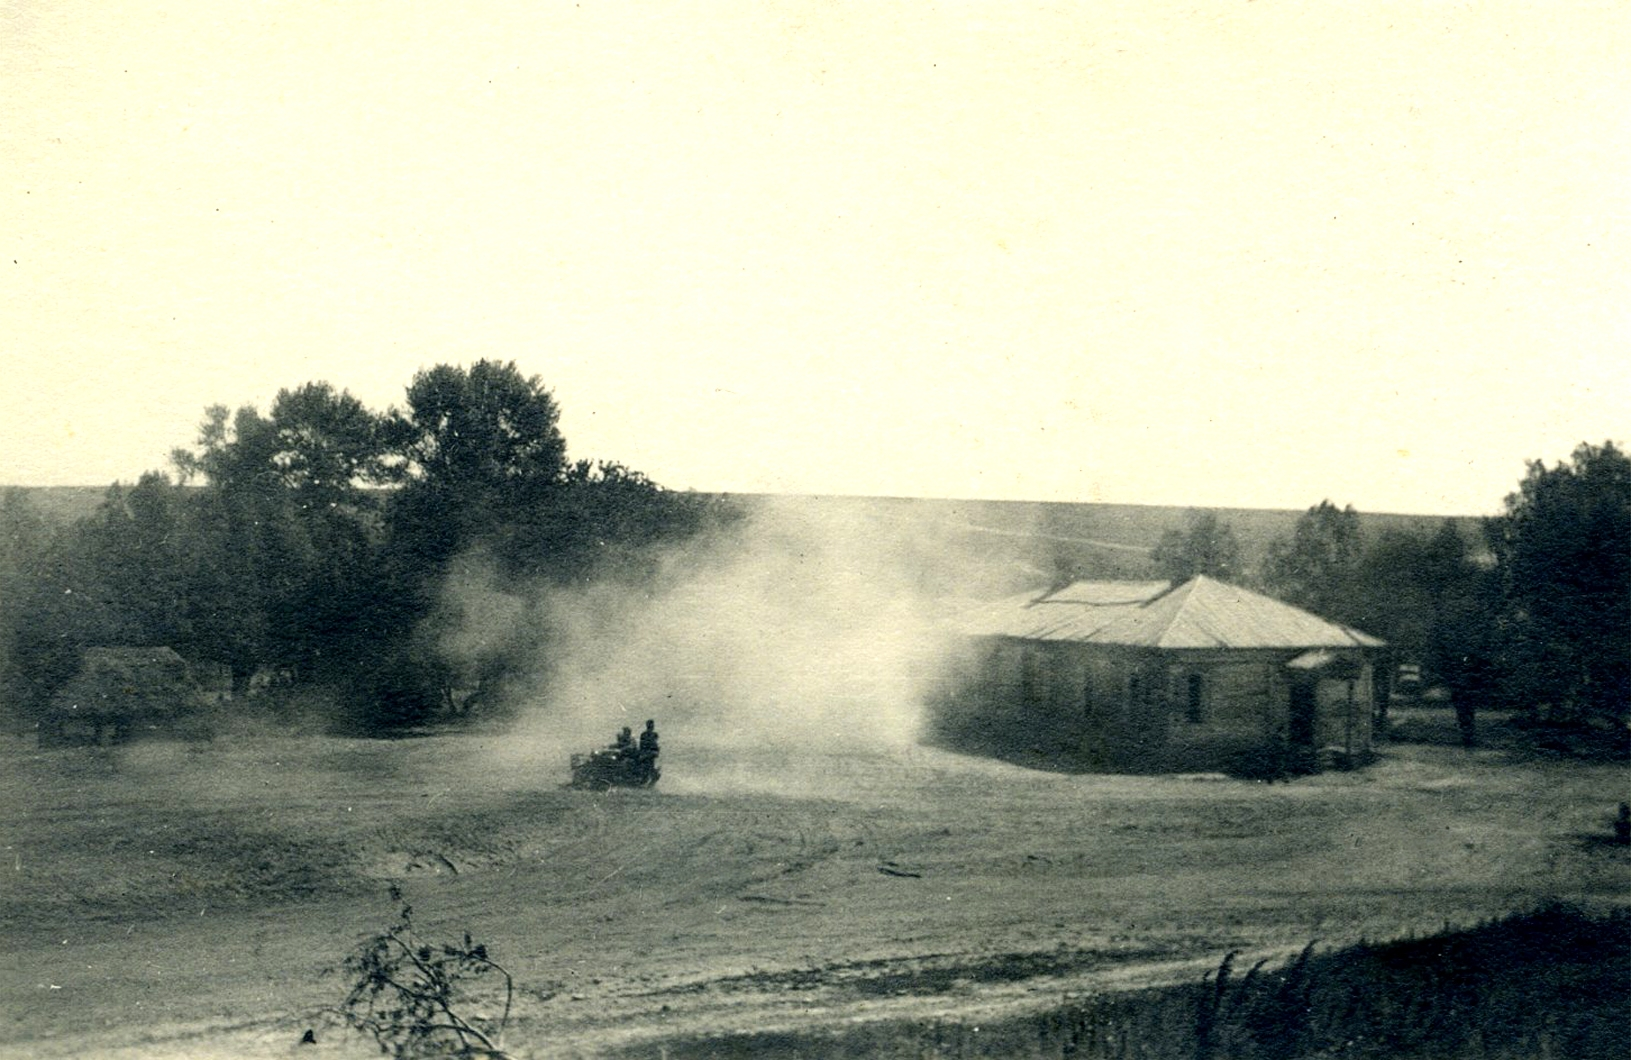
\includegraphics[width=0.7\textwidth]{photo/don.jpg}
\caption{Zdjęcie znad Donu}
\end{center}
\end{figure}

Tymczasem Włosi zrejterowali z lewej -- północnej strony i na wiele kilometrów ich dywizja została odsłonięta. Pewnie dlatego, że Włochów zaatakowali Ruscy. 15 grudnia 1942 r. otrzymał list od stryjenki Ireny, która pisała mu, jak ongiś śp. stryj Wiktor, żeby myślał tylko o tym jak głowę uchronić i żeby pamiętał, co Niemcy z jego bratem zrobili. Pisząc to była przekonana, że jest okrążony w kotle stalingradzkim\ldots 16 grudnia 1942 r. zaczęła się Ruskich kanonada artyleryjska. Pod wieczór ,,był obiad z kuchni i chlebuś'' jak się okazało ostatni i ostatnie z Frankiem Szymańskim spotkanie na wojennym froncie. Na ,,odcinku włoskim'' nadciągała sowiecka piechota, a za nią czołgi i ucieczka ich pułku to w lewo, to w prawo -- jeden straszny krwawy galimatias. Tak przez kilka dni niemal bez jedzenia i spania. Ledwie dopadli jakiegoś domu, gdzie można było się zdrzemnąć, już tam po chwili byli Ruscy. Gdy znowu znalazła się okazja podrzemania w przepełnionym, a więc ciepłym domu, jakiś głos wewnętrzny kazał mu wyjść z niego i podrzemać w dole obok, ogaciwszy się od mroźnego wiatru wiązką trzciny. Upłynęło niewiele czasu, gdy w ten dom trafiło kilka pocisków artyleryjskich, od których spłonął wraz ze śpiącymi tam żołnierzami. Została ich garstka żywych, którzy w pojedynkę, po dwóch uciekali, szukając drogi do ,,swoich''.

Nasz Tato został sam z zamiarem poddania się do niewoli. Odrzucił więc broń, zdjął hełm, włożył furażerkę na głowę i czekał, aż nadejdą Ruscy i wtedy ręce do góry i okrzyk: ,,Nie strielaj, ja odin zdieś, ja choczu w plien''. Prowadzony do sztabu sowieckiego przez jakiegoś ,,dziadka'' natrafił na grupę oficerów, wśród których był Jerzy Borejsza. Ten wypytał po polsku dlaczego on Polak jest w szwabskim mundurze. Wytłumaczył się i dodał jeszcze parę słów o Karliku i Wiktorze oraz także o Andersie, czym sobie zaszkodził. Borejsza poradził mu, by o Andersa więcej nie pytał, dał ,,dziadkowi'' jakąś kartkę i polecił Jeńca zaprowadzić do sztabu. Tam Go przesłuchiwali, ale też nakarmili i trzymali w chlewiku, tj. w areszcie. Dzień później miał już tam sublokatora -- Marcina Krzywonia z Żywca. To była Wigilia 1942 r., a nasz Wojak w chlewie między bydlętami i przy żłobie, w którym siano. Odebrał to jako jakiś dobry znak, symbol dający otuchę, że się przeżyje niewolę i wojnę i powróci szczęśliwie do domu, jak Dzieciątko Jezus z Egiptu do Nazaretu po śmierci Heroda!

W święta Bożego Narodzenia znalazł się w ogromnej kolumnie kilku tysięcy jeńców, głównie krzykliwych Włochów oraz Rumunów. W tej kolumnie trzech tysięcy jeńców znalazł Ślązaków: Borzuckiego z Katowic i z Mysłowic Loskę. Wkrótce dotarli do \textbf{Boguczara}, z którego przed 13 dniami w popłochu uciekali. \textbf{Z Boguczara} przeszli kolumną po moście pontonowym przez Don i szli dalej na wschód aż do \textbf{Kałacza}. W ten sposób  znaleźli się na tym obszarze Rosji, który nie zaznał wojny, Niemców, Włochów, Rumunów. Tu nasz Tato wychodził z Borzuckim żebrać u Ruskich o chleb, o cokolwiek do zjedzenia i...\ldots Rosjanie dawali, mimo że u nich się nie przelewało. Raz ,,babuszka'' w jakiejś wsi dała mu coś do jedzenia, mówiąc: ,,Jedz, ja mam tyle wnuków i wnuczek na wojnie (tu pokazała obydwie dłonie palców) i nie wiem, może oni też są tak głodni jak ty, a ja im pomóc nie mogę, to pomogę choć tobie''-- i popłakała się. Rewanżując się za tak bezinteresowną dobroć ,,cmoknął nasz Wojak babuszkę z dubeltówki, dopił mleko i podziękował, biorąc chleb za pazuchę i szybko z powrotem do kolumny''. \textbf{W Kałaczu} zapakowali ich czwórkę Ślązaków razem z Włochami do bydlęcego wagonu. Tak przez kilkanaście dni jechali na północny wschód przez Penzę \textbf{do Mordwińskiej ASRR, a stąd przez Ruzajewkę do stacji Pot’ma i dalej kilkanaście kilometrów na północ do centralnego obozu jenieckiego w Małocznicy}.

\textbf{Tam spotyka Franka Kępę z Łagiewnik Wielkich}, który w niewoli był już od grudnia 1941 r., a zatem pełnił bardzo przydatną funkcję akwizytora. Wymienili ze sobą informacje. Przydzielono ich do baraków, gdzie było bardzo ciasno, ale za to ciepło i nareszcie bez wszy (gdyż ich ubrania przeszły przez odwszalnię). Francik Kępa oprowadził go po obozie, obdarował go chlebem i przekazał wiele cennych informacji. Wkrótce był przesłuchiwany przez dwie godziny przez jakiegoś Rosjanina, który świetnie znał polski i niemiecki. Często nasz Tato bywał w klubie, gdzie rej wodził \textbf{Leon Fojcik z Rybnika}. Miał on najświeższe wiadomości od Rosjanki – Jadwigi Kreczewskiej, jako że wpadł jej w oko, a ona opiekowała się polską grupą. Ów Fojcik, późniejszy przyjaciel Taty, który bywał u nas w domu - opowiedział mu o kolosalnej klęsce Niemców pod Stalingradem i zobowiązał Go, by opowiadał o niej innym Ślązakom. 

\begin{figure}[!h]
\begin{center}
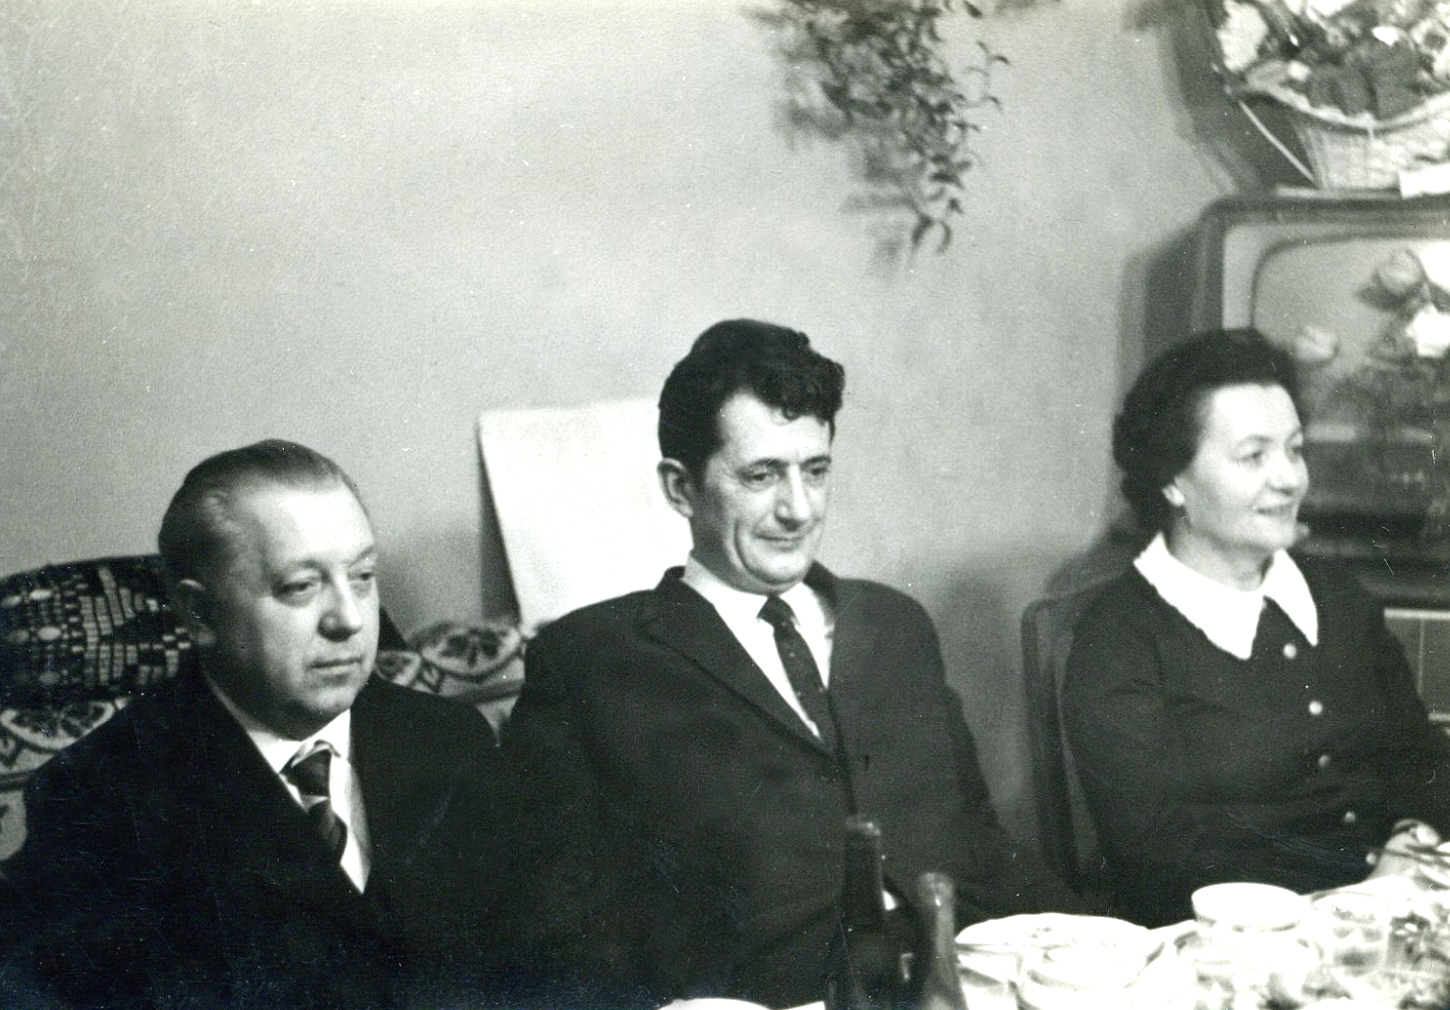
\includegraphics[width=0.7\textwidth]{photo/leon_fojcik.jpg}
\caption[Leon Fojcik z żoną i Rudolfem Juzkiem]{Na zdj. Leon Fojcik z żoną i Rudolfem Juzkiem}
\end{center}
\end{figure}

Gdzieś w połowie marca 1943 r. zostali wszyscy Polacy zgromadzeni w jednym podobozie. Leon Fojcik został tam szefem klubu, Francik Kępa i Jeleń dopadli sanek akwizycyjnych, Broda został kucharzem, Herman chleborezem, \textbf{Rudolf Juzek} starszym pielęgniarzem. Tato był nadal częstym gościem klubu, gdzie było ciepło, a rej wodził tam Leon Fojcik. Zaczął też pracować w ,,fabryce drewnianych łyżek'' za dodatkową strawę. Mistrzami nad mistrze byli tam Finowie. Ustanowiono normę 80 łyżek na szychtę, której nasz Tato nie potrafił wyrobić, więc mu \textbf{Fin Walkonen} dorzucał ze swoich po kilka, by mógł otrzymać ową dodatkową porcję żywności. Kiedy mu jednak pewnego dnia nóż zjechał i wbił się w kolano aż do kości, zrezygnował z pracy w ,,fabryce łyżek''. W kwietniu i maju jeńców zgromadzonych w tym obozie trapiła awitaminoza, którą w maju udało się pokonać dzięki pokrzywom, które masowo rosły w okolicy obozu, a były źródłem witamin i minerałów dla wyczerpanych głodem i wojną organizmów. Wkrótce zginęła opuchlina i owrzodzenia -- objawy awitaminozy.

W czerwcu pewien Polak przesłuchiwał wielu jeńców nie o wojskowe sprawy, lecz o społeczne, polityczne i nasz Tato skłamał, że przed wojną należał do PPS-u. Wystarczyło kilka szczegółowych pytań, by wyszło szydło z worka. Ci, którzy pozytywnie przeszli owe przesłuchania dostali się do ,,szkoły antyfaszystowskiej'', do której m.in. trafił Leon Fojcik. Wsadził on naszego Wojaka na swoje miejsce -- kierownika klubu. Była to intratna posada w obozie, gdyż świetlica klubowa znajdowała się w tym samym budynku, co kuchnia i ,,chleborezka''. Tam Finowie, gdy ,,fabryka łyżek'' przestała być potrzebna dalej strugali swoje arcydzieła w drewnie o dowolnej tematyce na czym się świetnie znał Bolesław Dubicki -- hrabia, oficer rumuński i poliglota znający świetnie kilkanaście języków (mówił pięknie po polsku), dzięki czemu prowadził kancelarię obozową. Jedyną dostępną gazetą były ,,Izwiestia''. Pokazał się też tygodnik wydawany po polsku pt. ,,Nowe Widnokręgi'', który informował m.in. o powstaniu Związku Patriotów Polskich oraz o zgodzie Stalina na montowanie polskiej dywizji na froncie wschodnim.

Znacznie poprawiło się wyżywienie w obozie oraz warunki lokalowe, skąd powstała w obozie plotka, że doszło do rozejmu między ZSRR a Niemcami, w związku z czym będzie wymiana jeńców. To spowodowało, że wielu jeńców przychodziło do kancelisty -- hrabiego Dubickiego, by zmienił zapis, że ten czy ów nie jest szeregowcem, lecz oficerem, że nie zdezerterował, lecz został zaskoczony przez działania armii sowieckiej itp. W świetlicy zjawił się komisarz Rot -- Żyd, który zdementował ową plotkę i powiedział o tworzeniu w Sielcach dywizji wojska polskiego i w związku z tym zachęcił Górnoślązaków do aktywności, by tam w Sielcach usłyszano o nich jako o Polakach chętnych do walki z hitlerowcami w polskich siłach zbrojnych. Wystosowano deklarację do ZPP w Moskwie i do obozu w Sielcach, o chęci służenia Górnoślązaków czujących się Polakami w tworzącej się w Sielcach Dywizji Kościuszkowskiej. Tę deklarację podpisało około 300 Górnoślązaków. Potem była jakaś tajemnicza choroba wywołana przez roje muszek (utrata świadomości i 42~\textcelsius gorączki) i nareszcie sensacyjne wieści z gigantycznej bitwy potęg pancernych na Łuku Kurskim zakończone zwycięstwem armii sowieckiej i przejście jej do kontrofensywy. To znakomicie poprawiło nastroje polskich Górnoślązaków. 

We wrześniu ogłoszono listę ponad 200 Polaków -- Górnoślązaków, którzy gdzieś mieli wyjechać. W tej grupie znalazł się też nasz Tato. Zawieźli ich do obozu jenieckiego dla Niemców w Krasnogorsku pod Moskwą (od zachodu), gdzie przebywał marszałek Paulus i  niemiecka generalicja. Wprowadziła ona zwyczaj codziennego spaceru defiladowego rozpoczynającego się od oddania im honorów wojskowych przez żołnierzy niższych rangą. Gdy tak maszerowali i wszyscy Niemcy trzaskali kopytami na baczność, Górnoślązacy z rękami w kieszeniach kpili sobie z tego ,,Parademarsch pokonanych Übermenschów''. Jeden z adiutantów tych pyszałków podszedł do naszych z pytaniem: ,,dlaczego nie oddają honorów?'', na co otrzymał soczystą odpowiedź w zgoła nieliterackim języku. Następnego dnia Górnoślązacy ów ,,parademarsch'' gromko powitali powstańczą pieśnią ,,Do bytomskich strzelców wojska zaciągają''. I wiele innych patriotycznych pieśni zaśpiewali łącznie z „Rotą”, co spowodowało że ,,parademarsche'' ustały do czasu pobytu Górnoślązaków w tym obozie. 

W październiku wiele mówiono o bitwie I Dywizji LWP pod Lenino i o tworzeniu w Sielcach II Dywizji LWP. Wkrótce potem przeprowadzono wszystkich Górnoślązaków do oddalonego o 3 km podobozu. Tu rejwodzili Fojcik i Mrowczyk. Do ich podobozu przybyli delegaci ZPP -- Janina Broniewska i Jerzy Borejsza. Na Janiny Broniewskiej -- pisarki przytyk do „wątpliwej” polskości Górnoślązaków dał odważną ripostę Leon Fojcik, że aż włosy dęba stawały, za co otrzymał rzęsiste brawa od wszystkich zebranych. Nasz Tato przypomniał się też Jerzemu Borejszy, który mu obiecał, że już niedługo znajdą się w obozie w Sielcach. I rzeczywiście, w połowie listopada 1943 r. zostali wyprowadzeni z obozu do bocznicy kolejowej i stamtąd wagonami towarowymi z „żeleźniokiem” w środku dojechali \textbf{do Sielc nad Oką}, gdzie powitał ich gen. Świerczewski i płk Sokorski. Potem zmiana umundurowania na polskie i nauka pieśni: „Spoza gór i rzek” oraz „Płynie, płynie Oka, jak Wisła szeroka”. Na trzeci dzień po przyjeździe przysięga, która wypadła wzorowo, a potem Msza św. polowa, którą celebrował \textbf{ks. Łopaciński z Łotwy}, w latach 60’ proboszcz w kościele garnizonowym w Katowicach.

Wkrótce przydzielono 600 Górnoślązaków do oddziałów i na różne funkcje. Ponad 200 poszło na dywizyjną szkołę podoficerską i oficerską, a pięciu od razu mianowano na stopnie oficerskie, tj. \textbf{Leona Fojcika} do sztabu 2 Dywizji, \textbf{Mrowczyka} do sztabu 3 Dywizji, \textbf{Rudolfa Juzka} do 6 pułku i naszego Tatę do 4 pułku. Ten tak szybki awans zawdzięczali przede wszystkim swojemu wykształceniu (większość Górnoślązaków miała ukończoną ośmioklasową szkołę podstawową, wielu gimnazjum i liceum), a także dotkliwy brak kadry oficerskiej, którą zabrał ze sobą gen. Anders, a zwłaszcza tych oficerów, którzy zostali zamordowani w Katyniu, w Miednoje, w Piatichatkach i wielu innych miejscach (o czym wówczas nie wolno było mówić).

Po tym awansie na podporucznika nasz Tato zameldował się w dowództwie 4 pułku, potem 3 batalionu i w końcu u dowódcy 9 kompanii. Dostał oficerski nagan (pistolet), gruby kożuch, buty filcowe i pozostałe wyposażenie przysługujące oficerom, a potem codzienne wypełnianie obowiązków zastępcy dowódcy kompanii i trudy twardego żołnierskiego życia obozowego (poranne mycie zimną wodą przy kilkunastostopniowym mrozie, liche jedzenie i spanie w ziemiankach). Wreszcie pierwsze ćwiczenia pułkowe jeszcze w grudniu, którymi dowodził \textbf{kpt. Gryniewicz}. W połowie ćwiczeń jego dowódca odjechał sankami i w przelocie przekazał mu dowodzenie. Świeżo upieczony Podporucznik zaprowadził swoich żołnierzy na nocleg do chałup, gdyż zapadał zmierzch. Gospodyni ugotowała „kartoszki” i nie przekazała im rozkazu o nocnym wymarszu ich kompanii. Obudzili się późnym rankiem, a tu śladu żołnierza. Powrócili wystraszeni na przełaj do obozu \textbf{w Sielcach}, lecz ich pułku jeszcze nie było. Po południu wróciła ich kompania z kapitanem Gryniewiczem, który z niepokojem pytał o resztę swej kompanii, sam bowiem skłamał dowódcy pułku, że ma wszystkich żołnierzy. Tak więc sprawa się nie wydała…

Potem była Wigilia, trzecia we frontowych warunkach, tym razem z choinkami i podwójną porcją żywności, z Pasterką i opłatkiem. W styczniu poligon, podczas którego kompanią dowodził nasz Tato. Od wydawania rozkazów prawie stracił głos, ale na apelu w rozkazie pułkowym został pochwalony za najbardziej skuteczne dowodzenie. Gdzieś w połowie stycznia wyjazd z obozu w nieznane przez Moskwę, Wiaźmę, Rostawl na Smoleńszczyznę, a za stacją Poczinok rozładunek. Pułk naszego Taty stanął w \textbf{Łabanowej} (sztab), a batalion 3 z jego kompanią w \textbf{Szabanowej}. Znaleźli się na drugiej linii frontu, więc przysługiwało im wyżywienie drugiej kategorii (nie jak w Sielcach -- trzeciej) i nocleg po chałupach, nie w ziemiankach. \textbf{Tymczasem wojska radzieckie zbliżały się już do przedwojennych granic Polski i Rumunii.}

W lutym 1944 r. nasz Tato, dzięki Leonowi Fojcikowi został \textbf{delegowany na zlot żołnierzy -- Słowian w Moskwie}. Więc najpierw do sztabu dywizji w \textbf{Świerczkowie}, a stamtąd z Leonem samochodami \textbf{do Smoleńska} i dalej pociągiem \textbf{do Moskwy}. Zamieszkali w bardzo eleganckim hotelu częstowani tam obiadem z wódką. Potem przejażdżka zachwycającym moskiewskim metrem. I tak każdego dnia. Na koniec w \textbf{sali kolumnowej Domu Związków Zawodowych} wielki wiec żołnierzy narodów słowiańskich (Serbów, Bułgarów, Słowaków, Czechów, Polaków i Rosjan), a potem występ Zespołu Pieśni i Tańca Aleksandrowa. Wszystko to odbywało się \textbf{23 lutego} w urodziny naszego Taty, \textbf{gdyż w ten właśnie dzień powstała Armia Czerwona}. Wieczorem zawieźli ich \textbf{do Teatru Wielkiego}, gdzie balet rosyjski wystawił \textbf{„Jezioro łabędzie” Piotra Czajkowskiego} -- największe, cudowne przeżycie artystyczne -- genialni wykonawcy genialnego utworu w niezwykłej baśniowej scenerii Teatru Wielkiego w Moskwie. a potem jeszcze, jakby tego było mało pokaz ogni sztucznych – niezapomniane przeżycie feerii barw wysoko na rozgwieżdżonym niebie! Bóg jest wielki! O wszystkim pomyśli, byleby człowiek poddał się jego woli i okazywał Mu wdzięczność…

Po powrocie już nie było 3 batalionu \textbf{w Szabanowej}, przeniósł się do wsi \textbf{Galino}, gdzie nasz Tato jako oficer zajmował chałupę wraz z ordynansem Konstantym Kurtiakiem. Przed Świętami Wielkanocnymi 1944 r. przewieziono ich \textbf{ze Smoleńszczyzny na Ukrainę przez Rostawl, Konotop do Kijowa} po wspaniałym na kilka pięter wysokim moście drewnianym - arcydziele sztuki ciesielskiej. Od frontu byli teraz daleko dalej niż na Smoleńszczyźnie. \textbf{a Sowieci byli już w Rumunii i na Wołyniu.} Na parę dni przed Świętami powróciła zima i przywiała niezmierną masę śniegu, tak że zaspy były wyższe od chałup. Wojsko musiało przede wszystkim odśnieżyć tor kolejowy, by transporty mogły dotrzeć na front pod Jassy – Kiszyniów. a potem odkopać drogę do wsi i wykopać tunele między chałupami. Zdążyli na same Święta do chałup, które pięknie udekorowały ukraińskie gospodynie. Dopiero pod koniec kwietnia powiał ciepły wiatr, który osuszył błotnisty ukraiński czarnoziem i wojsko mogło podjąć ćwiczenia. Mieszkał tam nasz Tato w chałupie z \textbf{por. Konstantym Rosohackim}. 

Dostali oni rozkaz jechać \textbf{do Sum} po nowych żołnierzy dla ich Dywizji. \textbf{Tam w Sumach} spotkał \textbf{Leona Fojcika w towarzystwie felczerki - Eleonory Kościuszko, jego przyszłej żony – Rosjanki}. Awansował on na zastępcę dowódcy pułku. Okazał się dla naszego Taty bardzo gościnny, jak długo tam w Sumach przyszło im czekać na uzupełnienia, których się nie doczekali i z niczym wrócili przez \textbf{Kijów i Berdyczów do swojej wioski, gdzie nie zastali już swojej dywizji}. Następnego dnia zabrali się ostatnim pociągiem wiozącym resztki ich dywizji na nowe miejsce ich stacjonowania \textbf{w Kiwercach na Wołyniu}. Ich pułk stał \textbf{w Starej Czotnicy}, a sztab Dywizji \textbf{we wsi Wincentówka}. Tutaj w sztabie Dywizji dowiedział się nasz Tato, że został zatwierdzony na zastępcę dowódcy batalionu, oraz że poszedł wniosek do armii na stopień oficerski porucznika.

Jego ordynans – \textbf{Kurtiak} zbudował dla swego dowódcy i dla siebie solidny szałas, lecz gdy nasz Tato zauważył dwie kobiety w mundurach drzemiące pod sosną, gdyż nikt im nie wybudował szałasu sam im oddał swój, a na noc poszli spać do innych żołnierzy. Te  panie okazały się \textbf{nauczycielkami ze Stanisławowa zesłanymi onegdaj do Kazachstanu}. Opowiadały one, co przeszły od banderowców. Podobne wieści przywozili żołnierze Polacy z Wołynia. Mało który zastał tam swoich, za to widzieli popalone wsie! Tylko nieliczni odnaleźli swych bliskich. Tymczasem na Zachodzie Amerykanie, Anglicy i Polacy otwarli drugi front w Normandii oraz rozpoczęła się wielka ofensywa białoruska.

Pewnego lipcowego wieczoru przyszedł rozkaz  marszu w nieznane. Każdy się spodziewał, że ich dywizja przekroczy Bug i rzeczywiście \textbf{21 lipca przekroczyli Bug a 22 lipca byli już w Chełmie Lubelskim}. Powitanie przerosło ich najśmielsze oczekiwania, niezwykły entuzjazm, wszędzie biało czerwone flagi, łzy w oczach, poczęstunki w bramach (kielich, kanapka i kiełbasa na drogę m.in. od Janiny Łańcuckiej). Wkrótce był \textbf{Lublin}, a wśród witających  młody człowiek z pytaniem, jak policzek: „czy jesteście Polakami?”, a skoro tak, to czy zdajecie sobie sprawę, co naszemu krajowi przynosicie: łagry, kołchozy i zacofanie… I szokujące „zwiedzanie” \textbf{Majdanka}, posegregowane włosy, buty i buciki, okulary… i jeszcze ciepłe krematoria.

\textbf{1 sierpnia 1944 r. otrzymali rozkaz forsowania Wisły pod Puławami.}
Pontonowymi łodziami pod osłoną mgły i kapuśniaczku przepłynęło na zachodnią stronę Wisły ze trzy kompanie żołnierzy, ale bez dowództwa. Jedynym oficerem wśród nich był nasz Tato. Wysłał więc patrole brzegiem Wisły, pod nosem niemieckich pozycji w kierunku północnym, tam gdzie powinni się znajdować kapitan Jackowski i por. Szubicz, którzy wcześniej wylądowali na zachodnim brzegu Wisły. Oba patrole wróciły z niczym. W tej sytuacji nasz Tato wybrał się z kilkoma żołnierzami na zwiad i przechodząc dosłownie o kilka metrów od niemieckich umocnień, słyszał rozmowy po niemiecku i ukraińsku (pewnie własowców). Takim sposobem dotarli do swoich. W odwrotnym kierunku ppor. Świerczyński przeprowadził ponad 40 żołnierzy. Następnego dnia przypłynęły po nich łodzie, został tylko nasz Tato z czterema żołnierzami. Na najbliższą taką okazję o głodzie i w wodzie musiał czekać aż dwie doby. \textbf{Za tę odwagę otrzymał w Rembertowie Krzyż Walecznych, najcenniejsze odznaczenie wojenne naszego Taty.}

\begin{figure}[!h]
\begin{center}
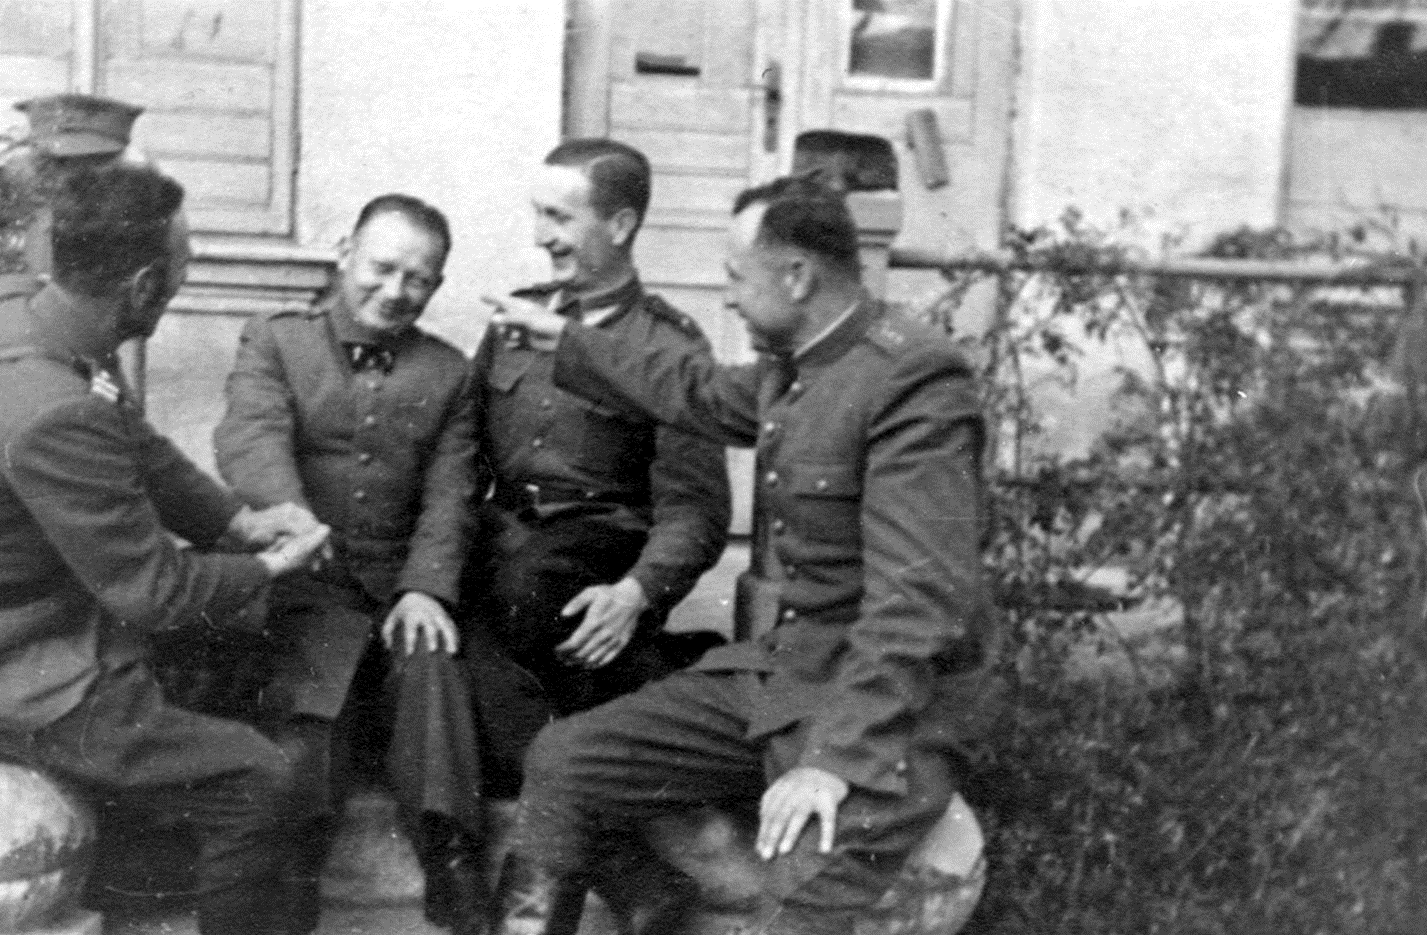
\includegraphics[width=0.7\textwidth]{photo/benedykt_swierczynski_wojna_2.jpg}
\caption[Benedykt Świerczyński z ks. Łopacińskim i rosyjskim kapitanem]{Na zdj.Benedykt Świerczyński z ks. Łopacińskim i rosyjskim kapitanem}
\end{center}
\end{figure}

Po krótkim pobycie \textbf{w Puławach} ruszył pułk Taty na północ i przez Wisłę na sławny przyczółek mostowy \textbf{pod Warką i Magnuszewem}. Tam \textbf{pod Studziankami zginął Francik Kępa z Łagiewnik Wielkich}.Nasz dzielny wojak otrzymuje rozkaz wyjazdu \textbf{do Lublina} po uzupełnienia. Przyprowadził stamtąd po trzech dniach marszu już \textbf{do Nowego Rembertowa pod Warszawą} 240 żołnierzy zamiast 300, z którymi wyszedł z Lublina. Reszta po prostu poszła do lasu. Tu trzy miesiące przepędził na szkoleniu kadry podoficerskiej. \textbf{W tym Rembertowie ożenił się Rudolf Juzek i tutaj też otrzymał nasz Tato ów Krzyż Walecznych oraz drugą gwiazdkę, czyli awans na porucznika.} 

\begin{figure}[!h]
\begin{center}
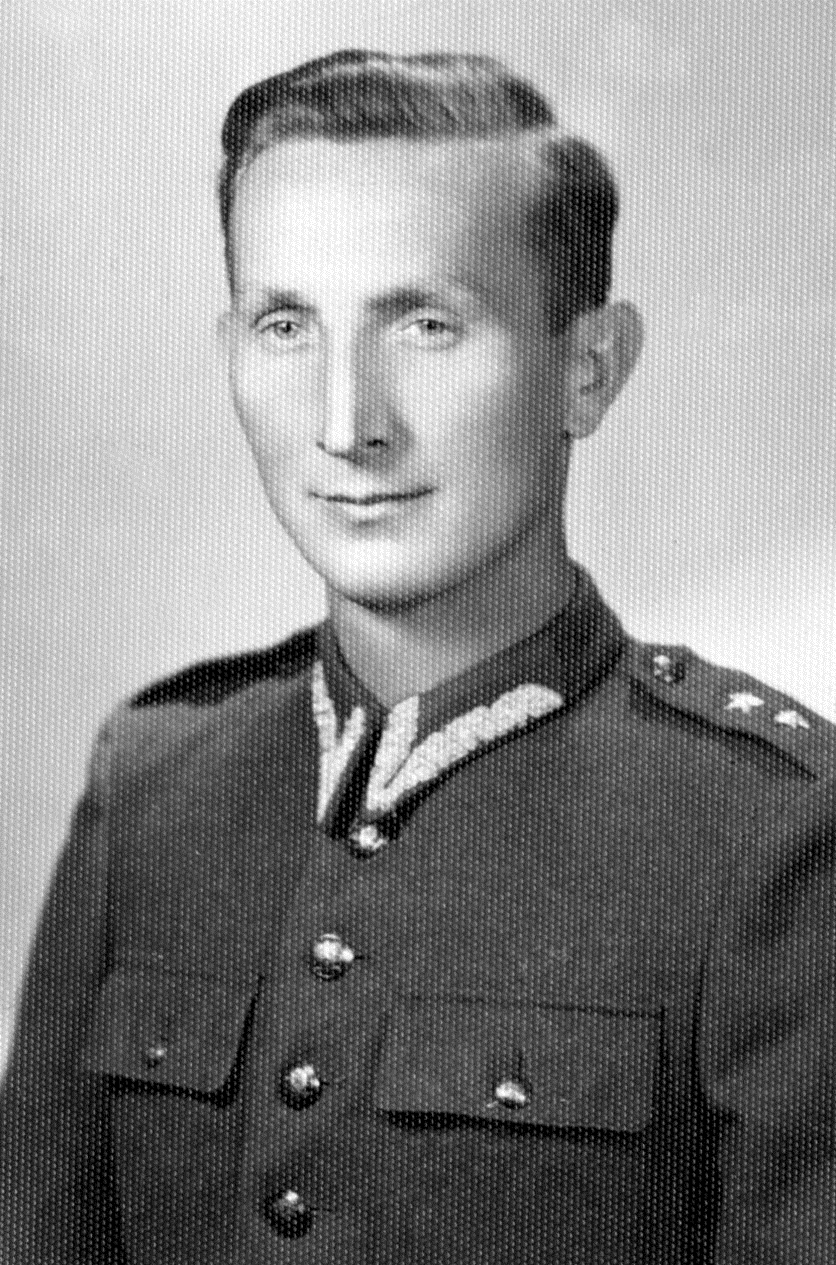
\includegraphics[width=0.35\textwidth]{photo/benedykt_swierczynski_wojna_3.jpg}
\caption[Benedykt Świerczyński w mundurze oficerskim]{Na zdj. Benedykt Świerczyński w mundurze oficerskim}
\end{center}
\end{figure}

W związku z tym awansem został przeniesiony do niespokojnego - frontowego 4 pułku, który stał nad samą Wisłą. Mieszkał wtedy do końca grudnia 1944 r. \textbf{w Aninie z por. Rybaczonkiem} – wspaniałym człowiekiem z Wileńszczyzny. Przeżyli tam wspólnie Święta Bożego Narodzenia, tym okazalsze, że otrzymał paczkę od Janiny Łańcuckiej z Chełma. Wkrótce po Świętach \textbf{opuścili gościnny Anin i wyruszyli nad samą Wisłę}, a sztab pułku był w budynkach administracji \textbf{cmentarza na Bródnie}. Stamtąd z 15 na 16 stycznia ruszyła przeprawa na drugi brzeg Wisły,\textbf{ do zrujnowanej przez hitlerowców Warszawy Lewobrzeżnej}. Wykurzyli Niemców z ich pozycji i zobaczyli jak sobie urządzili ziemianki kradzionymi z opuszczonych mieszkań warszawskich dywanami, fotelami, stołami, obrazami w złoconych ramach. Cóż za kultura u tych „kulturträgerów” (tak skwitował Niemców wasz Dziadek w swym pamiętniku). Po wyzwoleniu Warszawy sztab ich zamieszkał w budynkach administracji \textbf{cmentarza na Powązkach}. 

\textbf{Tymczasem zagony pancerne marszałka Koniewa wyzwoliły Kraków i Częstochowę. W nocy telefon od Szubicza, że Lubliniec wyzwolony!} Następnego dnia udział w historycznej defiladzie w zburzonej Warszawie i świąteczny obiad a na wieczór wiadomość, \textbf{że gen. Zawadzki wyjeżdża na Śląsk wraz z grupą operacyjną, do której zaliczono też naszego Ojca}. Więc wyjazd do sztabu armii \textbf{pod Bydgoszcz}, stamtąd \textbf{z powrotem do Warszawy i do Lublina}, gdzie formowała się owa grupa operacyjna na Śląsk. Tu już gen. Zawadzkiego nie zastał, \textbf{więc drugim rzutem z płk. Ziętkiem i Leonem Fojcikiem przez Staszów do Krakowa}. 

\begin{figure}[!h]
\begin{center}
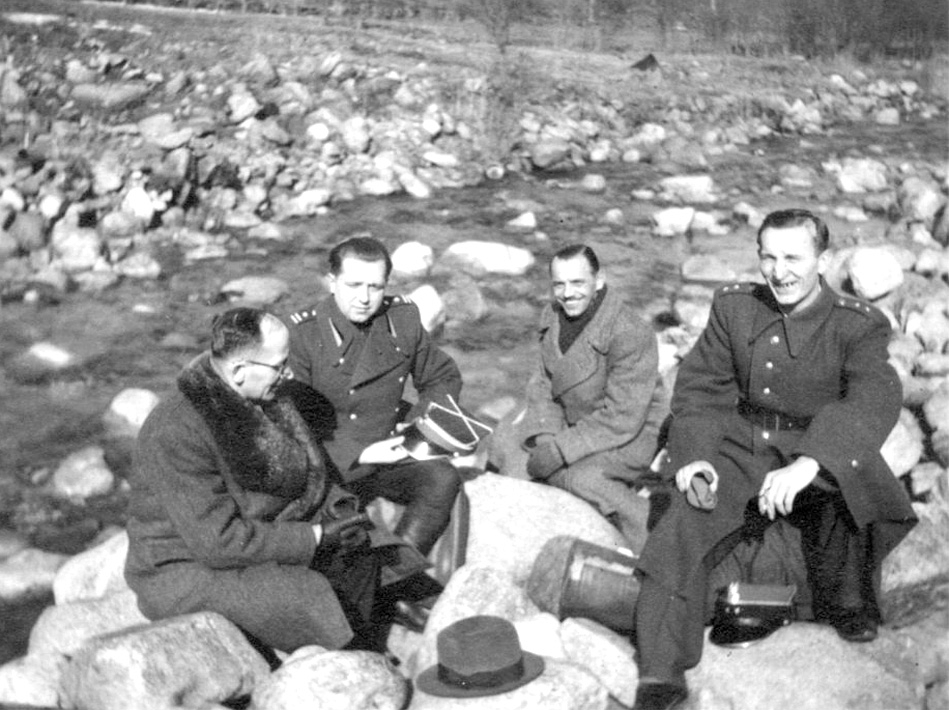
\includegraphics[width=0.6\textwidth]{photo/benedykt_swierczynski_leon_fojcik.jpg}
\caption[Benedykt Świerczyński z Leonem Fojcikiem]{Na zdj. Benedykt Świerczyński z Leonem Fojcikiem}
\end{center}
\end{figure}

Następnego dnia - \textbf{27 stycznia rankiem byli już w Katowicach!} W kwaterze przy ul. Rybnickiej powitał ich kpt. \textbf{Stanisław Mrowczyk}, który do rana następnego dnia dał im wolną rękę. Więc nasz Tato ruszył \textbf{pieszo do rodziny swego brata Józefa na Ligotę}.

Na tym urywa się pamiętnik naszego Taty. Nasza Mama nieroztropnie puściła unikalny rękopis do czytania w rodzinie, zamiast zrobić przynajmniej jedną kserokopię. Wrócił do nas ów pamiętnik mocno okrojony, bo przecież nasz Tato obiecywał opisać swe dzieje aż do czasów nam współczesnych. Kończy się on w pół słowa na 28 stycznia 1945 r., a więc jeszcze przed końcem wojny. Szkoda też, że okazałem się jednym z ostatnich, którzy dostąpili łaski oglądania oryginału, już wtedy niestety kończącego się na stronie 257. Od razu też go wówczas skserowałem, i zrobiłem parę kserokopii dla rodziny. Jeśli u czytelników tej historii rodziny Świerczyńskich i Wilczków gdzieś zawieruszyła się dalsza część pamiętnika mojego Taty, niech ją zwróci, np. pocztą bez podawania nadawcy, nawet gdyby był on mocno poplamiony, przyniszczony. Będę się modlił za tego, kto odda ów rękopis, nawet gdyby się nie ujawnił...

Jakiż to musiał być awans i radość waszego Dziadka, gdy wrócił w swoje rodzinne strony w mundurze oficerskim, gdy go już pewnie mieli za zaginionego, bo przecież listów nie mógł pisać do domu, gdy znalazł się w niewoli sowieckiej, a zwłaszcza gdy znalazł się w Wojsku Polskim i bił Niemca na froncie wschodnim. Teraz jako kandydat do ręki ślicznej Wilczkówny stał się partią nie do odrzucenia.

\begin{figure}[!h]
\begin{center}
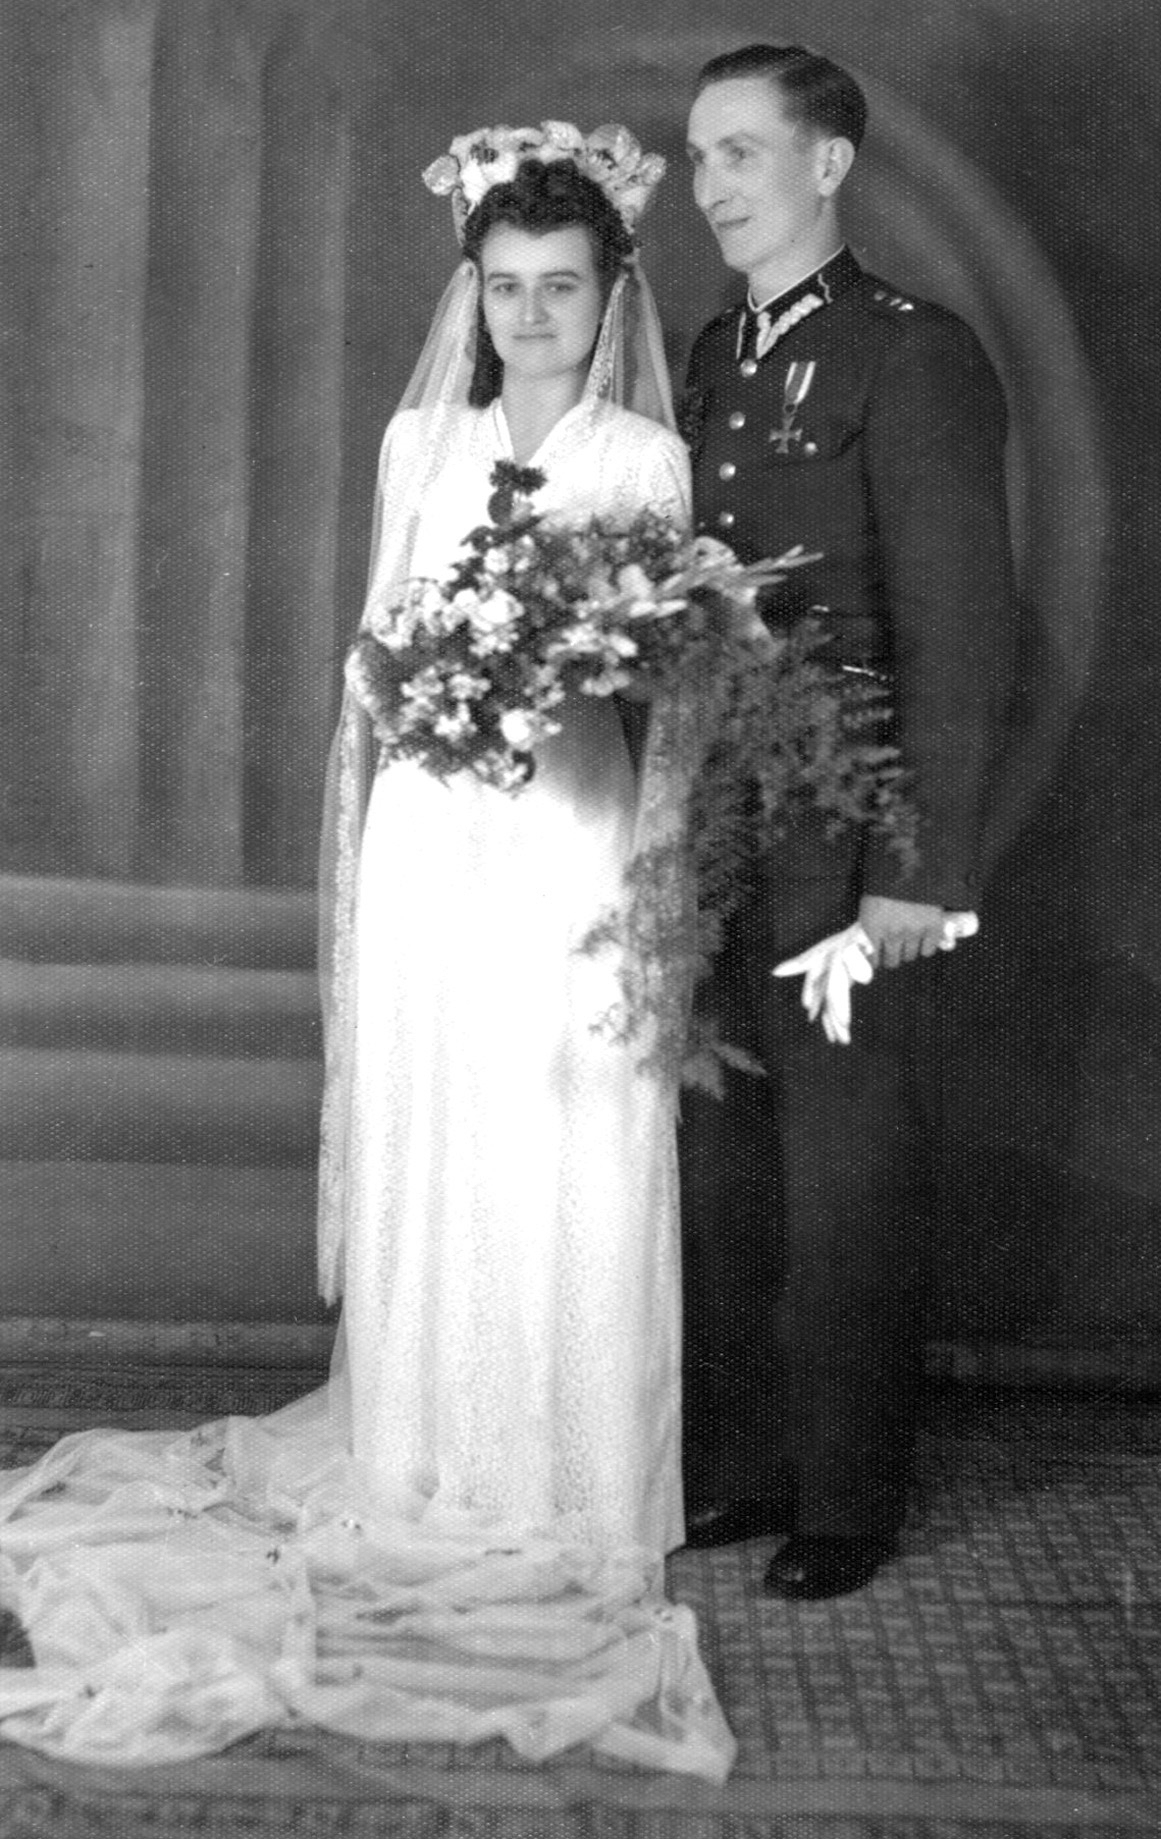
\includegraphics[width=0.4\textwidth]{photo/benedykt_radegunda_swierczynscy_slub.jpg}
\caption{Ślub Radegundy Wilczek i Benedykta Świerczyńskiego}
\end{center}
\end{figure}

\begin{sidewaysfigure}[!hp]
\begin{center}
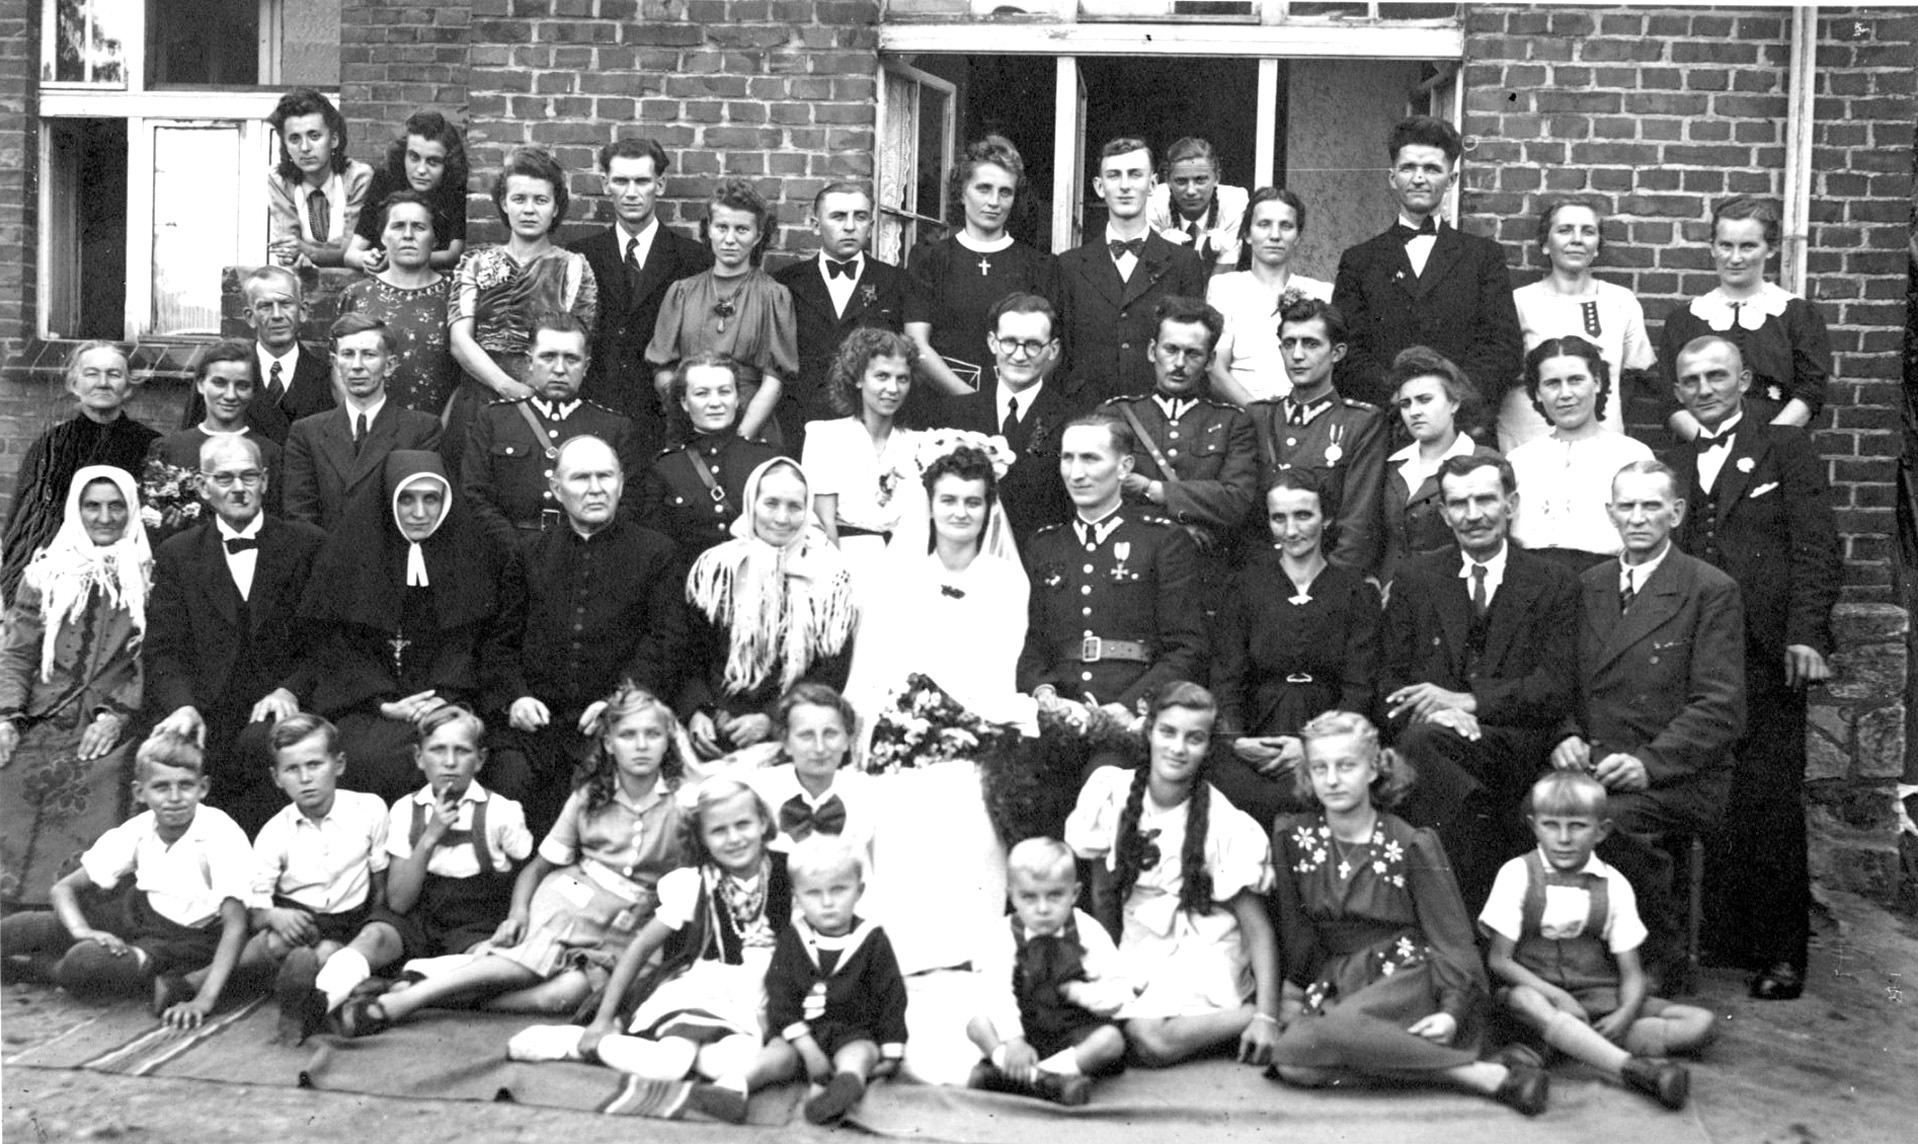
\includegraphics[height=120mm]{photo/benedykt_radegunda_swierczynscy_slub_2.jpg}
\caption[Ślub Radegundy i Benedykta Świerczyńskich - zdjęcie zbiorowe]{Na zdjęciu od lewej siedzą na kocach: Antoś Wilczek, Heniu Kochel, Maryś Jasak, Basia Wilczkówna, obok Ela Świerczyńska, przed nią Marysia Wilczkówna, obok Gutek Lehman, po drugiej stronie sukni ślubnej Panny Młodej Jasiu Wilczek, za nim Bronia Wilczkówna, obok Ela Wiora i Tadek Lehman. Siedzą na krzesłach od lewej: praprababcia Franciszka Jerominek, pradziadek Tomasz Wilczek, siostra Aurelia Świerczyńska, ks. prob. X. Dwucet, prababcia Eufemia Świerczyńska, Radegunda Wilczek-Świerczyńska, Benedykt Świerczyński, prababcia Zofia Wilczek, pradziadek Edward Świerczyński i NN. W trzecim rzędzie stoją od lewej Anna Wiora (z domu Wilczek), Maria Jerominek (siostra prababci Zofii), Paweł Wiora, Leon Fojcik, Eleonora Kościuszko Fojcik, pp. Rożniewscy, NN, Rudolf Juzek, Irena Juzek, Wanda Kochel, Ludwik Jerominek. W czwartym rzędzie stoją od lewej: Edmund Wilczek (brat Tomasza), NN, Paweł Jerominek z Żoną, Janina Wiora, Edward Otto, Rózia Świerczyńska, Walerian Wilczek, Gertruda Kukowka (siostra Marii Jerominek), Wiktor Kukowka, Antonina Otto (siostra Edwarda Otto) i NN. Na murku oparte i w oknie NN.}
\end{center}
\end{sidewaysfigure}

Musieli jednak ze ślubem zaczekać aż do powrotu z Niemiec waszego pradziadka Tomasza, a ojca waszej Babci.\textbf{Mogli się pobrać dopiero 18 września 1945 r. w kościele pw. św. Mikołaja w Lublińcu. Wesele odbyło się w domu Panny Młodej przy ul. Opolskiej. Niestety, następnego dnia wasz pradziadek Edward zmarł chyba na zawał serca}, mimo że przy nim była znakomita pomoc medyczna – jego córka Anastazja (siostra Aurelia).

Karierę zawodową rozpoczął nasz Tato \textbf{od Urzędu Wojewódzkiego w Katowicach}, w którym został zatrudniony \textbf{1 lutego 1945 r.} i pracował tam do \textbf{15 lutego 1948 r.} Nasza Mama mówiła, że zwolnili go za to, iż starał się o zwolnienie z więzienia swego szwagra Antoniego Lehmana, którego ówczesne władze uważały za Niemca (nazwisko niemieckie oraz służba w Wehrmachcie, a także figurowanie na volksliście wystarczyło). 16 lutego podjął pracę w Centrali Zbytu Węgla na dobrze płatnym stanowisku, z którego wygryzła go w 1951 r. jakaś Żydówka. To był pechowy rok dla naszej rodziny: zmarła bowiem 10 stycznia babcia Eufemia, i jeszcze to zwolnienie Taty. Znalazł pracę w WPHW na stanowisku sprzedawcy w sklepie sportowym przy ówczesnej ulicy Wieczorka (dziś i przed wojną Staromiejska) z lichą płacą. \textbf{21 kwietnia 1952 r. został dyrektorem w Zakładach Drzewnych podległych Katowickiemu Zjednoczeniu „Prodryn”. Pracował tam do 30 czerwca 1956 r.} Nie wiem dlaczego Tato odszedł stamtąd i zatrudnił się w Zakładach Mięsnych w Mysłowicach, gdzie licho zarabiał, mimo że pełnił tam funkcję dyrektora, ale otrzymywał tam ekwiwalent mięsny, dzięki czemu mogliśmy się do woli obżerać mięsem, z którego nasza Mama potrafiła wyczarowywać kulinarne cudeńka. \textbf{Tak było do 31 grudnia 1957 r.}, kiedy to naszego Tatę zatrudnił jego serdeczny przyjaciel z czasów wojny - płk. Bronisław Szubicz, dowódca Jednostki Wojskowej stacjonującej w Katowicach między ulicą Raciborską (w PRL-u ul. Świerczewskiego), ul. Bpa Adamskiego i ul. Koszarową. \textbf{Tam pracował do 15 lipca 1959 r.} Gdy byłem w prewentorium w Zakopanem wiosną 1958 r. przyjechał do mnie z moimi rodzicami i bardzo dobrze go stamtąd wspominam.
\begin{figure}[!h]
\begin{center}
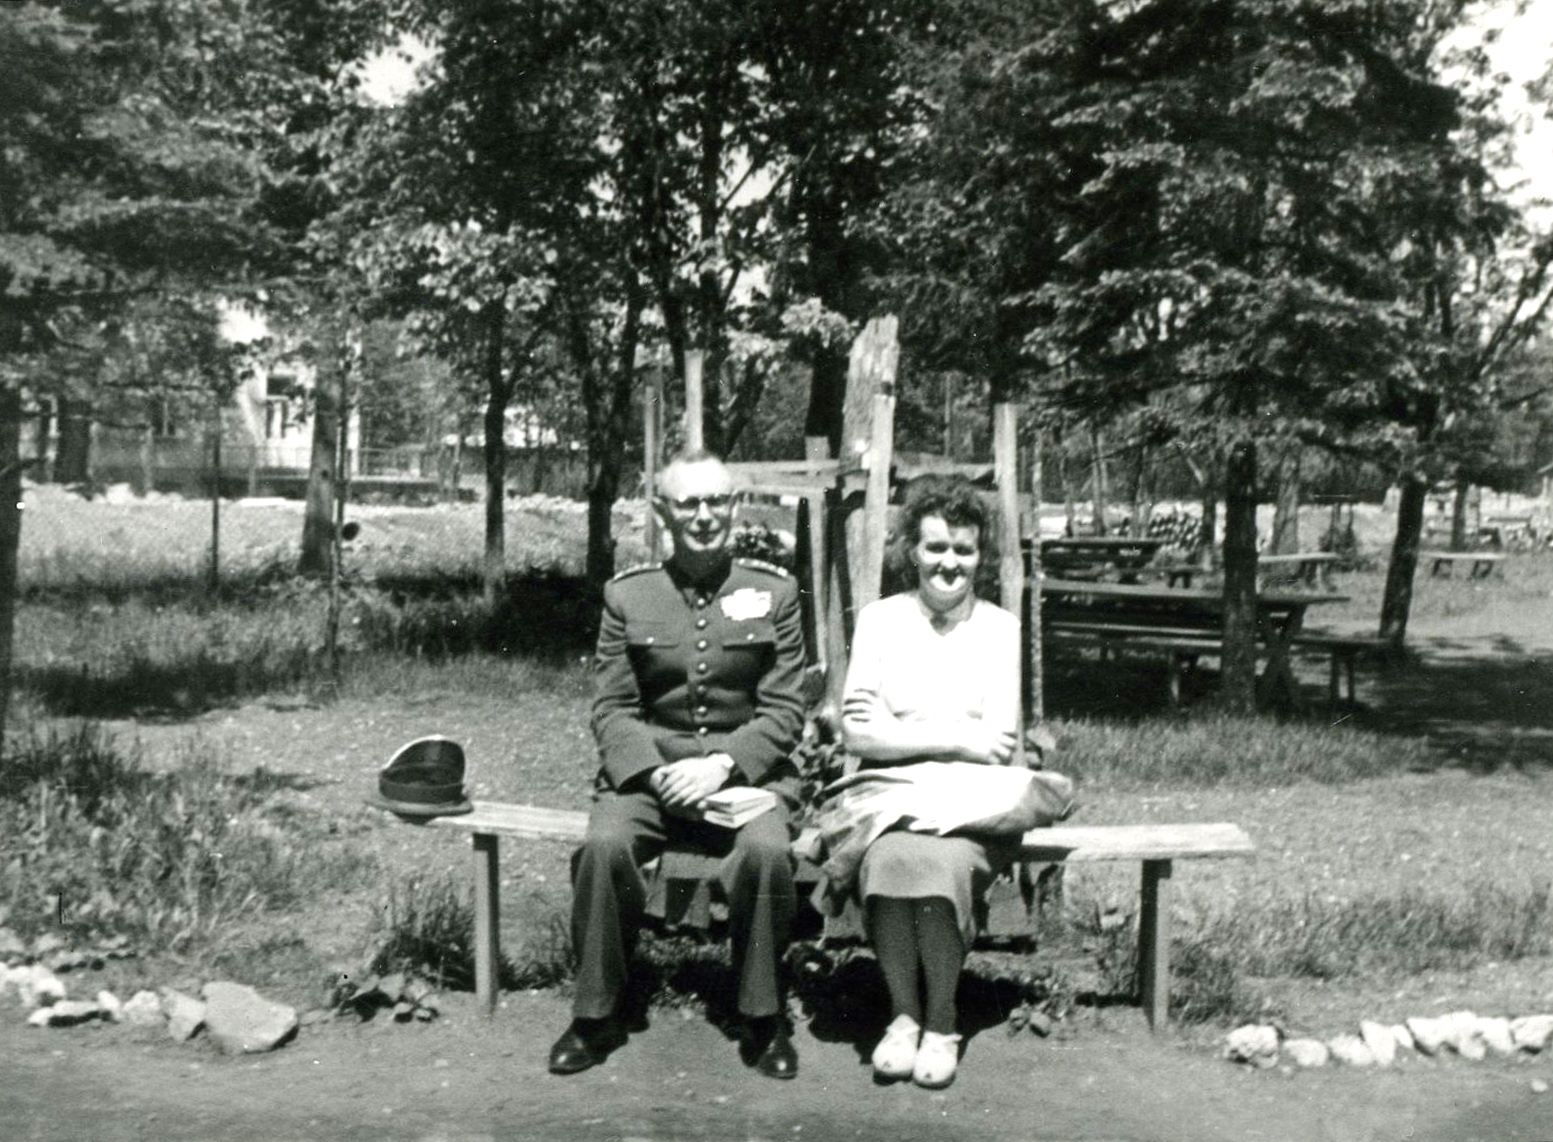
\includegraphics[width=0.65\textwidth]{photo/radegunda_swierczynska_plk_szubicz.jpg}
\caption{Na zdj.babcia Radegunda z płk. Szubiczem}
\end{center}
\end{figure}

Tymczasem kolejny serdeczny przyjaciel naszego Taty – \textbf{Rudolf Juzek, będący do tej pory dyrektorem Zarządu Wojewódzkiego Ligi Przyjaciół Żołnierza awansował aż na stanowisko sekretarza Komitetu Wojewódzkiego PZPR}. Wprowadził on więc naszego Tatę na swe dotychczasowe stanowisko \textbf{dnia 16 lipca 1959 r.}
\begin{figure}[!h]
\begin{center}
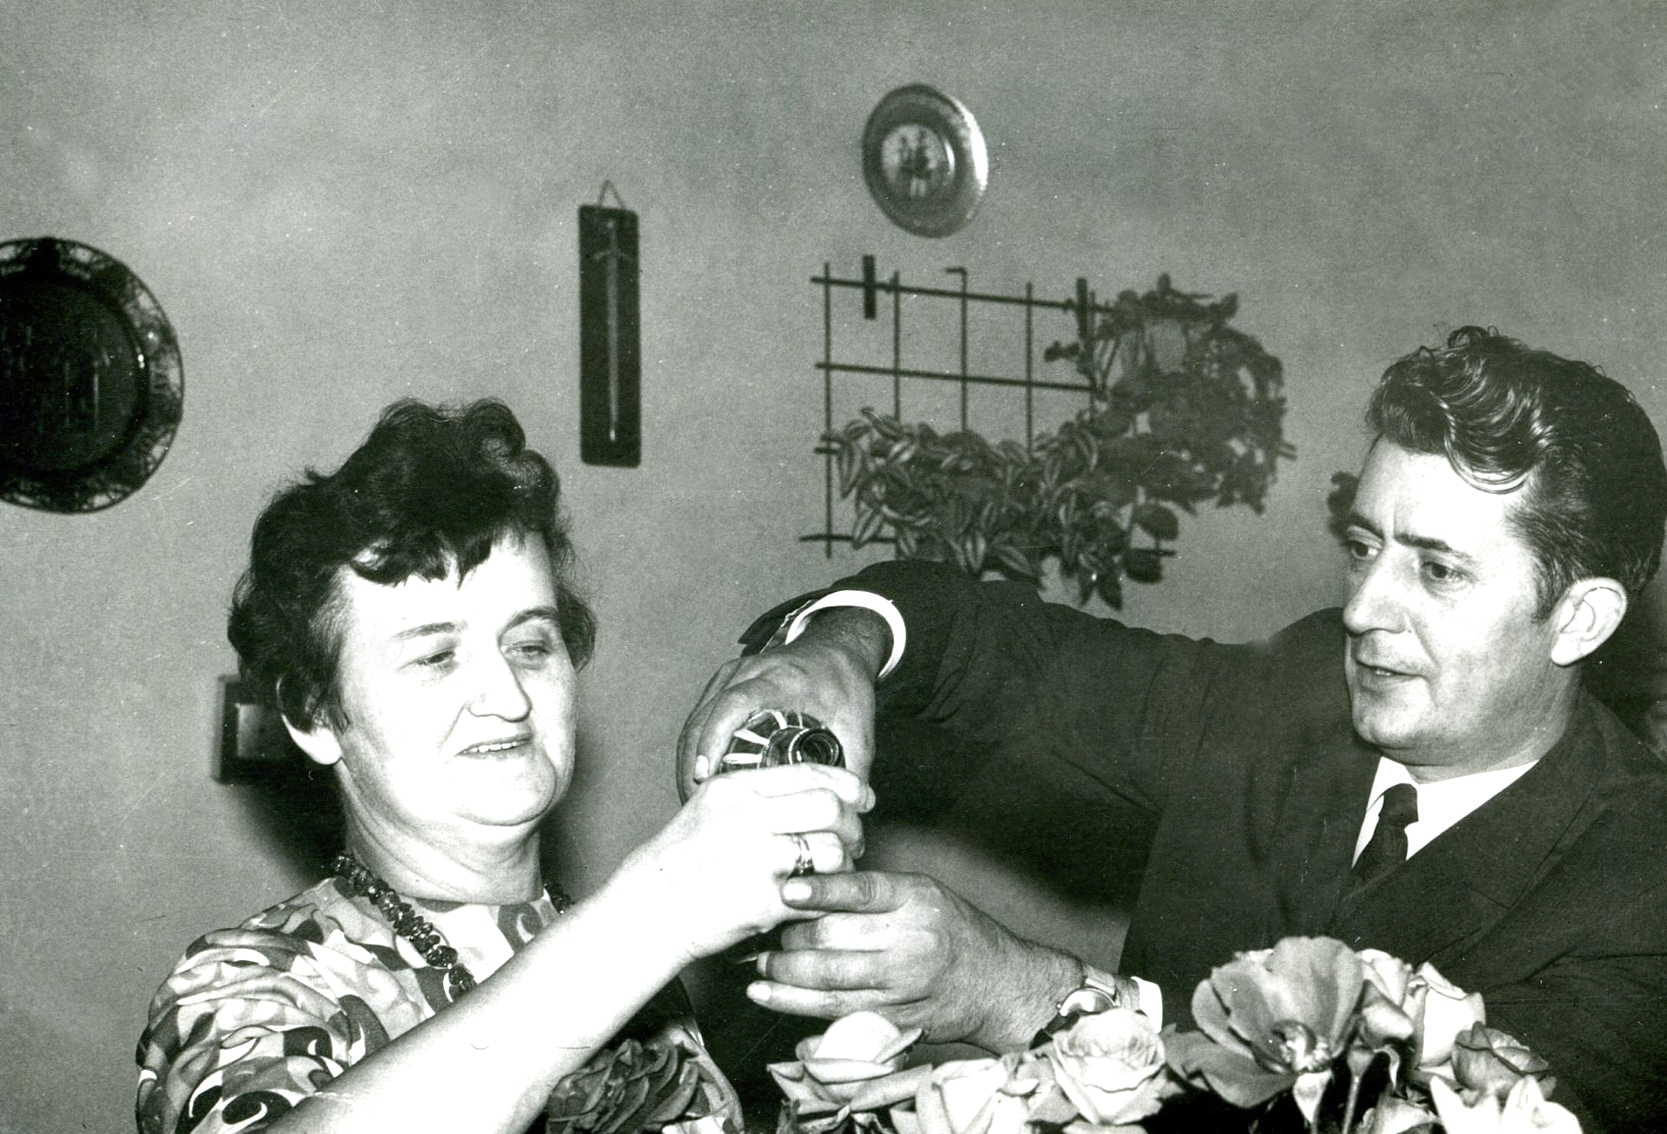
\includegraphics[width=0.65\textwidth]{photo/radegunda_swierczynska_rudolf_juzek.jpg}
\caption[Radegunda Świerczyńska i Rudolf Juzek]{Na zdj. Radegunda Świerczyńska i Rudolf Juzek}
\end{center}
\end{figure}

Z tą instytucją paramilitarną związał się nasz Tato na długo, do emerytury, a nawet jeszcze dłużej, gdy pobierał już świadczenia emerytalne, \textbf{aż do początku lat 90’}. Wypada więc parę słów powiedzieć o Lidze Przyjaciół Żołnierza, która powstała w 1953 r. z połączenia Ligi Morskiej z Ligą Lotniczą. Wtedy prezesem był X. \textbf{Stańczyk}. Natomiast wiceprezesem był aktualnie urzędujący dyrektor Ligi. Po Stańczyku prezesem był X. \textbf{Gorczyca} -- I zastępca przewodniczącego Wojewódzkiej Rady Narodowej, który był bardzo przemądrzały i truł zdrowie naszemu Tacie. Po nim prezesem był \textbf{gen. Roczniok} – przyjaciel naszego Taty, który bywał w naszym mieszkaniu.
\begin{figure}[!h]
\begin{center}
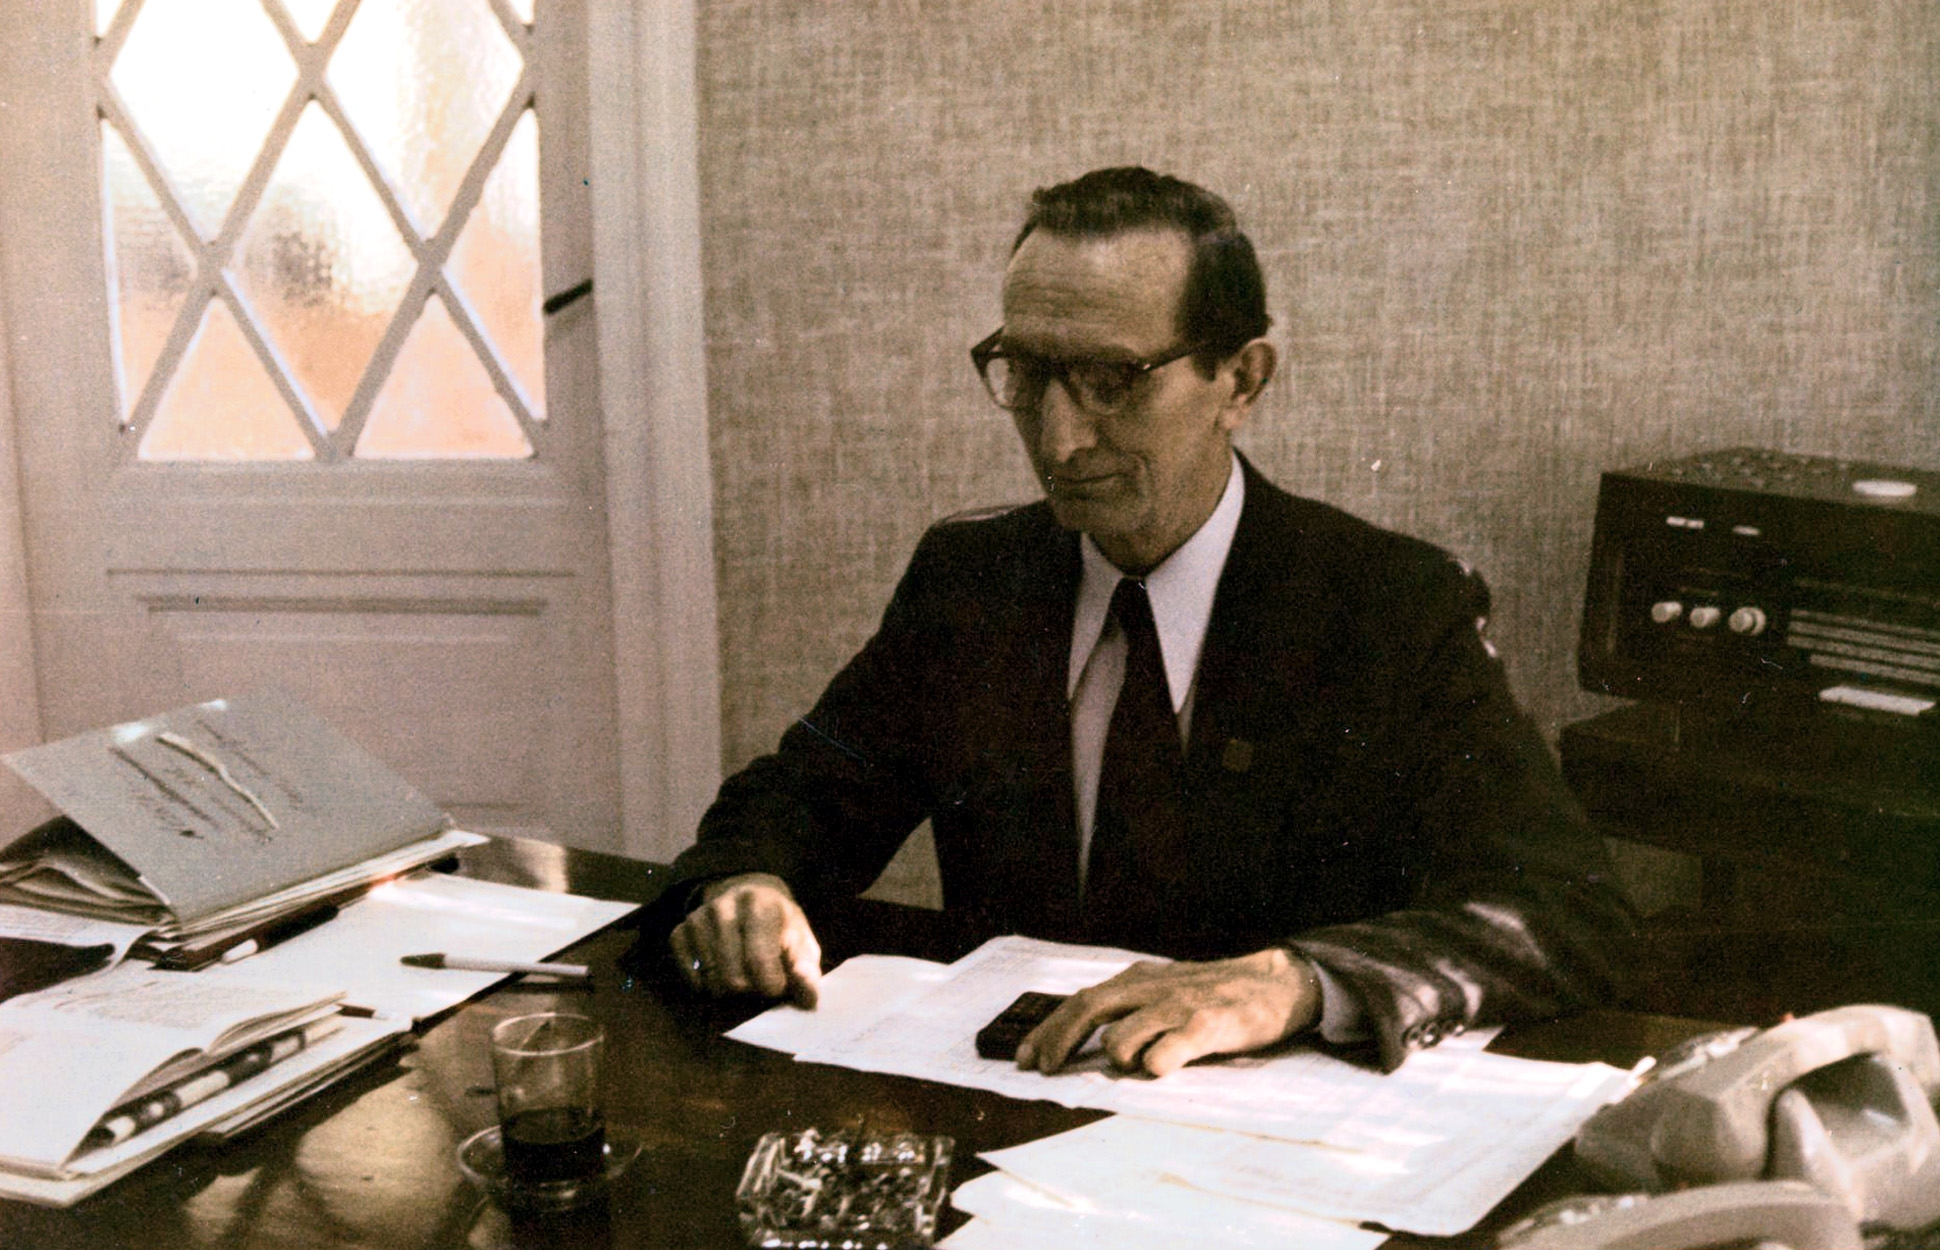
\includegraphics[width=0.7\textwidth]{photo/benedykt_swierczynski_1979.jpg}
\caption[Benedykt Świerczyński przy dyrektorskim biurku w 1979 r.]{Na zdj. Benedykt Świerczyński przy dyrektorskim biurku w 1979 r.}
\end{center}
\end{figure}

Kolejnym prezesem był \textbf{gen. Mateja}, szef sztabu wojewódzkiego. Chciał on się pozbyć ze sztabu pułkownika Wołyńskiego i upatrzył dla niego stanowisko dyrektora LOK-u. Tak więc spowodował on odwołanie Benedykta Świerczyńskiego z funkcji dyrektora i powołanie pułkownika Wołyńskiego. Pamiętamy z tamtego czasu wielu współpracowników naszego Taty, zwłaszcza przemiłego pana z muszką – \textbf{Mieczysława Paździerskiego}, który był jego kierowcą.

Częstymi gośćmi przy okazji urodzin Taty byli państwo \textbf{Zofia i Witold Szmiglowie} (pani Zofia była kadrową i pracowała od 1954 r. w LPŻ) oraz państwo \textbf{Róża i Bolesław Pawlusowie} z Bielska Białej (byli także na pogrzebie Taty), oraz państwo \textbf{Janina i Józef Góreccy} (pani Janina organizowała wycieczki zagraniczne dla pracowników LPŻ, późniejszego LOK-u dzięki czemu nasi rodzice, nierzadko  w towarzystwie naszych krewnych, byli chyba we wszystkich krajach tzw. demokracji ludowej).
\begin{figure}[!h]
\begin{center}
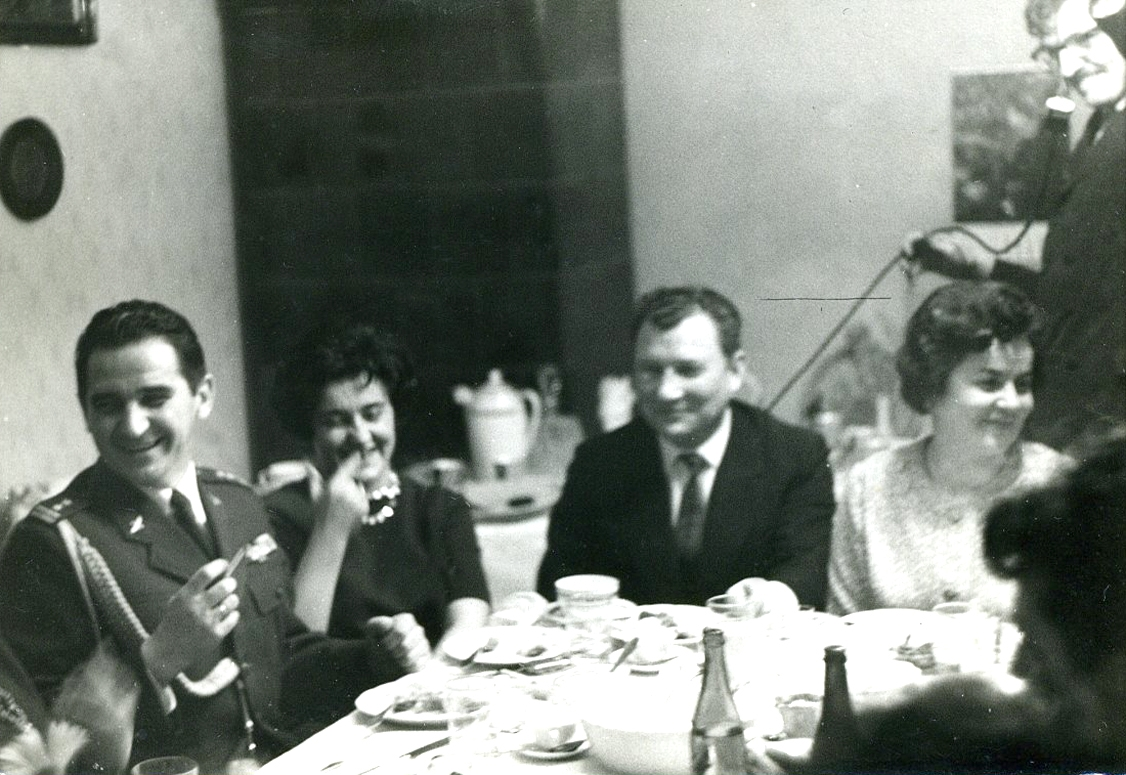
\includegraphics[width=0.7\textwidth]{photo/szmiglowie.jpg}
\caption[Państwo Szmiglowie]{Na zdj. Państwo Szmiglowie pomiędzy pułk. oraz p. Adą Golową.}
\end{center}
\end{figure}

Najczęstszym jednak gościem był pan \textbf{Rudolf Juzek}, który przychodził na niejedną partyjkę szachów. Każdego roku nasi rodzice wyprawiali urodziny, co było okazją do większych lub mniejszych zjazdów rodzinnych. Największe oczywiście były na tzw. „Abrahama” (czyli 50’ urodziny) oraz na srebrne i złote gody. Nasza Mama świetnie gotowała, ale zawsze na taką wielką uroczystość któraś z cioć przyjeżdżała do pomocy. Ponieważ nasz Tata, do czasu objęcia stanowiska dyrektora LPŻ, nie zarabiał dobrze, nasza Mama szyciem dorabiała większe pieniądze. 














\clearpage
\section{Życie Czesława Michała}
Pierworodnym ich synem jest \textbf{Czesław Michał Świerczyński} -- autor niniejszej historii rodu Świerczyńskich i Wilczków – \textbf{urodzony 16 września 1946 r. w Katowicach w mieszkaniu przy ul. wówczas Wandy}, a od późnych lat 40’ ul. Marii Skłodowskiej Curie.
\begin{figure}[!h]
\begin{center}
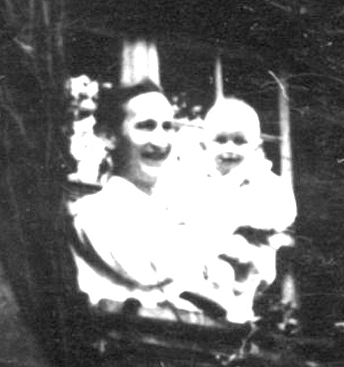
\includegraphics[width=0.4\textwidth]{photo/czeslaw_swierczynski_roczek.jpg}
\caption[Maleńki Czesiu Świerczyński u taty na rękach]{Na zdj. maleńki Czesiu Świerczyński u taty na rękach}
\end{center}
\end{figure}

Było to mieszkanie po pani \textbf{Kapinos}, która otrzymała w tej samej klatce schodowej mniejsze mieszkanie. Często też bywała u nas i nami się opiekowała. W jej rodzinie był ksiądz, który też nieraz bywał u nas i częstował nas czekoladami, co w tamtych czasach było rarytasem. \textbf{W tym mieszkaniu przyszedł na świat 25 lutego 1948 r. mój brat Józef Tomasz Świerczyński.}
\begin{figure}[!h]
\begin{center}
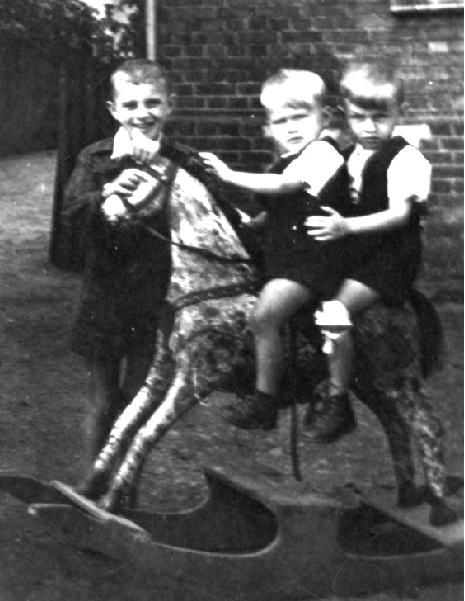
\includegraphics[width=0.4\textwidth]{photo/jozef_tomasz_swierczynski.jpg}
\caption[Józef Tomasz Świerczyński na koniu bujanym]{Józef Tomasz Świerczyński (na koniu bujanym) wraz z bratem Czesławem oraz wujkiem Jankiem Wilczkiem.}
\end{center}
\end{figure}

\textbf{25 grudnia 1952 r. przyszła na świat nasza siostrzyczka – Janina Zofia, która niestety już 22 stycznia 1953 r. zmarła.}

Obaj chodziliśmy do tej samej chłopięcej Szkoły Podstawowej Nr 30, której budynek łączył się ze szkołą podstawową dla dziewcząt (ale był odgrodzony) i Liceum im. Marii Konopnickiej. Budynek tej naszej szkoły sąsiadował przez ulicę z kościołem parafialnym pw. św. ap. Piotra i Pawła. Ani ja ani mój brat Józiu nie byliśmy tam orłami. Gdy dzięki towarzystwu znakomitego ucznia z Warszawy – Tadka Wasiutyńskiego i Jurka Dymnego zacząłem się wznosić na wyżyny, zapadłem na jakąś chorobę płuc i wylądowałem w piątej klasie na pół roku w Prewentorium „Oaza” w Zakopanem, gdzie rozleniwiłem się doszczętnie, bo tam dbano jedynie o zdrowie małych pacjentów, a nie o wyniki w nauce.
\begin{figure}[!h]
\begin{center}
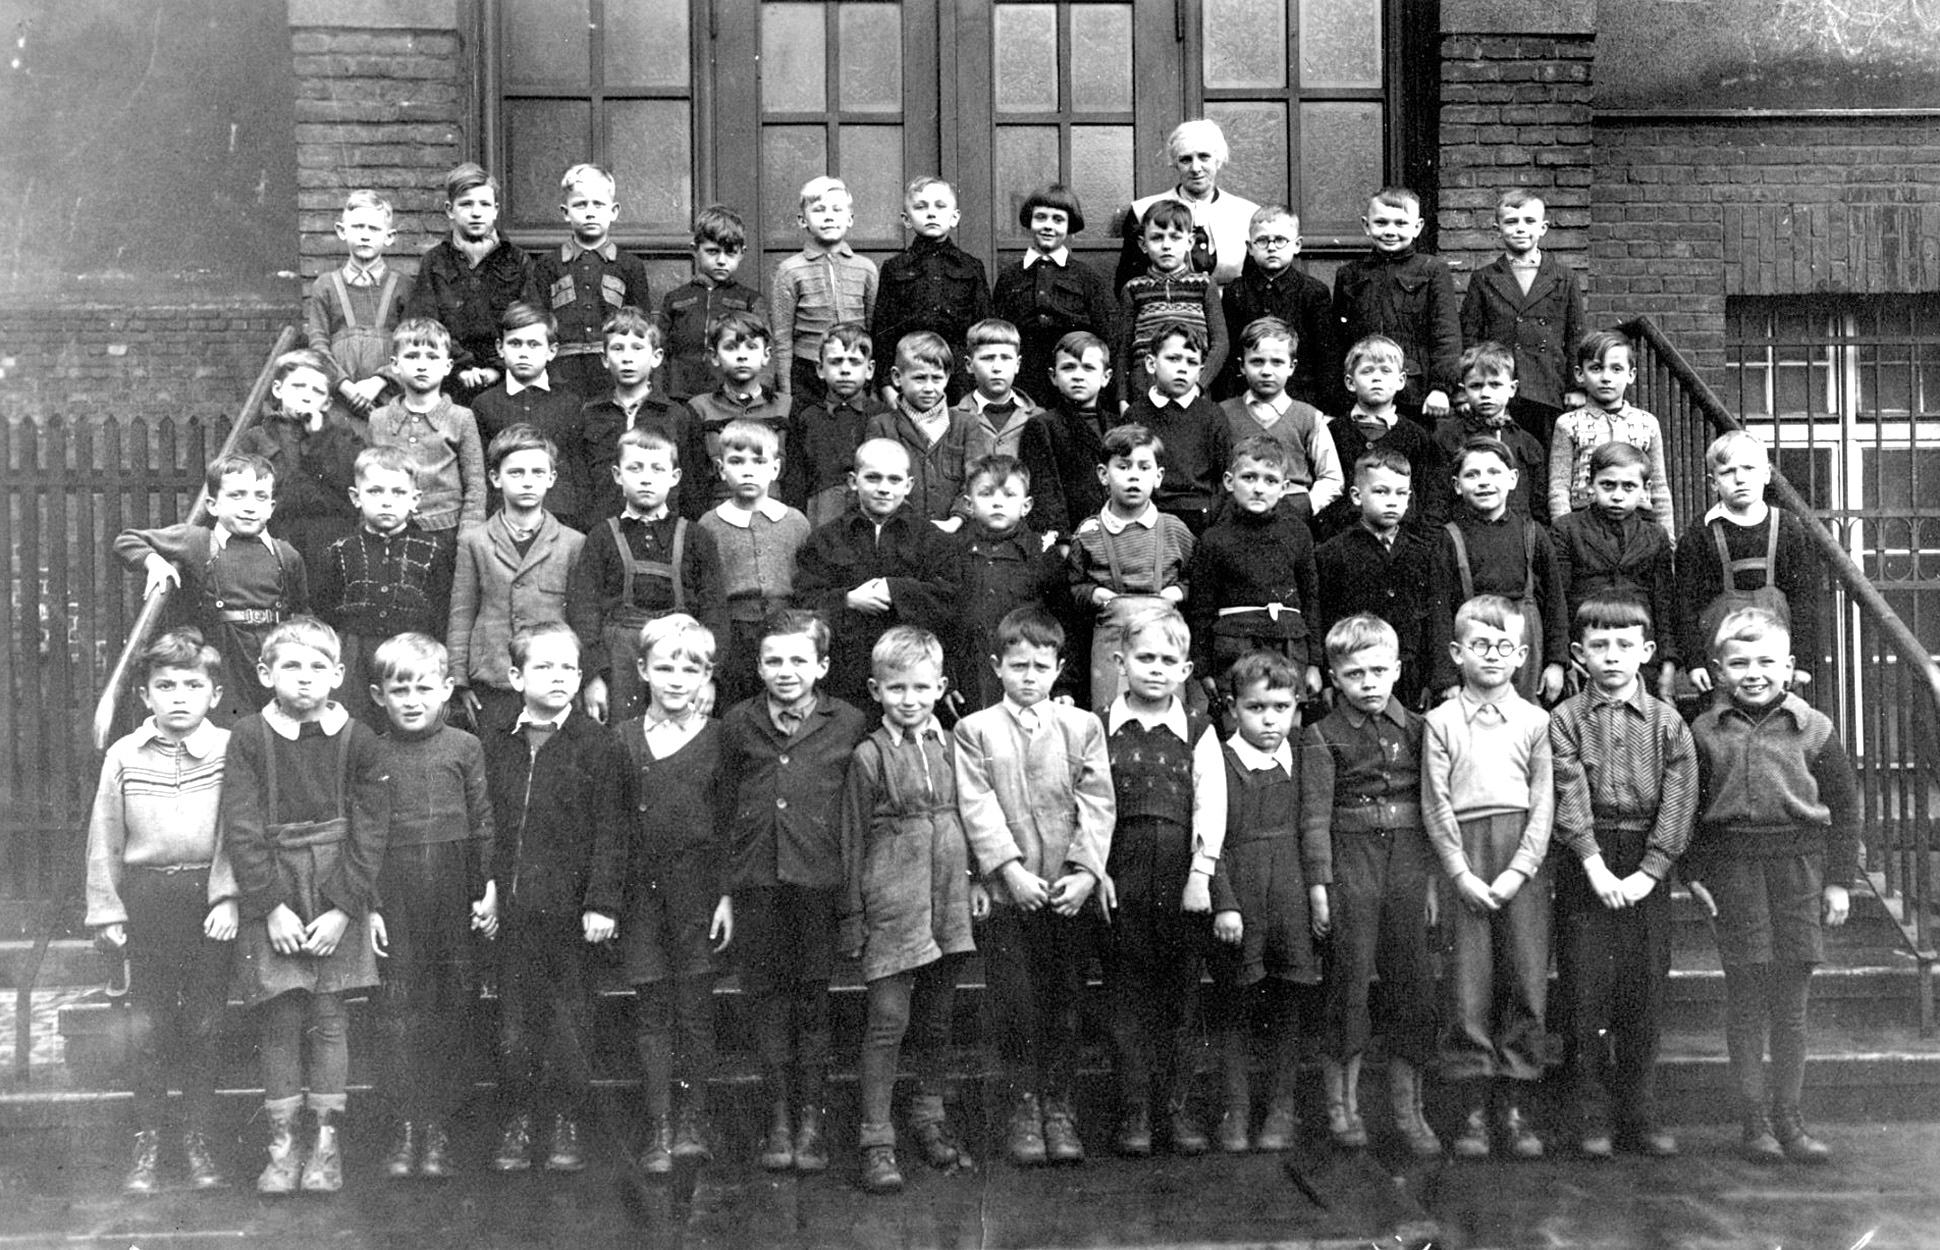
\includegraphics[width=\textwidth]{photo/czeslaw_swierczynski_i_kl_sp.jpg}
\caption[Zdjęcie zbiorowe I kl. SP]{Zdjęcie zbiorowe I kl. SP - Czesław Świerczyński w ostatnim rzędzie, za nim wychowawczyni Piaskowska}
\end{center}
\end{figure}

Gdy tak rozleniwiony wróciłem do swojej – już wówczas szóstej klasy od razu spadłem na sam dół tabeli i tak zostało do końca siódmej klasy. Ojciec mój, wówczas już dyrektor Zarządu Wojewódzkiego LPŻ zabrał mnie do psychologa (co na ówczesne czasy było ewenementem), by ten orzekł do jakiej szkoły najlepiej się nadaję. Ów psycholog, przed którym otwarłem wówczas swoją duszę (m.in. wyznałem, że chciałbym zostać pisarzem – co później mój Tato wiele razy przypominał na forum rodzinnym – by moim kosztem bawić towarzystwo) powiedział przy mnie mojemu Tacie, że nie nadaję się do żadnej szkoły technicznej, zaś najbardziej odpowiada moim zainteresowaniom Liceum Ogólnokształcące. 

Mój Tato wbrew tym sugestiom wysłał mnie do Śląskich Technicznych Zakładów Naukowych, gdzie sobie mnie pokazywano na warsztatach szkolnych jako zupełne beztalencie! Po pierwszym okresie (a wtedy okresów w ciągu roku były cztery) ze wszystkich przedmiotów technicznych i z matematyki miałem oceny niedostateczne, więc poszedłem sam do najbliższego terytorialnie Ogólniaka z zamiarem kontynuowania tam nauki. Trzeba było nadrabiać zaległości programowe, a ponadto bardzo się pilnować i uzupełnić braki z matematyki. Tato sporadycznie kontrolował moje postępy w nauce, sam zaś nie miałem wystarczającej siły woli, by temu wszystkiemu podołać.

Skończyłem rok z dwoma poprawkami (z matematyki i j. rosyjskiego), których nie zdałem, więc powinienem powtarzać klasę, lecz mój ojciec się na mnie tak dalece rozeźlił, że posłał mnie do Zasadniczej Szkoły Górniczej przy Kopalni „Katowice”. To była dla mnie gehenna. Byłem traktowany przez rówieśników, dla których operowanie siekierą, kilofem, młotem i piłą było codziennością, jak jakiś przygłup, niedorajda, którego można sponiewierać, tym bardziej, że się nie umiał bronić. Z tego powodu wagarowałem, że aż ojca wezwali do szkoły. Dopiero w drugiej klasie się opamiętałem i stałem się prymusem, by zapewnić sobie możliwość zdania egzaminu do Technikum Górniczego w Brynowie, które ukończyłem w 1967 r. z przeciętnymi ocenami, więc o studiach nie było co marzyć.
\begin{figure}[!h]
\begin{center}
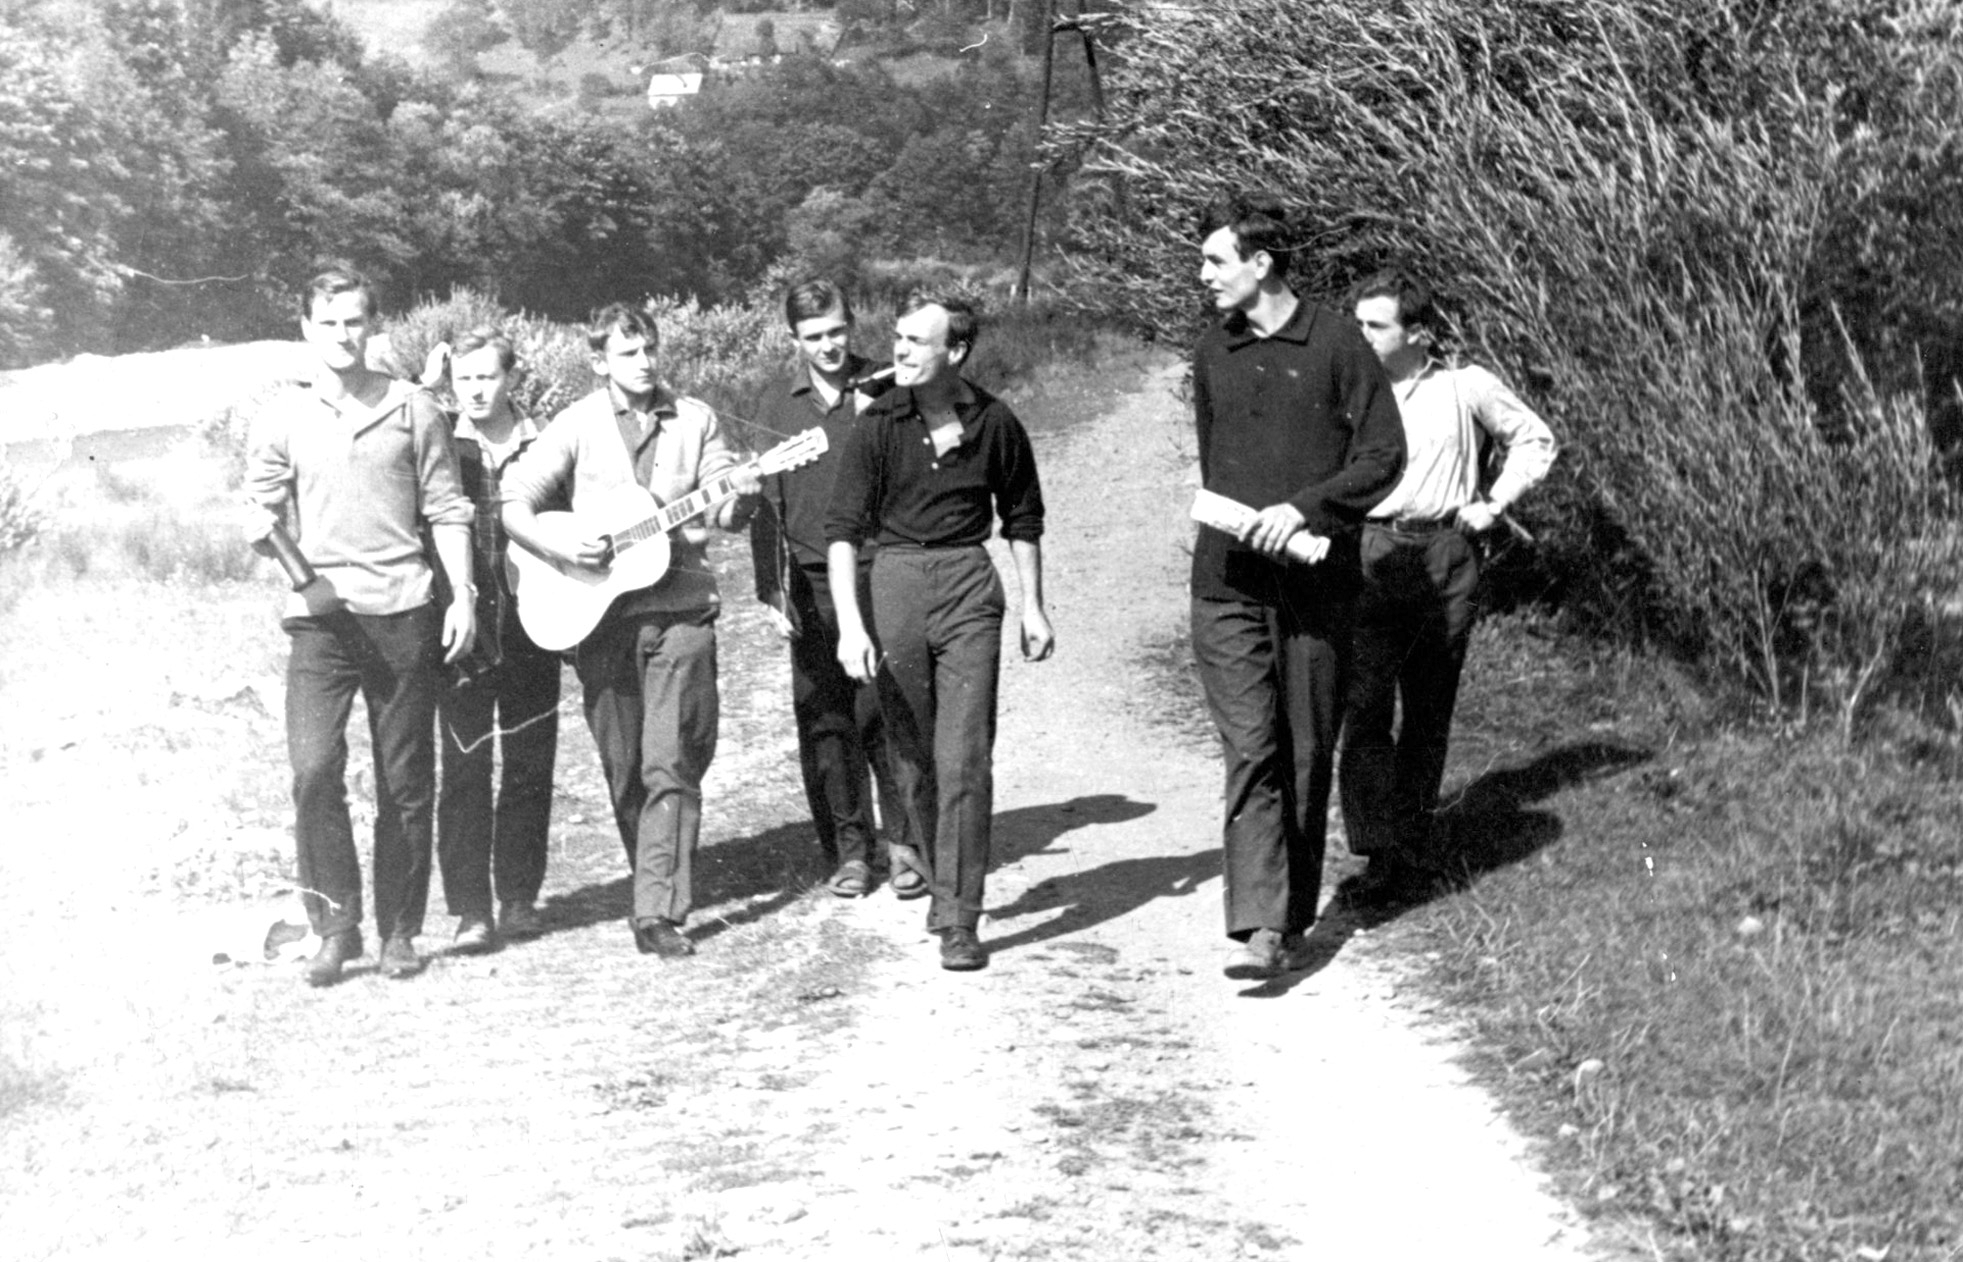
\includegraphics[width=\textwidth]{photo/czeslaw_swierczynski_z_kolegami.jpg}
\caption[Czesław Świerczyński z kolegami]{Na zdj. od lewej X. Foltyn, Eligiusz Błaszczyk, Janusz Mecner, Zbigniew Buzderewicz, Czesław Świerczyński, Y. Szyma, tj.  koledzy z Technikum Górniczego}
\end{center}
\end{figure}

Gdy jednak mój przyjaciel Zbyszek Dziedzina zapowiedział, że startuje na Filologię Polską na nowo tworzonym Uniwersytecie Śląskim, sam też postanowiłem tam wystartować. Start jednak okazał się kompletnym falstartem, gdyż w przeddzień egzaminów wstępnych przyszli do mnie koledzy z technikum, którzy wyszli pierwszy raz na przepustkę z wojska. Skończyło się wielkim kacem. Cóż mądrego można było spłodzić na egzaminie pisemnym?! Tylko dzięki znajomościom Ojca dostałem się na te studia... Tam nareszcie byłem kimś, zwłaszcza po zdanych na piątkę egzaminach z logiki, ze staro-cerkiewno-słowiańskiego języka i gdy z poetyki napisałem jedyną trafną analizę wiersza Przybosia.  Wybrałem temat pracy magisterskiej z językoznawstwa na temat zapowiedników i odpowiedników w zdaniach podrzędnych w języku literackim, mówionym i gwarach. Otrzymałem od mojej pani promotor – prof. Bajerowej entuzjastyczny list, a potem zmiana – ocena tylko dobra i w związku z tym upadła propozycja pracy na uczelni. W rok później obecny prof. Edward Polański zaproponował mi pracę w Katedrze Dydaktyki Języka Polskiego, ale pod namową mojej małżonki nie skorzystałem z tej propozycji i zacząłem wieść żywot niespełnionego naukowca jako belfer i po trosze polityk.

W tym też czasie zgłupiałem do tego stopnia, że nauczyłem się palić i przestałem wierzyć w Boga, stałem się zdeklarowanym ateistą. Ileż się ze mną naszarpał dobry i miłosierny Bóg, bym się spełnił jako humanista na uczelni, a ja Jemu wielokrotnie wykręcałem takie numery, że ręce opadają! On jednak nigdy ze mnie nie zrezygnował... Do tego stopnia, że się nawróciłem i stałem się gorliwym neofitą. Mało tego, dwukrotnie mnie posyłał na studia teologiczne, ale dwukrotnie moja małżonka kategorycznie się temu sprzeciwiła.
\begin{figure}[!h]
\begin{center}
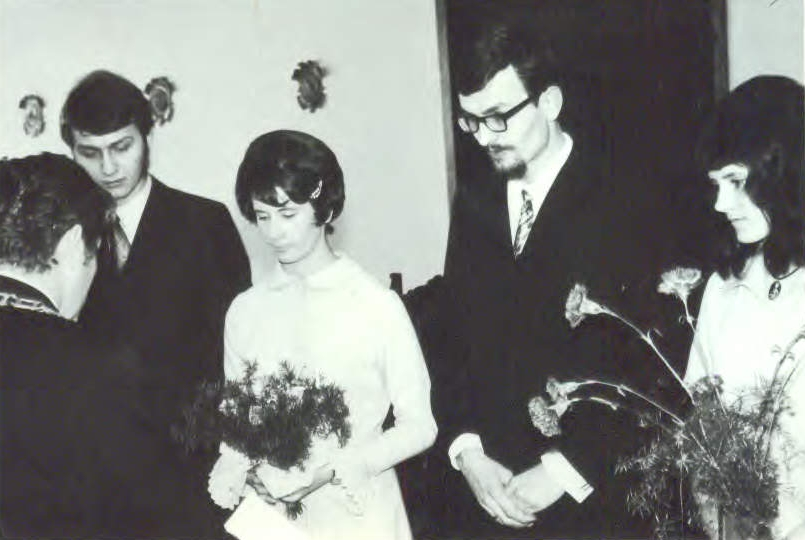
\includegraphics[width=0.5\textwidth]{photo/czeslawa_czeslaw_swierczynscy_slub_1.jpg}
\caption[Ślub Czesławy i Czesława Świerczyńskich]{Na zdjęciu od lewej: Tomasz Świerczyński, Czesława Głąbianka, Czesław Świerczyński, Mira Jabłońska}
\end{center}
\end{figure}

\textbf{Jeszcze na studiach pobraliśmy się 3 czerwca 1972 r. ze studentką tego samego roku studiów – Czesławą Głąb, ślub kościelny wzięliśmy 27 sierpnia tego roku w Kościele pw. św. ap. Piotra i Pawła w Katowicach.}
\begin{figure}[!h]
\begin{center}
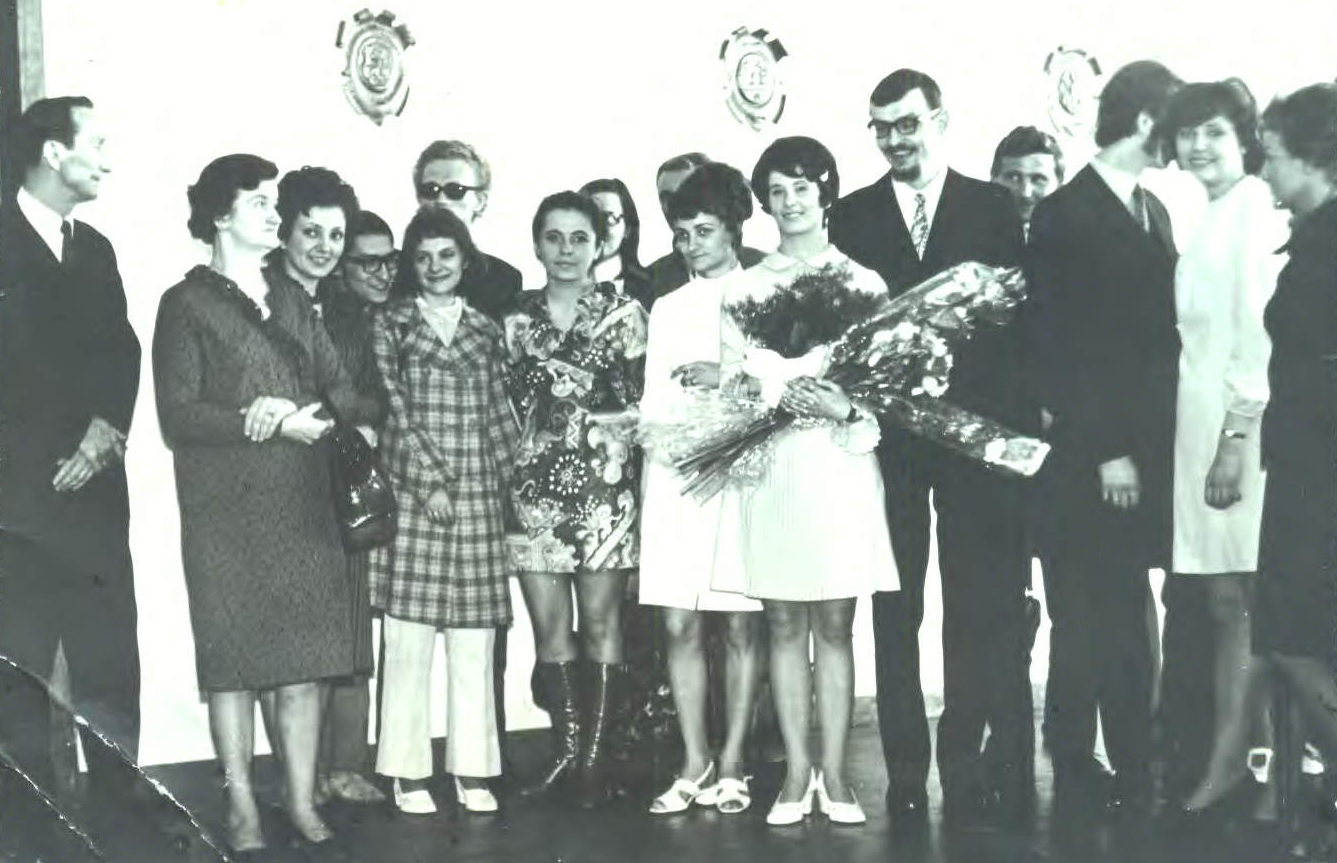
\includegraphics[width=\textwidth]{photo/czeslawa_czeslaw_swierczynscy_slub_2.jpg}
\caption[Ślub Czesławy i Czesława Świerczyńskich -- zdjęcie zbiorowe]{Na zdjęciu od lewej: Benedykt Świerczyński, Radegunda Świerczyńska, Barbara Tura, Y. Zaborowski, Majka Jędrecka, Mieczysław Dworaczek, Krystyna Oskwarek, Halina Błaszczyk, Czesława Głąb~-~Świerczyńska, Czesław Świerczyński, Eligiusz Błaszczyk, Tomasz Świerczyński, Urszula Skupin~-~Świerczyńska.}
\end{center}
\end{figure}

Wesele odbyło się wbrew tradycji w naszym domu, a nie w domu Panny Młodej w Mirowie, gdyż na kilka tygodni przed umówionym w Urzędzie Stanu Cywilnego w Katowicach terminem ślubu \textbf{zmarła 4 maja 1972 r. nieodżałowanej pamięci mama Czesławy – Eleonora Głąb}. Nasze małżeństwo z perspektywy lat owocne w znakomite potomstwo było i jest pełne cierni, których sobie wzajemnie nie żałujemy, bo to tak jakby Kochanowskiego ożenić z Rejem, który tak bardzo dbał o dobra materialne, że schodził z tego świata jako właściciel 40 miast i dwóch miasteczek, ale w obejściu był wulgarny i obsceniczny, czego się nie wstydził nawet w wierszach. Kochanowski natomiast majątku swego nie pomnożył, ale poezją swoją wprowadził język polski na szczyty kultury europejskiej, nigdy też nie był wulgarny, wolał opuścić dwór Zygmunta Augusta i porzucić karierę polityczną, niż pójść na jakiekolwiek układy z chamstwem choćby jaśniepańskim.

\textbf{Po studiach podjęliśmy we wrześniu 1973 r. pracę w Zespole Szkół Zawodowych Nr 1 w Myszkowie, ja w Technikum dla Dorosłych najpierw u dyr. Flankowskiego, a następnie u dyr. E. Wolaka, a pani Czesława u dyr. E. Samka w bibliotece.}

Przez pierwsze cztery lata mieszkaliśmy w Mirowie, w domu rodzinnym waszej Mamy, wraz z jej \textbf{Tatą a waszym dziadkiem – Franciszkiem, jej bratem Mirosławem, jego kolegą Alfredem Majewskim z Rodaków oraz tzw. dziadkiem – Stanisławem Kołaczem}, który służył u teścia za wikt i opierunek.
\begin{figure}[!h]
\begin{center}
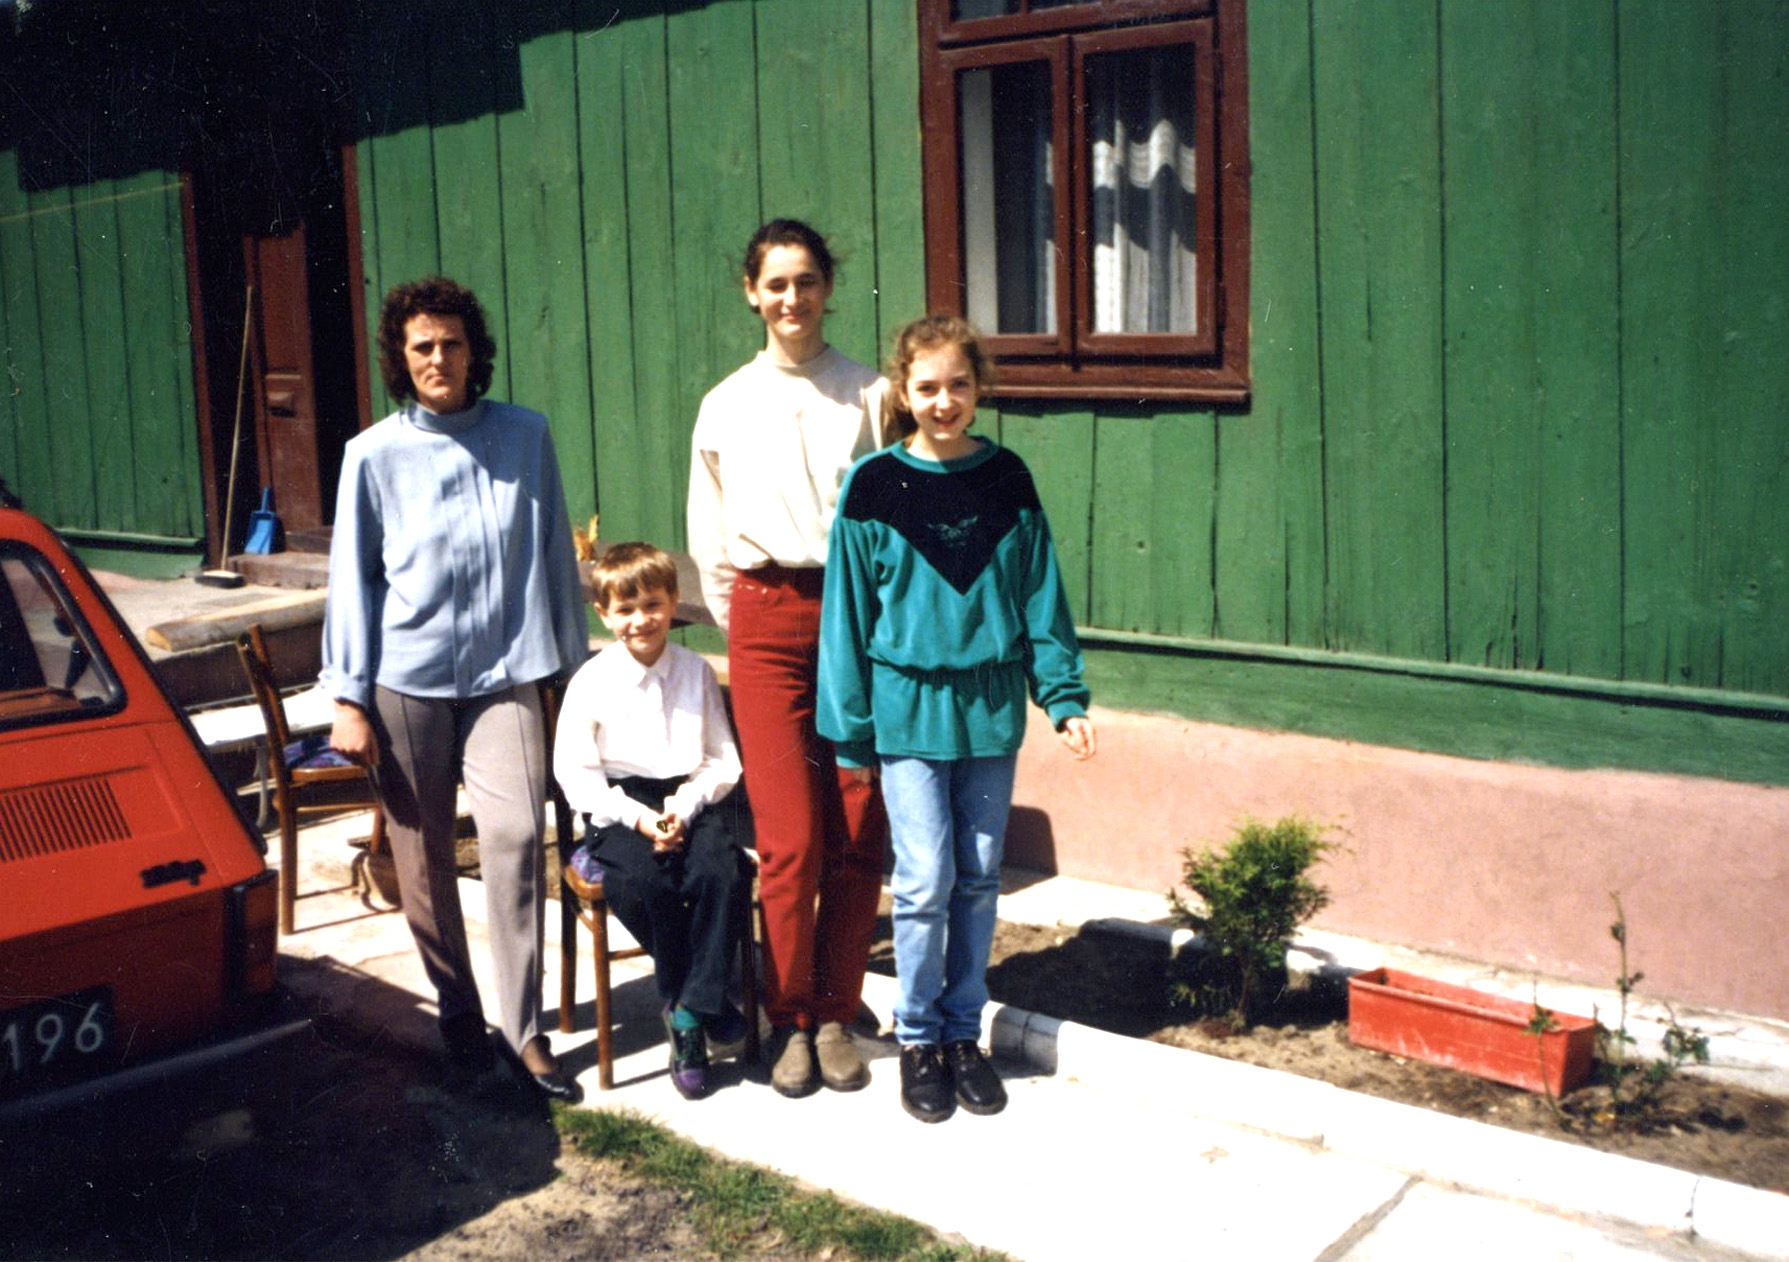
\includegraphics[width=0.6\textwidth]{photo/mirow_dom.jpg}
\caption[Nieistniejący już Dom w Mirowie z Elżbietą, Agnieszką i Krystianem Głąbami]{Na zdj. nieistniejący już Dom w Mirowie z Elżbietą, Agnieszką i Krystianem Głąbami}
\end{center}
\end{figure}

Bardzo serdeczny człowiek z nieodzownym papierosem w palcach, pełen wspomnień ze służby w wojsku carskim, często mówiący po rosyjsku, w ostatnich miesiącach życia zaczytywał się w „Pamiątkach Soplicy” Henryka Rzewuskiego, które wuj Mirosław włożył mu do trumny. Wszędzie z dziadkiem Franciszkiem Głąbem chodzili razem i siedzieli razem, a ze względu na ich zwyczaj Mirosław nazwał ich \textbf{Zukwą i Dźmuchą}, co znakomicie oddawało ich fizjonomię, jako że Dziadek Franek ciągle coś jadł nieustannie poruszając żuchwą, a „dziadek” Stanisław ciągle palił wypuszczając kłęby dymu. 

Ciasno było w tym domu, ale wesoło i miło. Tam też od pierwszych tygodni swego życia psociła \textbf{Zuzanna Eleonora}, nasze \textbf{pierwsze dziecko, pierwsza wnuczka} dziadków Świerczyńskich, \textbf{pierwsza prawnuczka	} Prababci Zofii Wilczek \textbf{oraz pierwsza i jedyna praprawnuczka praprababci Franciszki Jerominek}. Gdy skończył się urlop macierzyński i wychowawczy dla Czesławy, za zgodą dyrekcji uczyłem za siebie 24 godziny lekcyjne i za mamę Zuzi 22 godziny, co razem stanowiło 46 godzin tygodniowo, średnio po 8 godzin dziennie.

\textbf{W 1977 r. otrzymaliśmy mieszkanie w bloku przy ul. Strażackiej 35}, na trzecim piętrze w trzeciej klatce od Ośrodka Zdrowia. Stąd do pracy w Zespole Szkół Zawodowych mieliśmy bardzo blisko, z okien naszego mieszkania widać okna naszej szkoły, w której wszystkie lata pracy spędziła wasza Mama.
\begin{figure}[!h]
\begin{center}
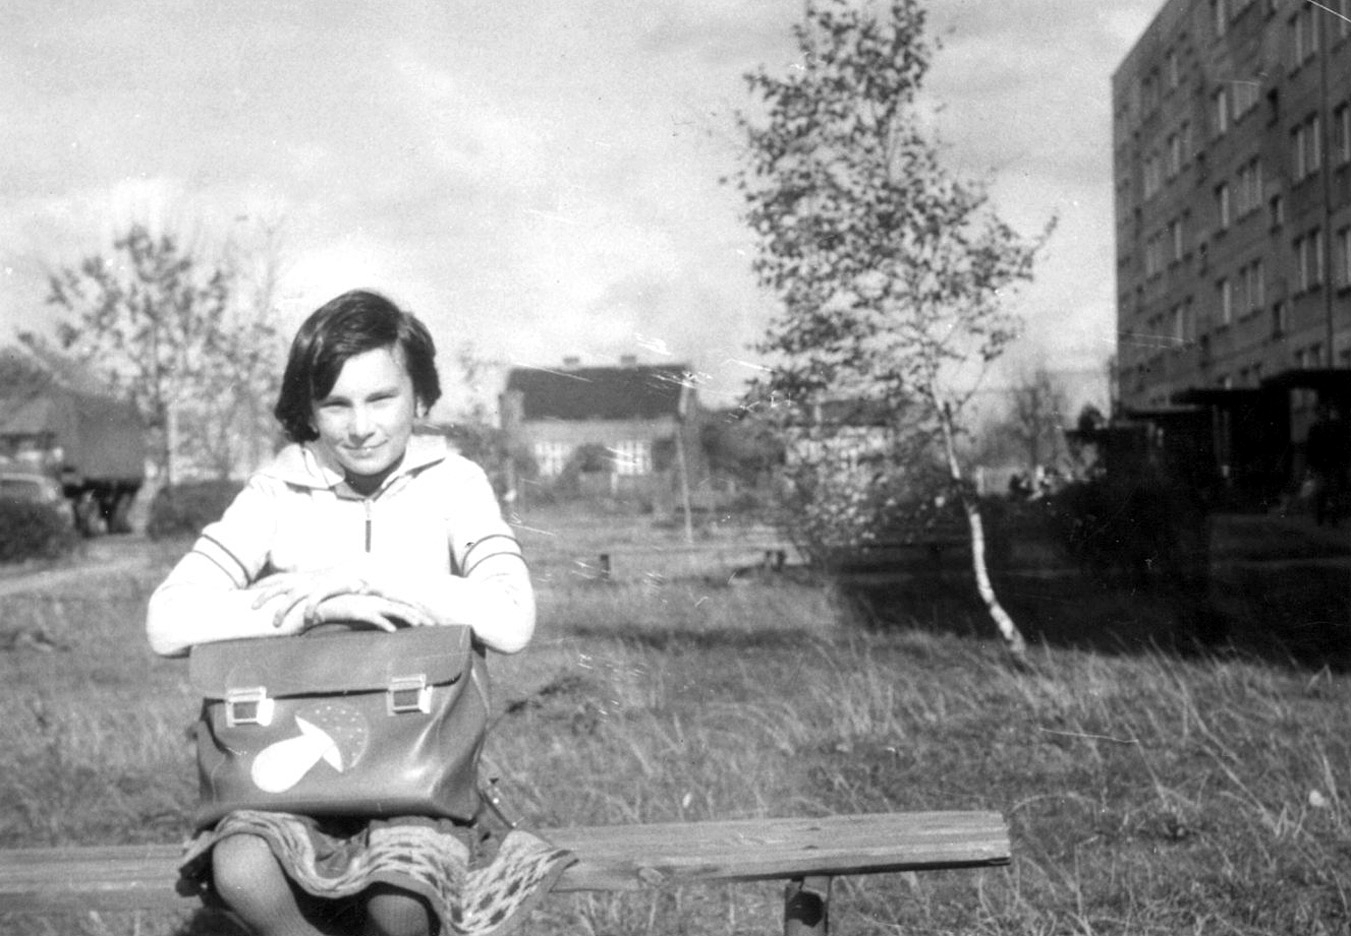
\includegraphics[width=0.6\textwidth]{photo/zuzia_swierczynska_1.jpg}
\caption[Zuzanna Świerczyńska na tle naszego bloku przy Strażackiej 35]{Na zdj. Zuzanna Świerczyńska siedzi na ławeczce na tle naszego bloku przy Strażackiej 35.}
\end{center}
\end{figure}

Wokół naszego bloku Myszkowska Spółdzielnia Mieszkaniowa posadziła brzozy,  wierzby, klony, modrzewie, dęby i jarzębiny, z których po latach wyrósł wcale okazały park. Do sąsiadów za to nie mieliśmy szczęścia. Drzwi w drzwi zamieszkał Zbigniew Cupiał – ubek działający w IV antykościelnym wydziale i alkoholik, ze swą żoną Janiną, również alkoholiczką. Zresztą w jego pionie zamieszkali (z wyjątkiem parteru) sami alkoholicy, którzy - z wyjątkiem Cupiała – wymarli (ich żony alkoholiczki żyją nadal). Nad nami mieszkali Noworolowie – muzycy, którzy wkrótce przenieśli się do Krakowa. Po nich przyszli Józef i Wanda Puczydłowscy, z którymi wasza mama była skłócona, a to z powodu wieszania mokrego, ociekającego wodą prania. Pani Wanda zmarła w 2002 r., a na miejsce pana Józefa wprowadził się jego syn z urodziwą synową. Pod nami mieszkali państwo Miklasowie, podobno spokrewnieni z Czesławem Miklasem – I sekretarzem Komitetu Powiatowego PZPR, wybitnie uciążliwa we współżyciu rodzina, zwłaszcza małżonka, będąca w konflikcie ze wszystkimi sąsiadami z wyjątkiem Płaczków. Pan Miklas uciekł się nawet do gróźb względem czteroletniego Piotrusia, za co został skazany przez Sąd Rejonowy w Myszkowie. \textbf{Najlepszymi naszymi sąsiadami byli państwo Błaszczykowie oraz państwo Ryszard i Ilona Angierowie.}

Pan Ryszard – były naczelny inżynier MFNE trzymał dyscyplinę i porządek w naszym bloku. Póki żył i był sprawny fizycznie był wokół bloku porządek i ład. Pani Błaszczykowa po śmierci męża kupiła dom przy ul. M. Reja, dokąd się wyprowadziła. Malowała obrazy, z czego po części się utrzymywała. Kilka z jej obrazów jest w naszym mieszkaniu (zwłaszcza ten duży z jadalni). W tym samym bloku mieszkali też na trzecim piętrze, ale w drugiej klatce od ul. Polnej państwo\textbf{ Jan i Krystyna Blecharczykowie} – nasi serdeczni przyjaciele – również nauczyciele Zespołu Szkół Zawodowych (przedmiotów zawodowych) – obecnie na emeryturze.

\begin{figure}[!h]
\begin{center}
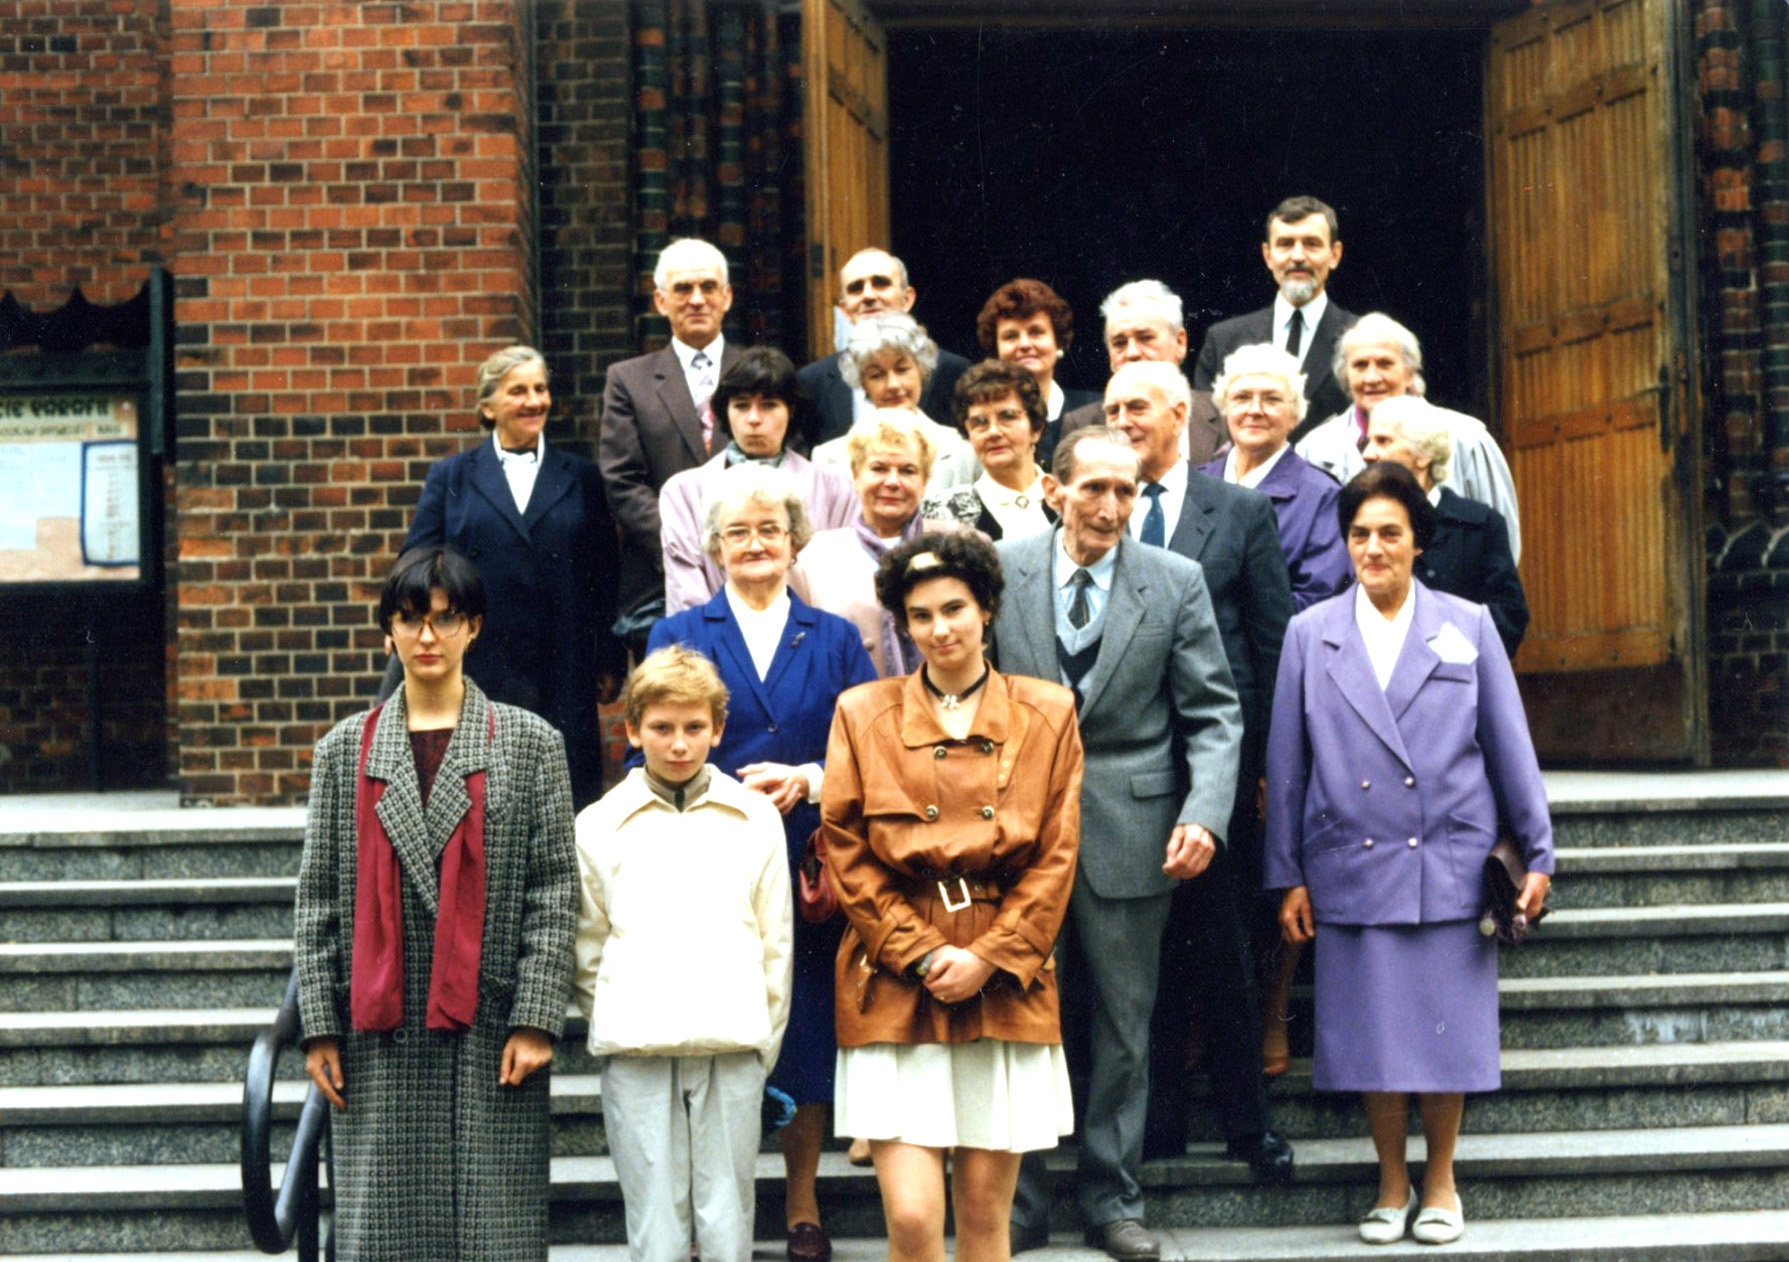
\includegraphics[width=0.8\textwidth]{photo/rodzina_swierczynskich_kosciol_piotra_pawla.jpg}
\caption[Złote Gody Radegundy i Benedykta Świerczyńskich -- zdjęcie zbiorowe]{Na zdj. przed kościołem Piotra i Pawła w Katowicach stoją od lewej: w I rzędzie Alina Świerczyńska, Bożydar i Zuzanna Świerczyńscy -- wnuczki i wnuk Złotych Jubilatów, w II rzędzie Jubilaci: Radegunda i Benedykt Świerczyńscy i Bronisława Witek, w III rzędzie Rita i Walery Wilczkowie, w IV rzędzie Joasia Wilczkówna (córka Antoniego), Ewa Wilczek (żona Antoniego), Maria Pluszczak, Barbara Prele, oraz Gertruda Kukowka (siostra prababci Zofii Wilczek), w V rzędzie Romuald Pluszczak i Irena Lehman, w VI rzędzie Maria Jerominek (siostra prababci Zofii Wilczek), Antoni Wilczek, Jan Wilczek z żoną Ireną i Czesław Świerczyński.}
\end{center}
\end{figure}

\textbf{18 września 1995 r. moi rodzice obchodzili Złote Gody}, czyli 50 rocznicę ślubu. Zjechała się cała jeszcze wówczas żyjąca rodzina Świerczyńskich i Wilczków.

\begin{figure}[!h]
\begin{center}
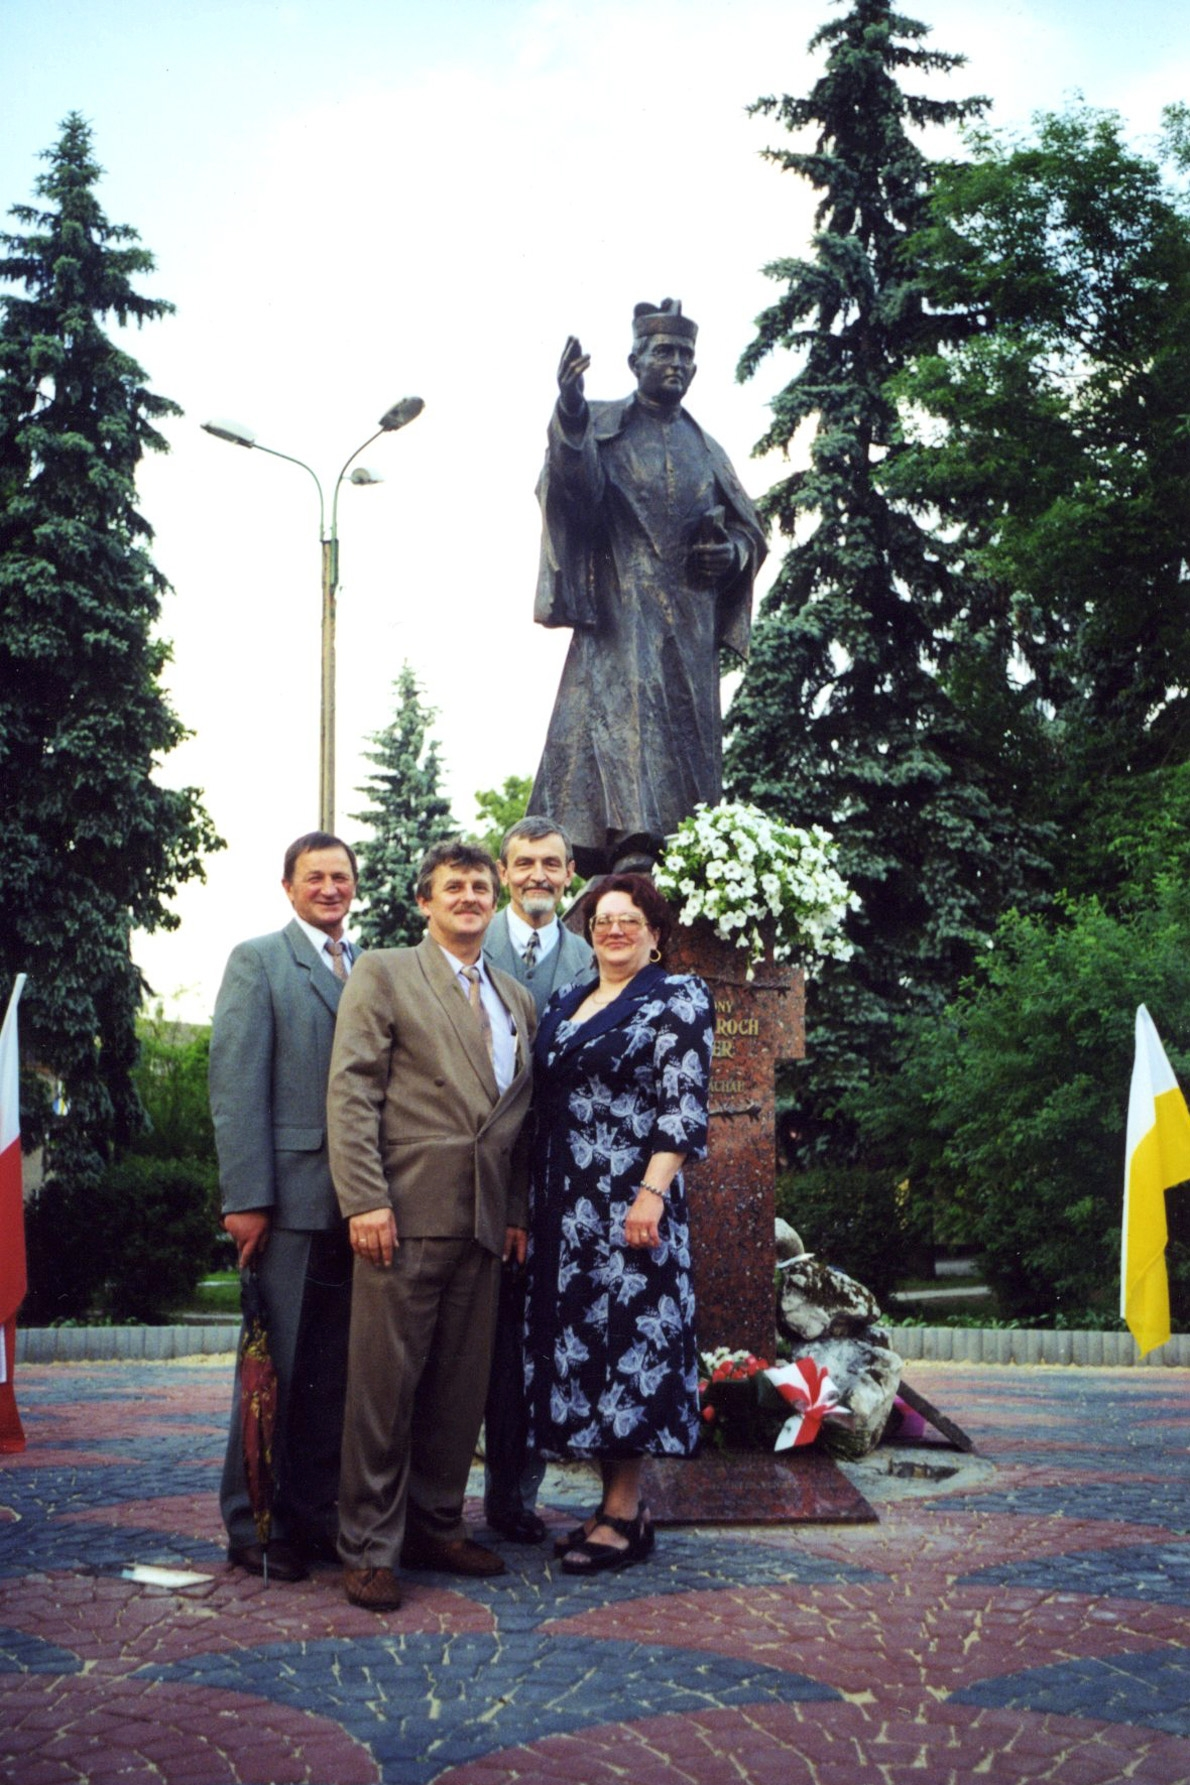
\includegraphics[width=0.5\textwidth]{photo/krystyna_jan_blecharczykowie.jpg}
\caption[Jan Blecharczyk, Włodek Gołuchowski, Czesław Świerczyński, X. Holi pod pomnikiem błog. ks. Rocha Gietyngiera w Żarkach]{Na zdj. Jan Blecharczyk, Włodek Gołuchowski, Czesław Świerczyński, X. Holi pod pomnikiem błog. ks. Rocha Gietyngiera w Żarkach.}
\end{center}
\end{figure}

\textbf{19 lipca 1999 r. zmarł mój Tato a wasz Dziadek Benedykt} w łóżku, w domu przy ul. Skłodowskiej 21 do końca w miarę sprawny. Jeszcze swoje 79 urodziny 23 lutego w niezłej kondycji przeżył. Pogrzeb odbył się 22 lipca, jakby dla podkreślenia jego ideowych związków z tym byłym świętem państwowym PRL-u.

W Roku 2000 -- Jubileuszowym -- wasz wujek -- \textbf{Mirosław Głąb przepisał nam zupełnie darmo działkę – część pola Pod Łysą Górą}, która dzięki moim staraniom, stała się działką budowlaną. 8 września – w Święto Narodzenia Najświętszej Marii Panny w Kancelarii Notarialnej Grażyny Buły wujek Mirek z nami i Rafałem Jabłońskim podpisał umowę darowizny i oświadczenie o ustanowieniu służebności drogi, na mocy której przekazał nam działki $295~m~/~1~m$ oraz $295~m~/~3~m$ o łącznej powierzchni 2119 $m^{2}$ a także Rafałowi Jabłońskiemu działkę $295~m~/~4~m$ o powierzchni 1309 $m^{2}$ przylegającą do naszej działki. 18 października owego roku geodeta uprawniony Jerzy Płatek dokonał wyznaczenia położenia na otrzymanej  działce wybranego przez nas typowego projektu budynku mieszkalnego typu „Leda”. 23 października potężna koparka w kilka dni wykonała wykop pod budynek z piwnicami.

28 października \textbf{Heniu Gryl} – nasz znakomity murarz wykonał zbrojenia ław fundamentowych, które już 4 listopada były z gruszki zalewane pod wodzą ś.p. Antoniego Surowca – wówczas pracownika firmy betoniarskiej Krzysztofa Polaka, dzięki czemu użyty doń beton był przedniej marki. 10 listopada ekipa murarska Henia Gryla ze swym pomocnikiem Wiesiem rozpoczęła stawianie murów piwnic. Ta ekipa odkryła, że ławy budynku zostały przez pomyłkę poszerzone o 1,8 m na szerokości budynku. Jeszcze w grudniu 2000 r. skończyli ich budowę i zalali schody wejściowe.

Wszystkie te działania, zwłaszcza ich organizacja mogły się dokonać jedynie dzięki niezwykłemu zaangażowaniu mojego szwagra, a waszego wujka Mirosława Głąba. Tam przecież było szczere pole, działka bez prądu i wody. Dopiero na wiosnę 2001 r. postawiono szopę – melaminę z blachy falistej, która do dzisiaj stoi przy ogrodzie. Sieć wodociągową doprowadzono w 2004 r. Do tego momentu wodę przywoził wozem konnym w cysternie wujek Mirek. W 2001 r. nasi dzielni murarze zalali strop nad piwnicami na początku maja, a już w pierwszych dniach czerwca skończyli mury parteru.

W końcu czerwca ekipa \textbf{Antka Surowca wraz z Henrykiem Grylem zalewają strop nad parterem}. A mury rosły dalej, aż do planowanej więźby dachowej. Przyjeżdża pod koniec lipca \textbf{ekipa Ryszarda Borczyka} „Tirem” wyładowanym drewnem konstrukcyjnym, które sięgało wyżej niż postawione mury. Boże, jak oni klęli, ale robota paliła im się w rękach. W połowie sierpnia, nasz znakomity dekarz – \textbf{Eugeniusz Starczewski} rozpoczął krycie dachu dachówką cementową, z czym się uwinął do końca tego miesiąca.

I wyobraźcie sobie, że w czasie wszystkich robót dachowych nie spadła jedna kropla deszczu, tak że Mirowianie sobie żartowali, że póki u Świerczyńskich robią z dachem, deszczu nie będzie. Tak Opatrzność czuwała nad naszą budową i czuwa nadal za przyczyną Matki Najświętszej... Istotnie, gdy Starczewski zszedł z dachu, następnego dnia spadł pierwszy od miesiąca deszcz. Wielki jest Pan i cudowna Jego Matka!

W 2001 r. \textbf{Bożydar} zdawał maturę i egzamin wstępny na studia techniczne. Lecz nim zaczął studiować we Wrocławiu zdążył jeszcze postawić płot betonowy \textbf{pod dyrekcją i z pomocą wujka Mirka}. W tym czasie byłem gościem na budowie, gdyż pełniłem funkcję wiceprezesa Myszkowskiej Spółdzielni Mieszkaniowej. W 2002 r. zostały wykonane tynki i wylewki w piwnicach oraz szambo i cała kanalizacja. To był trudny dla nas rok. Zuzia wyszła za mąż a mnie w dramatycznych okolicznościach pozbawiono pracy w MSM. \textbf{Zmarła też wówczas, tj. 25 X 2002 r. w szpitalu w Zabrzu moja Mama, a wasza Babcia – Radegunda}. W tym też czasie ukradziono nam okno dachowe poprzez wycięcie z więźby dachowej. W 2003 r. pan \textbf{Piotr Ludwikowski} wykonał jedynie instalację elektryczną w piwnicach oraz mur oporowy okalający schody wejściowe. Wtedy też Bożydar wraz z Piotrusiem w czasie swych wakacji wykonali z kostki brukowej chodnik prowadzący od furtki do schodów i wejścia pod schodami. Znakomita robota, co widać najlepiej z okna łazienki na poddaszu.

W tym też roku Piotruś wykonał skalniak na szambie wraz z ogrodzeniem, a Bożydar budę dla naszego psa Remika, który się oszczenił opodal naszego domu -  w lesie. Bożydar też wykonał wszystkie zabezpieczenia otworów okiennych i drzwiowych wraz z drzwiami balkonowymi od strony południowej.

W 2004 r. zdołaliśmy nareszcie doprowadzić wodociąg do naszego budynku. Nie trzeba już było wozić wody cysterną. W 2005 r. pan \textbf{Jarosław Kasznia} wykonał u nas instalację wodną w piwnicach, a w 2006 r. instalację wodociągową w całym budynku natomiast w 2007 r. instalację grzewczą w całym budynku.

\begin{figure}[!h]
\begin{center}
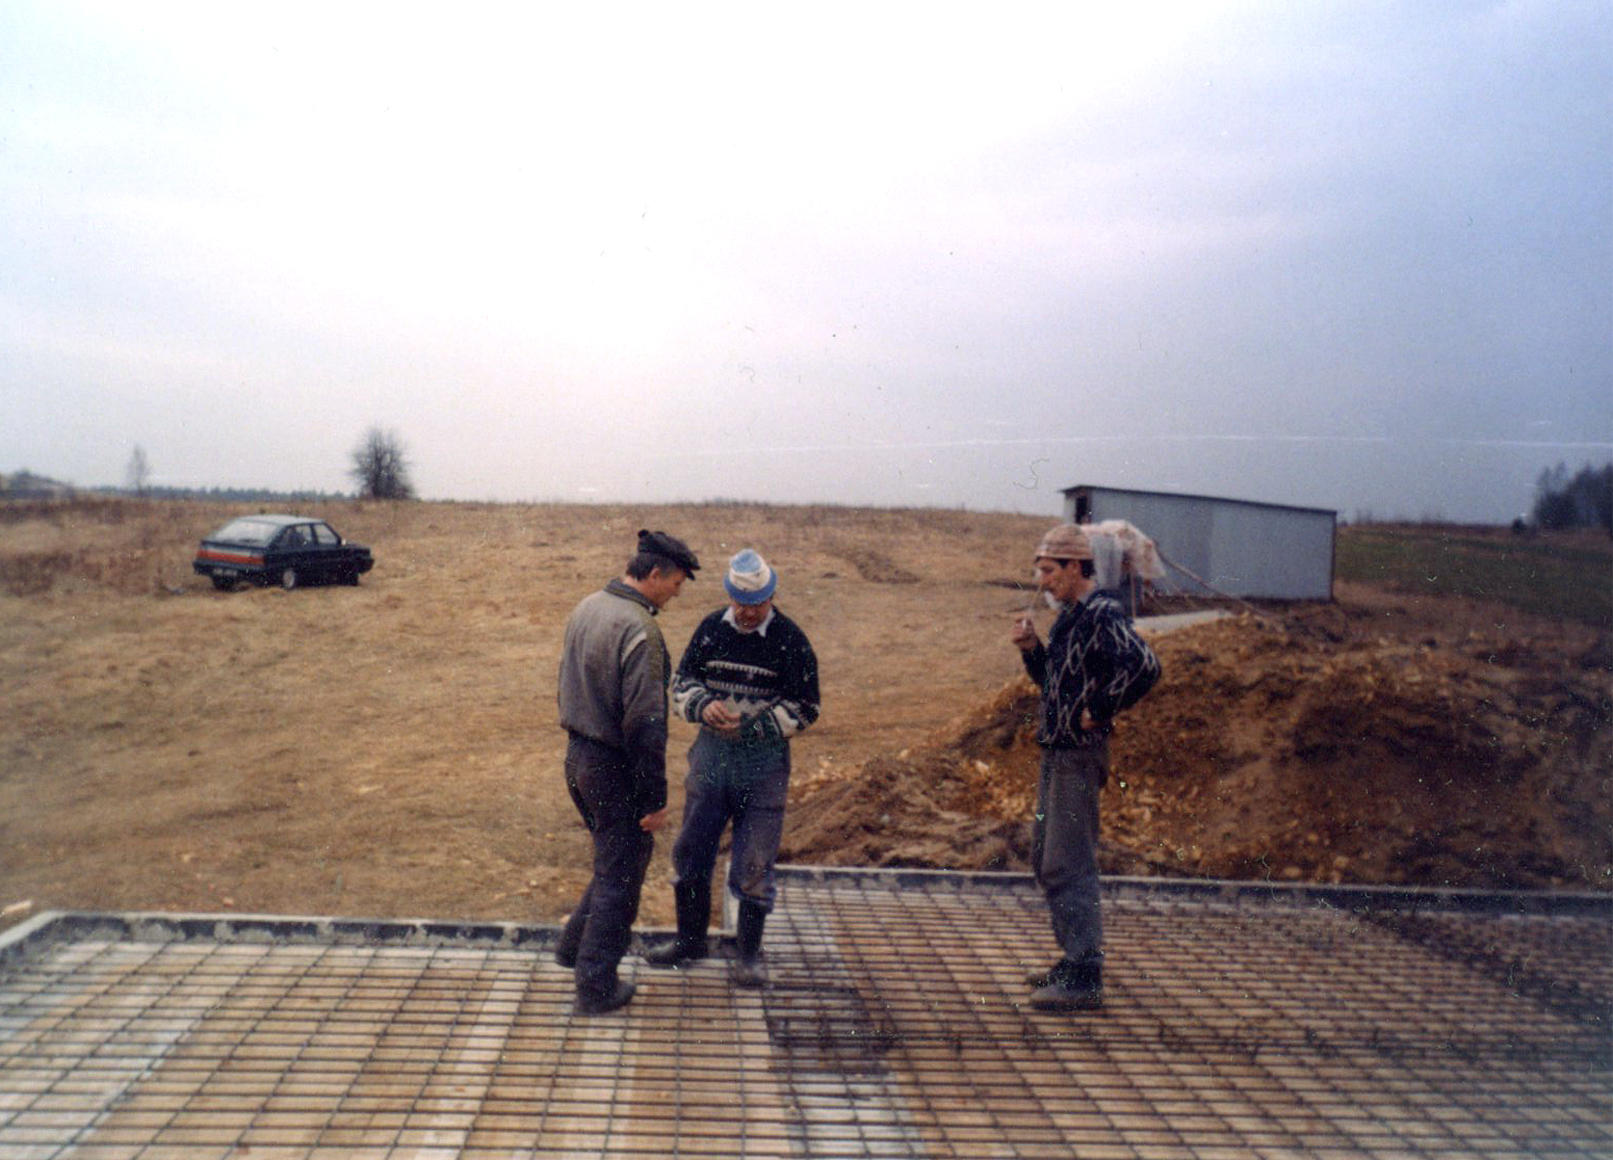
\includegraphics[width=0.65\textwidth]{photo/mirow_budowa_1_strop.jpg}
\caption[Mirów, budowa domu Świerczyńskich]{Budowa domu p. Świerczyńskich w Mirowie - przygotowanie pod wylewkę pierwszego stropu. Od lewej: Mirosław Głąb oraz murarz Henryk Gryl z pomocnikiem.}
\end{center}
\end{figure}

W 2005 r. pan \textbf{Janusz Podsiadło} wyłożył piwnice kafelkami (zwłaszcza łazienkę i kuchnię) a Bożydar ściany w przedpokoju, w kuchni i na schodach piwnicy wyłożył panelami – to kawał dobrej roboty. W 2006 r. \textbf{Paweł Balwierz} zamontował na parterze wszystkie okna i położył tynki na parterze i na poddaszu, (białkowanie wykonał piszący te słowa) zaś w 2007 r. wykonał wylewkę na obu piętrach i zamontował troje drzwi balkonowych na poddaszu. W 2008 r. ekipa \textbf{Krzysia Kordusa} (w składzie: Krzysiu Kordus – szef oraz Bożydar i Piotruś – pomocnicy) wykonali w weekend majowy gipserę salonu, jadalni, przedpokoju i pokoju północno-zachodniego. Piękna robota. W ciągu dwóch lat Bożydar korzystając z urlopu i sobotnich pobytów w Mirowie założył alarm i domofony (te ostatnie wymagają dokończenia). W grudniu nareszcie pan \textbf{Jan Skiba} z firmy „Piramida” z Zawiercia założył drzwi wewnętrzne na parterze, zaś pan \textbf{Eugeniusz Starczewski} założył w pokoju zachodnim na poddaszu okno dachowe oraz schody dachowe, a piszący te słowa rozpoczął ocieplanie dachu wełną mineralną.

\textbf{W 2008 r. nadano naszemu budynkowi numer 64, tj. $8^{2}$}, co dla mnie ma znaczenie symboliczne, bowiem liczba osiem oznacza NMP, tutaj do potęgi, czyli Jej potęgę, jej przemożną nad tym domem opiekę, \textbf{a ponadto zacząłem mój pobyt w Mirowie pod numerem ósmym, a pewnie skończę pod tym samym numerem, lecz do potęgi drugiej}. Ten numer został nadany bez żadnych z mojej strony sugestii. W tym też roku 9 września nasz dom został przez Powiatowego Inspektora Nadzoru Budowlanego uznany za odpowiedni do użytkowania w celach mieszkalnych.

W 2009 r. dokończono ocieplanie dachu  i położono płyty gipsowe sufitowe na całym poddaszu użytkowym pod kierownictwem pana \textbf{M. Semena}. \textbf{Janusz Podsiadło} położył kafelki w łazience, w kuchni, w dwóch przedpokojach i w salonie na parterze oraz na balkonach. Piszący te słowa  położył panele w pokoju południowo i północnozachodnim i odeskował cały strych (o powierzchni większej niż ma nasze mieszkanie w Myszkowie). W 2010 r. ekipa \textbf{Mirosława Dzieży z Łutowca} wykonała ocieplenie naszego budynku i położyła tynki w kolorze żółtym (góra) i ciemnozielonym (dół). Natomiast ekipa \textbf{Dariusza Sikorskiego} wykonała podbitkę pod dachem, zaś ekipa domowników pod czujnym okiem Krzysia Kordusa kładzie wokół budynku krawężniki, by pas między nimi a ścianami domu wypełnić białym grysem. Jeszcze w tym roku Piotruś położył bruk na tarasie oraz wykonał skosy pochyłe wypełnione grysem. W 2011 r. zabudowaliśmy wnękę w korytarzu szafą wnękową, a Piotruś wykonał schody brukowe na taras. Chcemy kupić i zamontować kocioł węglowy a także około 200 żeberek kaloryferów.

Mimo to czeka nas jeszcze ogrom wydatków i pracy. Trzeba kupić drzwi wewnętrzne na klatkę schodową oraz ośmioro drzwi na poddasze, trzeba w pokojach i w salonie na poddaszu położyć panele podłogowe oraz balustrady na balkonach i poręcze przy schodach i na klatce schodowej. Trzeba jeszcze wykończyć i wyposażyć sanitariaty na poddaszu oraz kuchnię na parterze. By można było w tym domu mieszkać w godziwych warunkach należy pozyskać sporą gotówkę... Jedynym wyjściem z tej trudnej sytuacji będzie zapewne sprzedaż mieszkania w Myszkowie...

Wróćmy jednak do moich dziejów, które obfitowały w wydarzenia zaskakujące, wynikające z inspiracji tzw. losu, czyli Opatrzności Bożej oraz mojej życiowej niezaradności, braku roztropności czy nawet głupoty, lecz zawsze były one powodowane szlachetnymi pobudkami. W 1976 r.  z trzech szkół ponadpodstawowych utworzono Zespół Szkół Zawodowych pod dyrekcją Tadeusza Tarłowskiego – pyszałka, głupca i złodzieja po trupach wspinającego się ku szczytom kariery. W związku z tym utworzono w naszej szkole odrębne Ognisko ZNP (Związku Nauczycielstwa Polskiego). Należało zatem wybrać nowy zarząd i jego prezesa. Nikt nie chciał zostać prezesem, bo to była funkcja społeczna przysparzająca dodatkowych kłopotów. Wobec tego władze szkoły sztucznie przedłużały posiedzenie Rady Pedagogicznej aż do wybrania pełnego składu Zarządu. Codziennie wtedy dojeżdżałem do Mirowa, więc czasu na takie dodatkowe imprezy nie miałem ochoty poświęcać. Mimo to zgłoszono moją kandydaturę na prezesa Zarządu Ogniska. Kolejne autobusy odjeżdżały nauczycielom, a ja nie chciałem się zgodzić na kandydowanie. W końcu koledzy nauczyciele podczas przerwy powiedzieli mi wprost: „Czesiek, nie bądź świnią, zgódź się.” I się zgodziłem po to, by być tylko figurantem, dla świętego spokoju, który wkrótce miał się skończyć wojną! Dyr. Tarłowski podsunął mi do podpisania zwolnienie kol. Wojtka Krykwińskiego z pracy w naszej szkole, bo to tylko formalność - mówił - gdyż on przenosi się do innej szkoły. Uwierzyłem i podpisałem.... Jakież było moje zdziwienie, gdy następnego dnia wieczorem do drzwi naszego mieszkania w Myszkowie zadzwonił tenże Wojtek, który powitał mnie słowami: Ty hu... Wyjaśniliśmy sobie wszystko...

Następnego dnia we władzach ZNP wycofałem swoją zgodę, ale na tym nie koniec. W kilka dni przeczytałem niemal wszystkie akty prawne dotyczące nauczycieli i ich uprawnień. Mało tego, zwołałem zebranie naszego Ogniska ZNP, na którym dyr. Tarłowskiego nazwałem oszustem oraz wymieniłem kilkanaście faktów łamania przez niego obowiązującego prawa nauczycielskiego. Szum był na cały powiat. Dałem mu czas miesiąca na naprawienie wymienionych nieprawidłowości, pod groźbą powiadomienia o nich Kuratora Oświaty i Wychowania w Częstochowie. Ten dureń jednak poszedł na konfrontację! Wysłaliśmy zatem pismo do Kuratorium w Częstochowie podpisane przez cały Zarząd ZNP wzbogacone o opis aktów malwersacji autorstwa dyr. T. Tarłowskiego.

Wezwano mnie jako prezesa ZNP do Kuratorium, gdzie czekała mnie cała zgraja różnych notabli z I sekretarzem KP PZPR, Kuratorem Oświaty i Wychowania oraz dyr. T. Tarłowskim, którzy przez ponad godzinę wrzeszczeli nade mną, a ja spokojnie wyłuszczałem im niezbicie, że ten oto siedzący pośród nich dyr. T. Tarłowski nie powinien dalej pełnić swojej funkcji, ponieważ dopuścił się licznych aktów łamania obowiązującego prawa, więc jeśli tylko władze oświatowe odwołają go z pełnionej funkcji, nauczyciele ZSZ będą gorliwie wypełniali swe nauczycielskie obowiązki. Po tym moim wystąpieniu powstała wrzawa nie do opisania, ale gdy zobaczyli, że niczego nie wskórają, podziękowali mi za przybycie i pożegnali się ze mną wszyscy przez podanie ręki z wyjątkiem Tarłowskiego...

Potem były nasze pisma do Ministerstwa Oświaty i Wychowania, do Zarządu Głównego ZNP (Związku Nauczycielstwa Polskiego), a nawet do Komitetu Centralnego PZPR. Natomiast nasi adwersarze wyżywali się na naszych małżonkach (na Czesławie i Krystynie Blecharczyk) oraz na wszystkich tych koleżankach, które nas popierały. Próbowano nas też wyeliminować z gry poprzez podważenie praworządności naszego wyboru do władz związku. Dyrektor Wolak na ogólnym zebraniu wszystkich członków Ogniska ZNP zapytał zebranych: „Jak to się stało, że Jan Blecharczyk wszedł do Zarządu Ogniska?”, a przecież to on właśnie kilka miesięcy wcześniej usilnie nakłaniał Jasia, by zechciał wejść do Zarządu! Dopiero Krysia Surma – żona ówczesnego wicedyrektora Liceum - przemówiła do sumień zebranych, przypomniawszy wszystkim okoliczności tamtego zebrania. Trzeba być moralną szmatą, by tak zakłamywać fakty, zdarzenia! Pojechaliśmy w końcu po wsparcie do Zarządu Głównego ZNP, do Warszawy, a tam się okazało, że większość tych wysoko postawionych związkowców, to dyrektorzy szkół! Był to zatem związek pracodawców a nie związek zawodowy pracowników oświaty. Tam też koledzy związkowcy zamiast nam przyjść z pomocą, zrugali nas i zapewnili, że pierwsi wystąpią przeciw nam – wichrzycielom!

Ponieważ opisaliśmy całą naszą sprawę także w liście skierowanym do KC PZPR, więc zostaliśmy wezwani przed oblicze samego I sekretarza KW PZPR – Grygla, ja z koleżankami: Zosią Okraską i Czesią Brych. Przyjął nas bardzo szczerze, po partyjnemu, zwracając się do nas słowami: „Wy huje! Jak dalej będziecie pisać, to wam, kurwa, kości połamiemy!” Ponieważ zwrócił się ów I sekretarz KW PZPR tymi słowy do moich koleżanek, co nijak do nich nie pasowało, choćby ze względu na ich płeć, więc roześmiałem się od ucha do ucha, a on wpadł w furię. Ryczał jak zwierzę, a wszyscy zebrani tam towarzysze mieli łby pospuszczane. Gdy przestał ryczeć, zwróciłem mu grzecznie uwagę, że Konstytucja PRL gwarantuje nam prawo pisania skarg do władz zwierzchnich, na co ten ryknął: „Ja wam kurwa dam konstytucję!” Na tym skończyła się nasza wizyta w KW PZPR w Częstochowie.

W konsekwencji urządzono wbrew prawu, bo przed upływem kadencji ponowne wybory do Zarządu Ogniska, które pod presją wszystkich czynników władzy przegraliśmy. Natomiast dyr. Tarłowski musiał opuścić naszą szkołę. Poszedł kraść do Technikum Rolniczego w Będuszu. Mnie zaś nowy dyrektor Młynarski powiedział, że nie mam co szukać w jego szkole. W kilka lat później, w 1983 r. to samo powtórzył Jasiowi Blecharczykowi, który zatrudnił się, podobnie jak ja, ale cztery lata później, w Hucie „Katowice”.

W Hucie „Katowice” zatrudniłem się na stanowisku kierownika Zakładowego Centrum Kulturalno Oświatowego dzięki protekcji sekretarza KW PZPR – Rudolfa Juzka – przyjaciela mojego Ojca jeszcze z lat wojny. Od sierpnia 1979 r. do sierpnia 1980 r. niewiele zrobiłem, parę imprez i remont pomieszczeń. Poznał się na mnie główny specjalista ds. kadr, który proponował mi inne stanowisko, lepiej płatne, ale niesamodzielne.

W 1979 r. przybył do Polski nasz rodak – Ojciec Święty – Jan Paweł II. Byłem wśród entuzjastycznie Go witających Polaków na Jasnej Górze (dwa razy) oraz w Krakowie. Częstochowa jako miasto wystrojem swoim nie zachwyciła, natomiast Kraków przeszedł wszelkie wyobrażenia człowieka wychowanego w „komunie”! Flagi papieskie były wszędzie, nawet na kilkunastopiętrowych blokach, nawet na budynkach instytucji państwowych. W Krakowie po raz pierwszy poczułem się naprawdę wolny. A na Błoniach Krakowskich było nas grubo ponad trzy miliony. Morze ludzi. Bogu Wielkiemu niech będą dzięki, że mnie wyprowadził miłosierną dłonią z głupoty ateizmu przed wyniesieniem Karola Wojtyły do godności papieskiej. Kto wie, czy przez głupią przekorę nie byłbym trwał w swoim ateizmie i bez entuzjazmu odnotowywał kolejne wizyty papieskie w ojczyźnie...

W sierpniu 1980 r. wyjechaliśmy z Zuzikiem na rodzinne wczasy zakładowe do Łeby. Chcąc jej pokazać Gdańsk, katedrę w Oliwie zawędrowałem również pod bramę Stoczni Gdańskiej. Chcąc otrzymać jakiś ich biuletyn, zostawiłem Zuzika na ławce opodal i kazałem cierpliwie czekać, bo pod bramą był straszliwy ścisk. Ale wkrótce, nim cokolwiek zdobyłem odwołała mnie jakaś pani do zapłakanej Zuzi. Takie było jej pierwsze spotkanie z wielką polityką. Materiały jednak zdobyłem następnego dnia, ale wtedy byłem już bez mojego Szczęścia.

Po powrocie z wczasów od razu zaangażowałem się w działalność powstającego w Hucie „Katowice” Niezależnego Samorządnego Związku Zawodowego „Solidarność”, a zwłaszcza w pisanie artykułów do „Wolnego Zwiążkowca” redagowanego przez Zbyszka Kupisiewicza.

Szefem Międzyzakładowego Komitetu Strajkowego przy Hucie „Katowice” został Andrzej Rozpłochowski. Po wyjściu z internowania wyjechał do USA,  do niedawna mieszkający w Sacramento, obecnie chyba w Dąbrowie Górniczej. Do prezydium MKS-u został dokooptowany Kazimierz Świtoń – członek Ruchu Obrony Praw Człowieka i Obywatela oraz założyciel pierwszych w Polsce Wolnych Związków Zawodowych. Lecz niestety, zamiast pomocy od niego, prezydium MKZ-etu doczekało się z jego strony działań dywersyjnych i intryg do tego stopnia, że wysłano mnie w listopadzie do Gdańska, bym porozmawiał z Wałęsą, Kuroniem, Walentynowicz, Gwiazdą, Borusewiczem o postępowaniu K. Świtonia w naszych strukturach związkowych. 

Najpierw przyjął mnie w MKZ w Gdańsku Andrzej Gwiazda. Nie znał on jednak Świtonia, więc polecił mi się spotkać z Jackiem Kuroniem, który korzystał z gościny w domu Anny Walentynowicz. Wszedłem do kuchni, a tam nieprzeliczona gromada butelek po wódce, pośród której można się było poruszać jak bocian w sitowiu. Pan Jacek zadawał mi mnóstwo pytań nie dając żadnych rad, a przy tym nieustannie palił. W końcu spostrzegł się, że już zaczął się Dziennik telewizyjny, więc z zapalonym papierosem ruszył do salonu wyłożonego parkietem, gdzie stał telewizor. W trakcie oglądania dziennika dopalił mu się papieros, a że nie było w pobliżu popielniczki, bez żenady zgasił go na parkiecie przydeptując butem niedopałek. Gdy po latach opowiedziałem to senatorowi i zarazem profesorowi WSP w Kielcach - Stanisławowi Żakowi, ten odparł, że Kuroń to samo czyni z niedopałkami w salach sejmowych na marmurowej posadzce.

Noclegu użyczył mi Bogdan Borusewicz, który niewiele nam doradził, ale wyposażył  mnie w dość bogatą literaturę z drugiego obiegu i sporo nagadaliśmy się na wspólnie nas interesujące tematy z historiii literatury. Rano byłem umówiony z Lechem Wałęsą. Przyjął mnie znacznie później, wskazał mi miejsce i sam wcześniej usiadłszy  nogi położył na stole!... Włos mi się zjeżył na głowie, przez chwilę zmagałem się z myślą, by uczynić to samo, ale nie chciałem ryzykować fiaskiem mojej misji, więc usiadłem i pokrótce starałem się przedstawić nasz „świtoniowy” problem, lecz pan Wałęsa przerwał mi, by wygłosić tyradę o wszystkich swych wielkich dziełach, oraz że zrobiłby jeszcze więcej gdyby mu nie przeszkadzali. Najczęstszym słowem w tej przemowie był zaimek „ja”. Wyszedłem stamtąd przygnębiony, zdałem sobie bowiem sprawę, że człowiek tak pyszny a przy tym prostak może nas niestety wyprowadzić na manowce...

Zimą przybył na Śląsk – do „Spodka” Lech Wałęsa i zajął miejsce w prezydium z Kazimierzem Świtoniem i naszym Andrzejem Rozpłochowskim. To był ostatni triumf Kazia Świtonia... Jego nieustanne intrygi, rozpuszczanie plotek mających skompromitować Andrzeja i to, jak się okazało, powielanych na naszym sprzęcie, doprowadziły wreszcie do tego, że Andrzej zdecydował się na przeprowadzenie głosowania wśród delegatów, dzięki któremu miało się okazać ilu delegatów popiera Rozpłochowskiego a ilu Świtonia. \textbf{Liczyliśmy na wygraną Andrzeja, ale niewielką różnicą głosów. Wyniki głosowania okazały się dla nas wielkim radosnym zaskoczeniem: na ponad 500 delegatów tylko kilkunastu głosowało za Świtoniem!} Decyzją Delegatów K. Świtoń został usunięty z prezydium MKZ. A wydawało się, że tak wielu delegatów go popiera, że wręcz stanowi zagrożenie dla Andrzeja. \textbf{Z tego głosowania wyciągnęła daleko idące wnioski ubecja, która poprzez swoich TW zrobiła wszystko, by Andrzej Rozpłochowski na zjeździe zjednoczeniowym nie został wybrany na przewodniczącego Zarządu Regionu Śląsko – Dąbrowskiego NSZZ „Solidarność”.}

Jeszcze przed listopadem napisałem artykuł pt. „Jak zniszczyć naród”, którego po raz pierwszy nie puściła cenzura, co zostało zaznaczone pod wymienionym tytułem w nawiasie kwadratowym, że cały artykuł nie został dopuszczony do druku przez cenzurę.

Kiedy jednak udało mi się wydrukować ów artykuł w gazecie „Soldarności” Kaliskiej, wówczas i „Wolny Związkowiec” i „Solidarność” Mazowsza też ten artykuł opublikowały. A było w nim napisane, że jakieś ciemne siły w Polsce realizują szatański plan zniszczenia polskiego narodu! Ten plan jest do dzisiaj, lecz ze znacznie większym impetem realizowany, jednak wydaje się, iż ostrzeżenia płynące obecnie zwłaszcza z rozgłośni Radia „Maryja” przez wielu Polaków, jeśli nie przez większość, są ignorowane. Za ten artykuł oraz za artykuły ukazujące mechanizmy zniewalania narodu poprzez tzw. „haki” jakie sprawujący władzę wówczas z Moskwy, a dziś także z Berlina, Tel Awiwu i Manhatanu... usiłowali i usiłują zniszczyć nasz naród, a następnie opanować zajmowany przez niego obszar między Odrą a Bugiem, \textbf{za te artykuły zostałem zakwalifikowany do elitarnej grupy internowanych...}

19 marca 1981 r. doszło do tzw. „prowokacji bydgoskiej” kiedy to milicja pobiła w sali sesyjnej Wojewódzkiej Rady Narodowej w Bydgoszczy działaczy „Solidarności” z Janem Rulewskim na czele. Z tego powodu miał się odbyć strajk generalny okupacyjny. W związku z tym zarząd MKZ Huty „Katowice” miał się przenieść na czas strajku generalnego do Huty „Baildon”. Tak się też stało. Spaliśmy na przysłowiowym styropianie. Jakież było nasze rozgoryczenie i gniew, gdy po kilku dniach takich przygotowań, by cały naród był gotów do walki o należne mu prawa – dowiedzieliśmy się z Dziennika Telewizyjnego, że Lech Wałęsa bez konsultacji z Prezydium Związku podjął decyzję o odwołaniu strajku generalnego. To był pierwszy wyraźny sygnał potwierdzający słowa Anny Walentynowicz, że Wałęsa jest kapusiem i zdrajcą, nie tylko prostakiem i kabotynem. Wróciliśmy do swoich zajęć, gdyż 7 kwietnia miał się ukazać pierwszy numer „Wiadomości Katowickich”, dziennika NSZZ „Solidarność” ukazującego się do 11 grudnia włącznie. Redaktorem naczelnym był pan Andrzej Czuma, obecnie min. Sprawiedliwości z poręki Platformy Obywatelskiej...\textbf{Ileż zacnych ludzi w tych latach, przez swoje błędy dało się przez ubecję zeszmacić!}

Potem był zamach na Ojca Świętego Jana Pawła II i moja z sześcioletnią Zuzią gorąca modlitwa o Jego życie! Przecież jeszcze przedszkolaczek, a potrafił się ze swym tatą modlić cały różaniec o życie Jana Pawła II. Pod koniec miesiąca zmarł Prymas Tysiąclecia – Interrex – kardynał Stefan Wyszyński. Koledzy jechali na ów wielki pogrzeb, a ja sobie wymyśliłem, że zdążę być i na pielgrzymce mężczyzn w Piekarach Śląskich i na pogrzebie Prymasa Wyszyńkiego. Co za głupota! Szatan mnie jeszcze nie raz tak „wyrolował” podsuwając przysłowiowemu osiołkowi i owies i siano. Dobrze, że przy mnie rodzina nie doznała głodu. Lecz to już zasługa miłosiernego Boga! Uczestniczyłem w tych wielkich uroczystościach jak większość Polaków za pośrednictwem telewizji, a mogłem być w Warszawie...

W maju lub w czerwcu odbyła się pielgrzymka ludzi pracy do sanktuarium franciszkańskiego Matki Bożej z Lourdes w Katowicach Panewnikach. Całe to wydarzenie z udziałem Biskupa Herberta Bednorza, prowincjała franciszkanów - Damiana Szojdy oraz całego prezydium MKZ Huty Katowice zostało przeze mnie zorganizowane, co mi zasugerowali: o. Oskar Puszkiewicz, Joasia Jarzębińska oraz Kaziu Trojan. W ramach tej pielgrzymki ogłosiliśmy zamiar budowy pomnika dzieci nienarodzonych, które zginęły z woli swoich rodziców, a pod presją gomułkowskiej ustawy aborcyjnej z 1958 r. Podczas tej uroczystości po raz pierwszy na Śląsku pojawiły się w dużej liczbie flagi z charakterystycznym napisem „Solidarność” sugerującym demonstrujący tłum pod polską flagą.

Produkcję tych flag było mi dane zorganizować, za co później ubecja poprzez swoich konfidentów w „Solidarności” próbowała mnie zniszczyć, sugerując że produkcja była nielegalna, nieopodatkowana, ale ja miałem i mam do dzisiaj dokumenty poświadczające uczciwość moich działań. Te działania wspierał  nasz szef – Andrzej Rozpłochowski, też tylko mający wówczas wykształcenie zasadnicze w zawodzie mechanika samochodowego, ale był to człowiek zawsze skromny i nie kabel, jak Wałęsa... Niestety, potem przyszedł sierpień i zjazd zjednoczeniowy, na którym wycięto Andrzeja, a jego miejsce zajął Tadeusz Jedynak, człowiek antykościelny, nie wykazujący jakiegokolwiek zrozumienia dla ratowania życia nienarodzonych. Wróciłem do pracy w Hucie „Katowice” na stanowisko jakiegoś referenta, gdyż po rzuceniu legitymacją partyjną nie mogłem już być kierownikiem ZCKO.

13 grudnia o godzinie 24 z soboty na niedzielę zapukali do nas smutni panowie, którzy przedstawili się jako milicja. Ja im odpowiedziałem, żeby sobie przyszli o 6 rano w poniedziałek, gdyż to jest właściwa pora na załatwianie spraw służbowych. Oni na to, że wyłamią drzwi. Poprosiłem ich o chwilę czasu by się przyodziać. Ucieczka nie miała sensu z III piętra w grudniu, więc postanowiliśmy z mamą wpuścić ich, tym bardziej że mama była z Bożysiem przy nadziei, a sześcioletnia Zuzia spała w średnim pokoju. Panowie pozwolili mi się spokojnie ubrać, nawet mogłem się chwilę pomodlić, dziękując Panu Bogu, że pozwolił mi złożyć za ojczyznę ofiarę z wolności i polecając Mu całą moją rodzinę.

% TODO *** Tu zdjęcie naszego ołtarzyka w mieszkaniu myszkowskim

Mama Była przekonana, że tylko na kilka godzin mnie zabierają, ja natomiast byłem pewien, że na co najmniej kilka miesięcy jeśli nie lat, oraz że tymi aresztowaniami objęty jest cały kraj, bo przecież ja byłem w „Solidarności” Śląskiej pionkiem, więc jeśli mnie zamykają, to na pewno wszystkich ode mnie ważniejszych... Zawieźli mnie reprezentacyjną czarną „Wołgą”  do Komendy Wojewódzkiej MO (Milicji Obywatelskiej) w Częstochowie. Stało tam sporo takich jak ja internowanych, ale mnie zupełnie nieznanych, gdyż ja działałem na terenie wojew. katowickiego (a oni działali w ówczesnym woj. częstochowskim). Po wylegitymowaniu zapakowali nas do „suk”, czyli więźniarek i wieźli w nieznanym kierunku. Wszyscy tam palili, że aż sino było od dymu, a mnie się zbierało na wymioty. Zawieźli nas nad ranem do więzienia w Zabrzu Zaborzu. Mnie wraz z Józefem Lamchem z Tomiszowic – działaczem „Solidarności Rolników Indywidualnych” wpakowali do celi z jedną piętrową pryczą bez materacy i bielizny pościelowej, ale z otwartym oknem, od którego oddzielały nas kraty oddalone od tego okna o jakiś metr. Nie można go było zamknąć, a na dworze mróz poniżej -10~\textcelsius. Mnie głowę chciało rozsadzić po tej dwugodzinnej podróży w zadymionym samochodzie, a pana Józefa bolało serce, bo był po dwóch zawałach i tym bardziej doskwierał mu chłód, gdyż zabrali go z domu w niekompletnym stroju, w kalesonach i bez butów, jako że bronił się zaciekle przed aresztowaniem. Dzielny, szlachetny człowiek i niezłomny działacz „Solidarności RI”, a przede wszystkim wielki patriota.

Dopiero wieczorem w niedzielę przenieśli nas do wieloosobowej celi, w której spotkałem sporo kolegów z „Solidarności” hucianej, a także Kazia Trojana. Oni mnie znali i mogli kolegów z Częstochowy przekonać, że nie jestem jakąś „wtyką”. W składzie osobowym tej celi znalazło się kilku znakomitych opowiadaczy dowcipów, że boki można było zrywać do późnej nocy. Był też tam z nami górnik o imieniu Waldemar, który niedawno, bo w „Barbórkę” dostał order „Sztandar Pracy” II klasy, jedno z najwyższych odznaczeń PRL-u. My wszyscy i on sam byliśmy przekonani, że internowali go przez pomyłkę. Przesiedział z nami kilka dni opowiedziawszy sporo śląskich dowcipów, a przed wyjściem z więzienia zwrócił się do nas ze słowami: Panowie, jo dziynkuja Bogu, żech się tu dostoł, bo teroz wiym, że to cygaństwo, co godali, że Solidarność miała strzylać do partyjnioków”...
Jednak nie wszyscy byli tak optymistycznie nastawieni do otaczającej ich rzeczywistości... Zwłaszcza ci, którzy chcieli zrobić w „Solidarności” karierę snuli się smętnie po korytarzu więziennym, a z ich twarzy można było wyczytać słowa piosenki Kabaretu Starszych Panów: 
\begin{center}
\textit{„A tośmy, tośmy wpadli, 
A niech to wszyscy diabli...” }
\end{center}
By jednak duch we współwięźniach nie upadał zawiesiliśmy krzyż (wykonany z desek więziennej pryczy) na kracie zamykającej nasz korytarz. Kazali nam go zdjąć, ale nikt z nas ani spośród strażników więziennych nie odważył się tego zrobić. A co najważniejsze, każdego wieczoru, około godziny 22, gdy ludzie wracali z drugiej zmiany lub szli na nockę, zbieraliśmy się na apel wieczorny, który rozpoczynaliśmy pacierzem, a potem śpiewaliśmy przez dobre pół godziny pieśni kościelne i patriotyczne, zwłaszcza te, które władza ludowa zabraniała śpiewać. Na ten czas otwieraliśmy wszystkie okna, by całe Zabrze nas słyszało. Wyobraźcie sobie, jaka to była siła – ponad sto męskich głosów!... Nie muszę was przekonywać, że w ten śpiew bardzo się angażowałem. Po kilku dniach naszego gromkiego śpiewania o stałej porze słyszeliśmy, że pod murem więzienia gromadzą się ludzie. 

Na kilka dni przed Wigilią Bożego Narodzenia zamknęli też z nami księdza Stanisława Gębkę, (obecnie prałata i proboszcza bazyliki katedralnej w Częstochowie) pochodzącego z Będusza, co przyjęliśmy z wielką radością, spodziewając się, że w zbliżające się Święta - najbardziej polskie będziemy mogli uczestniczyć we Mszy św. Ksiądz Stanisław też miał taką nadzieję i dlatego wystąpił do władz więzienia o umożliwienie mu odprawienia  Mszy św. Jednak na dwa dni przed Wigilią ubecja zwolniła go z internowania...

Utworzyliśmy w tym więzieniu swego rodzaju władzę samorządową, której zadaniem było zredagowanie statutu internowanego i jego praw. Po kilku dniach i statut i prawa internowanego znalazły się na biurku kierownictwa więzienia w Zabrzu Zaborzu. Żądaliśmy też od władz więzienia, by dały nam na piśmie prawne uzasadnienie faktu przetrzymywania nas w areszcie więziennym przez ponad dwie doby. I ku mojemu zdumieniu dali nam takie uzasadnienia zapewne wyjęte z teczek ubeków. Mnie napisali m.in. że jestem nacjonalistą polskim! Czyż mógłbym kiedykolwiek otrzymać wspanialszą pochwałę mojego patriotyzmu. Kaziowi Trojanowi, który angażował się w Ruchu Obrony Życia napisali, że jest fanatykiem religijnym. Jednemu z przewodniczących Komisji Zakładowej NSZZ „Solidarność” napisali, że cieszy się sympatią i uznaniem załogi! Niestety, następnego dnia odebrano nam te uzasadnienia, a przecież wystarczyło tylko powiedzieć, że je wyrzuciłem...

W dzień przed Wigilią kazali nam się spakować, tzn. wszystko, co nasze zgarnąć do prześcieradła i uczynić z niego swoisty worek, w gwarze więziennej zwany mandżurem. Grudniowym wieczorem, bo już było ciemno, kazali nam wyjść przed barak więzienny, a tam czekał już na nas szereg suk. Między pierwszą suką a schodami wejściowymi do baraku stało kilkunastu strażników albo milicjantów – nie wiem, było ciemno – z pałkami w rękach, którzy drwiąco do nas szczerzyli zęby, więc nikt się nie kwapił iść pierwszy, a ci jakby z radością uderzali tymi pałkami o wewnętrzną stronę swej lewej dłoni. Pomyślałem sobie, że to wstyd okazać przed nimi strach, więc wciągnąłem wysoko, aż na głowę swój mandżur i ruszyłem pierwszy do suki... Nikt mnie nie uderzył. Za mną poszła reszta. 

Późnym wieczorem byliśmy już w więzieniu w Raciborzu. To było prawdziwe Alcatraz... Mury więzienia były ponad metrowej grubości, tak że ja chcąc zobaczyć przez luksferę  jakie jest niebo podciągałem się do samych krat więziennego okienka, a kolana miałem jeszcze na krawędzi muru. Okienko było okratowane prętami grubości ok. 3 cm. Siedzieliśmy w celach czteroosobowych z „kiblem” w środku. Między piętrami była zawieszona siatka na klatce schodowej. Codziennie mieliśmy pół godziny spaceru na spacerniku, bo o wyjściu na korytarz nie było co marzyć. Śniadania, obiady i kolacje mieliśmy wydawane o ściśle określonej porze z taką punktualnością, że można było według nich regulować zegarki. Toteż gdy pod koniec stycznia spóźniono się ze śniadaniem o kwadrans, byliśmy przekonani, że coś niezwykłego wydarzy się tego dnia...

I rzeczywiście, przewieziono nas wtedy do więzienia w Jastrzębiu – Szerokiej. W celi, w której przyszło mi spędzić kilka tygodni byli osadzeni oprócz mnie: dr Politechniki Gliwickiej – Grabowski zajmujący piętro pryczy nad Ciepielą. Ja zajmowałem również piętro pryczy nad byłym wychowankiem domu dziecka ( nie pamiętam jego imienia ani nazwiska). Nasi koledzy z dolnych pryczy, absolwenci szkół zasadniczych namiętnie grali w „Chińczyka”. Gdy im się już pod wieczór gra we dwójkę znudziła, wręcz nas błagali, byśmy z nimi zagrali. Właściwie nasza rola ograniczała się tylko do rzucania kostką do gry, gdyż oni poprzez wielogodzinne granie doszli do takiej wprawy w liczeniu, sumowaniu punktów i stawianiu bierek na właściwym miejscu, iż nasze mało wprawne działania w tym zakresie irytowały ich na tyle, że nas w tym zastępowali...

Więzienie w Jastrzębiu Szerokiej wspominam jako najgorsze, ze względu na panujące tam zimno i wilgoć. W naszej celi „zamieszkałej” tylko przez czterech internowanych – po uwolnieniu Jurka Hilbrychta pojawiły się przy oknie sople, gdyż pęknięty kaloryfer nie grzał, a nasza czwórka nie była w stanie wystarczająco jej zagrzać ciepłem własnych ciał. Więc gdy po miesiącu, na przełomie lutego i marca dokooptowano do nas czterech górników z „Wujka”, jeszcze tego wieczoru owe sople znikły. Spaliśmy w tych warunkach we wszystkim, co można było na siebie ubrać, a w ciągu dnia siedzieliśmy w wymiennikowni ciepła...W tych okropnych warunkach był przetrzymywany również Jerzy Krzempek, działacz „Solidarności” cierpiący na postępujący gościec i dlatego mógł się poruszać jedynie o kulach. Lekarze kilkakrotnie interweniowali u władz więziennych, by nie przetrzymywali Jurka Krzempka w takich warunkach. Sprzyjają one bowiem rozwojowi choroby, tak że może on utracić nawet władzę nad układem wydalniczym. Na to ubecy za każdym razem proponowali mu współpracę za cenę uwolnienia!

Moją celę dzieliłem z czterema kolegami: wspomnianym wyżej Jurkiem Hilbrychtem, Włodkiem Forysiem i Bargiełem z „Solidarności” Bielsko-Bialskiej oraz Gabrielem (zapomniałem nazwiska) z Politechniki Gliwickiej. Jurek Hilbrycht był lekarzem i o jego uwolnienie strasznie zabiegała jego żona. Był ponadto utalentowanym rysownikiem i na potrzeby naszej więziennej kaplicy zorganizowanej w innej pustej, więc nieogrzewanej celi, narysował czternaście stacji drogi krzyżowej, symbolicznie ukazujące ich istotę. Tam też po raz pierwszy podjęliśmy rozważania na temat encykliki Jana Pawła II „Laborem exercens” oraz poszczególnymi księgami Pisma Świętego, które kontynuowaliśmy do ostatnich dni naszego internowania. Włodek Foryś był przesympatycznym doktorem ekonomii świetnie grającym na gitarze, z którym dane mi było dzielić losy  internowanych aż do Łupkowa włącznie (wyszedł pewnie w listopadzie na wolność i wyjechał do Kanady ze swą dopiero co zaślubioną małżonką. Nasze więzienie w Jastrzębiu – Szerokiej odwiedzili dwaj wybitni hierarchowie: bp Herbert Bednorz – ordynariusz katowicki oraz kard. Franciszek Macharski – metropolita krakowski. W czasie wizyty bpa Bednorza Kaziowi Trojanowi udało się nakłonić go, by zezwolił wnieść na teren więzienia zakonsekrowane Hostie święte. W sobotę na widzeniu były już w naszej więziennej „Kaplicy”, w której podjęliśmy czuwanie przed Najświętszym Sakramentem, aż do radiowej Mszy św. w  niedzielę. Jakaż była nasza radość, gdy w czas komunii po raz pierwszy od 13 grudnia mogliśmy przyjąć Ciało Chrystusa. Zostaliśmy za to ukarani przez władze więzienne, co przyjęliśmy z wielką dumą. Dopiero w Jastrzębiu – Szerokiej miałem pierwsze widzenie z żoną Czesławą i córką – moim ukochanym Zuzikiem – to był jej drugi przykry kontakt z wielką polityką. Mimo że wasza Mama była w zaawansowanej ciąży z Bożysiem, to Myszkowska Komenda Milicji Obywatelskiej uznała za stosowne zwodzić ją co do miejsca mojego aktualnego pobytu, w związku z czym Mama odwiedziła najpierw więzienia w Zabrzu – Zaborzu i w Raciborzu! Takie milicyjne chamstwo...

23 marca w południe zapakowali nas do „suk” i powieźli w nieznanym kierunku. Koledzy z krakowskiego poznali przez sufitowy wywietrznik, że wiozą nas przez Kraków dalej na wschód... Czyżby zatem miała się realizować owa optymistyczna wersja losów opozycji antykomunistycznej, że pojedziemy na Syberię (wersja pesymistyczna zakładała, że tam dotrzemy piechotą)? Późnym wieczorem zajechaliśmy do więzienia w Tarnowie, gdzie nas uraczyli herbatą i powieźli dalej na wschód. Gdy udręczeni wielogodzinną podróżą nareszcie opuszczaliśmy suki z mandżurami, powitały nas gromkie śpiewy naszych kolegów z „Solidarności” rzeszowskiej. To była jeszcze Polska – Uherce Mineralne w Bieszczadach! Nareszcie w miarę ciepło w celach i możliwość całodziennego pobytu na spacerniku. Tam poznałem mojego serdecznego przyjaciela – Waldka Mikołowicza z Jarosławia i wielu, wielu innych z całego południa Polski.
\begin{figure}[!h]
\begin{center}
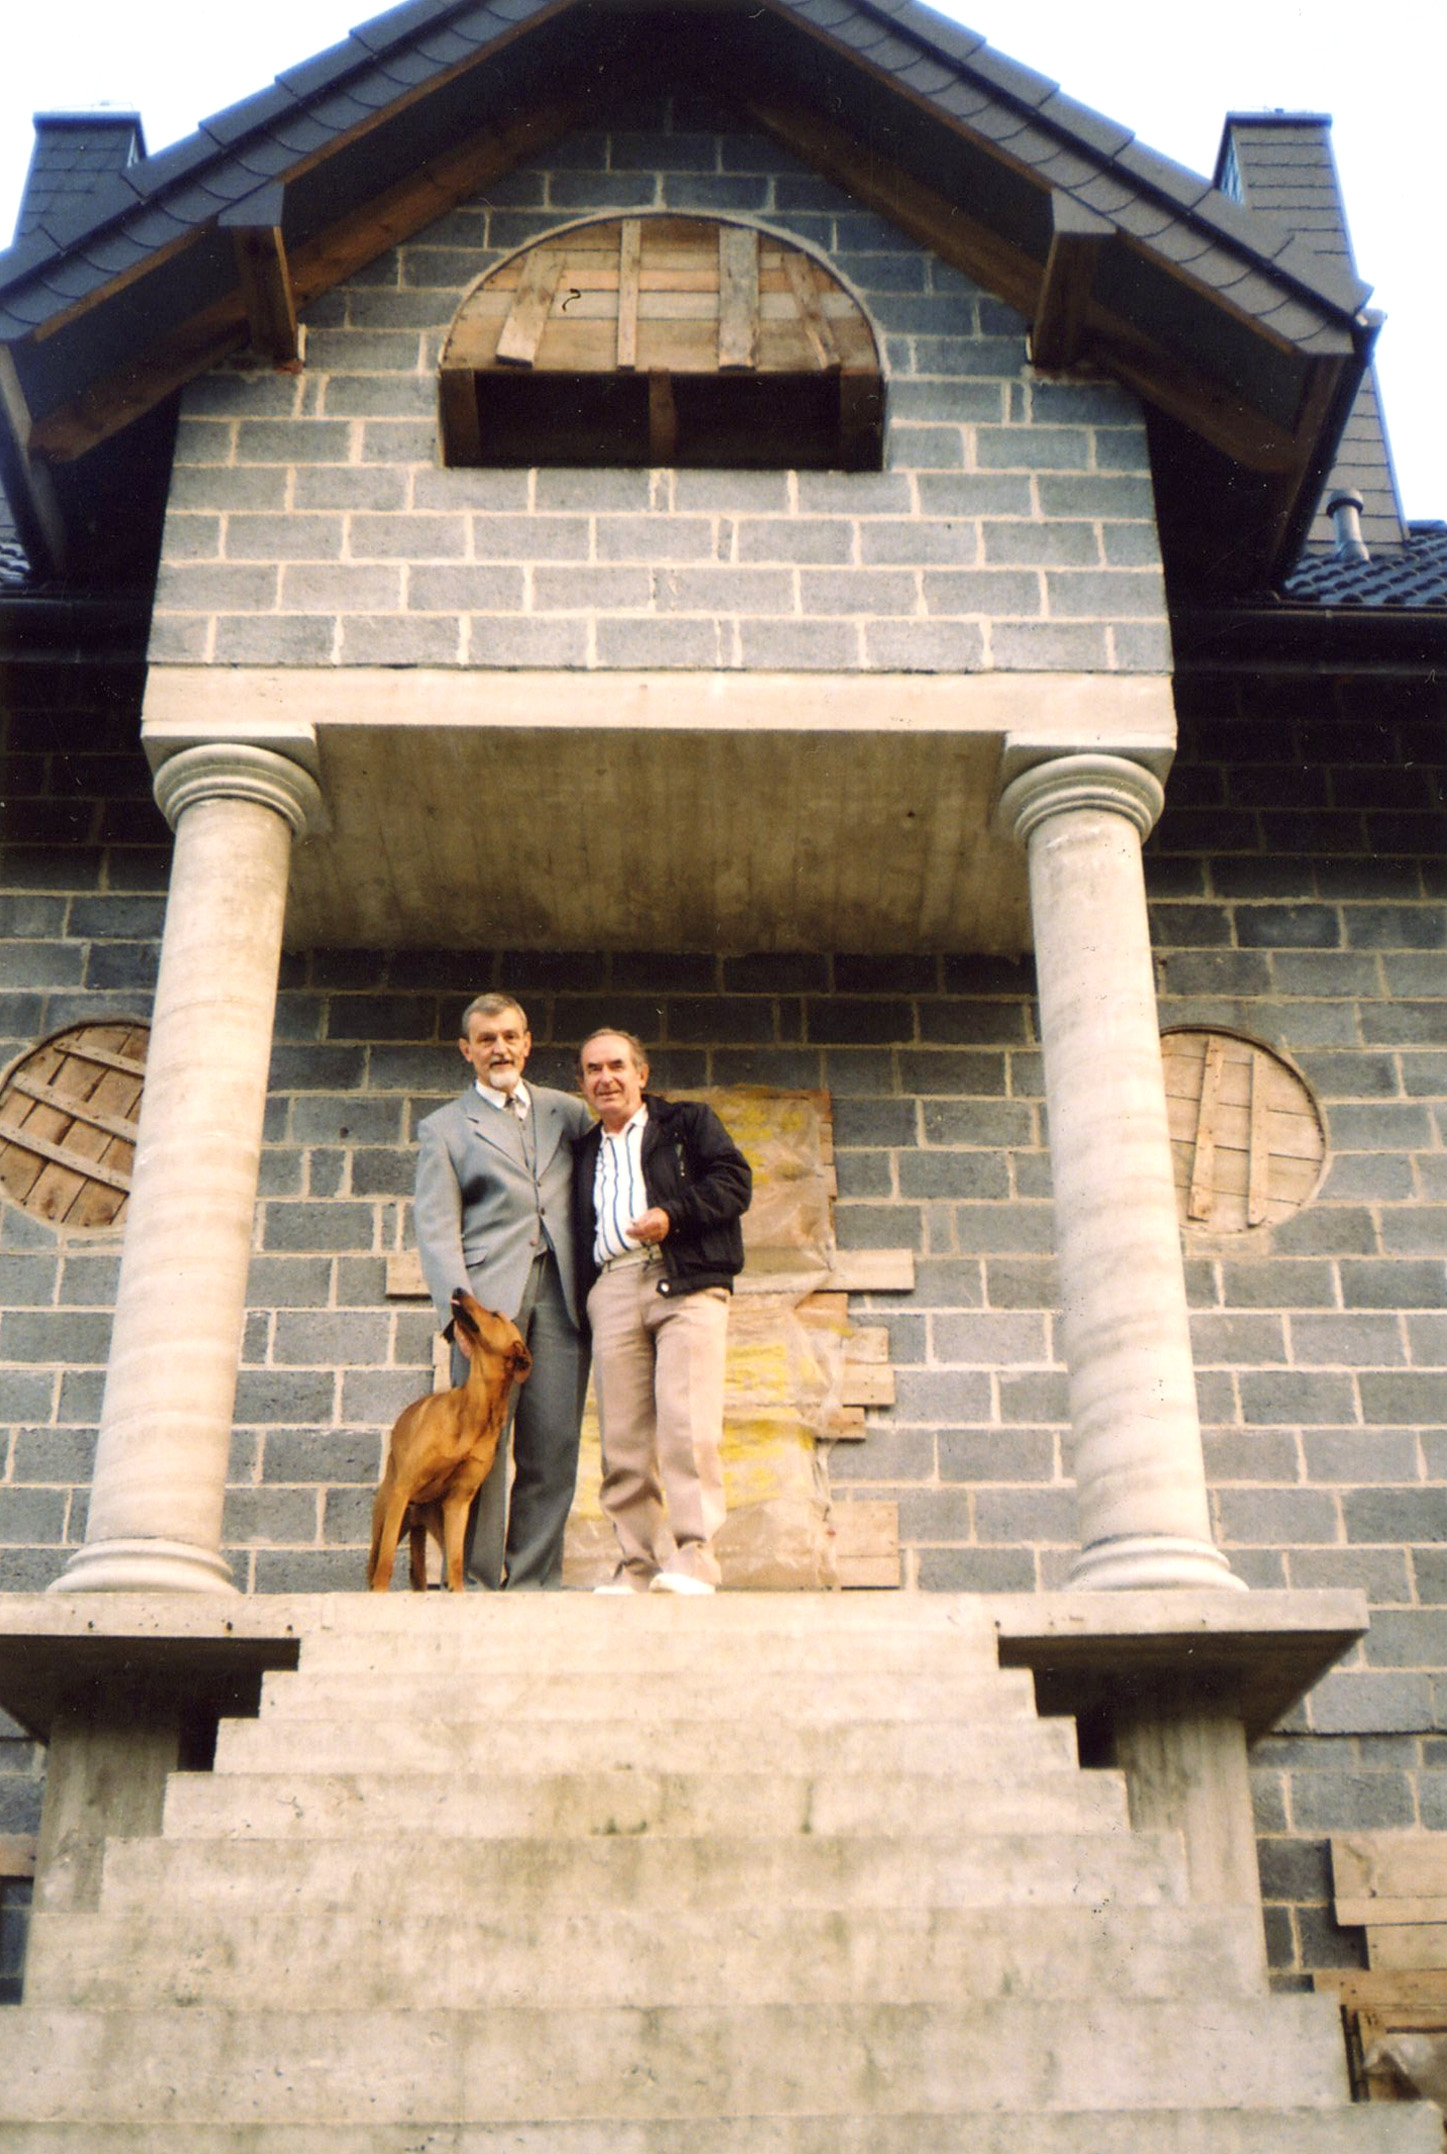
\includegraphics[width=0.45\textwidth]{photo/waldemar_mikolowicz_1.jpg}
\caption[Waldemar Mikołowicz z Czesławem Świerczyńskim w Mirowie]{Na zdj.Waldemar Mikołowicz z autorem tych wspomnień w naszym domu w  Mirowie}
\end{center}
\end{figure}

Tam też nareszcie mieliśmy Mszę św. w niedziele i święta. Oczywiście urządziliśmy w jednej z cel stałą kaplicę. W Wielki Piątek dane mi było poprowadzić całą „drogę krzyżową” pod stacjami narysowanymi przez Jurka Hilbrychta. Tam też od kolegów z Podkarpacia nauczyłem się śpiewać „Gorzkie żale”. A potem była Wielkanocna Resurekcja w więziennych murach, na której zebrało się co najwyżej dwie trzecie internowanych. Wkrótce też nastały nabożeństwa „Majowe”, które dane mi było prowadzić. To był piękny czas... Wolno było posiadać instrumenty muzyczne, więc koledzy przygrywali do melodii litanijnej. Podobnie było też podczas nabożeństw czerwcowych...
\begin{figure}[!h]
\begin{center}
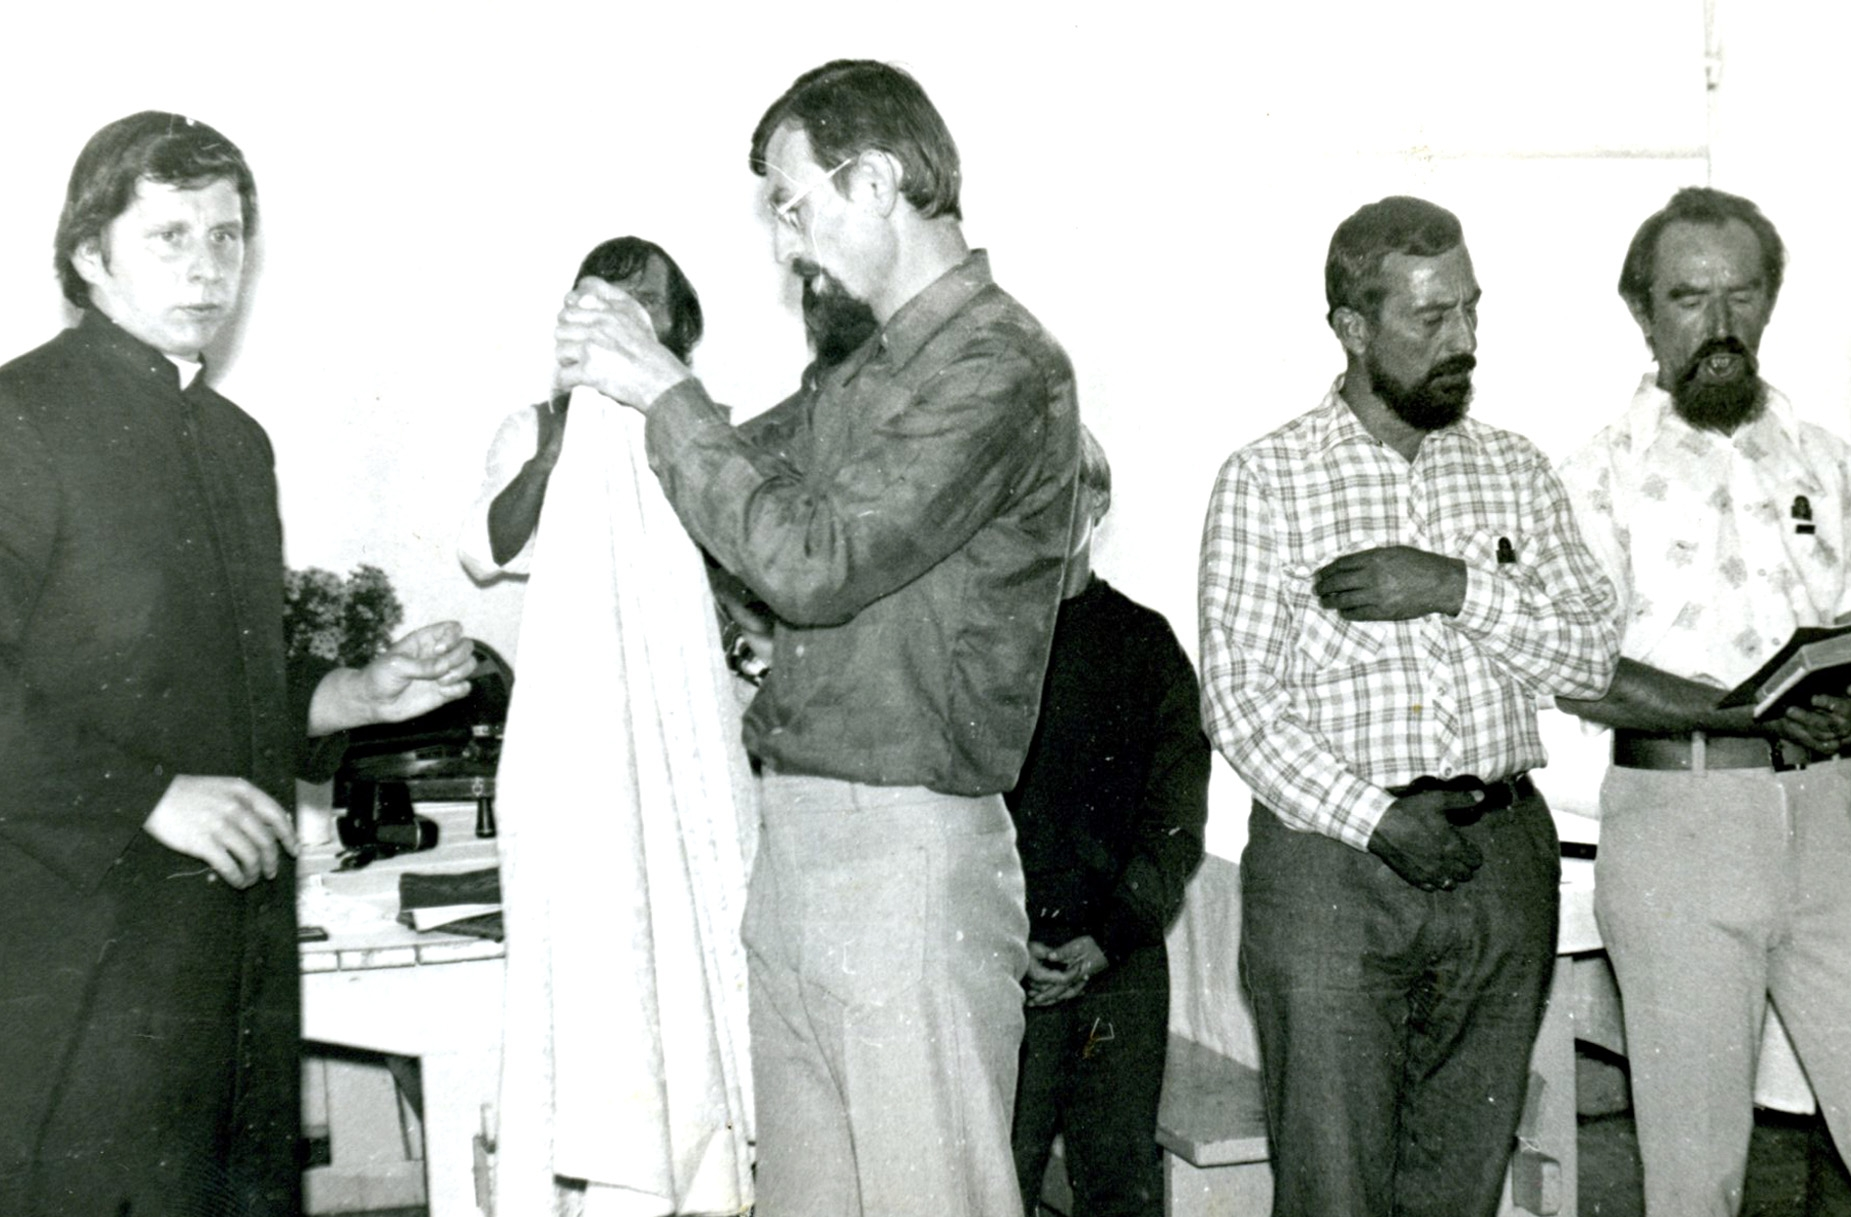
\includegraphics[width=0.6\textwidth]{photo/czeslaw_swierczynski_wiezienie_1.jpg}
\caption[Czesław Świerczyński w Uhercach Mineralnych]{Na zdj. Czesław Świerczyński z X. Rejdychem i Waldkiem Mikołowiczem w więzieniu w Uhercach Mineralnych}
\end{center}
\end{figure}

Szybko i mocno zżyliśmy się z naszymi kolegami z „Solidarności” Podkarpackiej, toteż gdy chciano ich wywieźć w nieznane, sprzeciwiliśmy się temu zamiarowi, barykadując łóżkami metalowymi wejście do naszego więziennego budynku, gdzie oni z nami byli uwięzieni. Suki odjechały tym razem bez nich. Wkrótce na takie dictum acerbum ubecja odpowiedziała prowokacją. Nasz więzienny kolega cierpiący na klaustrofobię kilkakrotnie chciał sobie odebrać życie. Gdy nareszcie, wg relacji współlokatorów jego celi, chciał się powiesić, co w ostatniej chwili udaremnili jego koledzy, a ubecja na zgłaszane do władz więziennych protesty odpowiadała jak zwykle propozycją współpracy, postanowiliśmy się zbuntować. Nadarzała się ku temu świetna okazja, gdy potężna cysterna z wodą stawała się z godziny na godzinę coraz bardziej pusta, aż dawała donośny, wręcz ogłuszający dźwięk. Koledzy owinąwszy sobie głowy jakby turbanem, by nie ogłuchnąć od tego cysternianego dzwonu, walili weń zapamiętale i na zmianę. Dźwięk był zaiste ogłuszający skoro w budynku przy zamkniętych oknach i drzwiach z wielkim trudem można się było, wrzeszcząc, porozumieć. Gdy już tak przez dobrą godzinę podzwoniliśmy sobie, jeden z kolegów, który po czasie okazał się prowokatorem, rzucił propozycję, by rozpalić wielkie ognisko! Ale czym palić? Niektórzy w tym buntowniczym nastroju poświęcili nawet swoje materace, krzesła...

Wtem co trzeźwiejsi koledzy zauważyli, że na „kogutkach”, tj. wieżyczkach strażniczych nie ma strażników, a zawsze tam byli, dzień i noc. Okazało się też, że w naszym budynku nie ma strażników, ba!, nie ma ich nawet na bramie głównej. Wtedy ów prowokator zawołał: „To uciekajmy!” Lecz wówczas najroztropniejsi, w tym Kaziu Trojan, powiedzieli stop! To może być prowokacja. A może komuna padła, a my tu niepotrzebnie siedzimy? Poszło kilku wtajemniczonych posłuchać radia ukrytego w maszynce do golenia. Po pół godzinie wrócili oznajmiając, że komuna niestety trzyma się mocno... To co robimy? Idziemy spać. Kilku niech pilnuje, co się będzie działo... W godzinę później, gdy się już zrobiło dobrze ciemno otoczyli nasze więzienie milicjanci, w pół godziny po nich zomowcy, w końcu późną już nocą przyjechali żołnierze. Wkrótce, to był koniec kwietnia, spadł śnieg, a ci żołnierze byli w letnim umundurowaniu. Było nam ich żal, bo przecież służby w wojsku nikt sobie w tamtych czasach nie wybierał, każdy zdrowy mężczyzna musiał dwa lata odsłużyć „ku chwale ojczyzny”. I tak całą noc stali, a myśmy smacznie spali, z wyjątkiem kilku czuwających.

Rano, około godziny ósmej zauważyliśmy formujące się przy bramie wjazdowej oddziały strażników więziennych. Co odważniejsi zgromadziliśmy się na spacerniku, by ich powitać naszą wiązanką pieśni patriotycznych, których w PRL-u nie wolno było śpiewać oraz pieśni antysowieckich i antykomunistycznych. Weszli i krokiem marszowym skierowali się ku naszemu budynkowi. Gdy byli już bardzo blisko podjęliśmy śpiew Mazurka Dąbrowskiego. Stał tam między innymi Rysiu Kuszłeyko, który wyraził zdziwienie, że tak mało nas na tym spacerniku. A oni nam namiętnie robili zdjęcia... Weszli do budynku. My za nimi, a tam tłum naszych, a więc nie spali, lecz czekali z podwiniętymi ogonami... Do pomieszczenia strażników, gdzie siedzieli ubecy, weszli dowódcy formacji otaczających przez całą noc nasze więzienie. I tam ku naszej satysfakcji podpułkownik czy może major rugał tych naszych ubeków używając najordynarniejszych słów, a myśmy jeszcze zza drzwi go zachęcali odzywkami w rodzaju: „a w ryja go”. 

Dzięki roztropności naszych kolegów najbardziej poturbowaną ciężkimi wyzwiskami okazała się ubecja... W kilka tygodni po tych zdarzeniach nasz internowany kolega wracający z przepustki do naszego więzienia był świadkiem rozmowy współpasażerów pociągu, w której mówiono o wielu ofiarach pacyfikacji naszego więzienia. Gdy zaś nasz kolega usiłował zdementować te hiobowe wieści jako autentyczny uczestnik tych wydarzeń, nie uwierzyli mu, a na okazaną im przepustkę z więzienia w Uhercach, uznali, że taką każdy ubek może sobie załatwić. Taki był wówczas stan gotowości bojowej narodu i absolutny brak zaufania do władzy ludowej. To wszystko zmarnował kabel Wałęsa i jemu podobni! Teraz ten kiedyś mężny naród jest ogłupiony, okradziony, oszukany, gotowy kalać własne gniazdo... \textbf{Oto potworne dzieło kapusiów w profesorskich togach, w sutannach, na ministerialnych i dyrektorskich stołkach...}

Gdzieś w końcu kwietnia w miejsce naszych kolegów z „Solidarności” krośnieńskiej, przemyskiej i rzeszowskiej osadzono kolegów z „Solidarności” kieleckiej i krakowskiej. Koledzy z Kielecczyzny: Edmund Sarna, Jurek Stępień i Stasiu Żak okazali się wspaniałymi przyjaciółmi, którzy wnieśli wiele dobra w życie naszej więziennej wspólnoty. Śp. Mundek Sarna parał się metaloplastyką wykorzystując blachę pozyskiwaną z konserw, Jurek Stępień grywał nam na saksofonie i gitarze, a Stasiu Żak dawał fenomenalne wykłady z historii literatury opatrując je cytatami z pamięci, niejednokrotnie budzącymi podziw częstotliwością i obszernością. Słuchało się go z ogromną przyjemnością, a znajomość z nim przetrwała aż do późnych lat 90’. Był on senatorem przez dwie pierwsze kadencje zaś Jurek Stępień jest sędzią Trybunału Konstytucyjnego.

Natomiast koledzy z Regionu Małopolskiego mieli jakiegoś przywódcę bardzo niezrównoważonego, który wzywał nas do permanentnego buntu przeciw władzy więziennej jako substytutu władzy państwowej, a efektem tego buntu powinna być ruina tego więzienia, z którego nie powinien pozostać kamień na kamieniu. Pewnie to on właśnie co pewien czas wieczorami i nocą na całe gardło wrzeszczał „alarm!”, aż wreszcie spotkał się z zapowiedzią jednego ze współwięźniów, który onegdaj odsiedział wieloletni wyrok za zabójstwo w afekcie, że gotów jest odsiedzieć drugie tyle za uciszenie na zawsze tego, który ryczy po nocy idiotyczne alarmy. Poskutkowało, ale zamiast tego w ramach buntu nasrał w nocy na skrzyżowaniu korytarzy więziennych. A gdy i to spotkało się z nasza dezaprobatą owi buntownicy wszystkie śmieci wyrzucali przez okno zamiast do kosza, tak że po pewnym czasie można było bez trudu wskazać celę należącą do nich. Był to dla nas – działaczy „Solidarności” wielki wstyd, kompromitacja naszego ruchu!

Od 13 marca przyjęło się obchodzić miesięcznicę naszego internowania. W związku z tym zaproponowałem kolegom, by 13 maja odstąpili od tego zwyczaju ze względu na pierwszą rocznicę zamachu na Jana Pawła II i w podzięce za uratowanie mu życia odmówili „Anioł Pański”. Koledzy jednak nie chcieli słyszeć o tym, by miesięcznicę swojej było nie było klęski zastąpić dziękczynieniem w rocznicę zwycięstwa Maryi nad skrytobójczym zamiarem mocodawców Ali Agcy. Anioł Pański odmawiałem tylko ja z Waldkiem Mikołowiczem.
\begin{figure}[!h]
\begin{center}
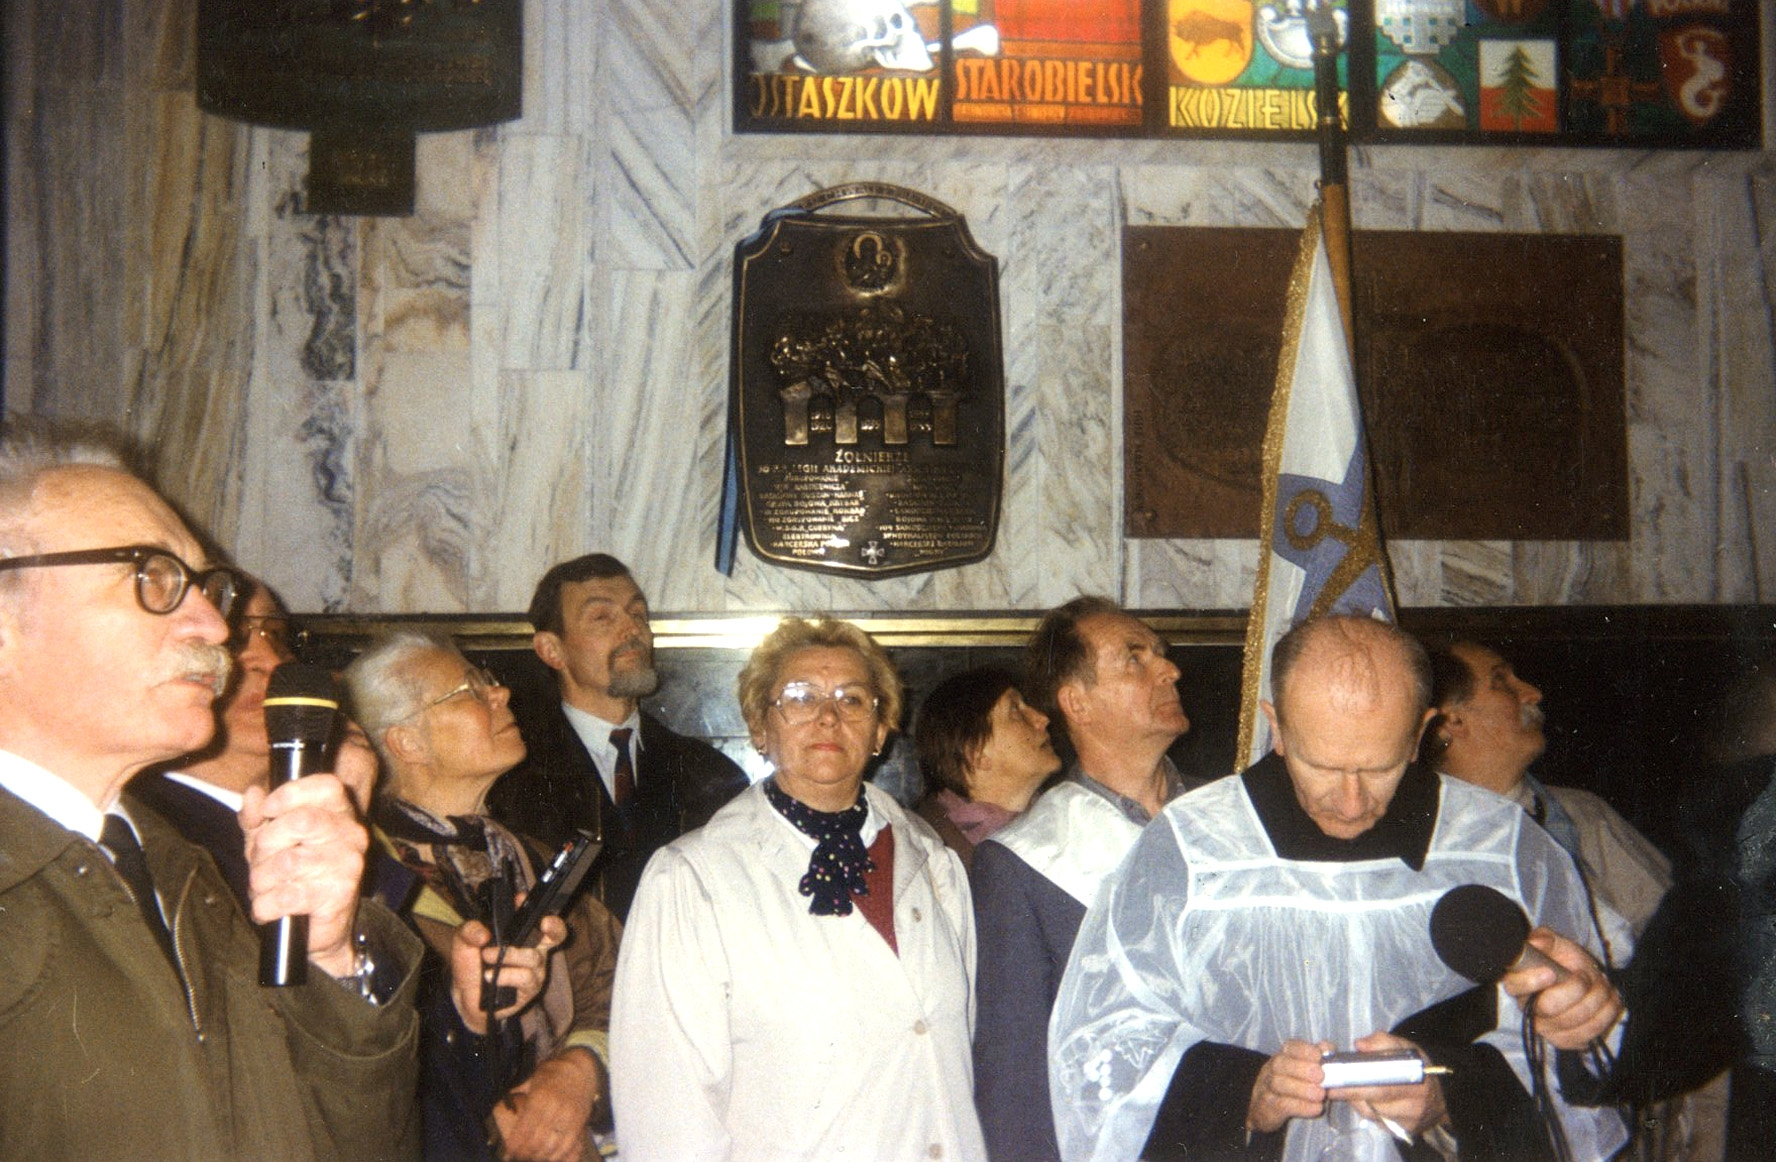
\includegraphics[width=0.6\textwidth]{photo/jasna_gora_uroczytosci_katynskie.jpg}
\caption[Uroczystości Katyńskie na Jasnej Górze]{Uroczystości Katyńskie na Jasnej Górze. Sztandar dzierży Waldek Mikołowicz, Ja stoję w głębi}
\end{center}
\end{figure}

Reszta świętowała... swoje uwięzienie. W tydzień później od Kazia Trojana dowiedziałem się, że właśnie 13 maja urodził mi się syn – ma się rozumieć – Bożydar. Wielki jest Bóg, który w szczodrobliwości nie pozwoli się prześcignąć człowiekowi. Podła ubecja telegram o narodzinach Bożydara dostarczyła mi w ostatnich dniach maja, kiedy na interwencję bpa Bednorza otrzymałem przepustkę na chrzest mojego syna. Ubecja była zdolna do jeszcze większej podłości. Oto telegram o śmierci rodziców naszego kolegi, którzy zginęli w wypadku samochodowym, przekazali mu wiele dni po ich pogrzebie.

Pomimo sugestii mojej Mamy i wcześniejszej sugestii własnej czy też Ducha Świętego, by chrzestnymi ustanowić Jasia Wilczka i Basię Wilk wpadłem na pomysł, by chrzestną Bożysia była Zosia Prele, gdyż w ten sposób niejako chciałem włączyć Zosię na powrót do rodziny jako odrzuconą przez społeczność rodzinną. A przecież chrzestnych się wybiera dla swego dziecka, a nie dla uzdrawiania stosunków rodzinnych! Bóg jednak, pomimo tych moich błędów czuwa nad Bożydarem i wielkie mu za to dzięki! Na chrzcie Bożydara było więcej niż zwykle osób duchownych. Była ciocia Aurelia Świerczyńska, był ojciec Oskar Puszkiewicz wraz z ówczesnym prowincjałem franciszkanów – Damianem Szojdą. A dziadek Benedykt – wtedy jakże zagorzały zwolennik WRON-y i Jaruzelskiego miał pełne spodnie strachu, bo skądże u niego tyle osób duchownych, niech to jakiś kapuś doniesie...

Pewnie w czerwcu przybyła do nas delegacja Międzynarodowego Czerwonego Krzyża. Znalazło się kilku kolegów znających dobrze francuski, którzy tłumaczyli nam, to co mieli nam do powiedzenia ci dygnitarze, a trzeba przyznać, że spodziewaliśmy się wiele po tej wizycie. Po wstępnych kurtuazjach zakomunikowaliśmy im, że znaczna część pomocy, jaka przychodzi od nich dla nas, jest zawłaszczana przez SB i cały aparat represji, o czym świadczy m.in. fakt paradowania strażników więziennych tego więzienia w ubraniach przysłanych dla nas z Finlandii i że w tej sytuacji domagamy się z ich strony interwencji. Na to oskarżenie i żądanie wypowiedziane przez nas w obecności komendanta więzienia i oficerów SB szef owej delegacji odpowiedział, że oni nie mają tu żadnej władzy i nie będą w tej sprawie interweniowali, bo za tą władzą stoi cały Związek Sowiecki. Po tej wypowiedzi nastało przejmująco długie milczenie. Lepiej, by w ogóle nie przyjeżdżali, niż mieli nam coś takiego powiedzieć. Zgniły Zachód już wtedy był przeniknięty agenturą komunistyczną i drżał na samą myśl zbrojnej „wizyty” Sowietów w ich sytych ojczyznach...

Na początku czerwca, dzięki interwencji bpa Bednorza, wyszedł na wolność Kaziu Trojan żegnany przez nas bardzo uroczyście. Od tego czasu utarł się zwyczaj żegnania piosenką każdego internowanego wychodzącego na wolność. Tak było do 22 lipca. Po tym święcie podwójnej zdrady narodowej (najpierw Stanisława Poniatowskiego z targowiczanami i kurtyzaną Katarzyną w 1792 r., a następnie tzw. Rządu Lubelskiego ze Stalinem w 1944 r.) nastąpiły tak masowe wypuszczenia, że wkrótce nie było komu grać i śpiewać piosenek pożegnalnych. W ostatnich dniach lipca każdy miał do dyspozycji całą celę. Tyle nas zostało. I wtedy ów Ciepiela, z którym siedziałem w jednej celi w Raciborzu zadrwił ze mnie, że tyle modlitw moich na darmo, że Pan Bóg widać głuchy na moje wołanie. 

Gdyby on wiedział jak ja sobie porozmawiałem z moim ubekiem, to by się pewnie nie dziwił, że mnie władza ludowa nadal pozostawiła w więzieniu z adnotacją, by mnie trzymać w odosobnieniu do końca stanu wojennego. A wszystko dlatego, że mu wyłuszczyłem czarne na białym, że ich postępowanie jest bezprawne, nielegalne, że komuna robi bokami i że nie minie dziesięć lat, gdy upadnie... Facet się bardzo na mnie wkurzył, wrzeszczał, nawet wyjął z kabury rewolwer i mówi do mnie, że gdybym wystąpił o zmianę  decyzji o internowaniu to może dałoby się coś zrobić. A ja mu na to, że odwoływanie się w tych warunkach byłoby jednoznaczne z uznaniem bezprawia jakiego się ta władza dopuściła. W sumie przez tę rozmowę zarobiłem drugie sześć miesięcy...

W pierwszych dniach sierpnia wywieźli nas do więzienia w Rzeszowie Załężu. Tam ponownie spotkałem Włodka Forysia – ekonomisty, pracownika naukowego Politechniki Śląskiej oraz Waldka Mikołowicza. Tam po raz drugi odczułem, że jestem przez środowisko odrzucony, ponieważ nikt mi nie zaproponował zamieszkania z nim w celi. W takiej samej sytuacji znalazł się także Rysiu Kuszłeyko, Tadek Dudek oraz Kaziu Cieśla, więc zamieszkaliśmy razem w jedynej celi czteroosobowej i od tej pory mieszkaliśmy już razem aż do zwolnienia z internowania, a więc także w Nowym Łupkowie.

Tam do więzienia w Rzeszowie Załężu obiecał przybyć w święto Matki Bożej Jasnogórskiej ordynariusz częstochowski – śp. bp Stefan Bareła. Do tego niebywałego wydarzenia poczyniliśmy stosowne przygotowania. Jakież było nasze zdziwienie, gdy rano 26 sierpnia nasze cele zastaliśmy po raz pierwszy zamknięte. Zaczęliśmy walić w drzwi czym popadło, a w większych celach – ośmioosobowych, ponieważ nie wszyscy mogli dorwać się do drzwi, w jednej z nich koledzy wpadli na pomysł, by metalowym łóżkiem walić w ścianę boczną celi. Jakież było ich zdumienie, gdy po kilku uderzeniach ściana się rozsypała, za którą ujrzeli zaskoczonych kolegów z sąsiedniej celi, którzy wkrótce pokonali następną ścianę , a za nią następną i następną, aż dotarli do niezamieszkanej celi, która z tego powodu nie była zaryglowana. Najszczuplejsi przedostali się do niej i wydostawszy się na korytarz pootwierali wszystkie nasze cele, gdyż strażnicy więzienni, nie chcąc słuchać wywołanego przez nas hałasu, opuścili nasze piętro. Wylegliśmy wszyscy na korytarz pełni oburzenia na władze więzienne, ale też mocno podekscytowani wyjątkowym obrotem sprawy. Kraty oddzielające korytarz od klatki schodowej opierały się tylko kilka minut przed naszym naporem i tak w chwilę później znaleźliśmy się pod drzwiami naczelnika więzienia. Naczelnik nie miał odwagi wyjść do nas, bo też wyzywaliśmy go od najgorszych, że nam zepsuł takie święto! Wieczorem wywieźli nas sukami do Nowego Łupkowa.

W drodze do kolejnego więzienia koledzy opowiadali, że spod tynku niektórych rozwalonych łóżkami ścian ukazały się wiązki przewodów do podsłuchu więźniów, lecz najistotniejsza była zagadka tajemniczej słabości ścian działowych między celami. Czy to cud, czy może efekt naszego wyjątkowego wzburzenia, czy też może ściany tych naszych cel tak zostały wymurowane, że mogły się rozpaść pod każdym silniejszym uderzeniem. Koledzy istotnie widzieli jak licha była zaprawa wiążąca cegły rozwalonych ścian. Ktoś więc kradł cement przeznaczony na budowę rzeszowskiego więzienia, a więzienie było budowane w PRL-u i to przez samych więźniów. Lecz to nie więźniowie ukradli ów cement, a jacyś strażnicy więzienni lub może sam komendant więzienia. Skoro więc już sam aparat sprawiedliwości przeżarty był rakiem korupcji i oszustwa, to przecież ustrój socjalistyczny musiał mieć się ku końcowi. Ja wróżyłem mu upadek w ciągu dziesięciu lat, na co mam świadków. Pomyliłem się, ustrój upadł szybciej, lecz nie pod ciosami „Solidarności”, a w wyniku pazerności niedawnych towarzyszy PZPR chciwych majątku państwowego, który uważali za niczyj, a więc nadający się do rozgrabienia! \textbf{I tak po 89’ byliśmy świadkami grabieży majątku narodowego na niespotykaną skalę!!! A kradli nie zwykli złodzieje, lecz złodzieje z tzw. klasą polityczną...}

W Nowym Łupkowie było nam najlepiej. Wprawdzie wróciły chłody, ale w każdej celi były powłączane nasze domowe grzejniki, więc nie było nam zimno, a ponadto przychodziło do nas tyle różnych darów, że nie można było tego przejeść zatem ich część przekazywaliśmy rodzinom na widzeniach. W związku z tym powstało dowcipne pytanie w naszym więzieniu: Po czym można odróżnić rodziny więźniów kryminalnych od rodzin internowanych? Po tym, że te pierwsze wchodzą z pełnymi torbami a te drugie wychodzą objuczone darami.

Do Nowego Łupkowa trafiliśmy 27 sierpnia nocą. Niewiele więc mieliśmy czasu, by zorganizować obchody drugiej rocznicy powstania NSZZ „Solidarność”. Postanowiliśmy zawiesić na wysokiej na 20 m latarni białą flagę z charakterystycznym czerwonym napisem „Solidarność”. Flagę wykonał Waldek Mikołowicz, którego warsztat drukowania tkanin i papieru pracował do późnych godzin nocnych, dzień w dzień, tak że z powodu chronicznego niedosypiania jego szef miał kłopoty z sercem. Flaga wysuszona czekała więc 31 sierpnia na śmiałka, który zawiesi ją na owej latarni. Uczynił to wczesnym rankiem Tadek Dudek – niezwykle sprawny fizycznie student V roku matematyki. Flaga łopotała radośnie od rana nad całym naszym więzieniem, a pod latarnią jak masztem przeprowadziliśmy uroczysty apel ze śpiewami zakazanych pieśni patriotycznych. 

Wkrótce zjawił się u nas komendant więzienia z żądaniem byśmy zdjęli tę naszą flagę. Oczywiście spotkał się z negatywną odpowiedzią. Komendant zrozumiał, że sam będzie musiał ją zdjąć, ale jak to zrobić bez „zwyżki”, czyli drabiny mechanicznej? Sprowadzenie jej z Rzeszowa odpadało, gdyż trzeba byłoby się przyznać do niedostatecznego sprawowania nadzoru nad więźniami! Wobec takiego dictum acerbum pan komendant pofatygował się do nas ponownie z propozycją polubownego załatwienia sprawy. Koledzy wytargowali od niego sporo ułatwień w naszym więziennym życiu, tj. udostępnienie za dnia całego obszaru więzienia dla internowanych, była swoboda wychodzenia z baraku więziennego przez cały dzień, była swoboda rozmów podczas widzeń z rodzinami... Gdy zaś komendant spróbował się wycofać z tych swoich zobowiązań i zamknął nas w naszym baraku, wówczas nauczeni doświadczeniem rzeszowskim wywaliliśmy łóżkami metalowymi okno korytarzowe, przez które wyszliśmy na zewnątrz i dotarliśmy do komendanta, by go zapytać o obyczaj dotrzymywania słowa. Więc już się incydent z zamykaniem baraku nie powtórzył. Dopiero ucieczka Antka Macierewicza z więzienia sprawiła, że na noc zamykano nasze baraki więzienne.

Wielkie wzburzenie wywoływało we mnie opalanie się niektórych naszych kolegów całkiem nago z wywalonymi bezwstydnie genitaliami. Oburzało nas to nie tylko ze względów religijnych, ale także w trosce o naszą opinię. Przecież władze więzienne mogły bez trudu sfotografować tych błaznów i wysłać zdjęcia do ich Komisji Zakładowych NSZZ „Solidarność” i opublikować je w reżimowej prasie! Tego tylko nam jeszcze brakowało. Całe szczęście skończyły się ciepłe dni, a wraz z nimi warunki do opalania. Ta nonszalancja wielu internowanych pozwoliła przefarbować się komunistom we właścicieli mediów, zakładów pracy, uczelni itd. We Mszy św. niedzielnej, którą odprawiał ksiądz z Łupkowa uczestniczyło mniej niż jedna trzecia kolegów, mimo że w pantoflach mogli na nią przyjść, bo się odprawiała za ścianą ich celi! Nic więc dziwnego, że taka „Solidarność” dała się łatwo omotać, wciągnąć w lewe interesy i wykorzystać jako agentura SB.

W Łupkowie szła na całego produkcja zakazanej bibuły, znaczków poczty więziennej, makatek z Mickiewiczowskim dwuwierszem \textbf{\textit{„Tylko pod krzyżem, tylko pod tym znakiem, Polska jest Polską, a Polak Polakiem”}}. Tutaj też nagrywaliśmy dla rodzin śpiewane przez nas zakazane i patriotyczne piosenki, rozpoczynające się „Bogurodzicą”. Od początku grudnia rozpoczęły się liczne wyjścia kolegów na wolność. Naszą celę opróżnili jednego dnia, tj. 11 grudnia, Najpierw wyszedł Tadek Dudek, potem Rysiu Kuszłeyko, na końcu autor tych wspomnień. Ze względu na późną porę otrzymania decyzji o zwolnieniu z internowania mogłem jedynie dojechać do Zagórza i tam czekać do rana na pociąg do Katowic albo też zatrzymać się u sióstr w słynnej Komańczy – ostatniego miejsca internowania Prymasa Tysiąclecia – Stefana kardynała Wyszyńskiego – interrexa. Oczywiście nocowałem u sióstr, by we wczesnych godzinach niedzielnych ruszyć pociągiem wprost do Częstochowy – na Jasną Górę najpierw podziękować Matce Bożej i Królowej Polski za uwolnienie z więzienia i za moją rodzinę, za Zuzię i za Bożydara. Zdążyłem na Prymarię, na Mszę św. odpustową z 8 grudnia – Niepokalanego Poczęcia Najświętszej Marii Panny. \textbf{A potem powrót do domu, na Strażacką i wielka radość półrocznego Bożysia, że gdyby umiał, to by z wózka dziecięcego wyskoczył!}

Potem powrót do pracy, do Huty „Katowice”, lecz tu zaskoczenie – mam do wybrania dwa miesiące urlopu, więc dopiero w lutym mogę podjąć pracę. I zamiast czas ten przeznaczyć na jakieś remonty, na rozmowę z rodziną, co dalej robić, zacząłem szukać zatrudnienia w szkolnictwie... Nie konsultując swej decyzji z nikim zwolniłem się z Huty Katowice i zatrudniłem w Domu Chłopców prowadzonym przez siostry zakonne. Starałem się wywiązywać z moich obowiązków jak najlepiej... Jakież było moje zaskoczenie, gdy w czerwcu otrzymałem od siostry dyrektor wypowiedzenie z pracy bez podania istotnych przyczyn. Nie była to jednak szkoła podległa Ministerstwu Oświaty i Wychowania, więc decyzja siostry dyrektor nie mogła być podważona. Zostałem bez pracy. Wcześniej, tj. w okolicach 13 maja obchodziliśmy roczek Bożydara na Jasnej Górze z obiadem dla gości, wśród których była także babcia Zofia, wujek Walery z ciocią Ritą, Wilki, chrzestni Mirosław Głąb i Zosia Prele. Staliśmy przed samym obrazem Matki Bożej Jasnogórskiej – Królowej Polski. O przewiezienie nas na Jasną Górę poprosiłem Zbyszka Nowakowskiego, którego pomawiano o kontakty esbeckie, ponieważ kiedyś był taksówkarzem, na co koncesję wydawało SB. Może i prawda, ale ja wiele od niego skorzystałem, a zwłaszcza w uroczystość „Roczku” Bożydara, kiedy to mamusia jego tak bardzo się grzebała przy nim i ze sobą, że nam na dotarcie z Myszkowa na Jasną Górę zostało niewiele ponad pół godziny. Tylko dzięki jego niezwykłym umiejętnościom i Matce Bożej byliśmy tam w 25 minut, niemal stale jadąc z prędkością znacznie przekraczającą 100 km/godz. Na Jasnej Górze o tej porze, tj. o 11 w majową niedzielę tłok i tylko dzięki mojej znajomości tajemnych przejść dotarliśmy w pięć minut do zakrystii, gdzie wszyscy goście już czekali wraz z Ojcami Paulinami wstrzymywanymi heroicznie przez cudowną panią Martę Wójcik, mimo że już było po czasie rozpoczęcia Mszy św. To Matka Boża czuwała nad Twoim „Roczkiem” kochany Bożydarze i okazała się nad wyraz skuteczną. Po Mszy w intencji Bożydara zostaliśmy przez panią Martę Wójcik oprowadzeni po Skarbcu Jasnogórskim poza kolejnością i ze szczególnie bogatym w treść komentarzem przewodnickim. Potem powrót trzema samochodami na kawę do Myszkowa.

Dzięki pani Marcie Wójcik wyjechaliśmy też na wczasy do Gdyni, które nam zafundowała pani Wanda Okońska u krewnych swojej rodziny. Załatwiła nam też pani Marta Wójcik, która prowadziła na Jasnej Górze poradnię psychologiczną, miejscówki na przejazd pociągiem pośpiesznym do Gdyni, o co wówczas było bardzo trudno. W dniu wyjazdu Bożyś nagle się rozchorował i trzeba było wyjazd odłożyć, a miejscówki przepadły. O uzyskaniu nowych nie było co marzyć. Wymyśliłem więc przelot samolotem do Gdyni, który okazał się moim jedynym lotem, a pierwszym dla Zuzi i Bożydara.

Do pracy zatrudnił mnie nasz kuzyn, późniejszy chrzestny Piotrusia – Krzysiu Karoń i płacił mi uczciwie także ZUS. Starałem się wywiązywać ze swoich obowiązków. Uczył mnie Krzysiu jeździć traktorem i gdybym był wytrwały, to pewnie bym już dzisiaj jeździł samochodem. Lecz gdy przydarzyło mi się nakarmić gęsi zaprawionym ziarnem, którego worek stał w pobliżu worków z ziarnem jadalnym, co niektóre z nich nie przeżyły a wszystkie odchorowały, zrezygnowałem z pracy u Karoniów, w czym nie ma ich winy. Jedynie mój brak pokory i wytrwałości sprawił, że się stamtąd oddaliłem. 

Od nowego 1984 roku zaangażował mnie na stanowisko katechety ks. Marian Gołąbek. To była jego wielka odpowiedzialność, której podjął się pod namową Józefa Lamcha, niezwykle odważnego i niespożytego działacza „Solidarności Rolników Indywidualnych”. To działanie Opatrzności Bożej, która zamiast soczystego klapsa dała mi nową szansę! Przecież ja nie miałem żadnego przygotowania katechetycznego, które uzyskałem dopiero podczas dwumiesięcznego kursu w Instytucie Teologicznym w Częstochowie. Za odwagę zaangażowania mnie do nauki religii drogo zapłacił proboszcz parafii Najświętszego Serca Jezusowego w Sokolnikach. Ubecy rozpuścili pogłoskę o rzekomym gwałcie homoseksualnym na młodym mieszkańcu Dobrogoszczyc, który wraz ze swą narzeczoną dał właśnie na zapowiedzi o zamiarze zawarcia małżeństwa. Gdy się o tym dowiedziałem, natychmiast udałem się do rzekomej ofiary gwałtu, gdzie był wielki lament z powodu wstydu, jaki mu zrobiła ubecja puszczając w świat kompromitujące kłamstwo. To była ohydna zemsta ubecji za wykazanie przed sądem, że wybory do sejmu na terenie gminy Niegowa zostały sfałszowane, gdyż do lokali wyborczych przybyło tam znacznie mniej obywateli niż podano do wiadomości. Ksiądz Marian Gołąbek widząc z jaką szybkością rozniosła się wieść o jego rzekomym gwałcie i jak parafianie dali jej wiarę, postanowił opuścić nie tylko swoją parafię, ale ojczyznę i osiadł jako misjonarz w Kanadzie.

Wyjeżdżamy na darmowe wczasy w góry, do Mszany Dolnej, do rodziny stolarza Józefa i kucharki Marii Aksamitów. Opłacaliśmy jedynie nasze wyżywienie. A przecież oni mieli już wtedy pięcioro dzieci (Pawła, Urszulę, Magdę, Roberta i Monikę, która zginęła przejechana przez samochód, co dzielni rodzice powetowali sobie wkrótce Wojtkiem i Pauliną)! To są do dzisiaj wspaniali ludzie. On mężny i przedsiębiorczy, ona pracowita i wierna. Pełni humoru i wielkiego serca i bardzo, bardzo gościnni. Byliśmy tam wiele razy, zawsze serdecznie witani. Bywaliśmy tam zimą i latem. Był tam też raz Rafałek Jabłoński.
\begin{figure}[!h]
\begin{center}
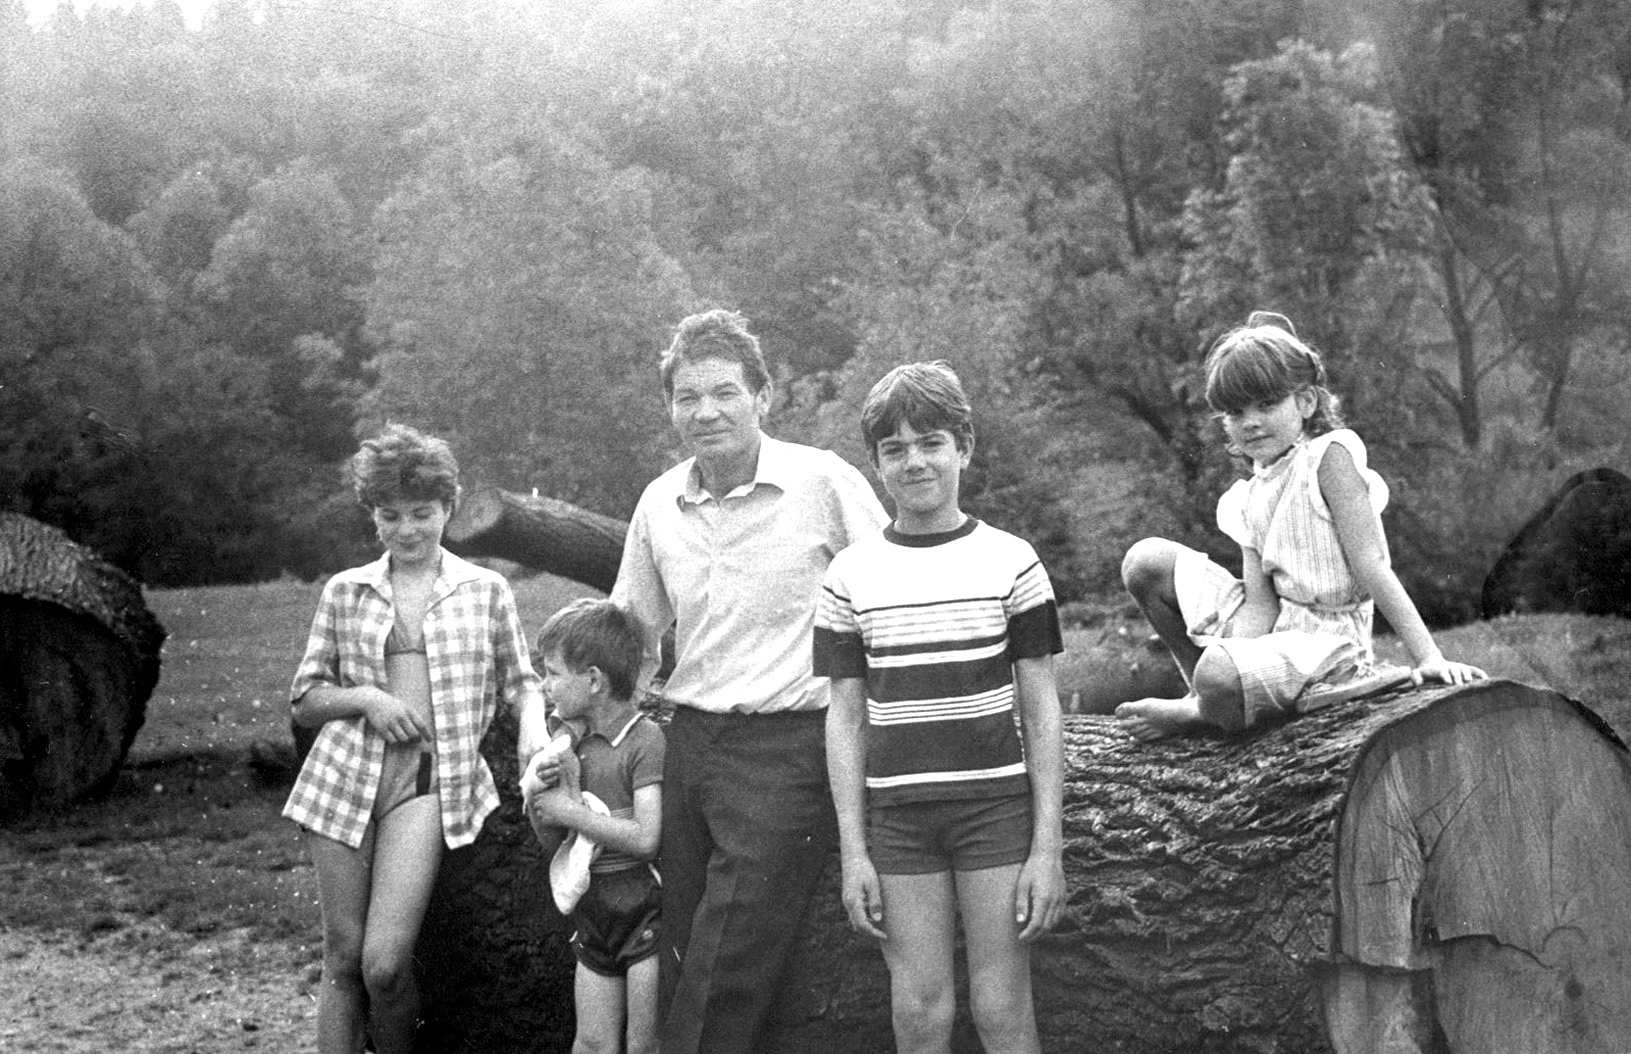
\includegraphics[width=0.6\textwidth]{photo/rodzina_aksamitow.jpg}
\caption[Rodzina Aksamitów]{Na zdj.: Urszula i Robert Aksamitowie, ich ojciec Józef Aksamit, Paweł i Magda Aksamit.}
\end{center}
\end{figure}

Dzięki wstawiennictwu wówczas księdza doktora, dziś biskupa Antoniego Długosza, wykładowcy na kursie katechetycznym, zatrudnił mnie ksiądz prałat Zygmunt Sroka na pełny etat w parafii Matki Bożej Królowej Polski w Zawierciu. Katechizowana tam przeze mnie młodzież była bardzo trudna, w dodatku inspirowana negatywnie do mnie przez SB, co można wyczytać z doniesień jakichś TW na temat moich katechez, które – trzeba powiedzieć – były odważne, chociaż wyważone. Niestety, w 1987 r. sam się zwolniłem z tej pracy i to tak nieroztropnie, że okazało się we wrześniu, iż nie mam żadnej pracy. Dopiero w październiku zostałem zatrudniony w Kopalni Węgla Kamiennego Boże Dary w Katowicach Kostuchnie. Tam pracowałem na oddziale wentylacji i trafiłem na wspaniałych kolegów, zwłaszcza na Mariana Uszoka, który mnie bardzo życzliwie wprowadzał w arkana pracy. Zginął na krótko po moim odejściu z kopalni do pracy w szkole. Mam takie przeczucie, że gdybym nadal pracował w kopalni to pewnie na mnie wpadłby ów wóz kopalniany, który zmiażdżył Mariana... Gdy Marian umarł nagle zaświeciła się nadzwyczajną jasnością niewłączona do prądu żarówka! Zaraz tego dnia pojechałem do szpitala górniczego w Sosnowcu, ale mnie do niego nie wpuszczono. Dowiedziałem się jednak, że zmarł dokładnie o tej godzinie, o której zaświeciła się i eksplodowała owa żarówka.

Tego dnia był przeprowadzony konkurs na stanowisko kuratora oświaty, na którym się nie pojawiłem, a miałem szansę go wygrać, ponieważ prowadził go Jarek Kapsa! Kolejna szansa dana mi przez Opatrzność zmarnowana przez moje otumanienie! Potem w czerwcu były pierwsze wolne wybory do Rad Gmin. Gdybym wszedł do Rady Miasta Myszkowa byłbym został jego burmistrzem, ale gdy wszystko precyzyjnie zorganizowałem, tak że w Radzie mieliśmy zdecydowaną większość, ja się wyznaczyłem do obwodu Zygmunta Ratmana, będąc głupio przekonany, że wszyscy będą głosowali na mnie. Przegrałem z kretesem!... W kilka miesięcy później wygrałem z E. Bugajem konkurs na dyrektora delegatury Kuratorium Oświaty w Myszkowie, którym byłem przez trzy lata. Moim szefem był Włodzimierz Kolman, człowiek publicznie przyznający się do tego, że nie zna prawa oświatowego, a jednocześnie prowadzący narady po osiem i więcej godzin, które można było zmieścić w dwóch godzinach. Człowiek, który wyleciałby ze stanowiska, gdyby nie upadek rządu Olszewskiego!

To dzięki moim zabiegom przestał być dyrektorem szkoły w Dąbrownie Eugeniusz Stecz, wyjątkowa kreatura, pijak, chuligan, ordynarny w obejściu z dziećmi i z kobietami. Gdyby nie jakieś wyjątkowe poparcie w MEN i w naszym kuratorium w osobie pani Rzepki, już dawno przestałby być nie tylko dyrektorem, ale i nauczycielem. Jednak dalej jako nauczyciel uprzykrzał życie nowej pani dyrektor i gdy wreszcie przyłapały go panie nieprzytomnie pijanego, wiszącego wpół na barierce szkolnej i pobrały z pomocą policji krew zawierającą ponad dwa promile alkoholu, wówczas przyszła mu z pomocą pani Rzepka. Oto jedynie w zawodzie nauczycielskim pijaństwo tolerowane jest na tyle, że za pojawienie się w godzinach pracy w stanie wskazującym na spożycie alkoholu może o karze orzec dopiero komisja dyscyplinarna, której przedstawia się dokumenty poświadczające takie czy inne wykroczenie nauczyciela. Te dokumenty jakoś zaginęły pani Rzepce i odnalazła je dopiero, gdy się owo wykroczenie Stecza przedawniło! Pani Rzepce włos z głowy za to nie spadł, ja natomiast miałem mnóstwo kwasów ze strony Kolmana, który musiał się za owego pijaka tłumaczyć w MEN. Doprowadziłem jednak w końcu do tego, że E. Stecz przestał być nauczycielem i handlował owocami na targowisku w Myszkowie, do czego pewnie się znacznie bardziej nadawał, a przynajmniej nie deprawował dzieci!

Podobnie trudną sytuację miałem z dyrektorką szkoły w Markowicach (obecnie nieistniejącej), żoną ówczesnego burmistrza Miasta i Gminy Koziegłowy M. Szczęsnego, kobiety niezrównoważonej psychicznie, mającej rujnujący wpływ na dzieci klas I – IV i nauczycieli tam uczących. Wobec tego  zarządziłem wizytację tej szkoły i powiadomiłem o tym panią dyr.  E. Szczęsną. Jakież było nasze zdziwienie, gdy w dniu wizytacji nie zastaliśmy w szkole pani dyrektor, nauczyciele po godzinie rozpoczęcia zajęć dopiero schodzili się do szkoły a dzieci pod opieką woźnej czy sprzątaczki biegały po budynku szkolnym!.. Od pierwszej napotkanej nauczycielki zażądaliśmy udostępnienia dzienników i innej dokumentacji szkolnej. Nie udostępni, bo wszystko jest pozamykane. W końcu dotarł do szkoły ksiądz, który w samych superlatywach wypowiadał się o pracy pani dyrektor. Po wizytacji wracamy z panią dyrektor SP w Koziegłowach do Myszkowa i mija nas ów ksiądz, na co wyraziłem zdziwienie, gdyż wg planu powinien jeszcze katechizować. Na co zaskoczona pani dyrektor oświadczyła, że to żaden ksiądz, tylko syn pani Szczęsnej. Wracamy! W~szkole zastajemy tym razem prawdziwego księdza. W związku z próbą oszustwa składam wniosek o zdjęcie pani Szczęsnej z funkcji dyrektora SP w Markowicach. Wniosek po wielu utarczkach został w końcu przyjęty i pani dyrektor odeszła na wcześniejszą emeryturę.

Obszar mojej delegatury sięgał wówczas aż za Szczekociny, po Moskorzew, obejmował także gminę Włodowice i cały obecny powiat myszkowski. Gdy MEN zażądał od kuratora Kolmana likwidacji trzech spośród pięciu delegatur w ówczesnym województwie częstochowskim, wówczas na pierwszy ogień poszła delegatura myszkowska. W tej sprawie pojechałem do MEN, do Warszawy wyposażony w list polecający senatora Stanisława Żaka. Pani wiceminister nie chciała się zgodzić na pozostawienie delegatury myszkowskiej kosztem jakiejś innej, lecz zaproponowała mi mediację w mojej sprawie, by mnie kurator zostawił u siebie na stanowisku wizytatora, lecz ja się na to nie zgodziłem. To była moja kolejna życiowa głupota! Pozostał mi powrót do Zespołu Szkół Zawodowych, gdzie dyrektorowała pani Jadwiga Górniak, która - za ujawnienie przeze mnie jej haniebnych praktyk przy przyjmowaniu dzieci ze szkół podstawowych – serdecznie mnie nienawidziła i robiła wszystko, by mnie nie przyjąć do szkoły. Było to bezprawne działanie, więc mnie Sąd Pracy wziął w obronę, a przecież mogłem tego wszystkiego uniknąć, gdyby we mnie było trochę więcej pokory i rozumu...

Jako polonista i zarazem katecheta, a także prezes Akcji Katolickiej w parafii pw. św. ap. ap. Piotra i Pawła miałem możliwość załatwienia dla całej mojej rodziny wejściówki na Jasną Górę, ale brakło mi odwagi i załatwiłem ją tylko dla siebie i waszej Mamy. Wybrałem się jednak wówczas na Jasną Górę z moimi chłopakami, których służby specjalne nie zechciały wpuścić i w ten sposób mając szansę być bardzo blisko Ojca Świętego Jana Pawła II Wielkiego, utraciłem ją bezpowrotnie, gdyż ks. bp Antoni Długosz miał pretensje do mnie, że się nie zjawiłem wówczas na Jasnej Górze...

W tamtych czasach niepodzielnie rządziła lewica wespół z kapusiem, tj. kablem Wałęsą, a później pod przewodem pseudomagistra Aleksandra Kwaśniewskiego – pijaka, więc pani Górniak mogła się mnie nie bać. Przyszedł jednak czas, kiedy zostałem przewodniczącym Porozumienia Samorządowego „Razem” i w wyborach samorządowych 1998 r. wszedłem do Rady Miasta Myszkowa. W 1999 r. jeszcze częstochowskie Kuratorium Oświaty oświadczyło pani Górniak, że nie przedłuży jej kadencji na kolejne pięć lat oraz że ogłosi konkurs na stanowisko dyrektora. Wówczas kuratorem była moja koleżanka – Anna Pawłowska i gdybym zadbał o opinię we właściwym terminie u pani dyrektor, wówczas wygrałbym ten konkurs. O opinię wystąpiłem na kilka tygodni przed konkursem, lecz pani dyrektor zgodnie z prawem miała na to trzy miesiące i skorzystała z tego prawa!

Tak więc dyrektorką została pani Marta Kluza, osóbka małego formatu, lecz wielkiego mniemania o sobie! Starosta Chachulski nie uznał wyników konkursu, co było jawnym bezprawiem, więc korzystając z możliwości kontaktu z ówczesnym wojewodą katowickim - Markiem Kempskim, doprowadziłem do tego, że ponownie w konkursie „wygrała” Marta Kluza. I to dopiero była głupota do kwadratu, bo przecież wtedy już pani Górniak nie mogła mi odmówić wydania opinii i mogłem stanąć do konkursu! Pani Marta Kluza okazała wkrótce swą „wdzięczność” udzielając mi kary nagany, mimo że to ja byłem inicjatorem nadania szkole imienia Eugeniusza Kwiatkowskiego, że ja nawiązałem kontakt z jego córkami – z panią Marią Pouget oraz z profesorem Markiem Drozdowskim, że zorganizowałem te uroczystości i zaprosiłem znamienitych gości!
\begin{figure}[!h]
\begin{center}
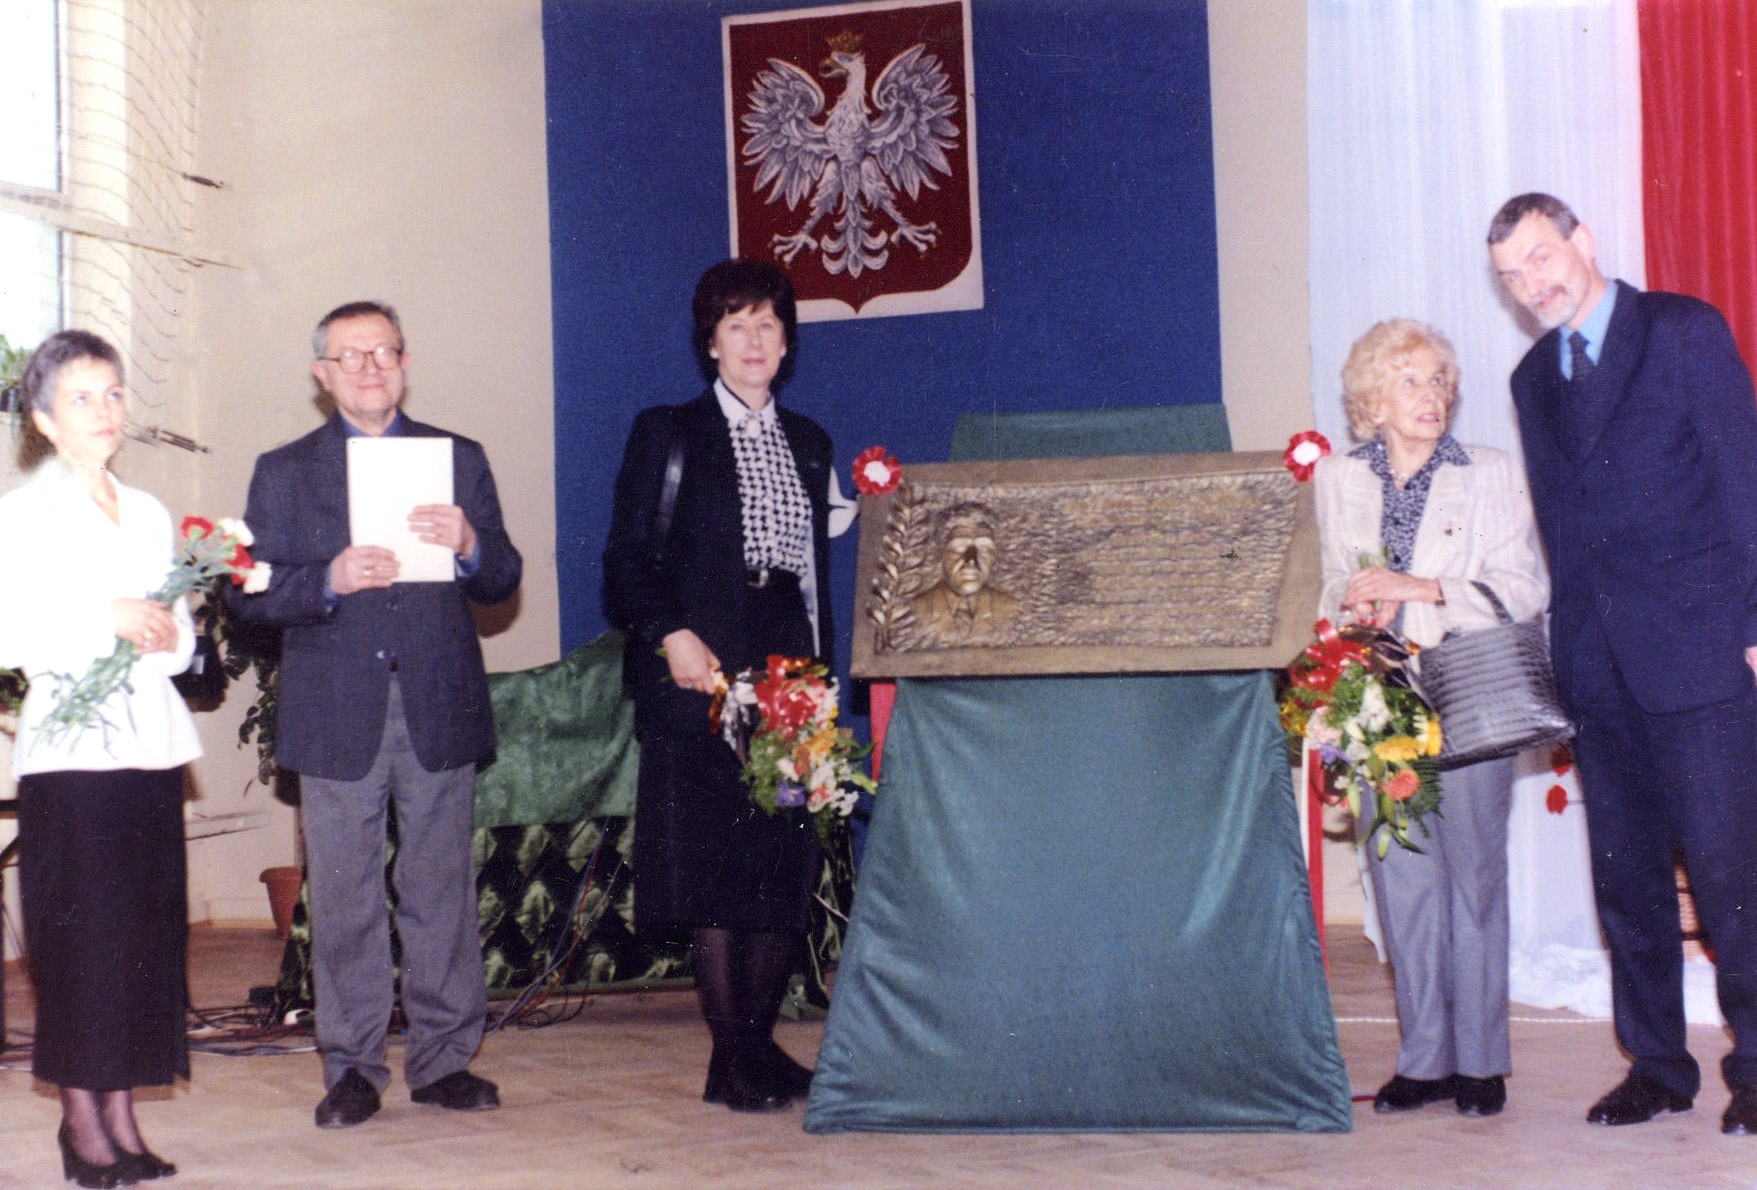
\includegraphics[width=0.6\textwidth]{photo/nadanie_imienia_szkole.jpg}
\caption[Nadanie imienia szkole]{Na zdj. od lewej: Marta Kluza, prof. Drozdowski, wnuczka Eugeniusza Kwiatkowskiego -- X. Puget, córka Eugeniusza Kwiatkowskiego i Czesław Świerczyński}
\end{center}
\end{figure}

Mało tego, gdy później znalazłem się bez pracy i nasza mama zaproponowała, że gotowa jest zrezygnować z połowy etatu, by mogła mnie zatrudnić na cały etat, ta owszem zgodziła się mnie zatrudnić, ale na ćwierć etatu. \textbf{To się nazywa czarna niewdzięczność!} Po pięciu latach w konkursie na dyrektora uzyskała tylko jeden głos na dziesięć możliwych! Wygrał Eugeniusz Bugaj...

W 2000 – jubileuszowym roku Elżbieta i Mirosław Głąbowie przepisali nam notarialnie działkę 295 a i b, a w październiku tego roku już potężna koparka zrobiła wykop pod fundamenty, tak że Henryk Gryl ze swym pomocnikiem przystąpili do drutowania ławy, na którą beton przywiózł już św. pamięci Antek Surowiec. Do 15 grudnia wybudowali całe piwnice i schody wejściowe. W 2001 r. zalali oba stropy i zakończyli murowanie domu, a Eugeniusz Starczewski położył dachówkę. W 2000 roku rozpoczęliśmy też walkę o przejęcie władzy w Spółdzielni Mieszkaniowej, którą zakończyliśmy sukcesem w 2001 r., wybierając nowe władze, w wyniku czego zostałem wiceprezesem Myszkowskiej Spółdzielni Mieszkaniowej. Nasza Mama na wszystkie świętości błagała mnie, bym tam nie szedł, bo tam mnie wykończą. Kto mógł jednak wtedy pomyśleć, że sądy są do tego stopnia przekupne!

Oto w maju 2001 r. poprzez rozmowy z członkami Myszkowskiej Spółdzielni Mieszkaniowej doprowadziliśmy do tego, że w poszczególnych osiedlach zostały wybrane na członków Walnego Zgromadzenia Mieszkańców osoby przeciwne dotychczasowej Radzie Nadzorczej i Zarządowi. Wyniki tajnych wyborów były liczone w obecności wyborców, co odbierało przegranym możliwość podważenia uczciwości tych wyborów. Przyznał to również  protokół polustracyjny, że nie było żadnych uchybień w postępowaniu komisji skrutacyjnych we wszystkich wyborach do Walnego Zgromadzenia oraz do Rady Nadzorczej. Mimo to najpierw Sąd Rejestrowy w Częstochowie nie wpisał nowego Zarządu do Rejestru, a następnie Sąd Okręgowy w Częstochowie wydał wyrok uznający roszczenia poprzedniej Rady Nadzorczej i nie odwołujący naszej Rady Nadzorczej, przy czym ów Sąd nie powiadomił nas o terminie rozprawy, na której został ów wyrok ogłoszony. W tej sytuacji wyrok absolutnie bezprawny uprawomocnił się, gdyż strona pozwana, tzn. nasza Rada Nadzorcza i Zarząd nie wiedząc o wyroku nie odwołała się od niego we właściwym terminie!!! Natomiast stara Rada Nadzorcza, wiedząc, że będziemy sobie mogli przywrócić termin w związku z niepoinformowaniem nas, tj. pozwanego o rozprawie i o zapadłym nań wyroku, najęła sobie pseudoochroniarzy bez uprawnień i zajęła z pomocą pracowników MSM budynek Spółdzielni! Jednym słowem oszuści najęli sobie chuliganów do bezprawnego przejęcia własności, do której nie mieli tytułu prawnego!

Owo siłowe przejmowanie Spółdzielni filmował nasz pracownik, który od pół roku był na zwolnieniu lekarskim. Ja mu zakazałem mnie filmować i kilkakrotnie powtórzyłem mój sprzeciw, gdy jednak ów nie przerwał filmowania, wówczas podszedłem do niego i złapawszy obiektyw kamery skierowałem go w dół. Wówczas rzucili się na mnie ochroniarze, którzy wykręcili mi ręce do tyłu, dłońmi między łopatki i w takiej bolesnej pozycji mi je skuli. Dopiero po godzinie mnie rozkuli. Ów filmujący mnie pracownik złożył do Sądu Rejonowego Wydziału Karnego doniesienie o przestępstwie, że uderzyłem go w prawy policzek prawą dłonią, co z oczywistych względów jest niemożliwe. Sąd jednak, chcąc mnie skazać, nie tylko nie zarzucił oskarżycielowi oczywiste kłamstwo, ale rozszerzył akt oskarżenia o uderzenie oskarżyciela w policzek poprzez energiczne uchwycenie obiektywu kamery. Wszystko po to, by mnie pozbawić mandatu radnego, gdyż radnym nie może być osoba skazana prawomocnym wyrokiem. Dopiero Sąd okręgowy zmienił wyrok ze skazującego, ale koszty sądowe pozostały po mojej stronie.

Drogi mój Piotrusiu, prawniku z wielką lub marną przyszłością! Wielką, gdy czyjaś moc postanowi gruntownie, aż do fundamentów uzdrowić w państwie polskim wymiar sprawiedliwości, marną, jeśli będą nim rządzić szumowiny, takie jak w rządzie Donalda Tuska... Odwołał on Mariusza Kamińskiego, z funkcji prezesa Centralnego Biura Antykorupcyjnego za to, że ów przyłapał jego kolegów na korupcji!!! Jeśli takie rzeczy dzieją się na szczytach władzy, to co się może dziać w tzw. \textbf{,,Terenie''?!} Uczciwy prawnik to dla dzisiejszego establishmentu największe zagrożenie, więc tacy będą tępieni, jak tkanka rakowa tępi resztki zdrowego organizmu, mimo że jest jej żywicielem. Wielkie zadanie przed Tobą – Synu, wierzę, że mu podołasz choćby nawet z pomocą obcego mocarstwa, gdyż fundamentem państwa jest uczciwy wymiar sprawiedliwości... Cóż nam po suwerenności naszego państwa, kiedy w nim obywatel żyje w jarzmie niesprawiedliwego prawa i niesprawiedliwych sądów i urzędów!

Na trzy dni przed ową napaścią na prawowity Zarząd i Radę Nadzorczą MSM zostałem odwołany przez Radę Nadzorczą kierowaną przez pana Kluzę z funkcji wiceprezesa Spółdzielni. Moje miejsce zajął dotychczasowy prezes Augustynowicz – marny, mały człowieczek, ale bardzo elokwentny, na którego nasi przeciwnicy mieli haka, więc wił się jak piskorz pomiędzy wymaganiami Rady Nadzorczej, a żądaniami jego szantażystów. Natomiast prezesem został pan Kluza, który teraz dopiero poczuł się pewien na tym stanowisku! Zwykła kanalia, pijak, na którego mieli wiele haków, intrygant. Gdy w ogniu walki trzeba było okazać się odwagą podpisał rezygnację ze stanowiska prezesa, co spowodowało dodatkowe zamieszanie, które było bardzo na rękę oszukańczym uzurpatorom władzy nad Spółdzielnią.

Opatrzność jednak nade mną nadal czuwała, tylko ja Jej nie słuchałem z należytą pilnością! Szatan bowiem robił wszystko, bym nie wrócił do szkolnictwa, a nawet gdybym tam trafił, to na bardzo krótko. Musiałem mu dobrze zajść za skórę, skoro mnie tyle razy usiłował odsunąć od katedry... Pierwszy raz w związku z konfliktem z dyr. Tarłowskim wylądowałem w Hucie „Katowice”, drugi raz znękany utyskiwaniem Mamy na niskie zarobki wylądowałem w Kopalni „Boże Dary”, trzeci raz z powodu konfliktu z Martą Kluzą, która wymierzyła mi absolutnie nieuzasadnioną karę nagany (takie było jej podziękowanie za to, że jej załatwiłem stanowisko dyrektora) oraz złożoną mi propozycją pełnienia funkcji wiceprezesa Spółdzielni Mieszkaniowej! Czwarty raz był wówczas, gdy w lutym 2003 r. nie zgłosiłem swego udziału w konkursie na dyrektora Szkoły Podstawowej i Gimnazjum w Mrzygłodzie, a jak się później okazało miałem absolutne szanse jego wygrania, bowiem niemal wszystkich członków komisji konkursowej miałbym za sobą. \textbf{To był jeden z moich najcięższych błędów w życiu!}

\textbf{25 października 2002 r., w piątek zmarła moja mama, a Wasza babcia Radegunda na zawał serca w Zabrskim Szpitalu.} W październiku też powiększyłem szeregi bezrobotnych. 27 października odbyły się wybory do Rady Miasta, a 28, w dniu pogrzebu Babci dowiedziałem się, że zostałem radnym na drugą kadencję.
\begin{figure}[!h]
\begin{center}
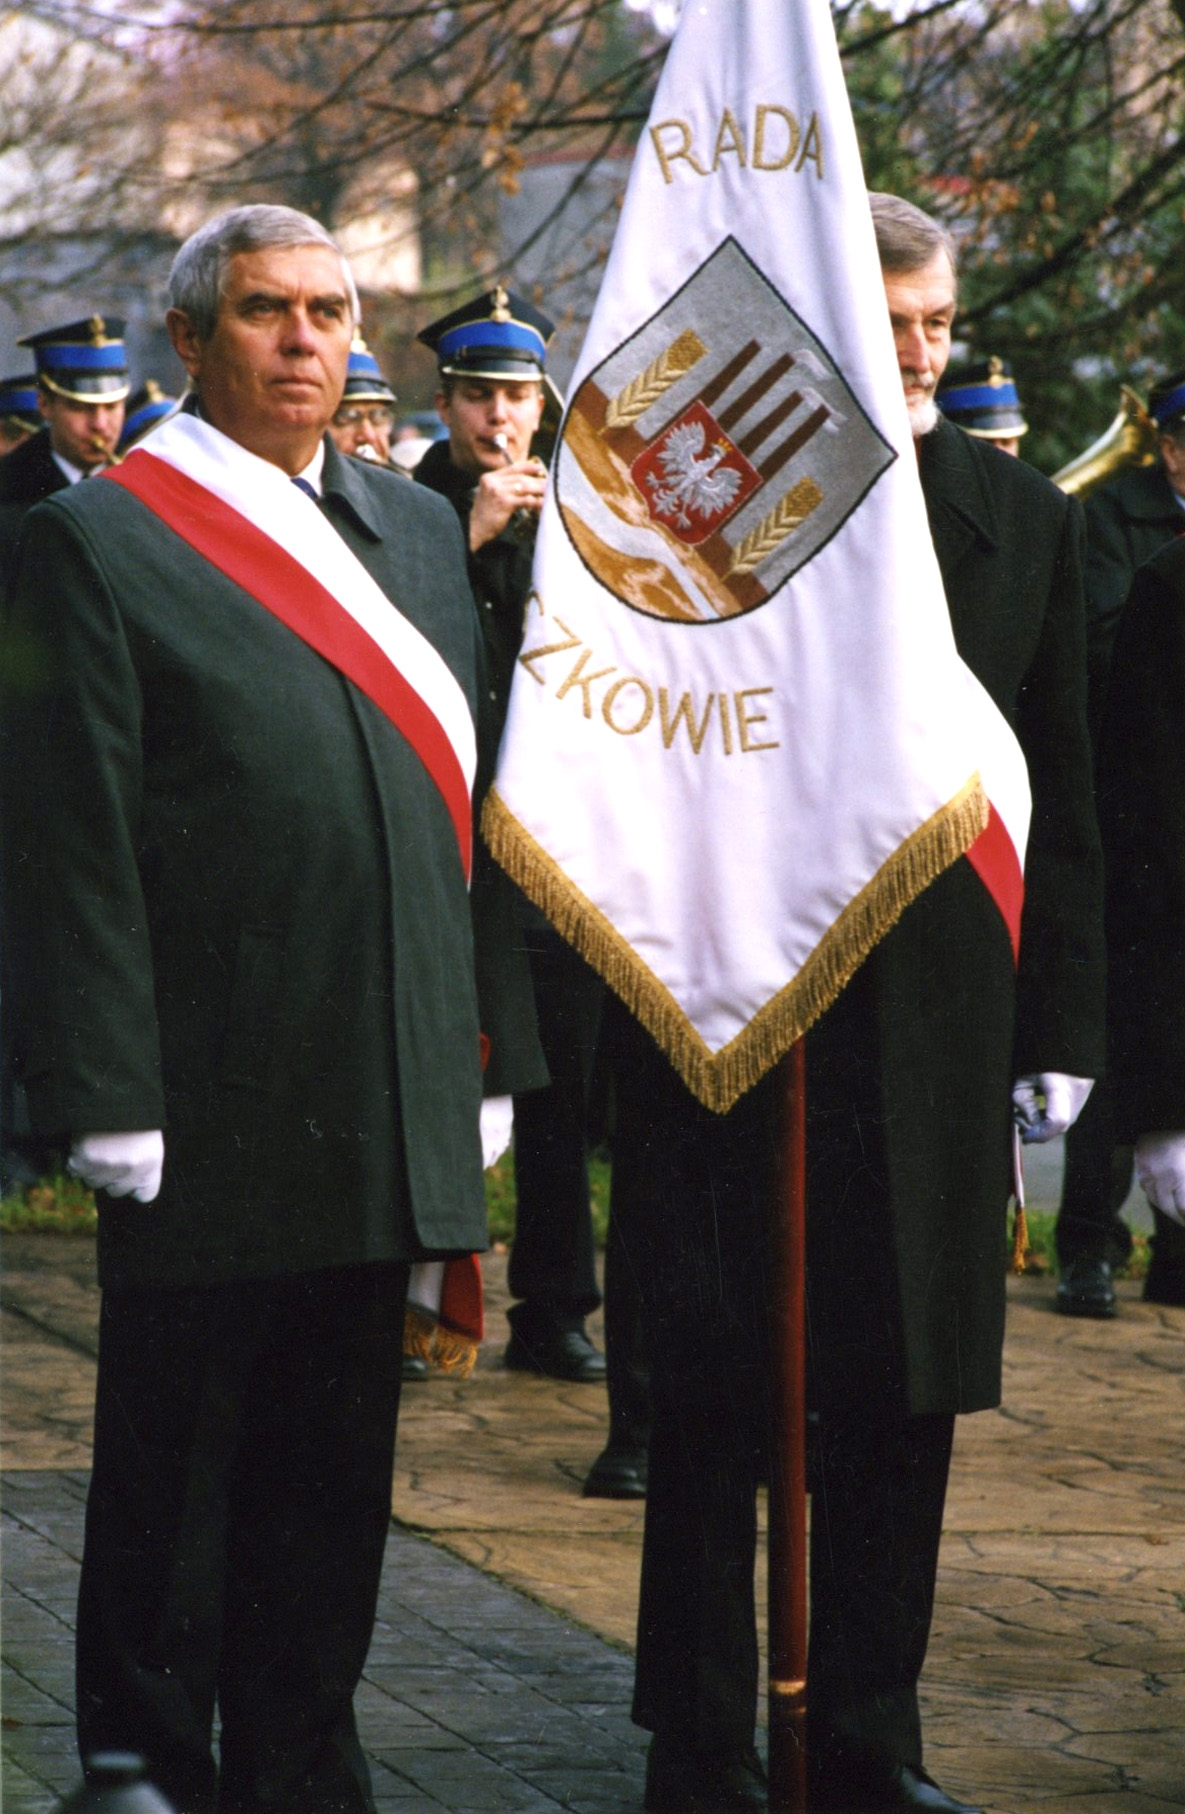
\includegraphics[width=0.3\textwidth]{photo/czeslaw_swierczynski_ze_sztandarem_rady_miasta.jpg}
\caption[Poczet sztandarowy]{Na zdj.: Włodzimierz Pasek i Czesław Świerczyński ze sztandarem Rady Miasta Myszkowa.}
\end{center}
\end{figure}

Mimo że wybory wygrał „nasz” człowiek – Leon Okraska, ja pozostawałem bez pracy. Dopiero 17 marca 2004 r. zostałem zatrudniony na stanowisku terapeuty w Środowiskowym Domu Samopomocy przy ul. Gałczyńskiego, gdzie pracowałem do 13 sierpnia tego roku w ramach tzw. prac interwencyjnych. Od 1 września zostałem zatrudniony w ZSP Nr 3 w Myszkowie w świetlicy i jako nauczyciel języka polskiego w klasie czwartej. Wówczas to zobaczyłem po latach jak bardzo rozbisurmanione są dzieci, niezdolne do żadnej uwagi i wyzbyte jakiegokolwiek szacunku dla nauczyciela i dorosłych. I gdy próbowałem doprowadzić niektórych z nich do porządku, uderzając ich książką w miękkich okładkach po głowie, burmistrz Okraska zrobił z tego aferę, że biję dzieci, by mnie zwolnić dyscyplinarnie ze szkoły, bez prawa uprawiania zawodu nauczycielskiego! Dopiero najbliższe otoczenie (Bogdan Cygankiewicz i Andrzej Hutnik) zmyło mu głowę na tyle, że zaniechał mnie. Do czego to prowadzi, że nawet za najlżejsze karanie cielesne dzieci nauczyciel może stracić pracę, a dziecka dopuszczającego się daleko gorszych czynów wobec nauczyciela nie można ze szkoły wydalić bez zgody rodziców! Uważam, że jest to świadoma dywersja wobec naszego systemu wychowania, a w konsekwencji wobec naszego narodu, bowiem takie będą Rzeczypospolite, jakie ich dzieci chowanie!

W czerwcu 2004 r. Marta Kluza sromotnie przegrała konkurs na dyrektora Zespołu Szkół Nr 1, więc była skłonna przyjąć mnie do pracy na etat polonisty i katechety. Warunkiem było uzyskanie od Arcybiskupa misji kanonicznej do nauczania religii katolickiej... I mi jej ksiądz arcybiskup Stanisław Nowak odmówił, podczas gdy w tej szkole było wolnych godzin katechezy na cały etat, a katechizowała tam w sposób urągający dydaktyce m.in. Małgorzata Janocha  siostra księdza pełniącego funkcję kapelana przy tym arcybiskupie. Pewnie go Jezus Chrystus na Sądzie Ostatecznym zapyta o to moje niedoszłe katechizowanie w Zespole Szkół Nr 1 w Myszkowie!  Dzięki ustępstwu dyr. Anity Marek mogłem 1 października 2004 roku przejść na wcześniejszą emeryturę, z czego w tej sytuacji skwapliwie skorzystałem...

W marcu 2007 r. objąłem dzięki Jadwidze Wiśniewskiej – poseł na Sejm RP z ramienia Prawa i Sprawiedliwości - stanowisko komendanta Ochotniczego Hufca Pracy w Myszkowie z siedzibą na Helenówce. Dość szybko się zorientowałem, że jest to instytucja powielająca funkcje wychowawcze wychowawców Zespołu Szkół (Zawodowych) Nr 1 w Myszkowie. Funkcje wychowawcze dość rzetelnie wykonywał jedynie Artur Rynkiewicz. Pozostali wychowawcy okazali się zwykłymi obibokami. Jednak niektórzy z nich skwapliwie pisali sprawozdania z fikcyjnych akcji wychowawczych realizowanych wg wydumanego programu wychowawczego. Jednym słowem wielka mistyfikacja! Co robić?! Czy kontynuować ją, czy też uciąć tę gałąź, na której się siedzi, upaść boleśnie i spowodować utratę pracy przez moich podwładnych – prywatnie utrzymujących z pracy w OHP swe rodziny? Postanowiłem założyć Gimnazjum dla Dorosłych, lecz zamiast rzecz prywatnie przeprowadzić, zaangażowałem w to dzieło Zakład Doskonalenia Zawodowego. Wszystko byłoby się pomyślnie zakończyło, gdyby nie upadek rządu Jarosława Kaczyńskiego w 2007r.

W związku z XX rocznicą pierwszych częściowo wolnych wyborów z 4 czerwca 1989 r. miałem dzięki poseł Jadwigi Wiśniewskiej honor uczestniczyć w tych uroczystościach w Pałacu Prezydenckim.
\begin{figure}[!h]
\begin{center}
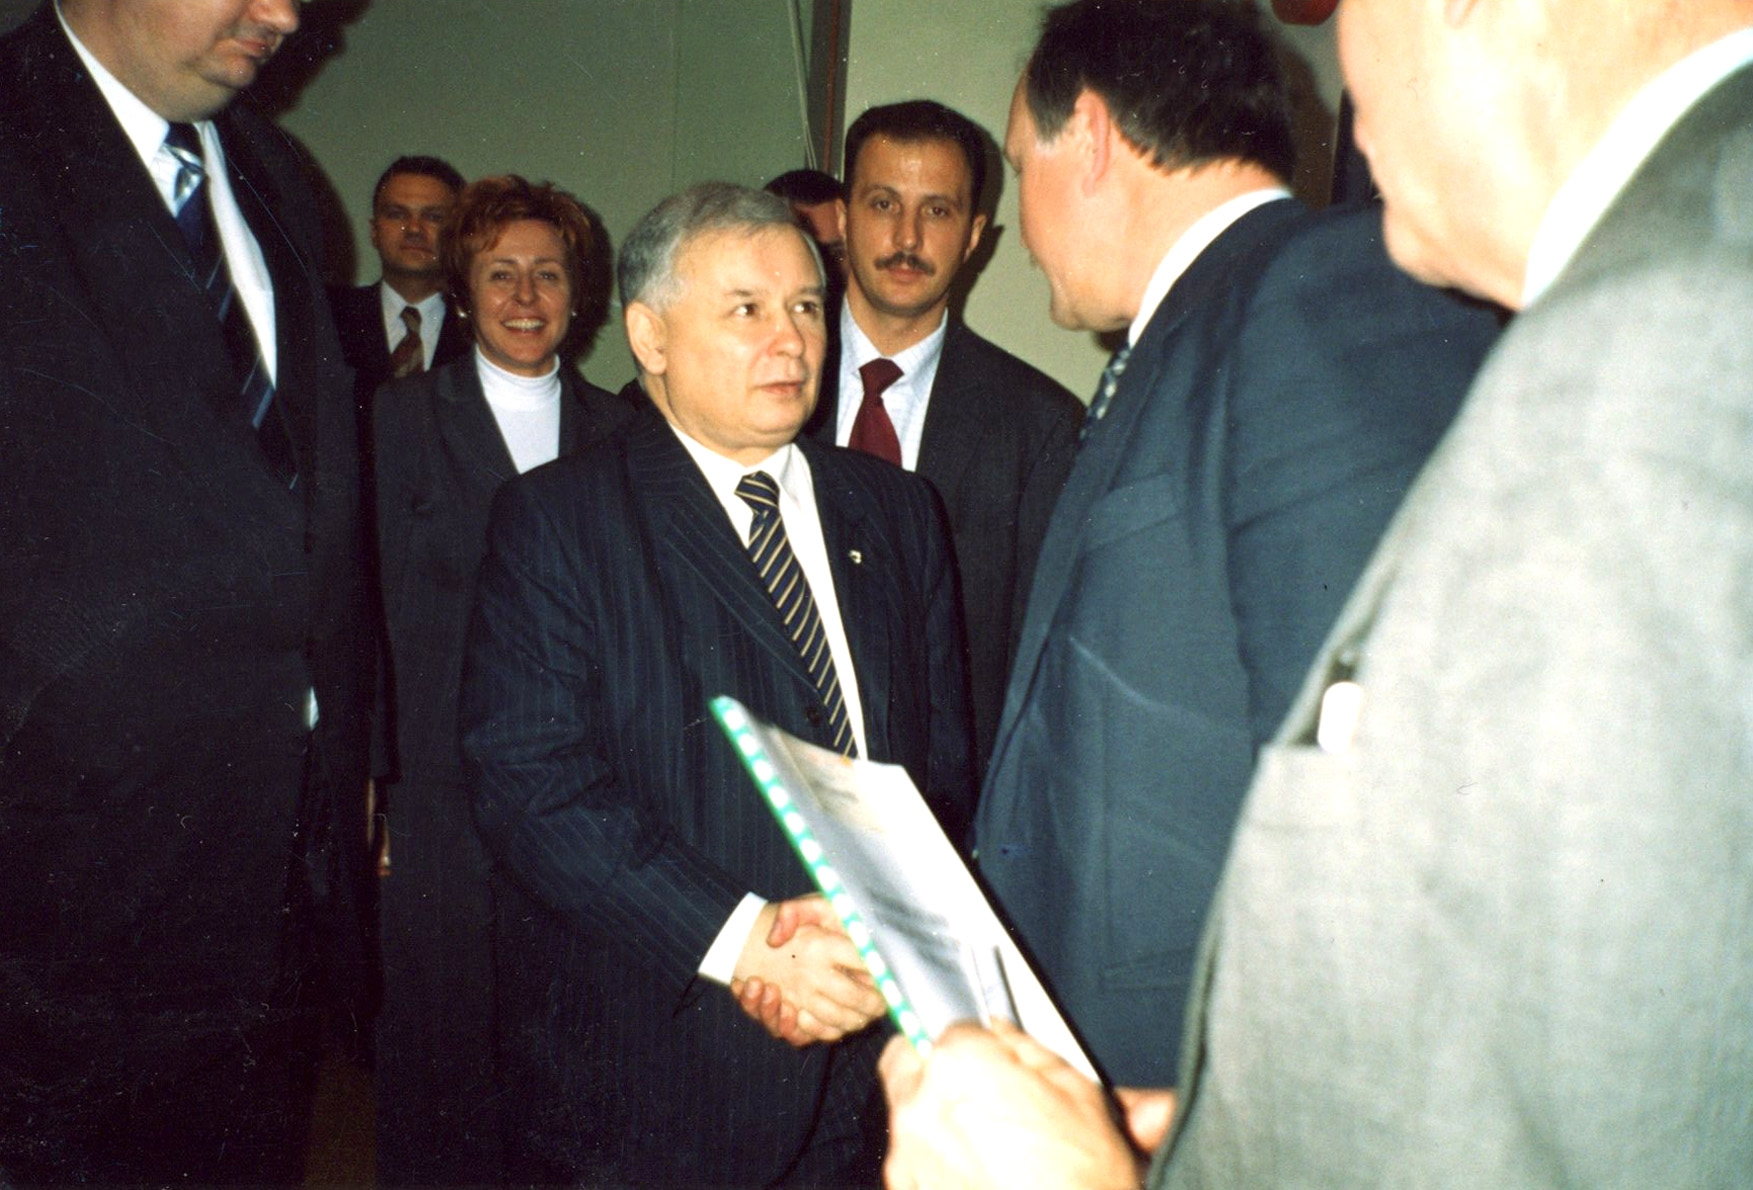
\includegraphics[width=0.7\textwidth]{photo/jaroslaw_kaczynski.jpg}
\caption[Jadwiga Wiśniewska]{N zdj. w głębi poseł Jadwiga Wiśniewska, na pierwszym planie Jarosław Kaczyński.}
\end{center}
\end{figure}

Pierwszy i ostatni raz widziałem tak blisko Prezydenta Lecha Kaczyńskiego. Potem, w 2010 r. były uroczystości pogrzebowe Lecha i Marii Kaczyńskich - pary Prezydenckiej w Krakowie, którzy zginęli w zamachu w Smoleńsku wraz z 94 osobami pełniącymi najważniejsze funkcje w RP. Za jednym zamachem Putin wraz z Tuskiem i jego zgrają pozbawili nasze Państwo i naród głowy, tj. ludzi prawdziwie zatroskanych o losy naszej Ojczyzny, o jej suwerenność!!! Również dzięki poseł Jadwigi Wiśniewskiej otrzymałem VIP-owską kartę wstępu na uroczystość beatyfikacji ks. Jerzego Popiełuszki, która odbyła się 6 czerwca w Warszawie. Byłem wśród wielu kolegów z czasu internowania i co najważniejsze - blisko ołtarza.
\begin{figure}[!h]
\begin{center}

\includegraphics[width=0.5\textwidth]{photo/beatyfikacja_popieluszki_karta_wstepu.jpg}
\caption[Karta vipowska]{Beatyfikacja błog. Jerzego Popiełuszki -- vipowska karta wstępu}
\end{center}
\end{figure}

Od września 2009 r. trwały przygotowania do uroczystości katyńskich, których kulminacja miała nastąpić w kwietniu i maju 2010 r. w 70. rocznicę  sowieckiego mordu na oficerach polskich w Katyniu, Miednoje i Charkowie. Ja wraz z kilkoma polonistami i historykami byłem zaangażowany w pracach jury konkursu katyńskiego. Za to moje zaangażowanie otrzymałem możliwość bezpłatnego uczestnictwa w wycieczce do Nowogródka, Zaosia, Kuropat, Smoleńska, Katynia, Powiewiórek, Ponar oraz Wilna wraz z laureatami tego konkursu oraz pracownikami IPN-u, co czyniło z tej wycieczki wspaniały wykład historyczny maksymalnie upoglądowiony.
\begin{figure}[!h]
\begin{center}
\includegraphics[width=0.6\textwidth]{photo/czeslaw_swierczynski_w_kontuszu_w_zaosiu.jpg}
\caption[Czesław Świerczyński w kontuszu]{Czesław Świerczyński w kontuszu w dworku Mickiewiczów w Zaosiu}
\end{center}
\end{figure}

Szczęśliwie usiadłem obok księdza dra Jacka Plecha, duszpasterza akademickiego z Katowic, dzięki czemu dostąpiłem łaski służenia we wszystkich Mszach świętych w tych niezwykłych miejscach, bliskich sercu każdego Polaka patrioty: w Nowogródku, w Katyniu, w Smoleńsku, w Kuropatach, w Ostrej Bramie.
\begin{figure}[!h]
\begin{center}
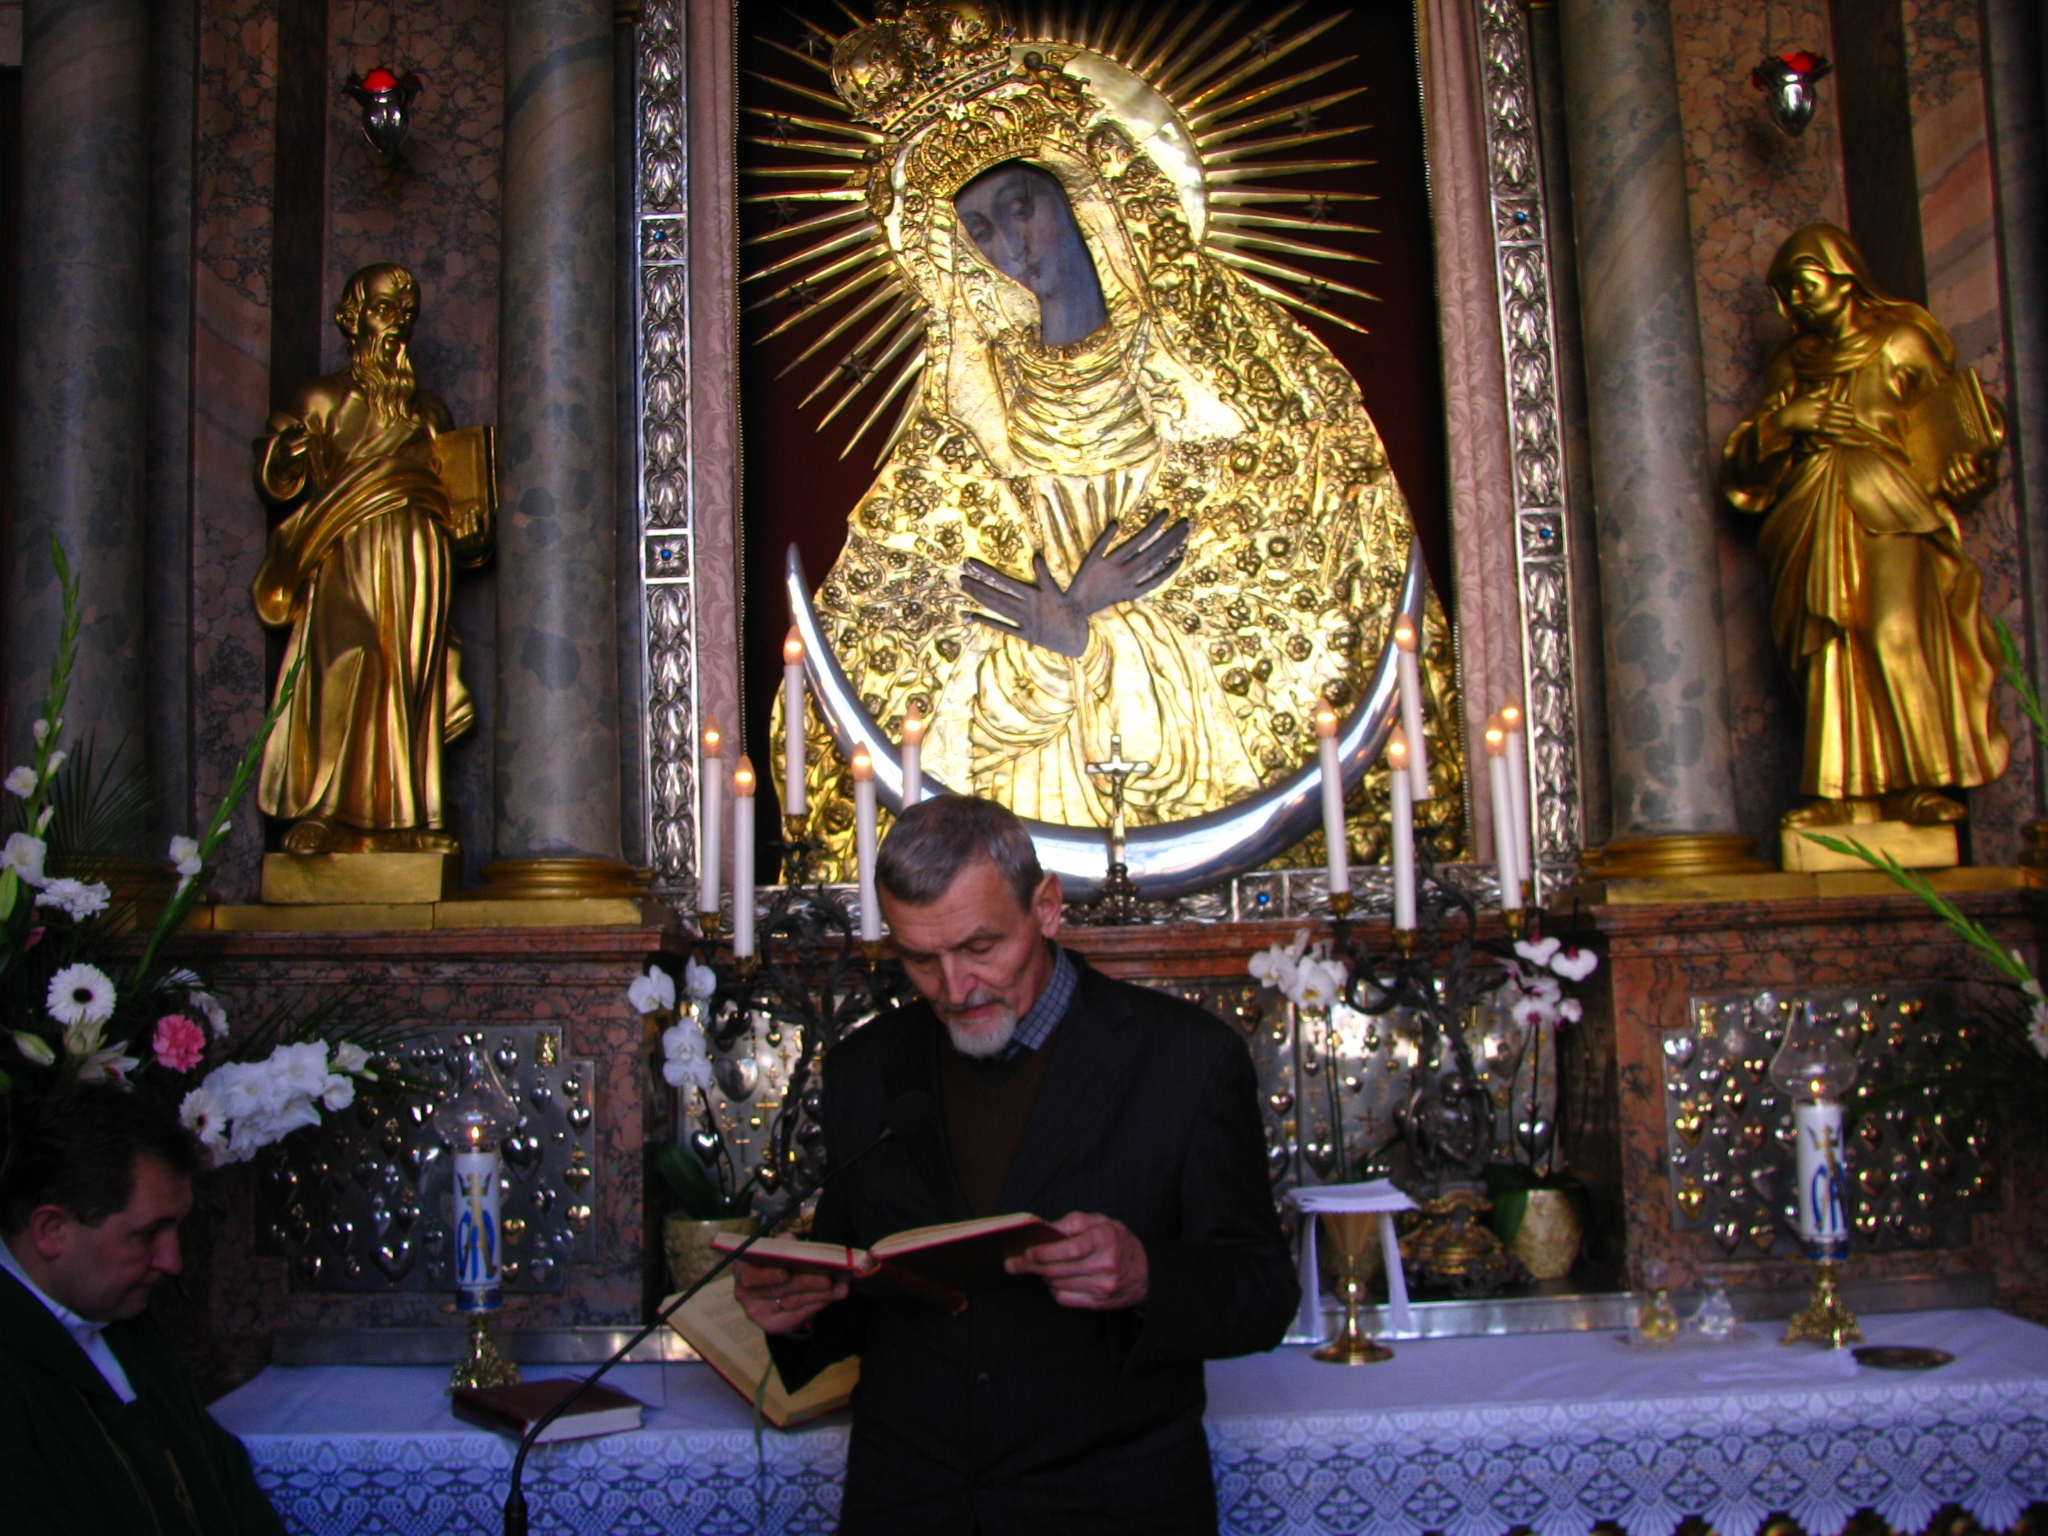
\includegraphics[width=0.7\textwidth]{photo/czeslaw_swierczynski_ostra_brama.jpg}
\caption[Ostra Brama]{Na zdj. Czesław Świerczyński czyta lekcję przed obrazem Matki Bożej Ostrobramskiej.}
\end{center}
\end{figure}

Nie przyszło mi do głowy, że za kilka miesięcy będę na wniosek prokuratury rosyjskiej przesłuchiwany przez Polską Prokuraturę Wojskową na okoliczność ewentualnego zabrania z miejsca katastrofy prezydenckiego samolotu jakichś jego szczątków. Na złodzieju czapka gore! Putin się boi, że na podstawie tych szczątków, które workami stamtąd wywozili różni ludzie, więc mogły trafić one np. w jedno miejsce, gdzieś do laboratorium w Zachodniej Europie albo USA, z tak wielu szczątków można przy dzisiejszej technice określić przyczyny katastrofy, które Rosjanie znają, gdyż wraz z naszymi łajdakami ją spowodowali, tj. wybuch bomby termobarycznej na pokładzie prezydenckiego tupolewa. Ciekawe gdzie tę bombę zainstalowano? W Samarze czy w Warszawie, tuż przed jego drugim lotem do Smoleńska?
\begin{figure}[!h]
\begin{center}
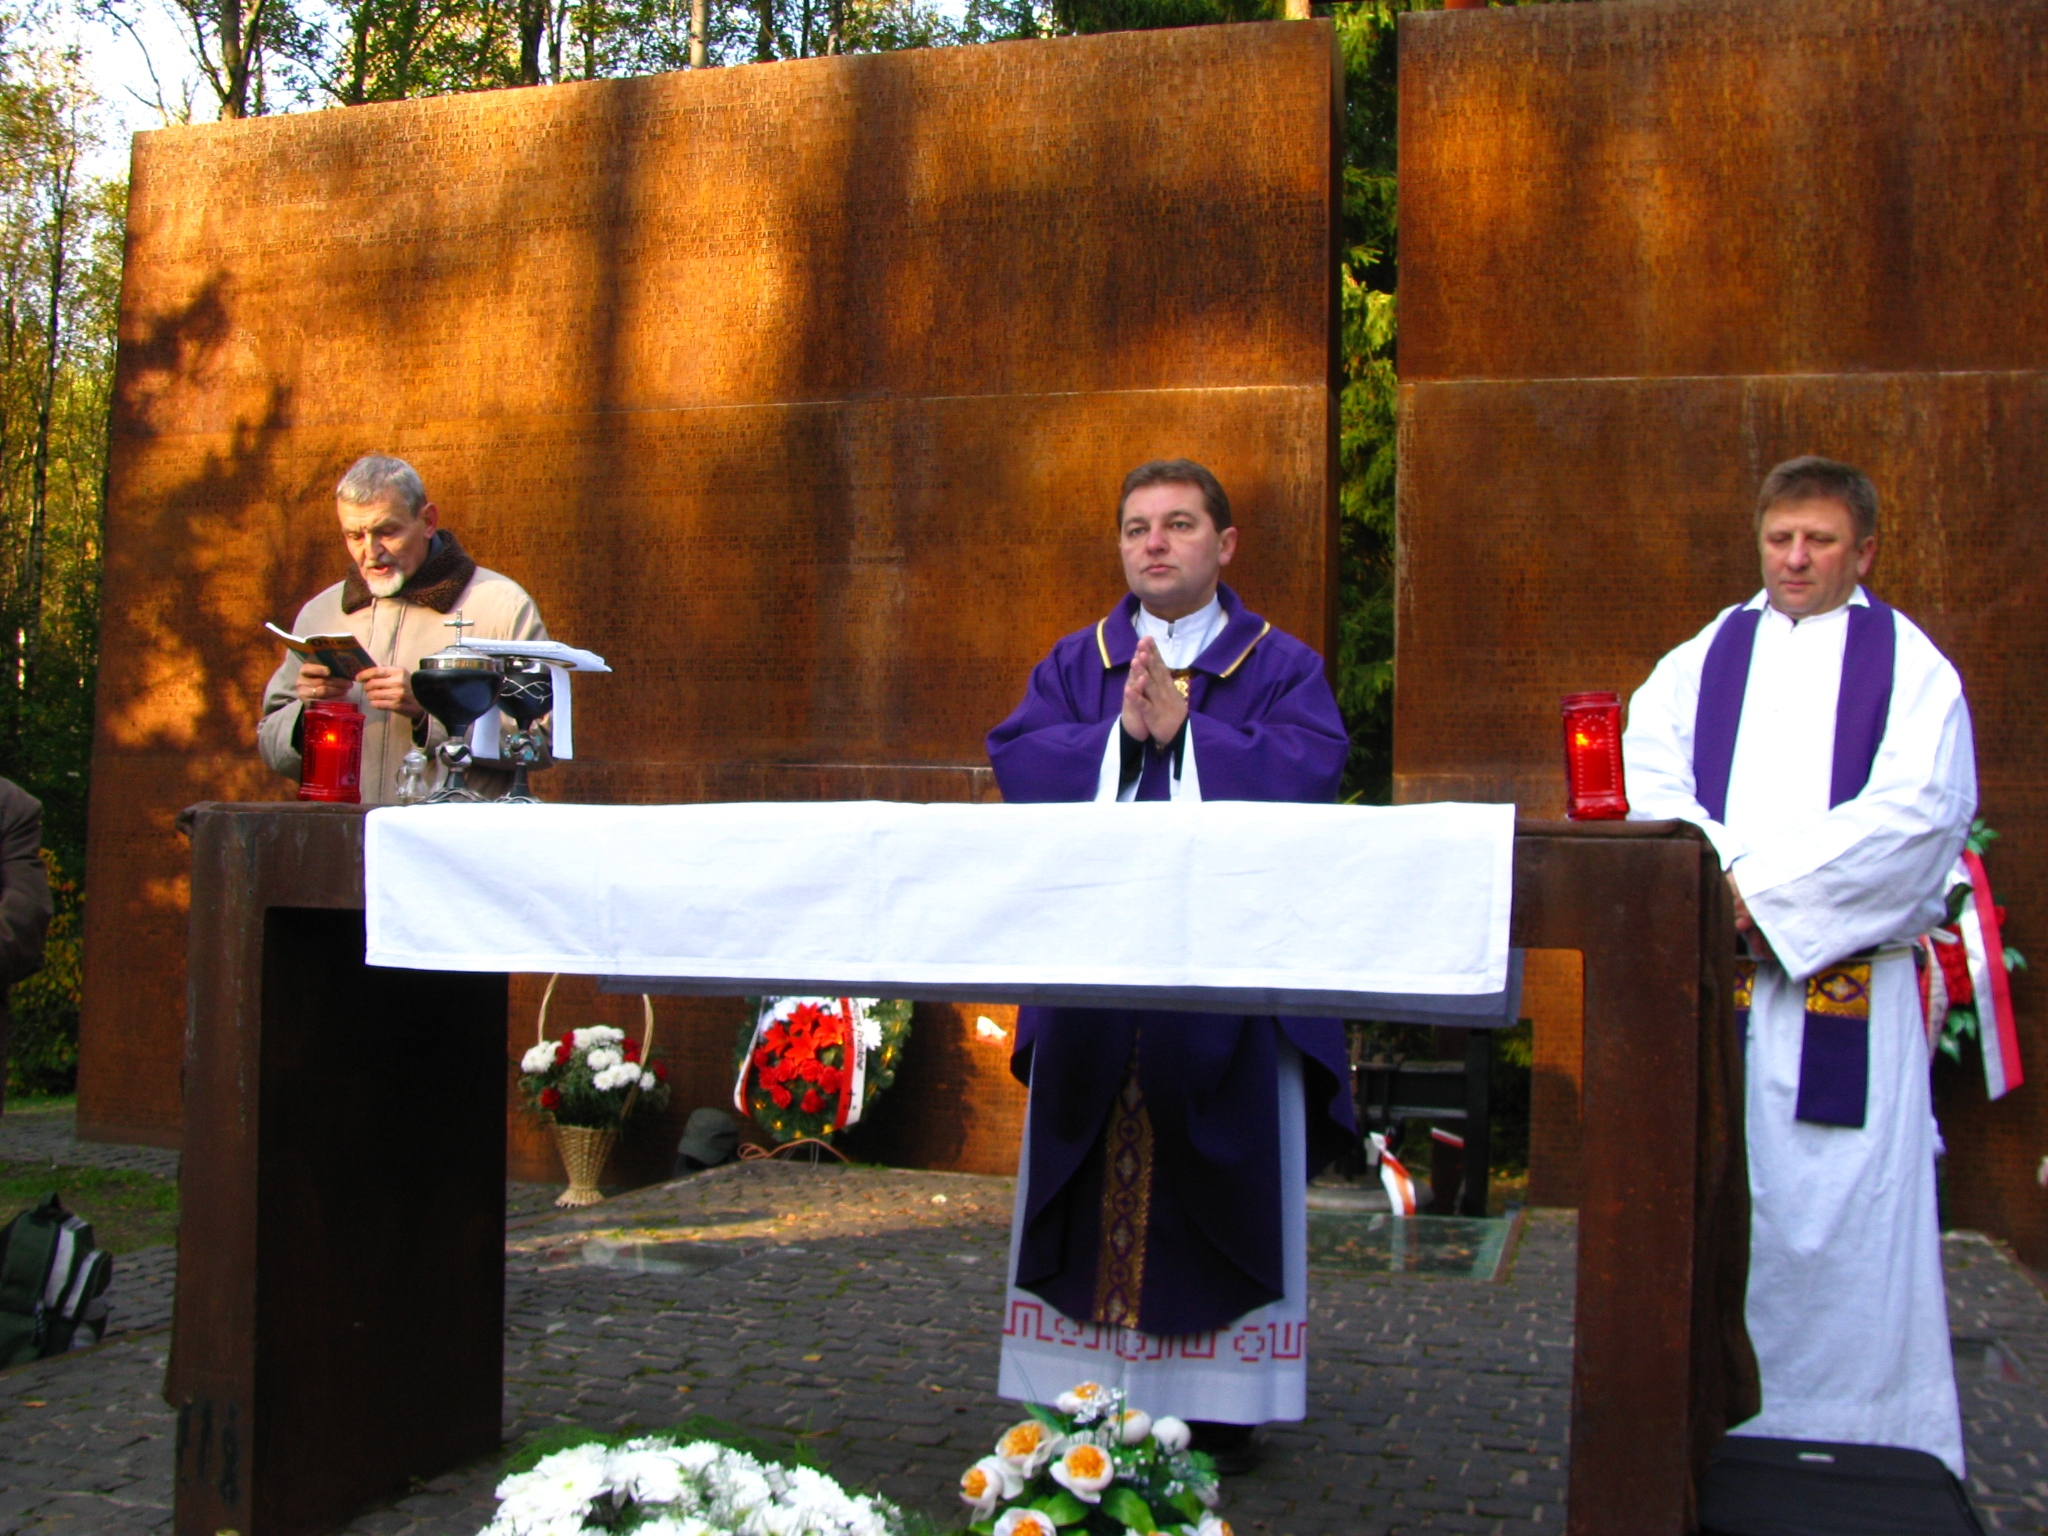
\includegraphics[width=0.6\textwidth]{photo/czeslaw_swierczynski_katyn_1.jpg}
\caption[Katyń]{Na zdj. Czesław Świerczyński czyta lekcję, msze św. odprawia ks. Jacek Plech.}
\end{center}
\end{figure}

Pewnie Tusk nie zgodziłby się na lot z taką bombą. Po co jednak przesłuchują nas – uczestników wycieczki do Smoleńska? Po to, by wykluczyć medialnie możliwość wywiezienia szczątków prezydenckiego tupolewa z Rosji, bo któż się przyzna Ruskim, że wywiózł? A Rosjanie będą mieli alibi, że wszystkie szczątki, na jakich przeprowadzono badania w polskich czy zachodnich laboratoriach nie pochodzą z samolotu, który uległ katastrofie w Smoleńsku! Ja na przesłuchaniu udałem zdziwienie, jakże oni mogą jeszcze w pięć miesięcy po oświadczeniu minister Kopacz, że niby Rosjanie w maju 2010 r. przekopali na głębokość 1,5 m miejsce katastrofy i przesiali całą tę ziemię, oczekiwać, że po tym przkopaniu i przesianiu ktokolwiek tam jeszcze mógł coś znaleźć. A na pytanie czy wiem o wywiezionych stamtąd szczątkach samolotu, odpowiedziałem, że owszem wiem, bo rozpisywały się o tym liczne czasopisma oraz pokazywała to telewizja. Tak oto katastrofa smoleńska, czyli ruski zamach na Polskiego Prezydenta dotknęła również waszego ojca - Moje Drogie Dzieci.








\clearpage
\section{Moje dzieci}

Najstarsze nasze dziecię to śliczna \textbf{Zuzia}, która przyszła na świat \textbf{18 lutego 1975 r. w szpitalu w Katowicach Bogucicach} prosto w ręce babki Lehmanki. I bardzo dobrze, gdyż poród był pośladkowy, więc gdyby się Zuziczek rodził w Myszkowie niechybnie nabawiliby ją tamtejsi lekarze partacze zwichnięcia stawu biodrowego... Miała być, zgodnie z moimi oczekiwaniami – chłopcem, dlatego nazywałem Ją Zuzikiem. Na kilka dni przed rozwiązaniem wujek Mirek wymógł na mnie, bym wyszukał jakieś imię dla dziewczynki i znalazłem Zuzannę, bo mi się jego brzmienie podobało. Gdy mi stryjenka Irena przez telefon z entuzjazmem gratulowała córki, myślałem, że sobie kpi ze mnie. Ta moja złość na zrządzenie losu (wówczas bowiem byłem ateistą) trwała do momentu, gdy moja maleńka córunia spojrzała na mnie swoimi, wówczas błękitnymi oczętami, tak że się w niej zakochałem, co mi zostało do dzisiaj.

\begin{figure}[!h]
\begin{center}
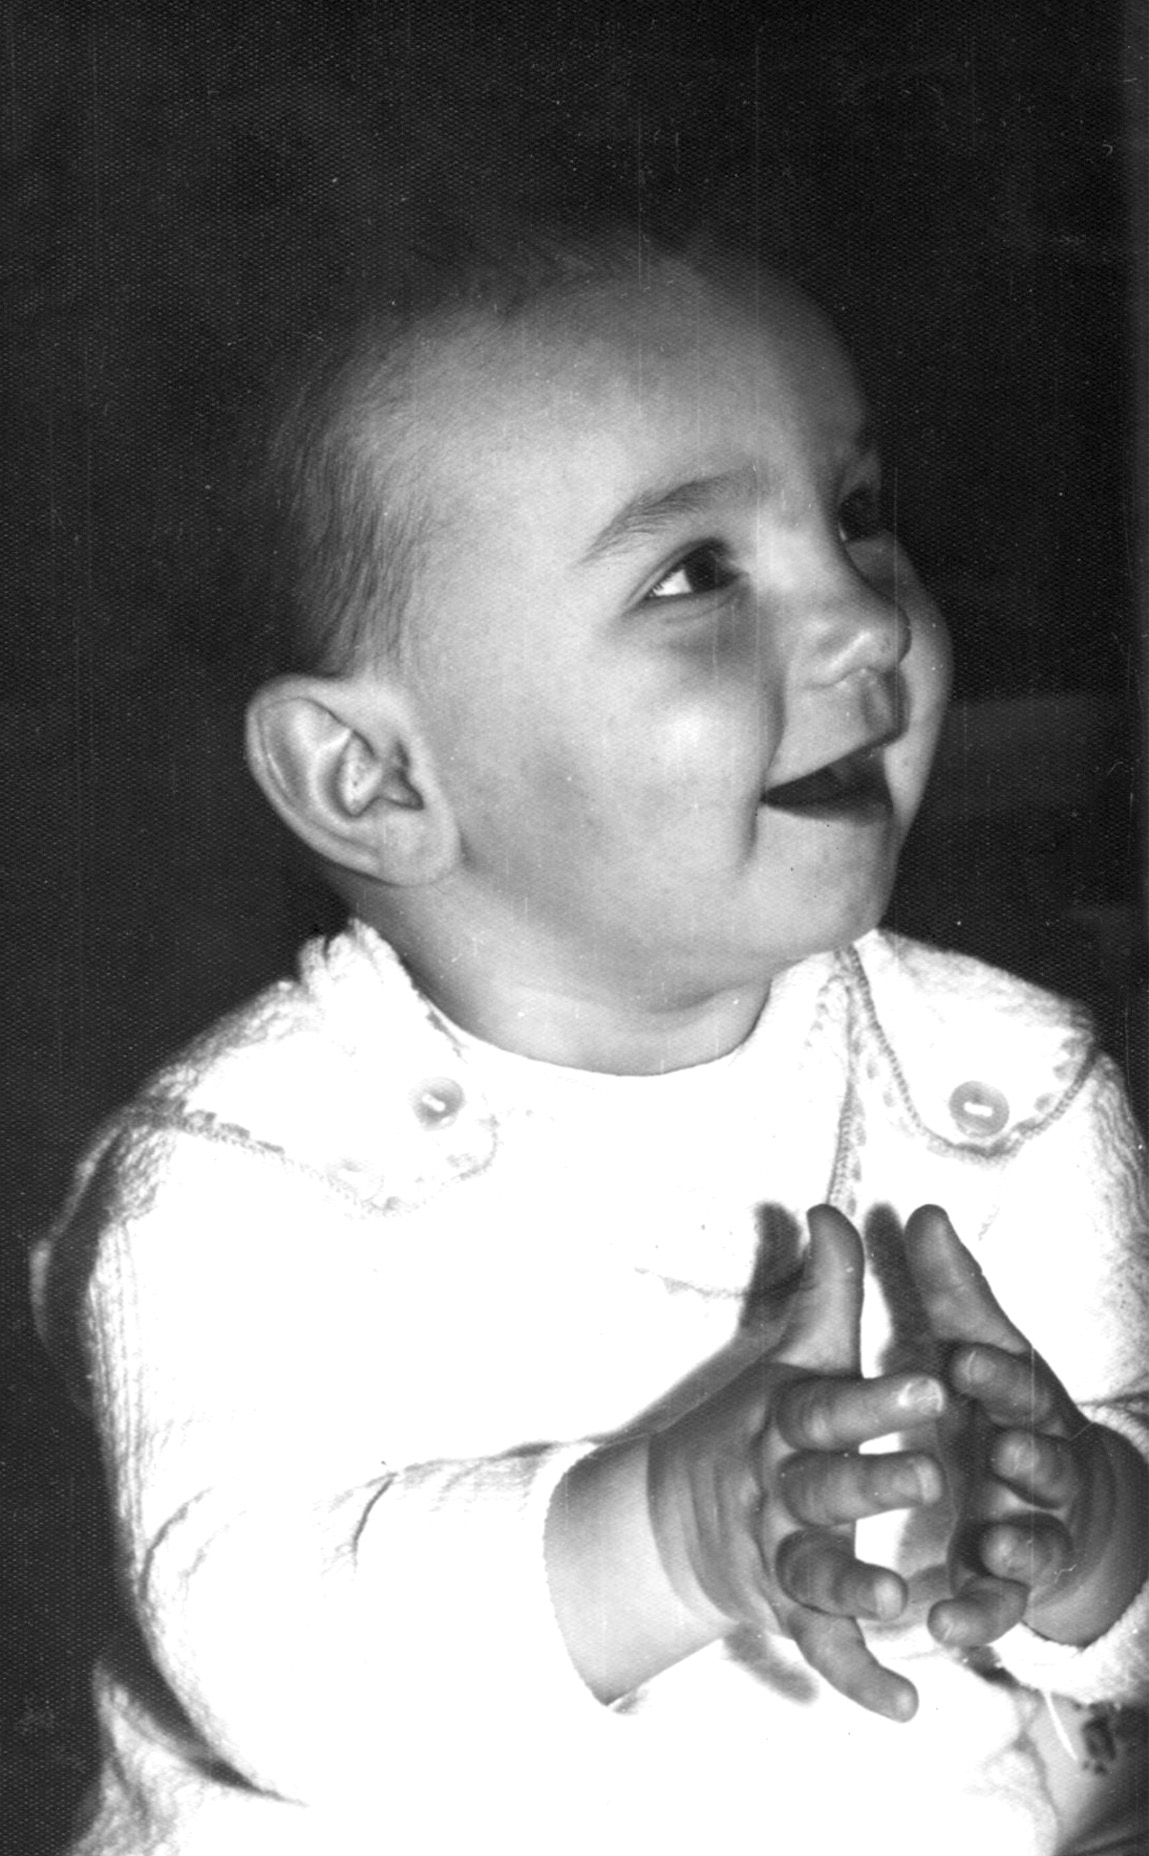
\includegraphics[width=0.3\textwidth]{photo/zuzia_swierczynska_2.jpg}
\caption{Roczna Zuzia Świerczyńska}
\end{center}
\end{figure}

Zuzik jakby się przejął tym moim oczekiwaniem, że miała być chłopakiem i rej wodziła dzieciom mirowskim, a gdy jako trzylatek znalazła się w Myszkowie, nie chciała wejść do bloku, jakby czuła, że się kończy jej piękna przygoda z Mirowem... Swoim mirowskim zwyczajem przyłączyła się do grupki chłopców, którzy jednak nie chcieli z nią chadzać. Wkrótce też poskarżył nam się Zuzik, że ją chłopcy przezywają „dziewcyna”. Niedługo ta pretensja minęła, gdy poszła do Przedszkola Nr 4 na górce.
\begin{figure}[!h]
\begin{center}
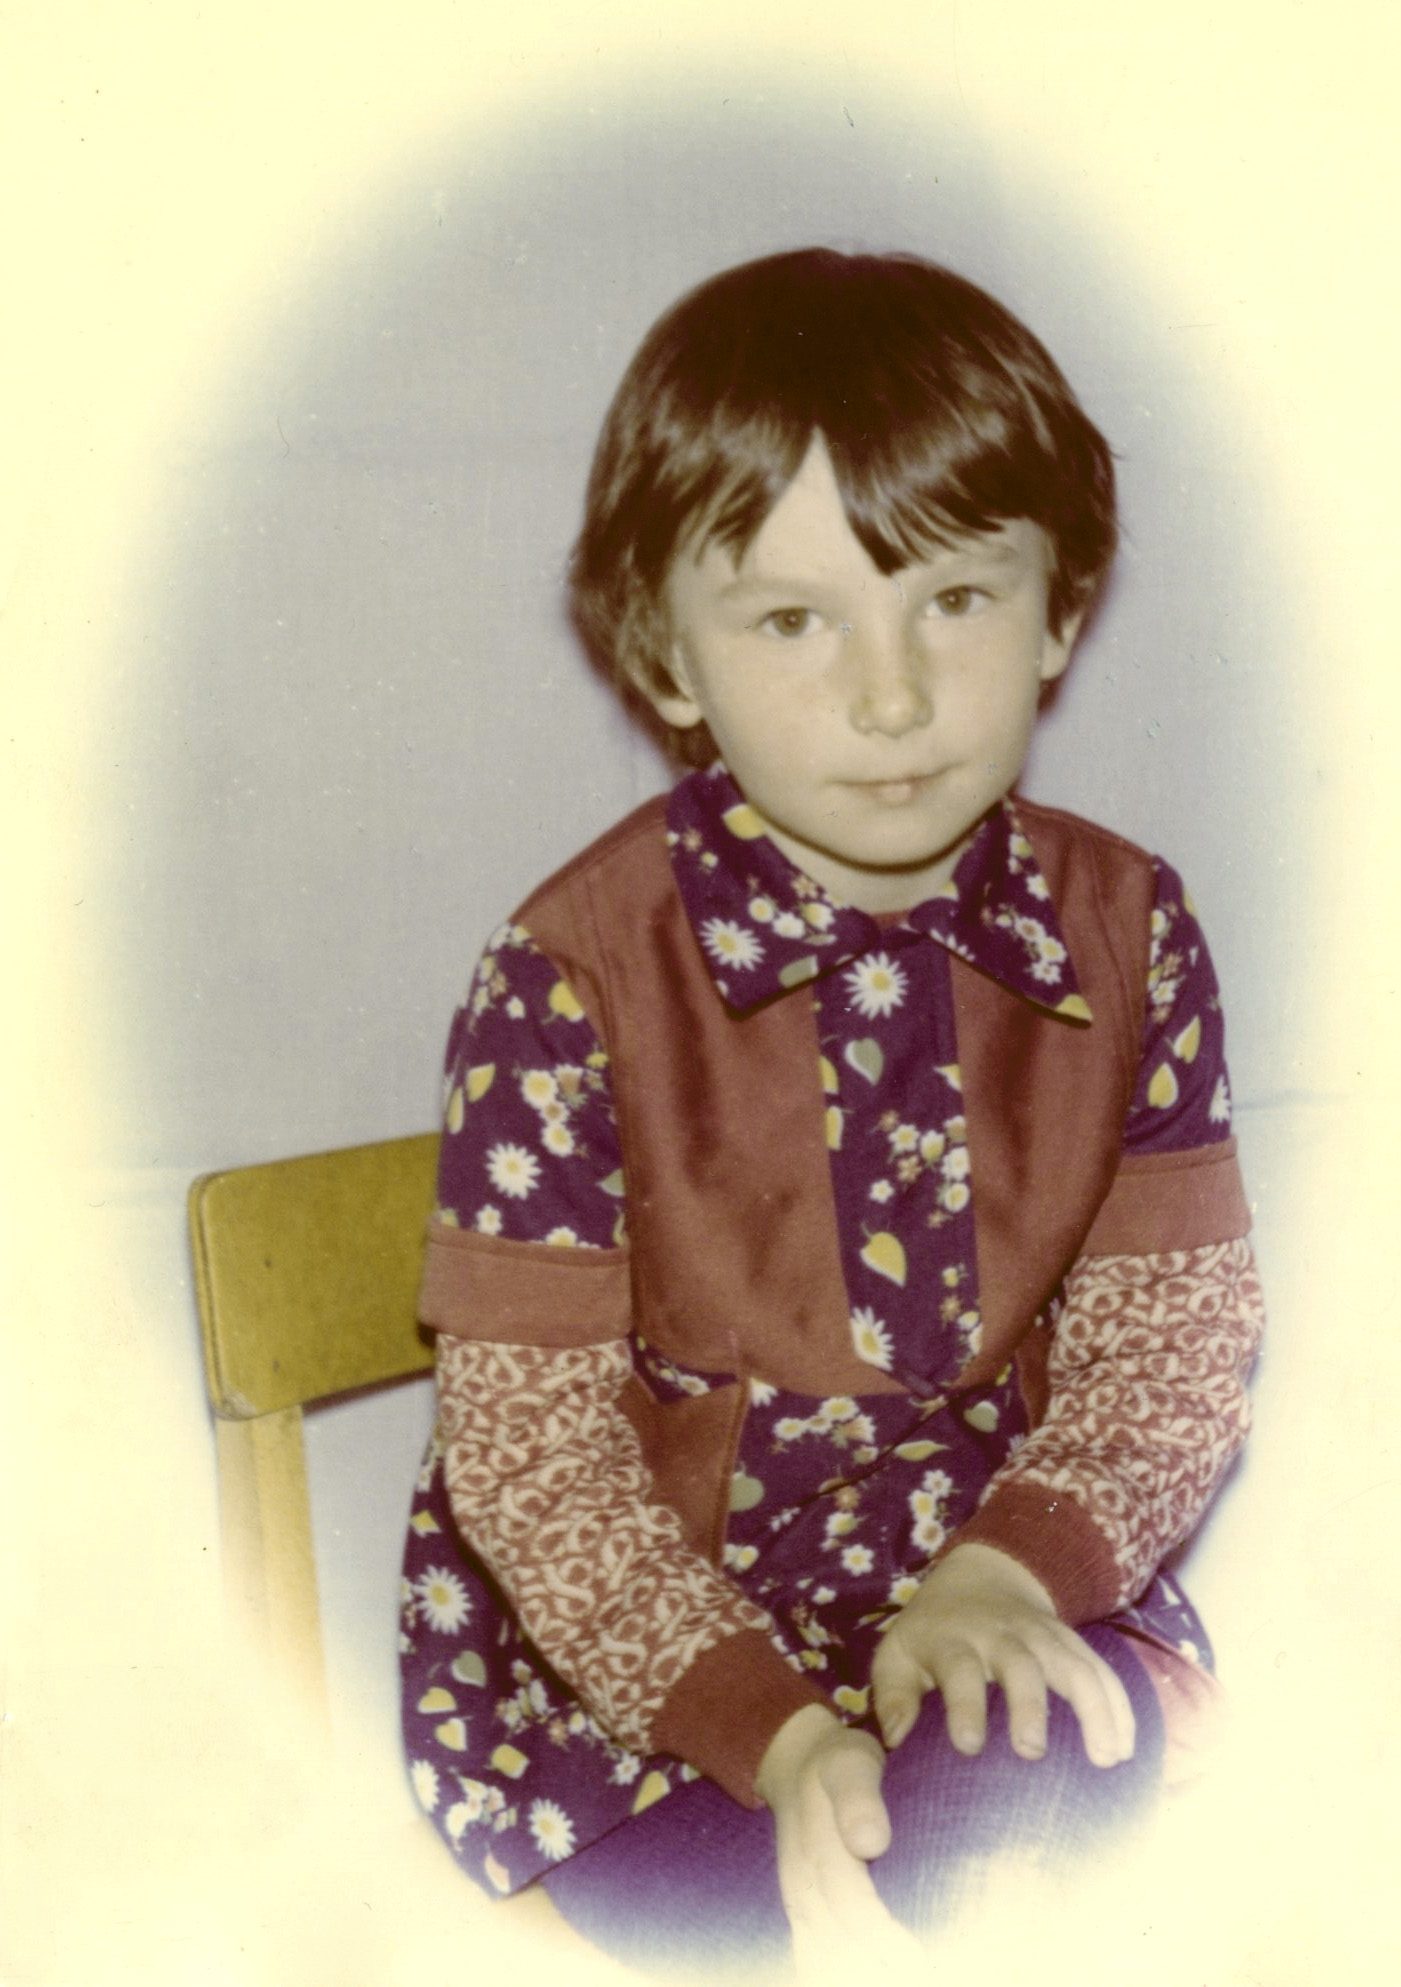
\includegraphics[width=0.4\textwidth]{photo/zuzia_swierczynska_3.jpg}
\caption{Zuzia Świerczyńska w przedszkolu}
\end{center}
\end{figure}

Potem była Szkoła Podstawowa Nr 3 bardzo chwalebnie ukończona (z czerwonym paskiem), a dalej Liceum Ogólnokształcące już w nowym miejscu, tj. w budynku po starej SP-5. Zuzia nierzadko swoim młodszym braciom matkowała, więc też oni do niej przychodzili z wieloma sprawami. Tak też Bożydar poprosił Zuzię, by mu wynalazła ciekawą książkę do poczytania, bo miał wyjechać z klasą na tzw. „Zieloną szkołę”. Zuzia potraktowała prośbę brata bardzo poważnie i znalazła mu kilkanaście ciekawych tytułów, gdyż zawsze lubiła czytać, jako urodzona humanistka. Propozycja Zuzi nie zachwyciła jednak Bożydara, który w końcu zdecydował, że na „Zieloną szkołę” zabierze sobie zbiór zadań z matematyki! Zuzia potraktowała wybór brata jak objaw szaleństwa, nienormalności, gdyż w LO za sukces uznawała ocenę dostateczną z matematyki...
\begin{figure}[!h]
\begin{center}
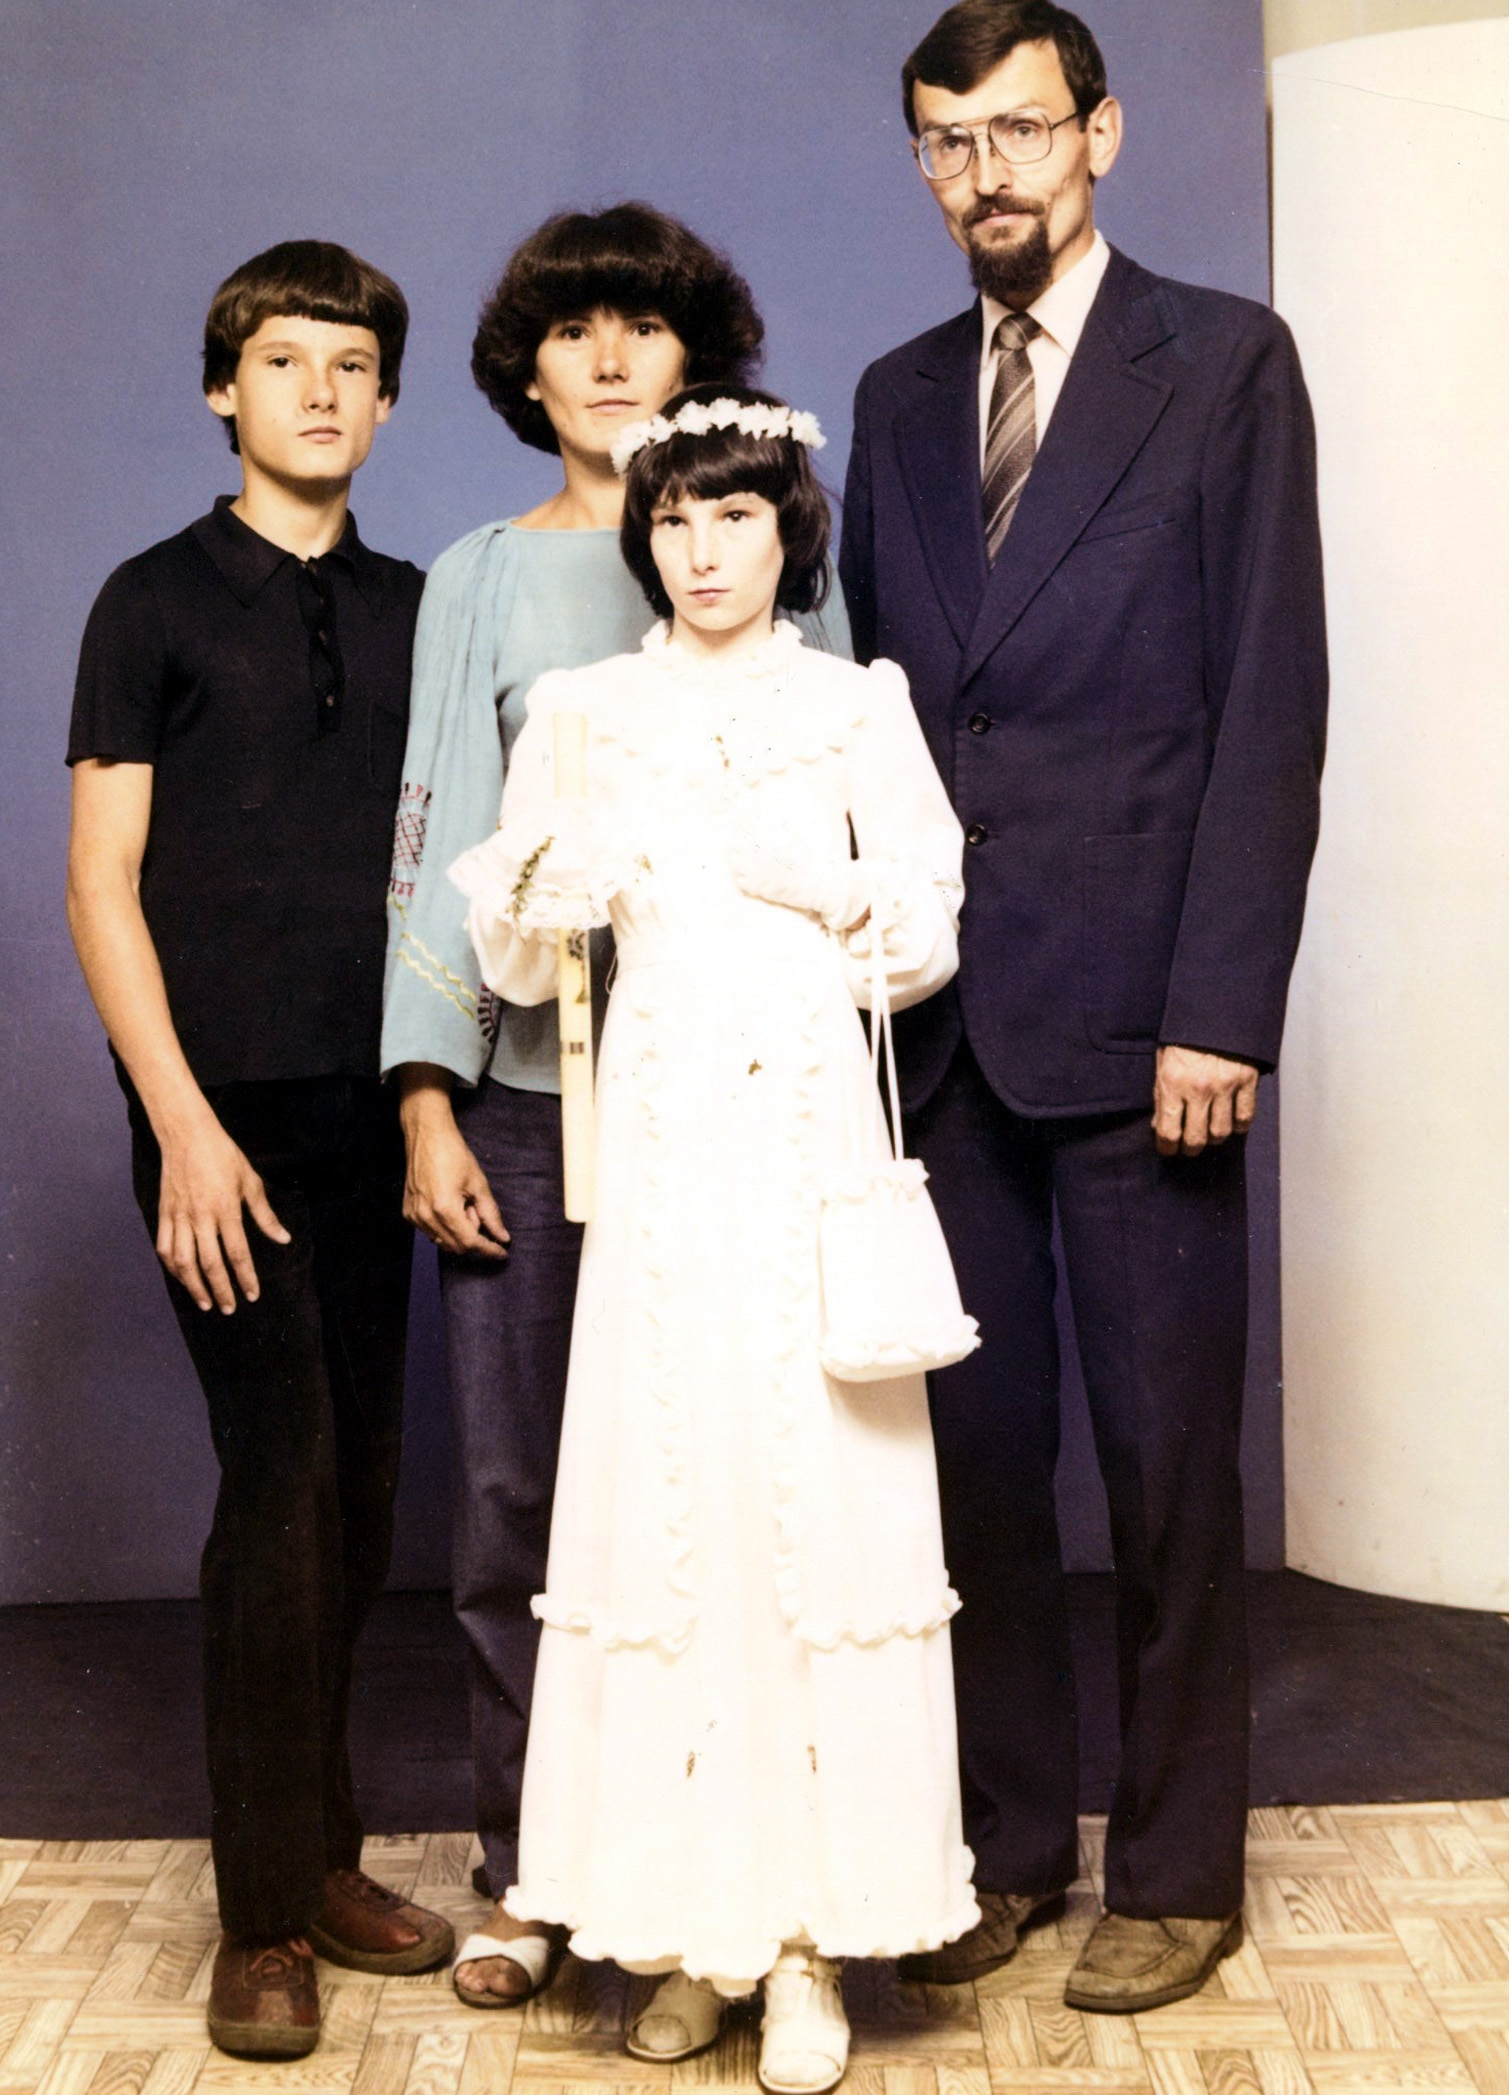
\includegraphics[width=0.5\textwidth]{photo/zuzia_swierczynska_komunia.jpg}
\caption[I Komunia św. Zuzi Świerczyńskiej]{Na zdj. od lewej: Rafał Jabłoński, Mira Jabłońska, Zuzia Świerczyńska i Czesław Świerczyński}
\end{center}
\end{figure}

Tak bardzo się nasze dzieci różnią... Wspaniały jest Bóg! Ale w jednym są moje dzieci do siebie podobne, z czego się bardzo cieszę – w służbie Bogu: każde z nich służyło do Mszy św., nawet Zuzia, co dla dziewczyny nie jest zwyczajowym zajęciem. Być może tą swoją służbą przy ołtarzu w duszpasterstwie akademickim wyprosiła sobie u Pana Boga dobrego męża oraz  śliczne i mądre dzieci...

Potem były studia z kłopotami, tak że urlop dziekański spożytkowała, zarabiając na siebie pracą w Londynie. Studia na wydziale psychologii Uniwersytetu Śląskiego ukończyła i pracuje jako psycholog w katowickich przedszkolach. Na studiach poznała dziarskiego studenta Wydziału Chemii – \textbf{Krzysztofa Kordusa urodzonego 20 września 1976 r. w Katowicach} z ojca \textbf{Franciszka} (syna Władysława i Marii z domu Macha ur. 3 października 1958~r.) i matki \textbf{Wiesławy} z domu Przybyszewska (córki Jana i Anny z domu Larek).
\begin{figure}[!h]
\begin{center}
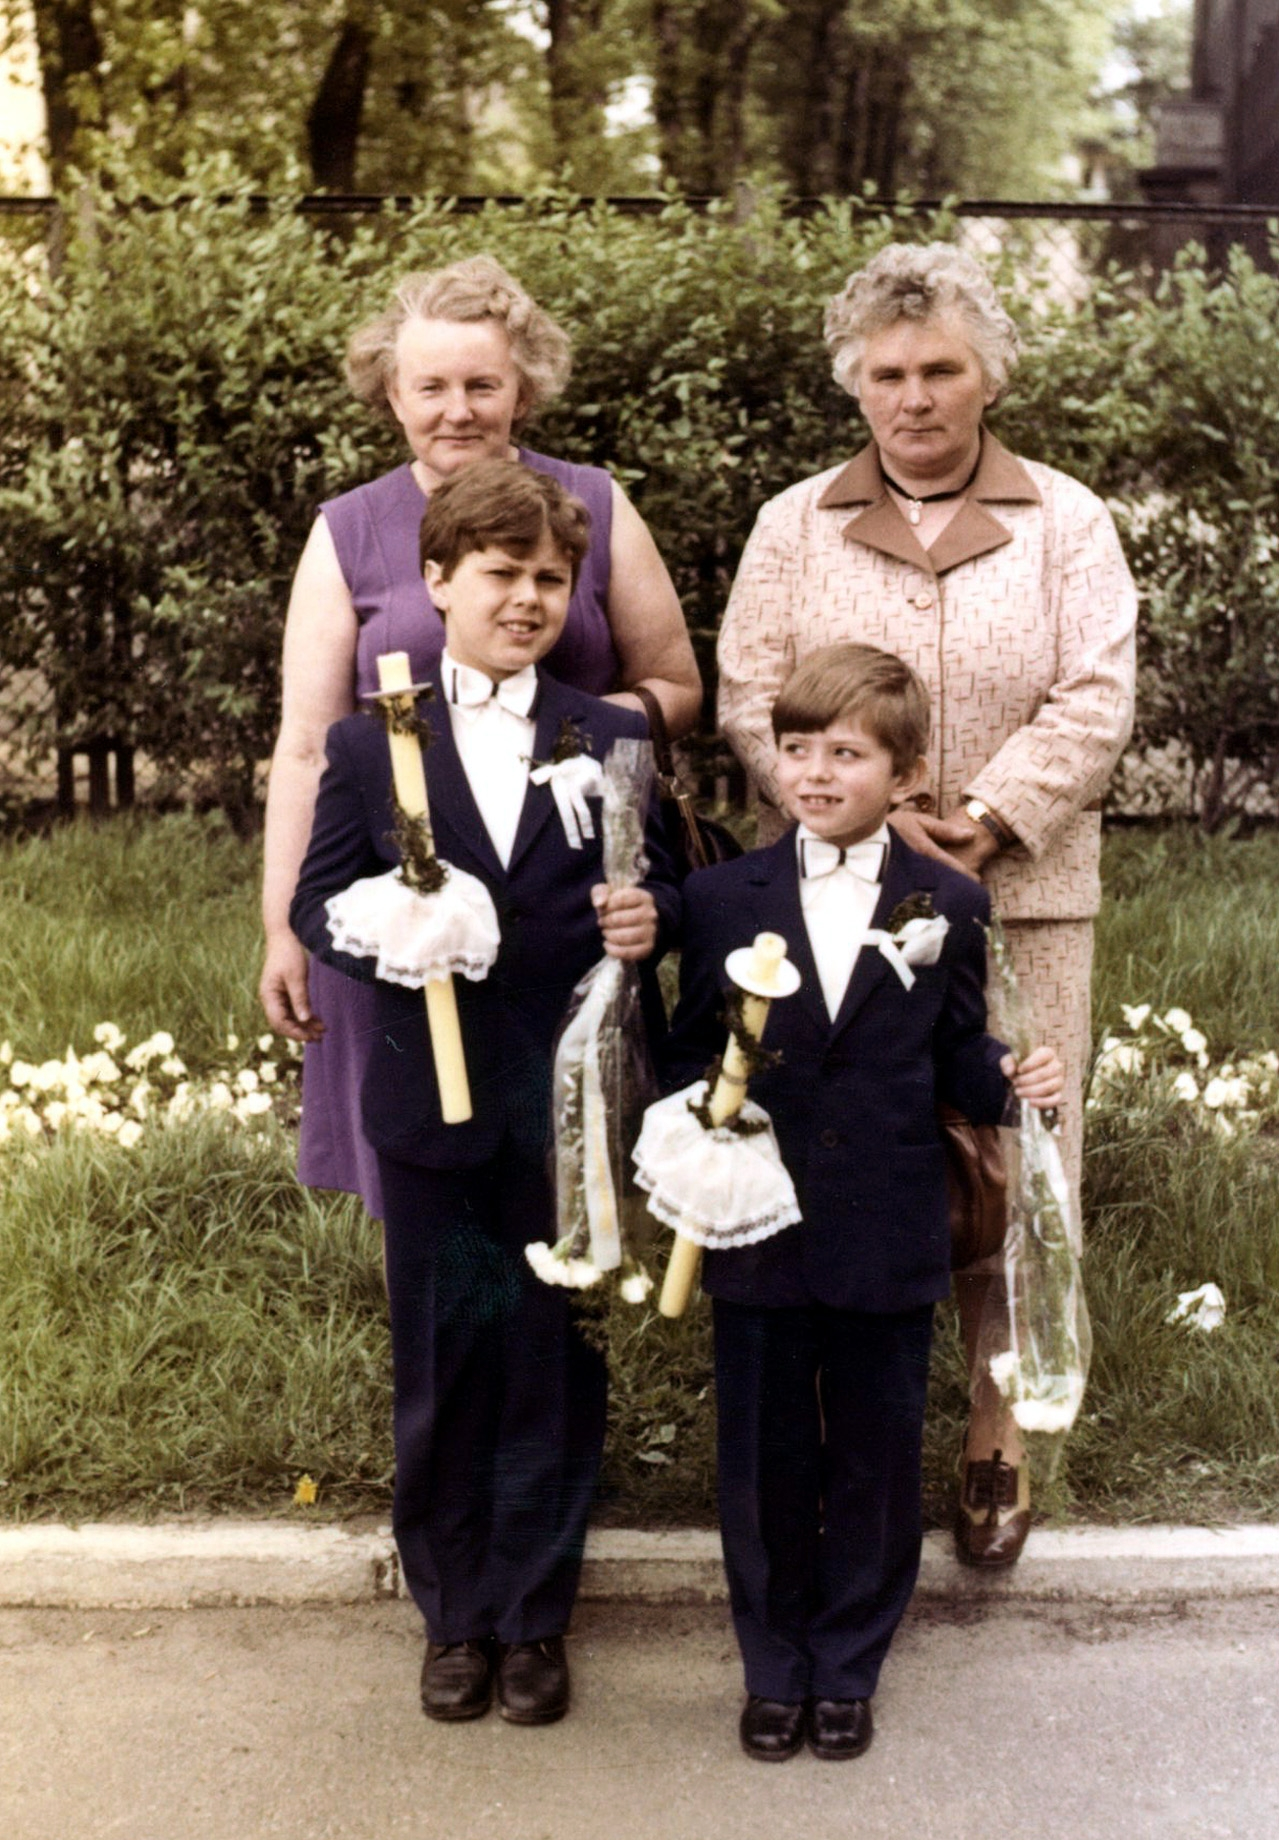
\includegraphics[width=0.4\textwidth]{photo/krzysztof_kordus_komunia.jpg}
\caption[I Komunia św. Kordusów z babciami]{Na zdj. Rafał i Krzysztof Kordusowie, za nimi babcia Anna Przybyszewska i babcia Maria Kordus}
\end{center}
\end{figure}

\begin{figure}[!h]
\begin{center}
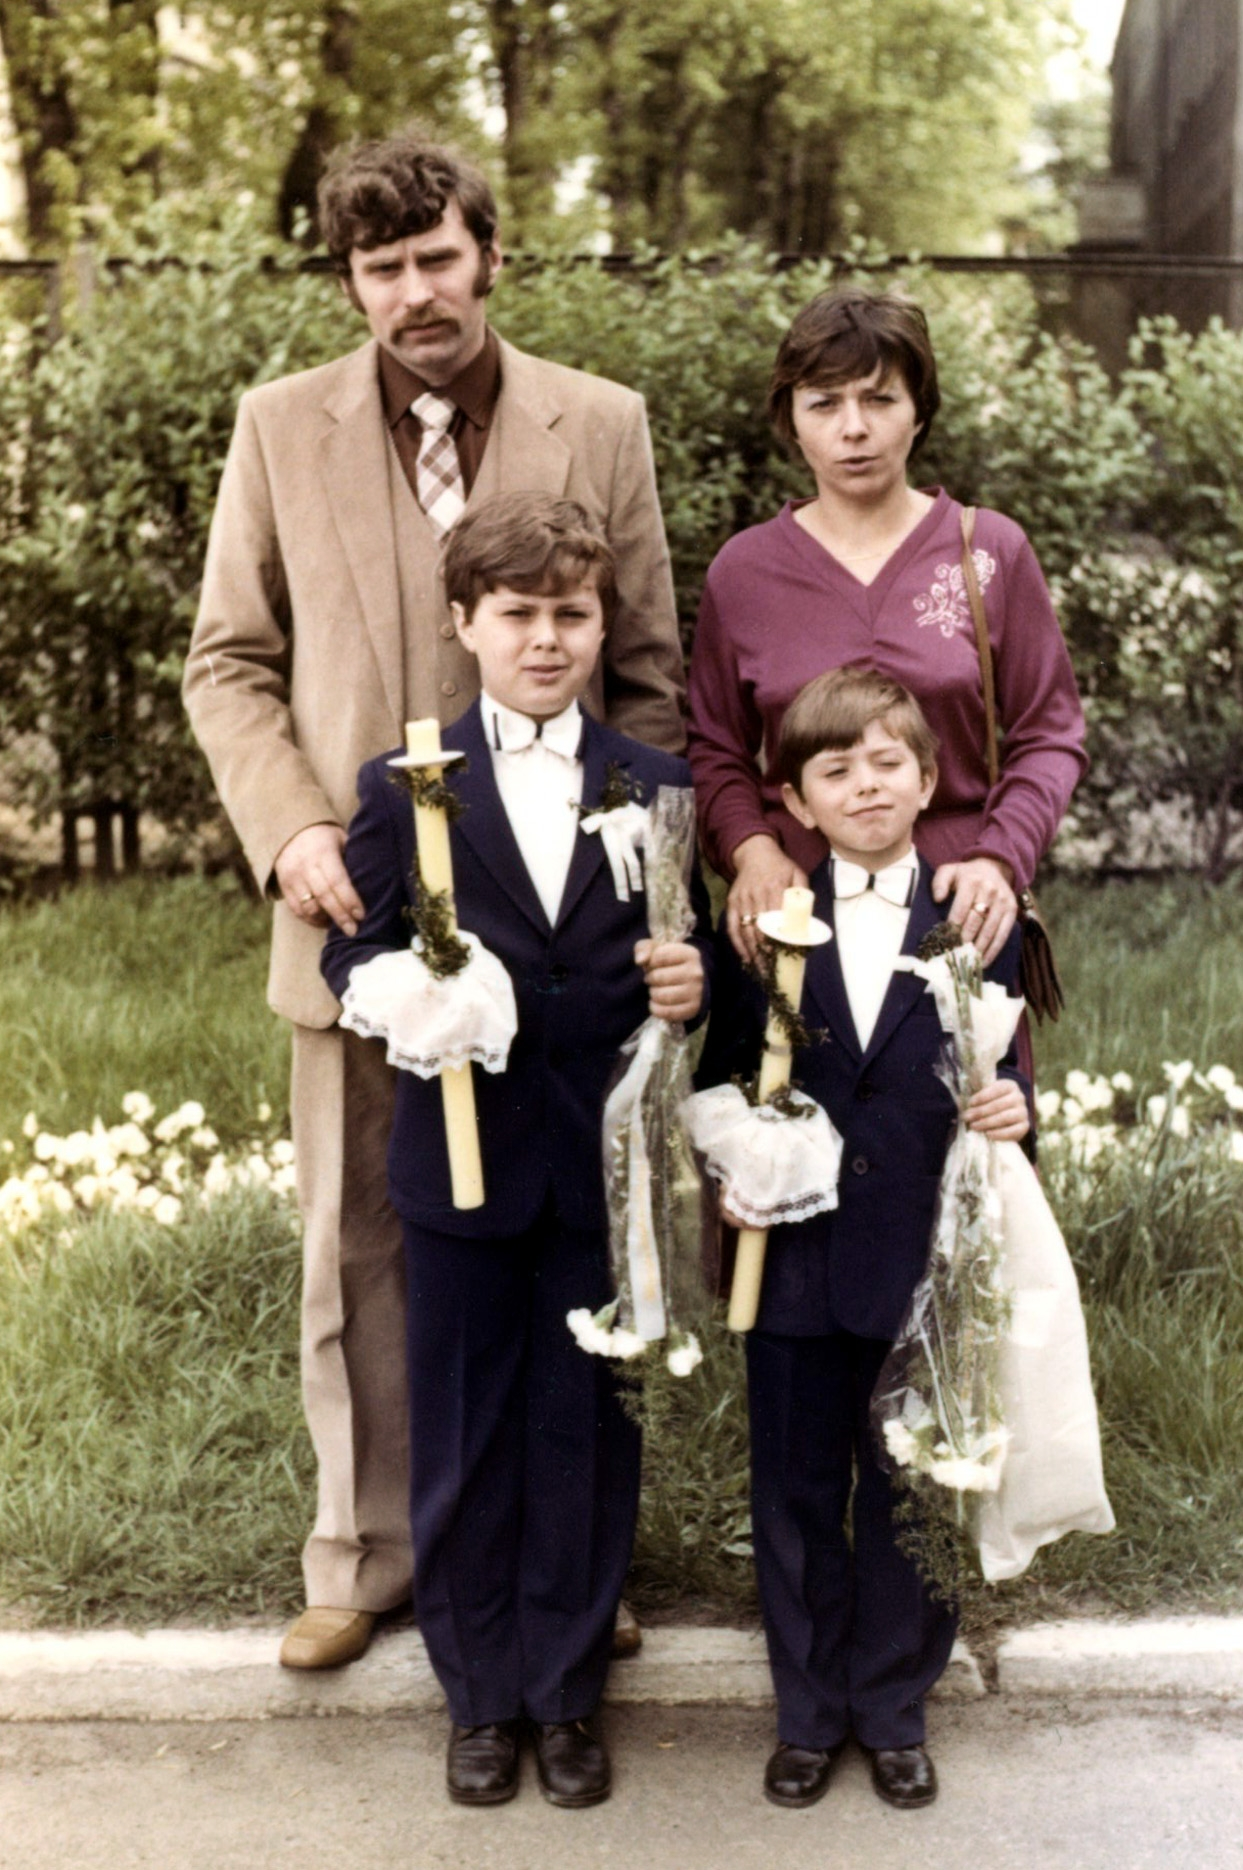
\includegraphics[width=0.4\textwidth]{photo/krzysztof_kordus_komunia_2.jpg}
\caption[I Komunia św. Kordusów z rodzicami]{Na zdj. Rafał i Krzysztof Kordusowie, za nimi Franciszek i Wiesława Kordus}
\end{center}
\end{figure}

\textbf{Pobrali się 10 sierpnia 2002 r. w kościele pod wezwaniem św. Szczepana, w Sanktuarium Matki Bożej Bogucickiej.}

\begin{figure}[!h]
\begin{center}
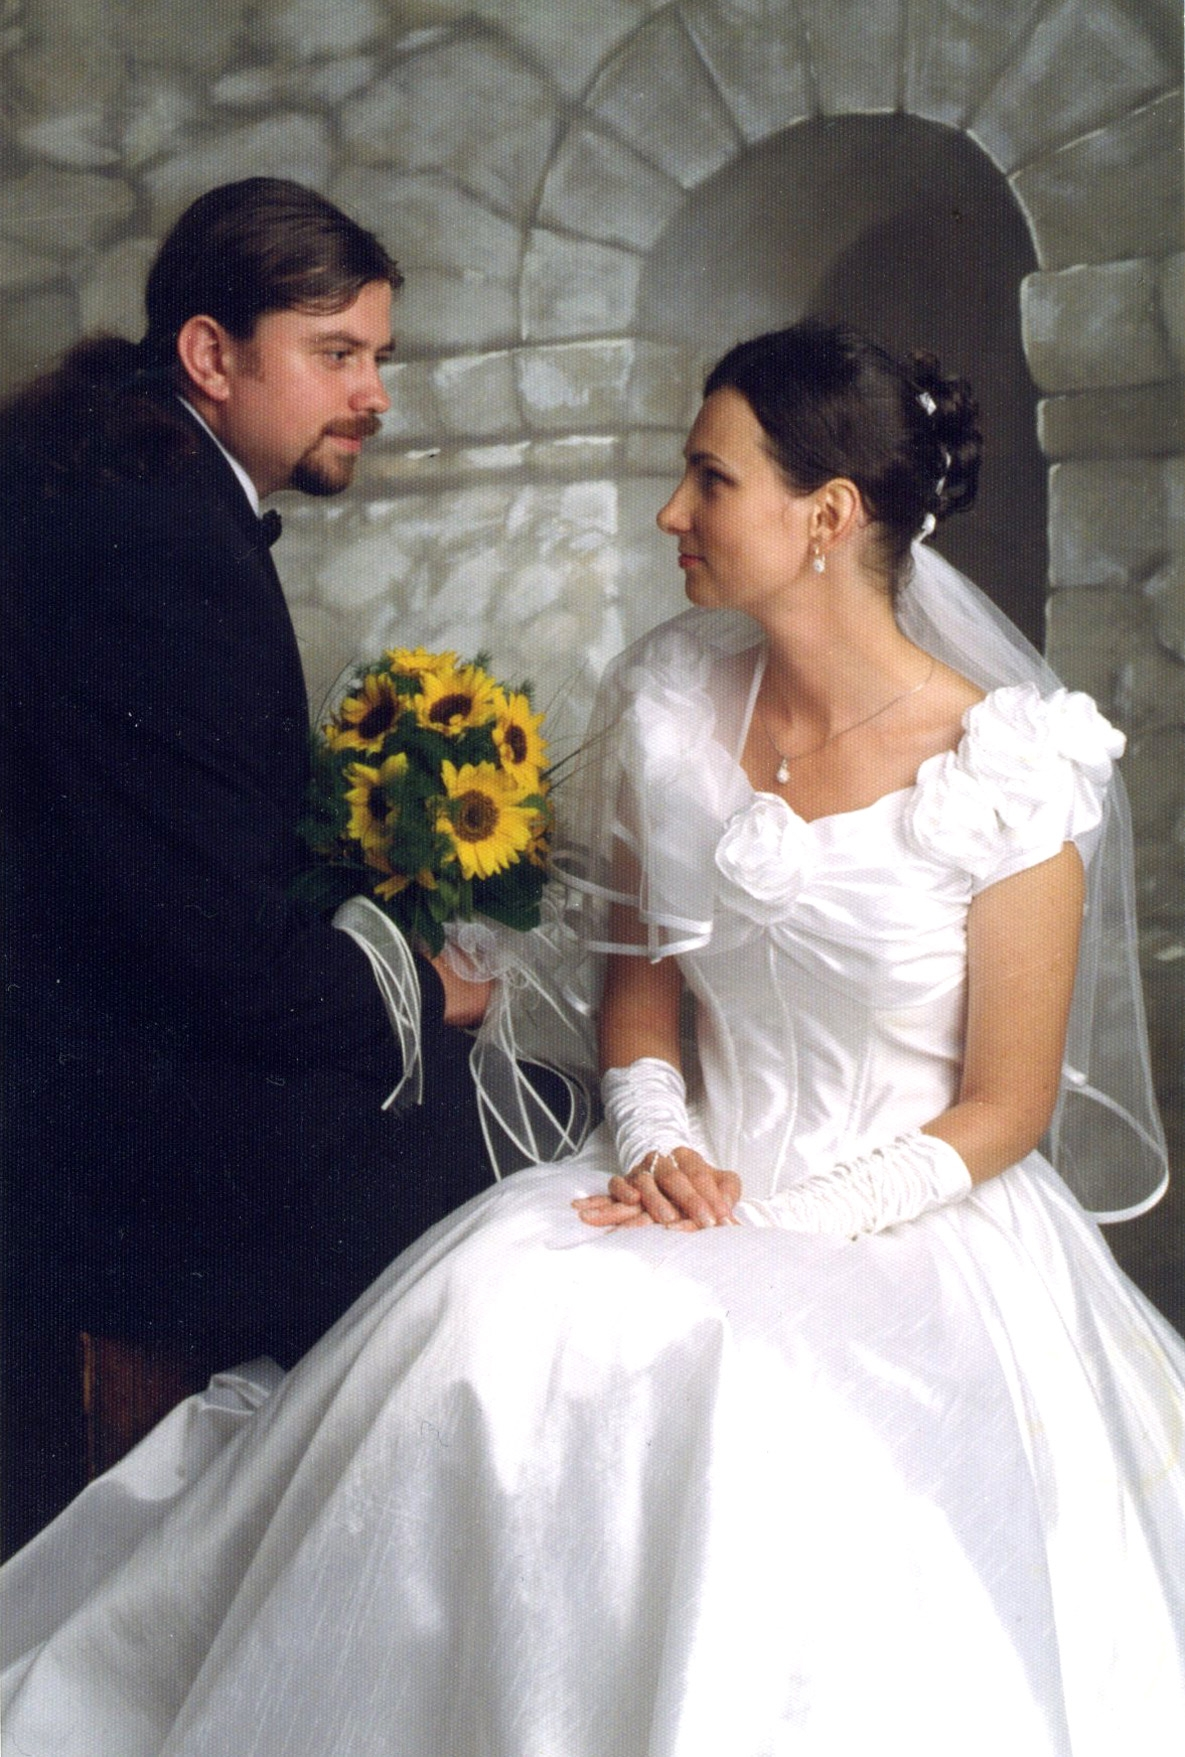
\includegraphics[width=0.45\textwidth]{photo/zuzia_krzysiek_kordus_slub.jpg}
\caption{Ślub Zuzanny Świerczyńskiej i Krzysztofa Kordusa.}
\end{center}
\end{figure}

Zamieszkali najpierw u rodziców Krzysia – przezacnych ludzi – \textbf{Franciszka} – emerytowanego policjanta \textbf{(ur. 3 października 1953 r. w Rudzie Śl. - Bielszowicach)} oraz już dziś śp. \textbf{Wiesławy} – intendentki w Przedszkolu na Osiedlu Paderewskiego \textbf{(ur. 12 maja 1953 r. w Domanicach – pow. Gostyń).}

\begin{sidewaysfigure}
\begin{center}
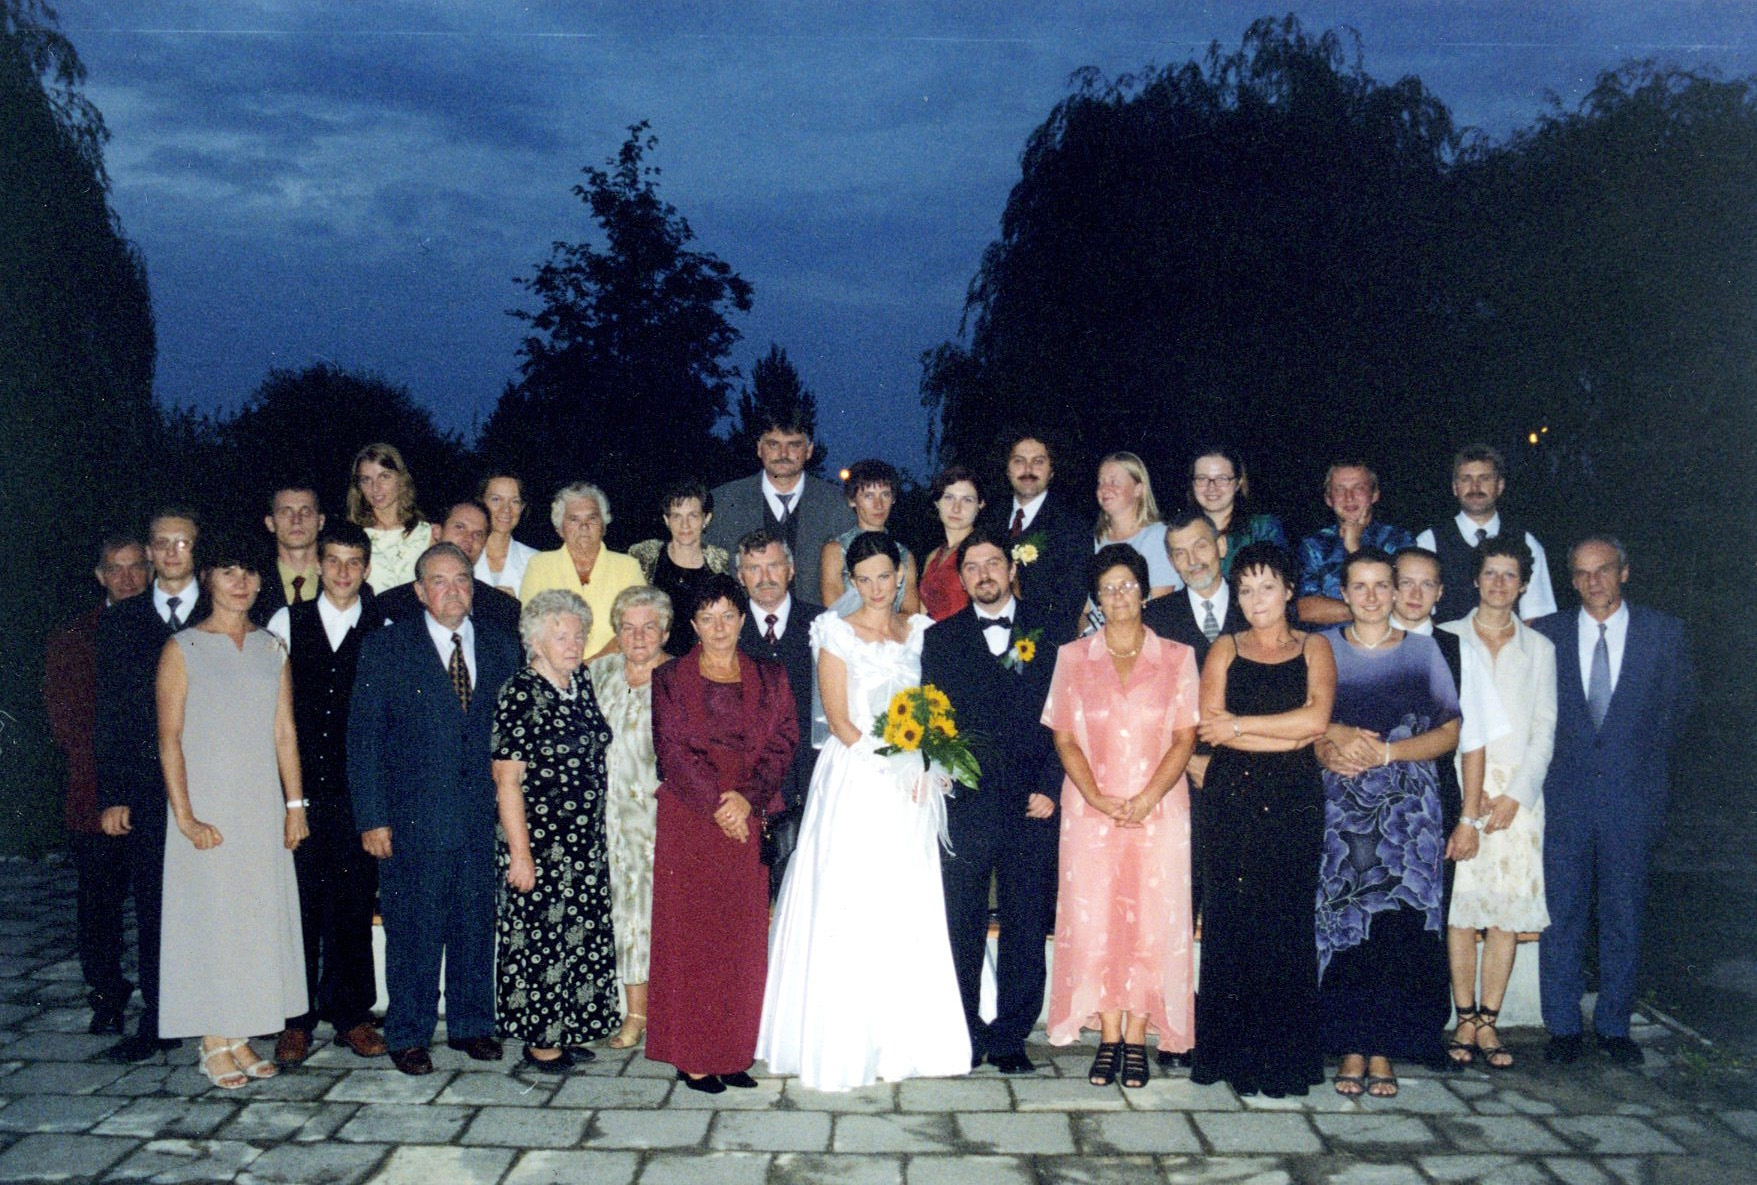
\includegraphics[width=200mm]{photo/zuzia_krzysiek_kordus_slub_2.jpg}
\caption{Ślub Zuzanny Świerczyńskiej i Krzysztofa Kordusa - zdjęcie zbiorowe. W I rzędzie od lewej: Mira Jabłońska, Piotr Świerczyński, Stanisław Kordus, Maria Kodus (babcia Krzysia), Stefania Kordus (żona Stanisława), Wiesia i Franiu Kordus, Zuzanna i Krzysztof Kordusowie, Czesława i Czesław Świerczyńscy, Renata Niepsuj, Weronika i Łukasz Pankowie, Agnieszka Głąb, Jerzy Jabłoński. W II i III rzędzie od lewej: Muzykant, Bożydar Świerczyński, Miłosz Głąb z Wiolą N., Rafał i Agnieszka Jabłońscy, Anna Przybyszewska (babcia Krzysztofa Kordusa), Weronika Gausty (siostra Franciszka Kordusa), Michał Przybyszewski (brat Wiesławy Kordus) z żoną Ewą, Natalia Potocka z Rafałe Kordusem, Patycja Malik (chrzestna Ani Kordus), Magda Ceglarska (koleżanka Zuzi), Sebastian Gausty, Adam Niepsuj.}
\end{center}
\end{sidewaysfigure}

Dość szybko nabyli mieszkanie od Michała Lutego przy ul. Sandomierskiej 19 na tym samym Osiedlu im. Jerzego Kukuczki – naszego najznakomitszego himalaisty.

Gdy zmarła nieodżałowanej pamięci mama Krzysia – Wiesława (12 lutego 2009 r. w Szpitalu w Bogucicach) Franiu zamienił się z synem mieszkaniami. Większe, przy ul. Kujawskiej 1B wzięła rozwojowa rodzina młodych Kordusów. Z ich związku przyszły na świat dwie prześliczne dziewczynki: dostojna Małgosia 11 sierpnia 2004 r. oraz 7 września 2006 r. figlarna i przebojowa Ania, obie w tym samym szpitalu, w którym przyszła na świat ich mama – Zuzia. Byłoby wspaniale, gdyby do nich dołączył jakiś mały Kordus, równie męski, jak Tata.

Krzysiu najpierw pracował w Oświęcimskich Zakładach Chemicznych i musiał codziennie kawał drogi dojeżdżać z Katowic. W tym trudnym czasie ukończył podyplomowe studia z BHP i Ochrony środowiska i dzięki nim otrzymał propozycję pracy w Fabryce Fiata w Sosnowcu, gdzie pełni funkcję behapowca i jest przez szefostwo doceniony. Jego hobby to piłka nożna (na którą każdego tygodnia stara się parę godzin poświęcić) oraz ryby akwariowe, dzięki czemu ich mieszkanie zyskało na kolorowych akwariach starannie utrzymanych. Dzielny człowiek, prawdziwy mężczyzna zatroskany o rodzinę, lubiący gotować, towarzyski i szybki w działaniu.
\begin{figure}[!h]
\begin{center}
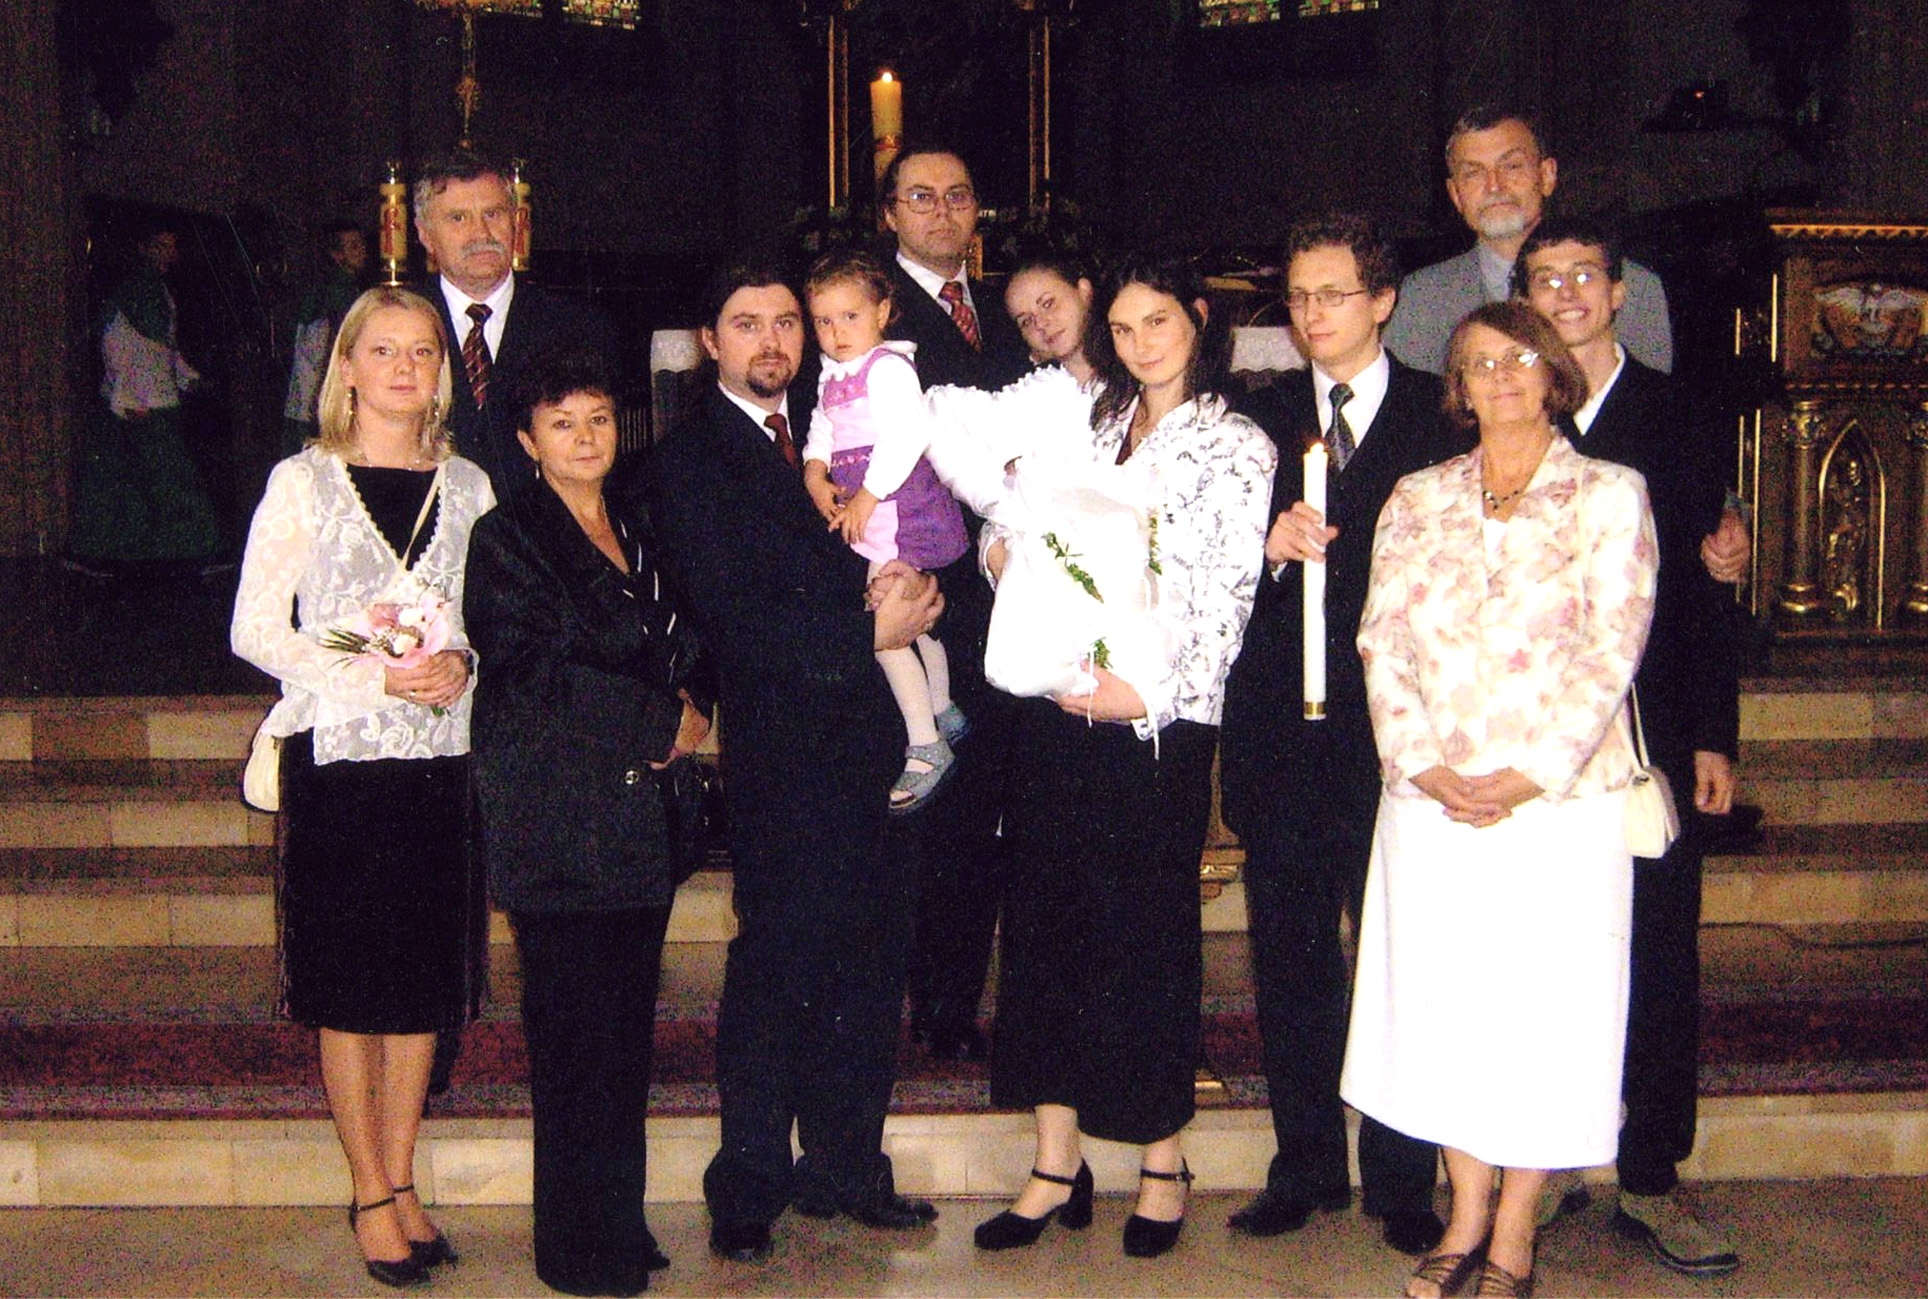
\includegraphics[width=0.9\textwidth]{photo/ania_kordus_chrzest.jpg}
\caption[Chrzest Ani Kordus]{Na zdj. od lewej: Patrycja Malik, Franciszek i Wiesława Kordusowie, Krzysiu z Małgosią Kordus, Rafał Kordus z Agnieszką, Zuzia Kordus z Anią na ręku, Bożydar Świerczyński (ojciec chrzestny), Czesława, Czesław i Piotr Świerczyńscy}
\end{center}
\end{figure}

Ma brata Rafała, który uzyskał tytuł doktorski na Akademii Rolniczej we Wrocławiu. Tam też mieszka wraz ze swą żoną Agnieszką. Zuzia próbuje, jak onegdaj Krzysiu, przekwalifikować się, gdyż w dobie szukania oszczędności prezydent miasta Katowice może obciąć przedszkolom etaty psychologa. Podjęła więc studia podyplomowe, które ją drogo kosztują, ale może dadzą jej stabilniejsze źródło dochodów. Mają samochód, który im pomaga być mobilnymi, więc w miarę często bywają z dziewczynkami w Mirowie oraz w Stryszawie, gdzie rodzice Krzysia wybudowali sobie domek letniskowy z poddaszem użytkowym w stylu podhalańskim.
\begin{figure}[!h]
\begin{center}
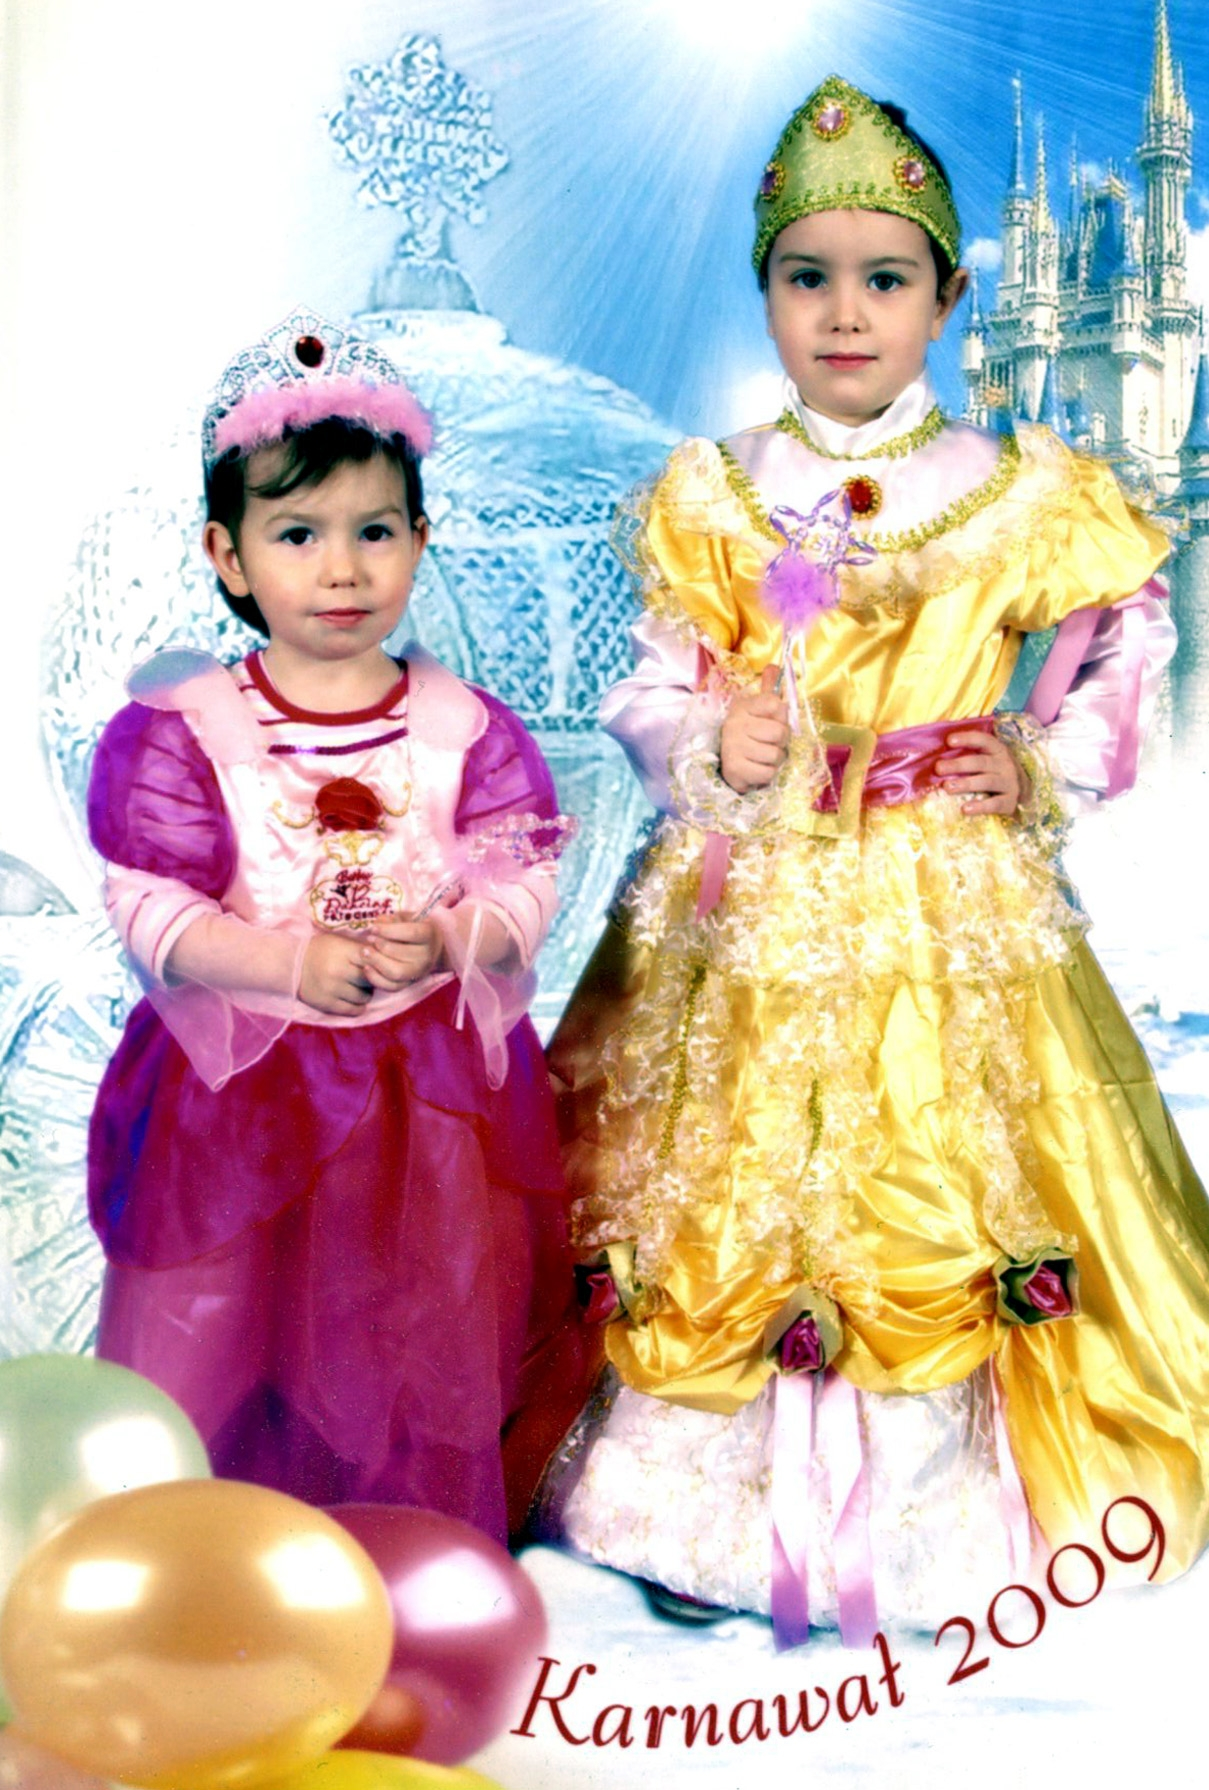
\includegraphics[height=90mm]{photo/gosia_ania_kordus_1.jpg}
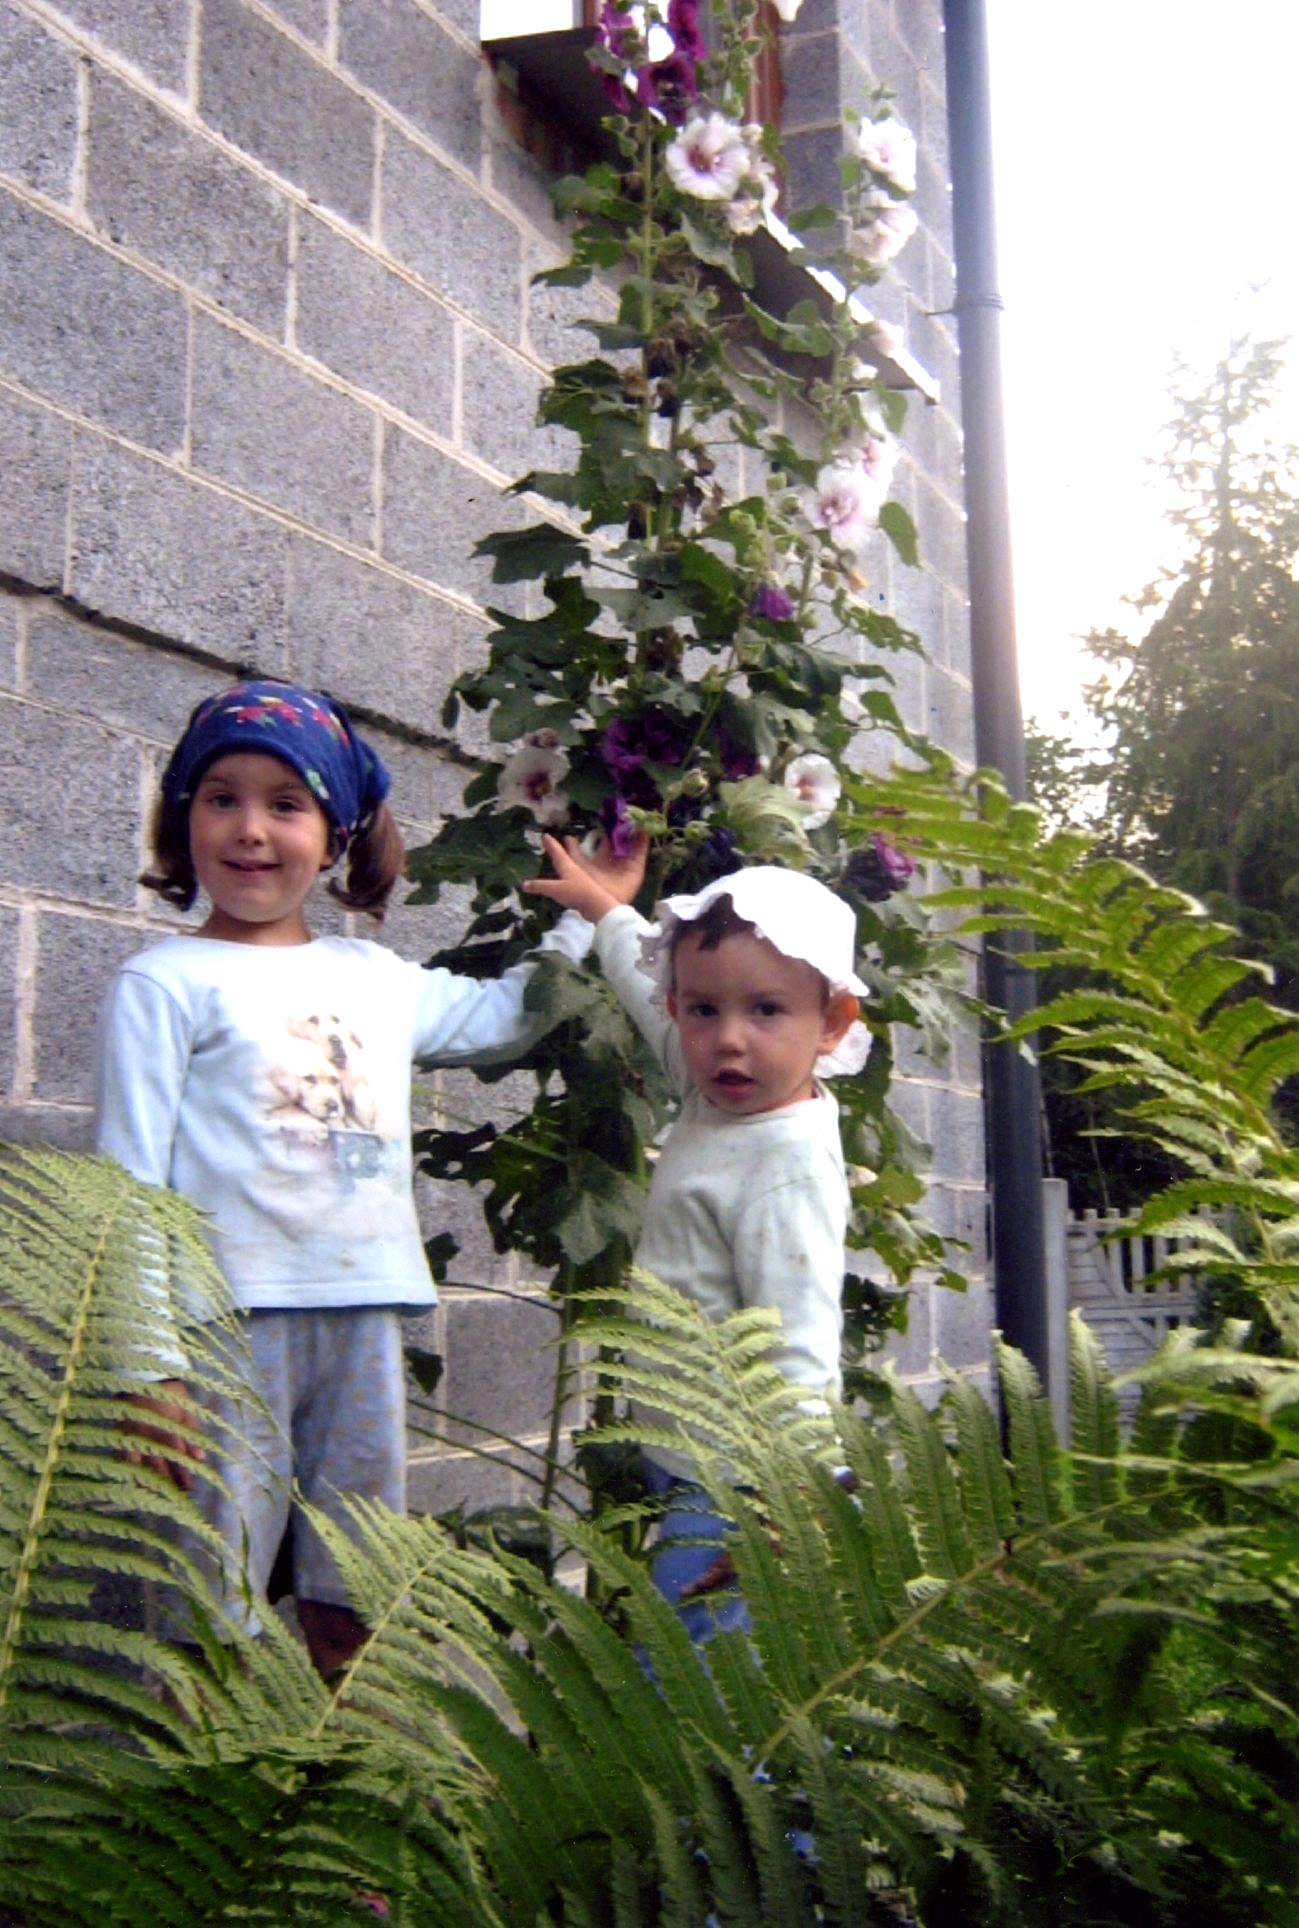
\includegraphics[height=90mm]{photo/gosia_ania_kordus_2.jpg}
\caption{Ania i Gosia Kordusówne}
\end{center}
\end{figure}









\clearpage

\textbf{Bożydar to nasze drugie dziecko i mój pierworodny syn,} który miał pecha, że w czwartym miesiącu życia, tj. 13 grudnia 1981 r. pachołek Rosji, niejaki Jaruzelski wprowadził stan wojenny, więc większość aktywnych i odważnych działaczy „Solidarności” internowano w więzieniach zaś rodzinom internowanych dano odczuć, że są obywatelami trzeciej kategorii. Wasza Mama dzielnie znosiła te szykany i znalazła czas i siły, by mnie, mimo swojego odmiennego stanu kilka razy odwiedzić w więzieniu. W tym stanie rzeczy maleńki Bożyś tłumione przez mamusię lęki najdotkliwiej odczuwał. Urodził się 13 maja 1982 r. w Katowicach w piątą miesięcznicę naszego internowania, ale przede wszystkim w pierwszą rocznicę cudownego ocalenia Jana Pawła II.
\begin{figure}[!h]
\begin{center}
\includegraphics[width=0.6\textwidth]{photo/zuzia_bozydar_swierczynscy.jpg}
\caption{Bożydar i Zuzia Świerczyńscy}
\end{center}
\end{figure}

Nie wiem czy Zuzia pamięta, jak przemodliliśmy z nią cały różaniec (dziecko wtedy sześcioletnie) w intencji ocalenia życia Ojca Świętego. 13 maja 1982 r. koledzy fetowali kolejną miesięcznicę swego zniewolenia, ja zaś z moim serdecznym przyjacielem – Waldkiem Mikołowiczem odmawiałem w dziękczynieniu Bogu w Trójcy Jedynemu i Niepokalanej – „Anioł Pański”. W tym właśnie czasie, krótko przed dwunastą przyszedł na świat mój, nasz Boży Dar! Moje Drogie Dzieci, pamiętajcie, że Bóg nigdy nie da się prześcignąć ludziom w łaskawości, w dobrodziejstwach... Ochrzczony był w kościele pw. św. ap. Piotra i Pawła w Katowicach (tam gdzie Zuzia 7 lat wcześniej).
\begin{figure}[!h]
\begin{center}
\includegraphics[width=0.6\textwidth]{photo/bozydar_swierczynski_1.jpg}
\caption{Bożydar Świerczyński}
\end{center}
\end{figure}

Nasz kochany \textbf{Bożydar} już przyszedł na świat pełen niepokoju, a jeszcze źle leczony przez B. Malickiego zbyt silnymi antybiotykami cierpiał na chroniczne zapalenie górnych dróg oddechowych. Tę diagnozę postawił w trzecim roku jego życia ksiądz Kilianek, którego mi polecił ojciec Oskar Puszkiewicz – franciszkanin. Stawiał on diagnozę na podstawie zapisu, jaki zostawia organizm człowieka w tęczówce oka pacjenta ( takie diagnozowanie nazywa się irydologią od iris, co po grecku znaczy tęcza), wszystkie choroby, złamania, traumy są tam zapisane. I to potrafił odczytać \textbf{ksiądz Kilianek}, który brał za to niewielką opłatę na prowadzenie zielarskiej apteki. Powiedział on, że Bożydar ma uszkodzone nerki z powodu zbyt silnych antybiotyków, jakie zostały mu podane już w pierwszych miesiącach życia. Tak uszkodzone nerki niedoczyszczały krwi z moczu, na którą układ oddechowy reagował jak na zainfekowaną krew, w wyniku czego cały organizm stawał do walki z pozorną infekcją, na co lekarz reagował silniejszymi antybiotykami itd. Ksiądz Kilianek przepisał zestaw  kilkunastu ziół, z którego tylko siedem można było nabyć w Herbapolu. Resztę na podstawie książek i szukania po polach i lasach zdobyłem sam. Ostatnim była cetraria islandica, czyli płucnica islandzka, którą odkryłem na śródleśnych polanach Mirowa. Bożydar pierwszy kubek tej mikstury wypił duszkiem i z miesiąca na miesiąc stawał się coraz zdrowszy, tak że nareszcie do zerówki uczęszczał w zasadzie bez przerwy.
\begin{figure}[!h]
\begin{center}
\includegraphics[width=0.5\textwidth]{photo/bozydar_swierczynski_komunia.jpg}
\caption[I Komunia św. Bożydara z dziadkami]{Na zdj. siedzą: babcia Radinka i Irena Lehman, między nimi Bożydar, za nimi stoją: dziadek Benedykt Świerczyński, rodzice Czesława i Czesław oraz dziadek Franciszek Głąb.}
\end{center}
\end{figure}

Te choroby tak go wyczerpały, że dopiero w trzecim roku życia zaczął mówić! Mamusia była bardzo zaniepokojona o jego zdrowie, lecz ja byłem pełen ufności w Bożą Opatrzność. I doczekała się mamusia, gdy Bożydar już w zerówce okazywał swe nadzwyczajne uzdolnienia matematyczne! Zanim którekolwiek dziecko z grupy zdołało odpowiedzieć już Bożyś wyrywał się z gotowym rozwiązaniem. Pamiętam, jak w obecności trzyletniego Bożysia, jeszcze nie mówiącego śpiewałem w średnim pokoju „Ciebie Boże wielbimy” na co on reagował przeogromną, niebiańską radością! Można by za Panem Jezusem powiedzieć: „Błogosławiony jesteś Bożydarze, bo nie kazały ci się radować tą pieśnią ani ciało ani krew, lecz Ojciec Niebieski.”(Mat. 16.16).
\begin{figure}[!h]
\begin{center}
\includegraphics[width=\textwidth]{photo/bozydar_swierczynski_komunia_2.jpg}
\caption[I Komunia św. Bożydara -- zdjęcie zbiorowe]{Na zdj. od lewej w I rzędzie: Kasia i Irek Wilkowie, babcia Radegunda Świerczyńska, Bożydar, Irena Lehman, Agnieszka Głąbówna, dziadek Franciszek Głąb, dziadek Benedykt Świerczyński, w II rzędzie: Mirosław Głąb (chrzestny), Zofia Prele (chrzestna), mama Czesława, Basia Wilk, tata Czesław, Marek Lehman z żoną Małgosią, Tomasz Świerczyński i Miłoszek Głąb.}
\end{center}
\end{figure}

Nie zatrać mój drogi Bożydarze tego wielkiego i rzadkiego błogosławieństwa jakimś bezbożnym czynem lub myślą...

Bożydar od dziecka był skromny, gotowy zaprzeczać czyimkolwiek pochwałom. Gdy na drugich lub trzecich urodzinach Ani Kordus, Bożydar wykonał jakąś przestrzenną układankę, której reszta nas gości nawet napocząć właściwie nie potrafiła, zacząłem wysławiać jego niezwykłe uzdolnienia, na co ów chwalony kategorycznie zakazał mi tej laudacji...

\begin{figure}[!h]
\begin{center}
\includegraphics[width=0.6\textwidth]{photo/bozydar_swierczynski_michal_socha.jpg}
\caption{Bożydar Świerczyński i Michał Socha}
\end{center}
\end{figure}

Obawiam się, że na rynku pracy z taką skromnością nie pozwoli się poznać pracodawcom jako wykonawca z najwyższej półki, chyba że Natalia będzie mu robiła reklamę, jak żona Pendereckiego, dzięki czemu jest jej Krzysztof poważany i ceniony w najznamienitszych filharmoniach świata. Gdy się skończyła na Politechnice matematyka, która była postrachem przytłaczającej większości studentów, Bożydar po raz pierwszy miał „tylko” czwórkę jako średnią ocen w całym kilkunastoletnim toku nauczania. Do tej pory zawsze piątki.
\begin{figure}[!h]
\begin{center}
\includegraphics[width=0.7\textwidth]{photo/bozydar_swierczynski_1_kl_traugutt.jpg}
\caption{Bożydar Świerczyński - I klasa II LO im. R. Traugutta}
\end{center}
\end{figure}

Na piątym roku studiów nasz Bożydar poznał uroczą Natalię z Gruszków ur. 15 grudnia 1982 r. w Ziębicach. Moje dzieci często przychodziły do mnie bym ze zdjęcia ich wybrańca bądź wybranki odczytał jej lub jego cechy charakteru zapisane w oczach i rysach twarzy. O Natalii wypowiedziałem się w samych superlatywach. Zresztą – tak mi się wydaje – od razu przypadliśmy sobie do serca.

\textbf{Bożydar} na poważnie zajął się swoją Wybranką Serca, tak że \textbf{się z nią 4~września 2010~r. ożenił w Ziębicach}.

Lecz najpierw pojechał za nią do Belfastu, bo tam znalazła pracę. Mieszkali w Belfaście od 2008 r. (Bożydar od listopada) do września 2010 r.

0d października tego roku mieszkają już w Edynburgu – stolicy Szkocji. Bożydar jest zatrudniony w Dundee, natomiast Natalia pracuje obecnie w Edynburgu.

\textbf{Natalia} ukończyła Wydział Chemiczny Politechniki Wrocławskiej. \textbf{Jest pierwszym dzieckiem Wiesława Gruszki ur. 14 lipca 1957 r. w Ziębicach} z ojca Józefa i matki Heleny oraz \textbf{Małgorzaty Gruszki z domu Kluz ur. 12 października 1961 r. w Ząbkowicach Śląskich} z ojca Józefa i matki Zofii. Po Natalii przyszedł na świat 14 sierpnia 1984 r. w Ząbkowicach Śl. Radosław żonaty z Martą Gottfried. W Dusznikach Zdroju przyszedł na świat 12 września 1988 r. Krzysztof Gruszka. Po nim w Ziębicach 8 września 1990~r. urodziła się Alicja. Najmłodszym w rodzeństwie – jak u nas – jest Piotr urodzony 18 lipca 1993~r. w Ząbkowicach Śląskich. Korzenie rodziny Gruszków sięgają ziem wschodnich II Rzeczypospolitej.











\clearpage

\textbf{Piotruś}, to nasze najmłodsze dziecię i najbardziej bojowe. Zaczął chodzić i mówić grubo przed ukończeniem roku życia. Jego chrzestni też przebojowi, ale i on sam przyszedł na świat najcięższy i najsilniejszy, czego dał wyraz wydając do słuchawki telefonu trzymanej przez babkę Lehmankę donośny wrzask. \textbf{Działo się to 4 kwietnia 1987 r. w Katowicach w szpitalu przy ul. Raciborskiej.} Kiedy ośmioletni Bożyś przybiegł do mnie z wiadomością, że po drugiej stronie bloku biją Piotrusia, ja w te pędy za blok, lecz zanim znalazłem się na miejscu zajścia, podbiegł trzyletni Piotruś zapłakany, na co Bożyś do niego z wyrzutem: „Dlaczego nie uciekałeś?”, na co Piotruś: „Bo się biłem.” 
\begin{figure}[!h]
\begin{center}
\includegraphics[width=0.5\textwidth]{photo/bozydar_piotr_swierczynscy_1.jpg}
\caption{Bożydar i Piotr Świerczyńscy}
\end{center}
\end{figure}

Ten krótki dialog dobrze ich charakteryzuje. Starszy ostrożny, unikający walki, lecz nie za wszelką cenę, szukający póki co sojuszników i bezpiecznych rozwiązań, młodszy Piotruś bojowy, atakujący, gotowy natychmiast do walki o swoje i o sprawiedliwość. Zawsze niezwykle ambitny, walczący o pierwsze miejsca i odważny. 

\begin{figure}[!h]
\begin{center}
\includegraphics[width=0.7\textwidth]{photo/piotr_swierczynski_chrzestni.jpg}
\caption[Piotr Świerczyński z chrzestnymi i bratem]{Na zdj. od lewej: Krzysiu Karoń, Piotruś Świerczyński, Joasia Jarzębińska i Bożydar Świerczyński.}
\end{center}
\end{figure}

Gdy mu się należy pierwsze miejsce, to gotów się o nie upomnieć. Nie jest pyszałkiem, ale krzywdy nie da sobie zrobić! Dobry Boże wspieraj go w walce, a przeciw niegodziwościom złego ducha poślij mu na pomoc Maryjo, jego wielka ze św. Piotrem Współpatronko - hufiec Aniołów.

\begin{figure}[!h]
\begin{center}
\includegraphics[width=0.4\textwidth]{photo/piotr_swierczynski_1.jpg}
\caption{Piotr Świerczyński z obrazem Matki Bożej Mrzygłodzkiej}
\end{center}
\end{figure}

Piotruś każdą szkołę kończył chwalebnie, z wyróżnieniem i nagrodami. Teraz równie chwalebnie kończy studia prawnicze na Katolickim Uniwersytecie Lubelskim, obronił pracę magisterską na piątkę z wyróżnieniem. 


\begin{figure}[!h]
\begin{center}
\includegraphics[width=0.7\textwidth]{photo/piotr_swierczynski_2.jpg}
\caption[Piotr Świerczyński w służbie ołtarza]{Na zdj. od lewej: Piotr Świerczyński w albie lektora, przy ołtarzu ks. prałat Zdzisław Skrzek, ks. arcybiskup Stanisław Nowak, ks. Krzysztof Tkacz.}
\end{center}
\end{figure}

Poznał tam swoją wybrankę \textbf{Justynę} (to imię tak pięknie się kojarzy z istotą jego zawodu) \textbf{Sobczykównę}, która przyszła na świat \textbf{3 września 1987 r. w Kielcach} z ojca \textbf{Sławomira (urodzonego w Kielcach 4 sierpnia 1954 r. z ojca Jana i matki Cecylii Toporek)} oraz matki \textbf{Anny z Murczyńskich Sobczykowej (urodzonej 8 lipca 1960 r. w Krakowie z ojca Józefa i matki Marianny Placek Murczyńskiej Cierlik).} Kończy chwalebnie studia psychologiczne, tam gdzie Piotruś, tj. na KUL-u. Będą zawierać związek małżeński jako wyróżnieni magistrowie i to w katedrze kieleckiej pod wezwaniem Wniebowzięcia Matki Bożej (Łaskawej)!
\begin{figure}[!h]
\begin{center}
\includegraphics[width=0.6\textwidth]{photo/piotr_swierczynski_justyna_sobczyk.jpg}
\caption{Piotr Świerczyński z Justyną Sobczyk na rękach}
\end{center}
\end{figure}

Piotruś po drugim roku studiów, podczas sesji letniej miał zapalenie wyrostka robaczkowego, które wezwany lekarz pogotowia zlekceważył, określając je jako grypę jelitową. Wyrostek pękł i nastąpiło rozlane zapalenie otrzewnej! Lekarze po pierwszej operacji polegającej jedynie na wyczyszczeniu jamy brzusznej dawali Piotrusiowi niewiele szans na przeżycie. Druga operacja była już gruntowna, ale po niej przyszła znowu wysoka temperatura i wielka niewiadoma. Czy to może kolejne zapalenie otrzewnej? Był to tylko wyciek ropny z gojących się szwów. Wyszedł z tego otarłszy się o śmierć. Widocznie Pan ma jakieś wielkie plany z nim związane...

Gdy Piotr obchodził 18 urodziny 2 kwietnia 2005 r. Jan Paweł II umierał, czyli rodził się dla nieba, gdy teraz Piotr z Justyną wchodzą na nową drogę życia, Jan Paweł II zostanie wyniesiony na ołtarze. Pewnie, gdy będą chrzcić  swego pierworodnego, będzie Jan Paweł II kanonizowany. Wielkie też miał Piotr nabożeństwo dla Jana Pawła II, a pewnie nie mniejsze Justyna. Szczęść im Boże w Trójcy Jedyny i Matko Boża Łaskawa Kielecka i Matko Boża Leśniowska – Patronko Rodzin. Kiedyś, aż do czasu erygowania Diecezji Częstochowskiej – Myszków, a także Niegowa z Mirowem należały do Diecezji Kieleckiej, więc pierwszą parafię w Myszkowie pod wezwaniem św. Stanisława -bpa i męcz. erygował 11 lutego 1911 r. biskup kielecki Augustyn Łosiński, lecz kościół konsekrował już biskup częstochowski – Teodor Kubina.

Sakramentu małżeństwa ma zamiar im udzieliL 30 kwietnia 2011 r. w Wigilię Święta Miłosierdzia Bożego sam Biskup Kielecki słynny z niezwykle odważnych homilii oraz znakomitych książek z socjologii religii – prof. Kazimierz Ryczan. Boże w Łaskawości Nieprześcigniony błogosław Młodym, by szybko znaleźli dobrą i stałą pracę, tak by zdołali wyżywić swe liczne potomstwo, którego pragną.













\clearpage
\section{Życie Józefa Tomasza}

\textbf{Młodszym synem Benedykta i Radegundy Świerczyńskich był Józef Tomasz urodzony 25 lutego 1948 r. w Katowicach.} Chodził do tej samej szkoły podstawowej, co autor niniejszych Dziejów Rodziny Świerczyńskich i Wilczków. 
\begin{figure}[!h]
\begin{center}
\includegraphics[width=0.7\textwidth]{photo/jozef_tomasz_swierczynski_komunia.jpg}
\caption[I Komunia św. Józefa Tomasza]{Na zdj. od lewej: mama Radegunda, Józef i Czesław Świerczyńscy oraz tata Benedykt.}
\end{center}
\end{figure}

Potem wylądował w Śląskich Technicznych Zakładach Naukowych, gdzie uczył się nieźle. Kontynuował naukę na Wydziale Wychowania Technicznego Uniwersytetu Śląskiego, które ukończył w tym samym czasie, co piszący te słowa i \textbf{w tym samym 1972 r. ożenił się z Urszulą Skupin, urodzoną 20 kwietnia 1949 r. w Katowicach, córką Roberta i Klary z domu Wójcik}.
\begin{figure}[!h]
\begin{center}
\includegraphics[width=0.45\textwidth]{photo/tomasz_urszula_swierczynscy_slub.jpg}
\caption{Tomasz i Urszula Świerczyńscy -- zdjęcie ślubne}
\end{center}
\end{figure}

Pracowali wspólnie w Miastoprojekcie, a potem we własnej firmie Inwestprojekt. Urszula ma dwie od siebie starsze siostry: Lidię urodzoną w 1940 roku oraz Dankę urodzoną w 1947 r. a także młodszego od siebie brata – Witolda urodzonego w 1951 r. Mieszkali oni w Katowicach - Ochojcu przy ulicy Braci Wiechułów. Wszyscy oni mówili w domu gwarą śląską, zwłaszcza patriarcha rodu – Robert, czemu bardzo lubiłem się przysłuchiwać, bo mi przywoływało szczęśliwe czasy dzieciństwa u Babci Zofii. W rok po Zuzi przyszła na świat 20 sierpnia 1976 r. w Katowicach ich córka Alina.

\begin{figure}[!h]
\begin{center}
\includegraphics[width=0.4\textwidth]{photo/alina_swierczynska_komunia.jpg}
\caption{I Komunia św. Aliny Świerczyńskiej}
\end{center}
\end{figure}

Mieszkali w bloku przy ul. Brynowskiej 57a mieszkanie 50. Dopiero co ochrzczone dziecko wnieśli do mieszkania, w którym na poczesnym miejscu wisiało wyobrażenie szatana i istotnie szatan tam panował. Lecz nie myślcie sobie, że działy się tam dantejskie sceny. Tam był blichtr, szpan, wysoka kultura muzyczna, ale Boga tam nie było. Alina uczyła się bardzo dobrze, ale jako jedynaczka była rozkapryszona. Mieli pieniędzy w bród, aż tu nagle katastrofa – rak czerniak u Urszuli. Jeszcze pojechali do Lourdes, lecFz nie wiem czy z wiarą. \textbf{Urszula zmarła w wielkich boleściach} uśmierzanych coraz większymi dawkami morfiny – \textbf{1 kwietnia 1993 r. w Katowicach}.
\begin{figure}[!h]
\begin{center}
\includegraphics[width=\textwidth]{photo/urszula_swierczynska_pogrzeb.jpg}
\caption[Pogrzeb Urszuli Świerczyńskiej]{Na zdj. od prawej: Czesław Świerczyński, Tomasz i Alina Świerczyńscy, za nimi Benedykt i Radegunda Świerczyńscy.}
\end{center}
\end{figure}

Tomek w tym czasie „urzędował” u pielęgniarki, która dawała Uli zastrzyki, czego nie ścierpiała nawet Alina, przywołując ojca do porządku.

Po śmierci Uli Tomek szybko się ożenił z Ireną Romanienko, biorąc z nią ślub kościelny. Ale zamieszkała ona najpierw u niego w dniu jego 46 urodzin, a potem po ślubie kościelnym zamieszkał z nią w Chorzowie przy ul. Ogrodowej. Byłem tam w lutym 1998 r. na jego Abrahamie. 
\begin{figure}[!h]
\begin{center}
\includegraphics[width=0.7\textwidth]{photo/irena_romanienko.jpg}
\caption[Irena Romanienko]{Na zdj. od lewej: Irena Romanienko, Czesław Świerczyński, Mira Jabłońska i Radegunda Świerczyńska.}
\end{center}
\end{figure}

Rozeszli się wkrótce po śmierci waszego Dziadka Benedykta, chyba jeszcze w 1999r. i jeszcze spory czas ciągali się po sądach o rozwód cywilny, który Tomasz uzyskał w 2002 r. i o alimenty, mimo że nie mieli ze sobą dzieci... Z tego też powodu Tomek zamieszkał u mamy, a waszej Babci przy ul. Skłodowskiej 21 w Katowicach. Babcia spod znaku skorpiona nauczona porządku musiała cierpieć okrutny bałagan w „salonie” naszych rodziców. Tam spał i tam Tomek pracował. Po śmierci Babci wyprowadził się chyba w 2004 r. do mieszkania przy ul. Gdańskiej w bloku na Ligocie, niedaleko ul. Gajowej, gdzie od 1938 r. mieszka nasza kuzynka Ela Adamska, z domu Świerczyńska. 

W 2005 r. poznał Henrykę Humenny z domu Torbus, zamężną, ale rozwiedzioną, ur. 3 stycznia 1948 r. w Sosnowcu.
\begin{figure}[!h]
\begin{center}
\includegraphics[width=0.6\textwidth]{photo/henryka_humenny_1.jpg}
\caption[Henryka Humenny]{Na zdj. od lewej: Henryka Humenny z Michałem Scheitzą, Tomasz Świerczyński i Alina Scheitza.}
\end{center}
\end{figure}

Poznałem ich właśnie w mieszkaniu przy ul. Gdańskiej. Byliśmy z Elą i Wirgusiami na pogrzebie śp. Marty Lehman, żony śp. Gustawa Lehmana, a po stypie udaliśmy się do Eli na Gajową. Ponieważ to kilkadziesiąt metrów od bloku, w którym mieszkał Tomek, zadzwoniłem do niego, by przyszedł do nas i się wytłumaczył dlaczego  nie był na pogrzebie kuzynki. Tomek przyrzekł, że zaraz będzie, ale to zaraz bardzo się przeciągnęło, więc Wirgusie pojechały do Rybnika, a ja udałem się odwiedzić brata. Otworzyła mi przyszła bratowa – Henryka i od razu nawiązaliśmy żywy kontakt z racji wspólnych zainteresowań – oboje jesteśmy polonistami. Zawarli związek małżeński cywilny 10 kwietnia 2007 r. w Sosnowcu i zamieszkali u Henryki w jej ogromnym mieszkaniu przy ul. 1 Maja 16/5, a w marcu 2009 r. usadowili się w dużo mniejszym, pięknie urządzonym mieszkanku przy tej samej ulicy, lecz pod numerem 10/20.
\begin{figure}[!h]
\begin{center}
\includegraphics[width=0.6\textwidth]{photo/henryka_humenny_2.jpg}
\caption[Henryka Świerczyńska]{Na zdj. od lewej: Beata i Piotr z mamą Henryką Humenny.}
\end{center}
\end{figure}

Ostatnia jego małżonka przypadła mu bardzo do serca z wzajemnością, tak że jej dzieci – Piotr i Beata bardzo się zżyły z Aliną, więc w miarę możliwości często się spotykali i spotykają.

13 grudnia 2007 r. Tomasz miał w Zabrzu przeszczepione jedno płuco z powodu postępującego zwłóknienia obu płuc. Przeszczep – jeden z pierwszych wykonanych w Polsce - przyjął się, ale musiała być u niego obniżona bariera immunologiczna, by własny organizm nie odrzucił przeszczepu jako ciała obcego. To sprzyjało łatwej zapadalności Tomasza na najlżejsze infekcje.

\begin{figure}[!h]
\begin{center}
\includegraphics[width=0.65\textwidth]{photo/tomasz_swierczynski_szpital.jpg}
\caption[Tomasz Świerczyński w szpitalu]{Na zdj.: Tomasz i Czesław Świerczyńscy w szpitalu w Zabrzu.}
\end{center}
\end{figure}

Do czasu można je było zwalczać, ale bakterie zagnieździły się chytrze w drugim płucu, tym zamierającym w wyniku postępującego zwłóknienia. Tam się namnożyły kolejne pokolenia bakterii, na które lekarze nie zdążyli znaleźć właściwego antidotum, gdy zaatakowały owo zdrowe, przed dwoma laty przeszczepione płuco. Kiedy Tomasz umierał, ja też byłem w szpitalu w Myszkowie z powodu stanu zapalnego nerek. Dowiedziałem się o agonii Tomka na kilka godzin przed jego śmiercią. \textbf{Zmarł 5 sierpnia 2010 r. w Klinice  w Zabrzu.}

Niewielkie miałem szanse, by ratować go przed Sądem Bożym. Żył przecież w związku z kobietą zamężną sam będąc również w sakramentalnym związku z inną kobietą. Będąc w takim związku przyjmował Komunię św., popełniając tym samym grzech świętokradztwa. To wszystko uświadomiłem sobie dopiero po jego pogrzebie, który był szczególny!... Oto do czasu Mszy św. pogrzebowej była śliczna słoneczna pogoda, tak że uczestnicy uroczystości pogrzebowych uznali, iż niepotrzebnie wzięli parasole, ja jednak świeżo po leczeniu szpitalnym musiałem chronić się przed przeziębieniem. Po Mszy św. i wyjściu z kaplicy niebo gwałtownie się zachmurzyło, a gdy dotarliśmy na grób rodzinny Torbusów, gdzie urna z prochami Tomasza miała być złożona, rozpętała się niesamowita burza z piorunami i ulewnym deszczem, wręcz uniemożliwiającym księdzu dokończenie ceremonii pogrzebowych. Ci którzy nie mieli parasola przemokli do ostatniej nitki, m.in. mój kochany zięć – Krzysiu Kordus, dlatego musieliśmy szybko wrócić do Katowic, by się mógł przebrać, bo on też nerkowiec. Ja mojego parasola użyłem do ochrony najszacowniejszego zabytku – mojego wujka Walerego (84 lata).

Osobiście wierzę głęboko, że Bóg daje sygnał (poprzez aurę w czasie złożenia do grobu prochów), jaki był za życia ów zmarły. „Jakie życie, taki zgon” – mówi przysłowie. I czasami wydaje się, że zmarły był bez skazy, lecz jednak kiedyś tam dopuścił się rzeczy przeciwnych Bogu, o czym niemal wszyscy uczestnicy pogrzebu zdążyli zapomnieć lub nigdy nie słyszeli. Śliczna aura podczas pogrzebu mojej przyszłej teściowej a Waszej Babci Eleonory Głąbowej z domu Mercianki świadczy o tym najlepiej. Miała ona opinię osoby nieomal świętej, mimo że czasami potrafiła ostro przykląć na swoje dzieci, gdy tu żniwa, a one ociągały się z powstaniem z pieleszy. Żeby dać świadectwo swej szczególnej czci, Mirowianie nieśli ją na ramionach trzy i pół kilometra do kościoła w Niegowie i na cmentarz, mimo że furmanka jechała obok, gotowa wieźć trumnę. Na cmentarzu niegowskim zawsze wieje, tak że czasami głowę chce urwać. Tym razem było słonecznie i zupełnie bezwietrznie, tak że śpiew ptaków było słychać, co tam jest niezwykłą rzadkością!...
\begin{figure}[!h]
\begin{center}
\includegraphics[width=0.5\textwidth]{photo/czeslawa_glab_komunia.jpg}
\caption[Czesława Głąb u I Komunii św.]{Na zdj. od lewej: Czesław Ledwoch (chrzestny), Stanisława Hamerla (chrzestna), Eleonora i Franciszek Głąbowie (rodzice), przed nimi stoją: Czesława z Mirosławem Głąbowie.}
\end{center}
\end{figure}

Gdy w dwadzieścia trzy lata później zmarł mój teść, który mówiąc oględnie, był człowiekiem twardym, bez szacunku dla słabych i niezaradnych – gdy umierał, nagle z pięknej złotej jesieni zrobiła się śnieżna mroźna zima, zaś na cmentarzu tak wiało, że nie było słychać słów księdza, a mroźny wiatr chciał głowy pourywać. Mój Tato, a wasz dziadek Benedykt miał słoneczną pogodę w czasie pogrzebu, Mama moja, a wasza Babcia mniej słoneczną i chłodniejszą, ale spokojną. Cóż, jak się wizerunek diabła umieściło na poczesnym miejscu swego mieszkania, to on przejął tam rządy. I czy pozwoli się stamtąd przepędzić? Z tej rodziny? Nie wiem. Urszuli i Tomka już nie ma. Została Alina – moja chrześnica. Mój Tato, gdy był na mnie zły, a w konsekwencji na moją rodzinę, roił sobie, że Alina, którą uwielbiał, zachowa po zamążpójściu swoje rodowe nazwisko, więc jej synowie będą kontynuowali ciągłość rodu Świerczyńskich. Jednak pod koniec życia cieszył się bardzo ze swoich wnuków, z Bożydara i Piotra, że to oni właśnie będą dziedzicami nazwiska.

A cóż z Aliną? Owszem, 10 sierpnia 2002~r. wyszła w Monachium za Michała Scheitzę urodzonego 22 marca 1975~r. Ma z nim dwóch chłopców: Michała urodzonego 6 grudnia 2005 ~. oraz Filipa urodz. 21 września 2007~r. Obydwaj przyszli na świat w Monachium. Ci chłopcy jednak, mój drogi Tato tak bardzo zakochany w polskiej tradycji, mówią tylko po niemiecku, po polsku niewiele rozumieją, więc przy ich niemieckim nazwisku mają w Reichu otwarte drzwi do kariery, ale pewnie nie tego pragnąłeś dla swoich wnuków...
\begin{figure}[!h]
\begin{center}
\includegraphics[width=0.7\textwidth]{photo/alina_scheitz_z_synami.jpg}
\caption{Alina Scheitza z synami Michałem i Filipem}
\end{center}
\end{figure}

Widzisz Tato, co potrafi zły zrobić z naszego życia, gdy mu ulegniemy, gdy go zaprosimy do siebie... Ty, który z takim wstrętem przywdziewałeś mundur Wehrmachtu, bo musiałeś, któremu jednak dane było gromić Niemców, którego przodkowie byli za Polską, a twój teść a nasz Dziadek Wilczek był powstańcem śląskim – miałbyś mieć potomków gruntownie zniemczonych?... Tak jednak za Bożym Przyzwoleniem i Błogosławieństwem nie będzie! Bożydar i Piotr będą mieli synów i córki mówiących po polsku i myślących po polsku, przy świetnej znajomości także innych języków.